\documentclass[10pt,oldfontcommands,twoside,titles,dvipsnames,a4paper,openright]{memoir}
%------------------------------------------------------------------------------------%
%-------PREAMBLE-------%
% PACKAGE INCLUSION
\usepackage{amsbsy,amssymb,amsmath,amsfonts,amsthm} % Math and related rendering
\allowdisplaybreaks
\usepackage{tikz-cd,tikz-3dplot,circuitikz} % For graphical drawing
%\usepackage{natbib} % For citation, using numbering style. 
\usepackage{graphicx}
\usepackage{geometry} % configure the geometry page
\usepackage{bbm} % Better bold (for example, \mathbb{1} does not work for font not alphabetical)
\usepackage{bm} % Bold symbol 
\usepackage{tikz} % for normal graphing
\usepackage{enumitem} % for customizing options for lists, enumerations, and descriptions
\usepackage{fancyhdr} % configuring header
\usepackage{parskip} % For paragraph spacing
\usepackage{caption} % captioning options
\usepackage{mathtools} % using this to fix \multlined environment altogether
\usepackage{parnotes}% take this one for marginnote substitute (or the reverse because this one looks so much better)
\usepackage{braket} % For bra-ket notation
%\usepackage{fontspec} % does fontspec works for memoir? 
\usepackage{float} % more float control
\usepackage[dvipsnames,svgnames,x11names]{xcolor} % color schema, definitely should have included this
\usetikzlibrary{matrix}
\usepackage{thmtools} % hooks and stuff for listoftheorem
%\DisemulatePackage{showidx} %(2)
%\usepackage{makeidx} % I HATE THIS
%\usepackage{showidx} % I HATE THIS
%\usepackage{subfigure}
\usepackage{caption} % uh, caption
\usepackage{nicematrix} % for drawing matrix
\usepackage{subcaption} % This and the two right above it is required for multi-figure display, so yeah.
\setcounter{tocdepth}{2}
%-------------------------------%
% CONFIGURING NATBIB
\usepackage{natbib} 
%-------------------------------%
% NEXT IS INDEX CONFIG
%%%%%%%%%%%%%%%%%%%%%%%%%%%
\usepackage{hyperref} % For referencing
\makeatletter
\renewcommand{\index}[1]{%
  \oldindex{#1}%
  \if@reversemargin
    \marginpar{\raggedleft\small#1}%
  \else
    \marginpar{\raggedright\small#1}%
  \fi
}
\makeatother
%\showindexmarks
\makeindex
\let\oldindex\index
\renewcommand{\index}[1]{\oldindex{#1}\marginpar{\hspace{3mm}\small#1}}
%\newcommand\boldblue[1]{\textcolor{blue}{\textbf{#1}}}
%####################################
\let\oldtextit\textit 
\renewcommand\textit[1]{\oldtextit{\color{orange!70!black}#1}}
%\let\oldtextbf\textbf
%\renewcommand\textbf[1]{\oldtextbf{\color{orange!90!black}#1}}
%####################################
\setlength{\parskip}{3pt}
\let\MakeUppercase\relax
\fancyhfinit{\sffamily\bfseries}
%%%%%%%%%%%%%%%%%%%%%%%%%%%
% Titlepage configuration
\newcommand{\HRule}[1]{\rule{\linewidth}{#1}} 	% Horizontal rule

\makeatletter							% Title
\def\printtitle{%						
    {\centering \@title\par}}
\makeatother									

\makeatletter							% Author
\def\printauthor{%					
    {\centering \large \@author}}				
\makeatother

\title{	\normalsize \textsc{Lecture notes} 	% Subtitle
		 	\\[3.0cm]								% 2cm spacing
			\HRule{0.5pt} \\						% Upper rule
			\huge {\sffamily The Physics Compendium}% Title
      
			\HRule{1pt} \\ [2.5cm]		% Lower rule + 0.5cm spacing
			\normalsize	\normalfont 		% Todays date
		}
\author{
		F. Amane\\ Department of Physics
}
\date{Last comprehensive review: May 18, 2025}
% End config
%%%%%%%%%%%%%%%%%%%%%%%%%%%
% MARGIN
%\setstocksize{31.2cm}{22.5cm}
\setlrmarginsandblock{4.8cm}{2.5cm}{1}
%\setulmarginsandblock{2.5cm}{*}{1}
\checkandfixthelayout 
%%%%%%%%%%%%%%%%%%%%%%%%%%%%

%%%%%%%%%%%%%%%%%%%%%%%%%%%%%%%%%%%%%%%%%%%%%%%%%%%%%%% COLOR BOX CONFIG
\theoremstyle{plain}
\newtheorem{definition}{Definition}[section]
\newtheorem{theorem}{Theorem}[section]
\newtheorem{col}{Corollary}[section]
\newtheorem{conjecture}{Conjecture}[section]
\newtheorem{setting}{Setting}[section]
\newtheorem{proposition}[theorem]{Proposition}
\newtheorem{lemma}[theorem]{Lemma}
\newtheorem{assumption}[theorem]{Assumption}
\newtheorem{assume}{Assumption}[subsection]
\newtheorem{remark}[theorem]{Remark}
\newtheorem{hypothesis}{Hypothesis}[section]
\newtheorem{axiom}{Axiom}[section]
\newtheorem{question}{Question}[section]
\newtheorem{example}{Example}[section]
\newtheorem{note}{Note}[section]
%%%%%%%%%%%%%%%%%%%%%%%%%%%%
%\makeatletter
%\renewcommand{\sidepar}[1]{\marginpar{\footnotesize #1}}
%\makeatother
%%%%%%%%%%%%%%%%%%%%%%%%%%%%
\usepackage[breakable,theorems,skins]{tcolorbox}
\tcbuselibrary{breakable}
\tcbset{%
  breakable,
  enhanced jigsaw,
  parbox=false,
  nobeforeafter,
  before skip=10pt,
  after skip=10pt,
  arc=2pt,
}
\tcolorboxenvironment{theorem}{
  breakable,
  colback=blue!5!white,
  boxrule=0pt,
  boxsep=1pt,
  left=2pt,right=2pt,top=2pt,bottom=2pt,
  oversize=2pt,
  before skip=\topsep,
  after skip=\topsep,
  enhanced jigsaw,
}
\tcolorboxenvironment{definition}{
  colback=gray!10!white,
  boxrule=0pt,
  boxsep=1pt,
  left=2pt, right=2pt, top=2pt, bottom=2pt,
  oversize=2pt,
  %sharp corners,
  before skip=\topsep,
  after skip=\topsep,
}
\tcolorboxenvironment{col}{
  colback=orange!10!white,
  boxrule=0pt,
  boxsep=1pt,
  left=2pt, right=2pt, top=2pt, bottom=2pt,
  oversize=2pt,
  %sharp corners,
  before skip=\topsep,
  after skip=\topsep,
}

\tcolorboxenvironment{conjecture}{
  colback=red!10!white,
  boxrule=0pt,
  boxsep=1pt,
  left=2pt, right=2pt, top=2pt, bottom=2pt,
  oversize=2pt,
  %sharp corners,
  before skip=\topsep,
  after skip=\topsep,
}

\tcolorboxenvironment{setting}{
  colback=blue!40!orange!20!white, % Mix blue (40%) and orange (20%)
  boxrule=0pt,
  boxsep=1pt,
  left=2pt, right=2pt, top=2pt, bottom=2pt,
  oversize=2pt,
  %sharp corners,
  before skip=\topsep,
  after skip=\topsep,
}
% Proposition (green)
\tcolorboxenvironment{proposition}{
  colback=green!5!white,
  boxrule=0pt,
  boxsep=1pt,
  left=2pt, right=2pt, top=2pt, bottom=2pt,
  oversize=2pt,
  %sharp corners,
  before skip=\topsep,
  after skip=\topsep,
}

% Lemma (orange -- toned down)
\tcolorboxenvironment{lemma}{
  colback=orange!10!white,
  boxrule=0pt,
  boxsep=1pt,
  left=2pt, right=2pt, top=2pt, bottom=2pt,
  oversize=2pt,
  %sharp corners,
  before skip=\topsep,
  after skip=\topsep,
}

% Assumption (purple)
\tcolorboxenvironment{assumption}{
  colback=purple!5!white,
  boxrule=0pt,
  boxsep=1pt,
  left=2pt, right=2pt, top=2pt, bottom=2pt,
  oversize=2pt,
  %sharp corners,
  before skip=\topsep,
  after skip=\topsep,
}

% Assume (a variant of Assumption with a slightly different shade)
\tcolorboxenvironment{assume}{
  colback=purple!10!white,
  boxrule=0pt,
  boxsep=1pt,
  left=2pt, right=2pt, top=2pt, bottom=2pt,
  oversize=2pt,
  %sharp corners,
  before skip=\topsep,
  after skip=\topsep,
}

% Remark (gray, very neutral)
\tcolorboxenvironment{remark}{
  colback=gray!5!white,
  boxrule=0pt,
  boxsep=1pt,
  left=2pt, right=2pt, top=2pt, bottom=2pt,
  oversize=2pt,
  %sharp corners,
  before skip=\topsep,
  after skip=\topsep,
}

% Hypothesis (cyan)
\tcolorboxenvironment{hypothesis}{
  colback=cyan!10!white,
  boxrule=0pt,
  boxsep=1pt,
  left=2pt, right=2pt, top=2pt, bottom=2pt,
  oversize=2pt,
  %sharp corners,
  before skip=\topsep,
  after skip=\topsep,
}

% Axiom (yellow -- with extra white to reduce brightness)
\tcolorboxenvironment{axiom}{
  colback=yellow!10!white,
  boxrule=0pt,
  boxsep=1pt,
  left=2pt, right=2pt, top=2pt, bottom=2pt,
  oversize=2pt,
  %sharp corners,
  before skip=\topsep,
  after skip=\topsep,
}

% Question (magenta -- toned down)
\tcolorboxenvironment{question}{
  colback=magenta!10!white,
  boxrule=0pt,
  boxsep=1pt,
  left=2pt, right=2pt, top=2pt, bottom=2pt,
  oversize=2pt,
  %sharp corners,
  before skip=\topsep,
  after skip=\topsep,
}

% Interject (red -- toned down)
\tcolorboxenvironment{interject}{
  colback=red!10!white,
  boxrule=0pt,
  boxsep=1pt,
  left=2pt, right=2pt, top=2pt, bottom=2pt,
  oversize=2pt,
  %sharp corners,
  before skip=\topsep,
  after skip=\topsep,
}

% Example (teal)
\tcolorboxenvironment{note}{
  colback=teal!10!white,
  boxrule=0pt,
  boxsep=1pt,
  left=2pt, right=2pt, top=2pt, bottom=2pt,
  oversize=2pt,
  %sharp corners,
  before skip=\topsep,
  after skip=\topsep,
  enhanced jigsaw,
}
%-----------------------------%
% Setting margin
%\setlength{\textwidth}{5in}
%\setlength{\oddsidemargin}{7pt}
%\setlength{\evensidemargin}{7pt}
%\chapterstyle{default}
%%\renewcommand{\chapternamenum}{}
%\setlength{\beforechapskip}{0pt}
%\setlength{\midchapskip}{0pt}
%\setlength{\afterchapskip}{0pt}
%\renewcommand*{\chapnumfont}{\normalfont\Huge\bfseries\sffamily}
%\renewcommand*{\chaptitlefont}{\normalfont\Huge\bfseries\sffamily}

%\makechapterstyle{sfspaced}{
%  \renewcommand{\chapnamefont}{\sffamily\bfseries\LARGE}
%  \renewcommand{\chapnumfont}{\sffamily\bfseries\LARGE}
%  \renewcommand{\chaptitlefont}{\sffamily\bfseries\Huge}
%
%  \renewcommand{\printchaptername}{\chapnamefont Chapter}
%  \renewcommand{\printchapternum}{\chapnumfont\thechapter}
%  \renewcommand{\afterchapternum}{\par\vspace{1em}} % vertical space
%  \renewcommand{\printchaptertitle}[1]{\chaptitlefont ##1}
%}
%
%\chapterstyle{sfspaced}
%\let\chaptername\relax
%\makeatletter
%\makechapterstyle{thesis}{
%\renewcommand{\chapternamenum}{}
%\setlength{\beforechapskip}{0pt}
%\setlength{\midchapskip}{0pt}
%\setlength{\afterchapskip}{0pt}
%\renewcommand{\chapnamefont}{\LARGE}
%\renewcommand{\chapnumfont}{\chapnamefont}
%\renewcommand{\chaptitlefont}{\chapnamefont}
%\renewcommand{\printchapternum}{}
%\renewcommand{\afterchapternum}{}
%\renewcommand{\printchaptername}{}
%\renewcommand{\afterchaptertitle}{\chapnumfont\hfill\thechapter\\\vspace*{-.3cm}%\hrulefill\vspace*{6cm}\\}
%}
%\makeatother
%\setbeforesecskip{0pt}
%\setaftersecskip{0pt}
%\setbeforesubsecskip{0.5pt}
%\setaftersubsecskip{0.25pt}
\setlength{\itemindent}{-2em}
\titleformat{\chapter}{\huge\sffamily}{\chaptername~\thechapter.}{1em}{}{}
%\titleformat{\section}{\large}{\thesection}{1em}{}{}
%\titleformat{\subsection}{\normalsize}{\thesubsection}{1em}{}{}
\setsecnumdepth{subsection}
\setsecheadstyle{\sffamily\Large}
\setsubsecheadstyle{\sffamily\large}
\setsubsubsecheadstyle{\sffamily\normalsize}
\setparaheadstyle{\sffamily\normalsize\itshape}
% FOOTNOTE PENALTY
\interfootnotelinepenalty=9000
\titlespacing{\section}{0pt}{5pt}{3pt}
\titlespacing{\subsection}{0pt}{3pt}{2pt}
\titlespacing{\subsubsection}{0pt}{1pt}{1pt}

\setlength{\textfloatsep}{10pt plus 1.0pt minus 2.0pt}

%----------------------------------------------------------------------------------% 
% SMALL SETTING
\usepackage{pgfplots} % for something else
\usetikzlibrary{patterns}       % For custom patterns
\usetikzlibrary{shadings}       % For gradient fills
\usetikzlibrary{shapes.geometric} % For geometric shapes
\usetikzlibrary{calc}           % For coordinate calculations
\usetikzlibrary{positioning}    % For node positioning
\usetikzlibrary{decorations.pathreplacing} % For path decorations
\usetikzlibrary{fit} % For fitting shapes around nodes
\newcommand{\calx}[1]{\mathcal{#1}}
\newcommand{\mynote}[1]{\medskip\par\textbf{\small Note}\quad\setlength{\extrarowheight}{2pt}\begin{tabularx}{\linegoal}{X}
\Xhline{1pt}
\rowcolor{WhiteSmoke!80!Lavender}#1 \\
\Xhline{1pt}
\end{tabularx}}

\makeatletter
\pgfutil@ifundefined{pgf@pattern@name@_xg1qse1zm}{
  \pgfdeclarepatternformonly[\mcThickness,\mcSize]{_xg1qse1zm}
  {\pgfqpoint{0pt}{-\mcThickness}}
  {\pgfpoint{\mcSize}{\mcSize}}
  {\pgfpoint{\mcSize}{\mcSize}}
  {
    \pgfsetcolor{\tikz@pattern@color}
    \pgfsetlinewidth{\mcThickness}
    \pgfpathmoveto{\pgfqpoint{0pt}{\mcSize}}
    \pgfpathlineto{\pgfpoint{\mcSize+\mcThickness}{-\mcThickness}}
    \pgfusepath{stroke}
  }
}
\makeatother

\makeatletter
\pgfutil@ifundefined{pgf@pattern@name@_lbrsyyeax}{
  \pgfdeclarepatternformonly[\mcThickness,\mcSize]{_lbrsyyeax}
  {\pgfqpoint{0pt}{0pt}}
  {\pgfpoint{\mcSize+\mcThickness}{\mcSize+\mcThickness}}
  {\pgfpoint{\mcSize}{\mcSize}}
  {
    \pgfsetcolor{\tikz@pattern@color}
    \pgfsetlinewidth{\mcThickness}
    \pgfpathmoveto{\pgfqpoint{0pt}{0pt}}
    \pgfpathlineto{\pgfpoint{\mcSize+\mcThickness}{\mcSize+\mcThickness}}
    \pgfusepath{stroke}
  }
}
\makeatother
%-----------------------------------------------------------------------------------------%
%\renewcommand\index{\@bsphack\begingroup\@sanitize\catcode32=10\relax\@index}
%
%\renewcommand\makeindex{\if@filesw \newwrite\@indexfile
%\immediate\openout\@indexfile=\jobname.idx
%\def\index{\@bsphack\begingroup
%\def\protect####1{\string####1\space}\@sanitize
%\catcode32=10 \@wrindex\@indexfile}\typeout
%{Writing index file \jobname.idx }\fi}
%
%\def\@wrindex#1#2{\let\thepage\relax
%\xdef\@gtempa{\write#1{\string
%\indexentry{#2}{\thepage}}}\endgroup\@gtempa
%\@showidx{#2}\if@nobreak \ifvmode\nobreak\fi\fi\@esphack}
%------------------------------------------------------------------------------------------%
% Test blockquote

\usepackage{csquotes}
\makeatletter
\patchcmd{\csq@bquote@i}{{#6}}{{\emph{#6}}}{}{}
\makeatother
\renewcommand{\mkbegdispquote}[2]{\itshape}
\newcommand{\cH}{{\mathcal{H}}}
\newcommand{\cHN}{{\mathcal{H}_N}}
\newcommand{\rkhs}{{\mathcal{H_\infty}}}

% Reference box setup
\hypersetup{
    pagebackref=true,
    hyperindex=true,
    colorlinks=true,
    breaklinks=true,
    urlcolor=black,
    filecolor=black,
    citecolor=blue,
    linkcolor=black, % <--- prevents ToC and section links from being colored
    bookmarks=true,
    bookmarksopen=false
}


\ifodd\value{page}
  \normalmarginpar
\else
  \reversemarginpar
\fi

\newcommand{\x}{\times}
\newcommand{\cD}{\mathcal{D}}
\newcommand{\cX}{\mathcal{X}}
\newcommand{\cY}{\mathcal{Y}}
\newcommand{\cL}{\mathcal{L}}
\newcommand{\cA}{\mathcal{A}}
\newcommand{\cT}{\mathcal{T}}

\renewcommand{\printtoctitle}[1]{%
  \normalfont\Huge\sffamily #1%
}

\renewcommand{\cftpartfont}{\sffamily\mdseries\Large}
\renewcommand{\cftpartpagefont}{\sffamily\mdseries\Large}

%\renewcommand{\cftfigurefont}{\mdseries\normalsize}

\renewcommand{\printloftitle}[1]{%
  
  \sffamily\mdseries\Huge #1
}


\renewcommand{\cftchapterfont}{\sffamily\mdseries\large}     % title text
\renewcommand{\cftchapterpagefont}{\sffamily\mdseries\large} % page numbers

\renewcommand{\cftsectionfont}{\sffamily\mdseries\normalsize}
\renewcommand{\cftsectionpagefont}{\sffamily\mdseries\normalsize}

\renewcommand{\cftsubsectionfont}{\sffamily\normalsize\mdseries}
\renewcommand{\cftsubsectionpagefont}{\sffamily\normalsize\mdseries}

\renewcommand{\cftsubsubsectionfont}{\rmfamily\slshape\normalsize\mdseries}
\renewcommand{\cftsubsubsectionpagefont}{\rmfamily\slshape\normalsize\mdseries}

%this sets up the font for list of theorems
\renewcommand{\listtheoremname}{\sffamily{List of my Theorems}} %needed for title

\usepackage{etoolbox}



\input{setting/mathcommand.tex}
\includeonly{
    content/introduction,
    content/chapter1,
    content/math/mathc1,
    content/math/mathc2,
    content/math/mathc3,
    content/math/mathc4,
    content/math/mathc5,
    content/chapter2,
    content/chapter4,
    content/chapter5,
    content/theory_main/chaptert1,
    content/theory_main/chaptert2,
    content/draft/c1_research,
    content/draft/c2_research,
}
\begin{document}
%\crop[mycross]%%% Cross options, do not use if is not printed. USE IN CONJUNCTION WITH PACKAGES 
%------------------------------------------- TITLE SECTION -------------------------------------------%
% Begin 
\clearpage
\newgeometry{left=4cm, right=4cm}
\maketitle
\thispagestyle{empty}
\restoregeometry
\clearpage
\begingroup
\let\MakeUppercase\relax
\tableofcontents
\clearpage
\listoffigures
\clearpage
\renewcommand{\numberline}[1]{#1\hspace{1em}}
%\listoftheorems
\endgroup
%------------------------------------------- INTRODUCTION SECTION -------------------------------------------%
\frontmatter
\chapter{Introduction}

This book serves a dual purpose - one is to record my understanding and knowledge about the topic, and related to it, and one is to develop my own theories and models - most likely original, more often than not it's not. Also, it will also include rough implementation, papers' ideas analysis, and else. So, a bag full of everything, I suppose.  a dual purpose - one is to record my understanding and knowledge about the topic, and related to it, and one to directly record and write down my discovery, or rather, most of the time just analysis and designs. 

It might sound as if this book is entirely self-sufficient, and also self-serving, yet it isn't. The text cannot take into account all preliminaries or requirements of understanding, yet. It is simply too large to take all in, because the field itself is very complex. Self-serving side, perhaps it can be broken down to $0-1$ loss function two (it's a joke), since it is perhaps too difficult to follow directly from the get-go, so I pretend to be the third-party narrative. With that, the book is not just about myself asking and answering questions, logging knowledge, but to also write and try to explain it as a perhaps to a 5-year-old, to somehow make it sounds not like listening to quantum mechanics. 

Overall, I seriously hope that this book will help me myself, ultimately, and help anyone along the way, if they stumble upon this. Hopefully you will give me some exposure too (famous?), so, I am counting on you. With that said, artificial intelligence is a hoax. Only us can refute that. 

\section{What is in the book}
The book is concerned of the main umbrella topic of \textbf{artificial intelligences}. Alongside with it are relevant theories and practical implementations that support said theoretical view. So, you would also expect to have \textit{machine learning, mathematical modelling, a lot of mathematics, information theory, complexity analysis}, and more. Specifically, there will also be an entire large chapter on the formalism of the learning theory, in a rigorous sense, so many of the chapters would be there to reinforce this. 

As it currently stands, the main top category is the parts. Specifically, there are three main parts. Part I on \textit{theory} - the supporting theory, discussions, results and analysis. Part II on \textit{advanced theory}, being called advanced just because it is my own implementation and theory in accordance. And part III on \textit{implementation} and any necessary details on such - so, it can contain sections on the Python language itself (which is boring) - but also sections concerning deployment or rather typical construction of what has been established in the preceding part. Though there are plans to go for C++ implementation, high-intensity computation is perhaps not in the list for the current time (April 2024). 
\section{How much topic is covered?}
Well, not so much, but I hope it will be enough to formalize and construct a formal treatment of a potentially modern approach to artificial intelligence theory. Of the latest revision, however (May 18, 2025), the book has been subsequently changed of its status as a comprehensive AI-based book, to a rather general book by its own standard. Though, it does not contrive the structure for literally everything, so mostly we will narrow down to either philosophy, computer science theory, artificial intelligence, mathematics, and physics. 
\mainmatter
\chapter{Introduction to Artificial Intelligence}
This book is concerned with mainly the matter of \textbf{artificial intelligence}. This is a very broad term, a very misunderstood notion, and a very fruitful endearing venture. 

Historically, artificial intelligence begins with the question of rethinking the origin of rationality: what gave rise to the rational process, the logical thoughts? Partaking on this problem in history was mostly in the field of the \textit{philosophy of mind}, which is prominent during the Greek era of philosophical boom, the Renaissance, and the overall European intervention to the topic. For around almost all the existence of humanity, this issue, phrased and approached differently from the view of the human mind and body, philosophy dominated in the search for the origin of intelligence, even though said word is not even clearly defined, and is historically put in a much lower place than other notions or questions regarding the same concept. Only until the dawn of the 20th century, where the new computer has finally grown to be substantially more useful than previously primitive computer has been, that the change shifted from philosophical debate with no ends, to actual reverse engineering and implementation of similar type machines. Furthermore, with the advancements of technology and the Technological Revolution of the 18th century, neurology and other medical analysis field finally took part in discovering one's self - by accessing what is deemed the most important of separating man from the apes. And with that, comes the term \textit{artificial intelligence} in its form. 

This chapter serves as the introductory session to the notion of artificial intelligence. By doing this, we would look at the loose picture of the conceptual ideas, the philosophical approach to defining artificial intelligence, questions regarding what is intelligence and artificial as a whole, and a variety of debates surrounding the notion as it is. By doing this, perhaps we can come off to a conclusion on what the book is about, what it was aimed for, and what question would it partake and attempt to solve in the later section. For now, however, we take a role as the historian. Many have tried before, and many have failed before. So what is the history of the term artificial intelligence as a whole, and what comes even before it? 

\section{History of artificial intelligence}

If we have somehow settled on the notion and importance of artificial intelligence in the question of finding intelligence, it is then imperative that we find for it a formal treatment and perhaps an entire field of research dedicated to structuring the underlying system of intelligence. The birth of artificial intelligence as a field, with the supporting argument using \textit{computation system}, or computer in simplicity, started in a workshop of 1956, the \textit{Dartmouth workshop}. 

\blockquote{We propose that a 2-month, 10-man study of artificial intelligence be carried out during the summer of 1956 at Dartmouth College in Hanover, New Hampshire. The study is to proceed on the basis of the conjecture that every aspect of learning or any other feature of intelligence can in principle be so precisely described that a machine can be made to simulate it. An attempt will be made to find how to make machines use language, form abstractions and concepts, solve kinds of problems now reserved for humans, and improve themselves. We think that a significant advance can be made in one or more of these problems if a carefully selected group of scientists work on it together for a summer.}

And with this, came officially the field of artificial intelligence, in the formal sense. 

For this historical account, we would like to take the inquiry mostly from \cite{AIWashington}, for a more detail analysis. More so can be found in \textit{Artificial Intelligence - A modern approach} \cite{10.5555/1671238}. More authoritative sources and literatures can be found and potentially replace most of the following section. Though I doubt about the brief historical account that it is necessary in doing so. Well, perhaps it is. It is recommended in such section, to review the work \textit{The Quest for Artificial Intelligence (2010)} by Nils J. Nilsson, \textit{Artificial Intelligence, Foundations of Computational Agents} by David L. Poole and Alan K. Machworth. 
\subsection{Roughly, artificial intelligence}

The term artificial intelligence was first coined by John McCarthy in 1956, when he held the first academic conference on the subject. Though,argubaly, the issues were discussed, as the journey went far and wide before then, even in the time of Descartes in the 1700s when he conjectured the intelligent machine's existence. More recently, in Vannevar Bush's \textit{As We May Think (July 1945)}, widely recognized to be visionary in some way or another, he proposed a system which amplifies people's own knowledge and understanding, with the aspect of machine assistance. Five years later, Alan Turing wrote a paper on the notion of machines being able to simulate human beings and the ability to do intelligent things, such as playing chess. 

However one might want to say about intelligence and qualities of such, it is not of a single doubt that this endeavour has begun very soon, ever since the debate on the philosophical idea of what constitute the mind, the conjectures between knowledges and what constitutes as true knowledge, the various machines such that can say to lift the burden of the mortal human - promptly the industrial revolution, and the wishful thinking of reproducing one's self. Artificial intelligence now solely belongs to the landscape of the most powerful non-human structure we would have know, that is capable of a fraction of the abstract thoughts, being computers. 

No one can refute a computer's ability to process logic. After all, we create it based on logic and components that is configured in logical sense. But to many, it is unknown, and misrepresented, too, that it can host the entity that can \textit{think}. The dichotomy of defining the precise definition of think here is important, because there has been some strong opposition as to whether or not this notion is even possible. In the end, the definition of artificial intelligence is perhaps one thing to desire of. Yet we shall then not define it in its entirety, because as later will be discussed, to define artificial intelligence requires separating `artificial' and `intelligence'. As of the face of the Earth when those words are written, no one has been ever close to finding out the truth. 
\subsection{The themes of AI}
The main advances over the past sixty years have been advances in search algorithms, machine learning algorithms, and integrating statistical analysis in to understanding the world at large. However, most of the breakthroughs in AI aren't noticeable to most people (figured, they are not so well-educated on the subject). Rather than talking machines in movies, AI is used in more subtle ways such as examining purchase histories and influence marketing decisions more than not. 

What most people think of as `true AI' hasn't experienced rapid progress over the decades. A common theme in the field has been to overestimate the difficulty of foundational problems. Significant AI breakthroughs have been promised in 10 years or less, begins earlier than the time when Marvin Minsky's words of having human-level intelligent machine in 'fewer than 6 years' was cited. In addition, there is a tendency to redefine what intelligent means after machines have mastered an area or problem, which is troublesome to specifically correct what can be called intelligence. 

In the field of AI, expectations seems to always outpace the reality. After decades of research, no computer has come close to pass the Turing Test, a figurative framework for defining and measuring intelligence, of a given system. Expert System have grown but have not become as common as human experts; and while we've built software that can beat humans at some games, open-ended games are still far from the mastery of computers. Is the problem simply that we haven't focused enough resources on basic research, as it created two AI winters historically, or is the complexity of AI one that we haven't yet come to grasp yet? And instead, like in the case of proposing playing chess, we focus much more on specialized problems, rather than understanding the notion of understanding? Perhaps, that is the case, that somehow diluted ourselves from seeing the real picture, by masking the false one with expectation to the real alignment. 

\subsection{Precursor - From the ancient time to 18th century}

Throughout human history, people have used technology to model themselves. There is evidence of this from ancient China, Egypt, and Greece, bearing witness to the universality of this activity. Each new technology has, in its turn, been exploited to build intelligent agents or models of mind. 

Throughout the history, the pursuit of intelligent model and the process of rationalism of the mind has been pursued by directly study it - or the \textit{philosophy of mind}; and as you suspected, it is mostly dominated by philosophical research. In fact, the amount of backlogs and historical researches specifically in this type of philosophy, engulfed quite a lot of paperworks - more so than one should be able to consume in a year's calendar of afternoon tea time, that is. Perhaps it is more apparent to realize that the concept of \textit{duality} - that is, the mind and the body is dual but inseparable part of being human, or its existence thereof, is also from such study. Well, it is best to say that if we stick too much to such philosophical form, this book might have never been written. 

In a more diverged and recent years, Hobbes (1588-1679), who has been described by Haugeland as the "Grandfather of AI", espoused the position that thinking was symbolic reasoning, like talking out loud or working out an answer with pen and paper. The idea of symbolic reasoning was further developed by Descartes, Pascal, Spinoza, Leibniz, and others who were pioneers in the European philosophy of mind. The idea of symbolic operations became more concrete with the development of computers, and sooner or later, was tested out of light. 

It is also at this point that I would also like to note about the altitude toward the philosophy of mind and its branches of analysis. While it is true, that sticking too much to said philosophy will dilute yourselves of the fundamental problems to solve about intelligence and the latter term sticking the word artificial in, there has always been the priori concepts and illustrations to the problem by itself. That comes of as nothing more but the philosophy of the old, in which even now we utilize. Perhaps more believable, is from the word of Dreyfus: 
\blockquote[Hubert L. Dreyfus]{As I studied the RAND papers and memos, I found to my surprise that, far from replacing philosophy, the pioneers in CS had learned a lot, directly and indirectly from the philosophers. They had taken over Hobbes' claim that reasoning was calculating, Descartes' mental representations, Leibniz's idea of a “universal characteristic” - a set of primitives in which all knowledge could be expressed, -- Kant's claim that concepts were rules, Frege's formalization of such rules, and Russell's postulation of logical atoms as the building blocks of reality. In short, without realizing it, AI researchers were hard at work turning rationalist philosophy into a research program.}

Though, he also directly argued that this might be more catastrophic than not to the AI researchers. 
\blockquote[Hubert L. Dreyfus, Heideggerian]{At the same time, I began to suspect that the critical insights formulated in existentialist armchairs, especially Heidegger's and Merleau-Ponty's, were bad news for those working in AI laboratories-- that, by combining rationalism, representationalism, conceptualism, formalism, and logical atomism into a research program, AI researchers had condemned their enterprise to reenact a failure.}

It is wise to use or at least consider the concepts and notions of the old. However, it is also imperative that there must be some other meanings to the word old that does not mean classic, especially from the philosophical point of view for a subject that is so diverged from the general guarantee, that correctness cannot be fully gauged. So, at the end, may it be in the quote itself. "Do listen to the old, and carry the journey of the young. But do not be so bold to pursuit the uncertain future, nor too reserved to glorify the lacking knowledge of the past."

\subsection{The 1940s}

In 1943, neurophysiologist (that's right, this job existed at the time) Warren McCulloch and logician Walter Pitts collaborated on a groundbreaking paper titled, "A Logical Calculus of the Ideas Immanent in Nervous Activity", published in the "Bulletin of Mathematical Biophysics." \cite{mcculloch_logical_1943}. The central aim of their work was to investigate the possibility of representing logical functions through the conception of what is then called the first formulation of an \textit{artificial neuron}, which is fairly common in the neurophysiological field of the time, in which they adopted a model of simplified neuron structure. The details of the paper are pretty much, well, complex to have a look at, because it is aimed toward logical representation, which at the time, they chose to represent them in a fairly convoluted, difficult notational scheme. I mean, seriously, using symbolism of Language II (Carnap, 1938), Russell and Whitehead \textit{Principia} (1927) and else is fairly not so nice for the reader, though arguably it is used for correctness. Though, we can still try decrypting the paper as it is. Actually, no, because it is pretty cumbersome. But we can try seeing what is the consequence of it. 

McCulloch and Pitts illustrated, rather convincingly through symbolism and a network of assumptions and framework, that predicate logic can be represented by this framework of neurological units in a net. Using the binary logical approach (apparent in their assumptions for the calculus that `the activity of the neuron is an \textit{all-or-none} process') and of the static case for the network, logical operations can be executed, albeit in a fairly strict form. The descriptions of said network is also pretty intricate - they concerned of the problem for \textit{learning}, as well as the non-linearity of the signalling process, that is, the nets with circles for excitation, being represented or at least conducted in the theory as recursive functions. But more important than such, is the apparent connection to the notion of the computational machine, or rather, the (Universal) Turing machine (UTM). They argued that their network model could theoretically simulate and computation performed by a Turing machine, which is, in its own, a surprise to be sure of. 

Later on, based on this, Donald Hebb (1949) demonstrated a simple updating rule for modifying the connection strength between neurons can lead to new and more complex structure. His rule, now called \textbf{Hebbian learning}, remains an influential model to this day, despite the call of modern practitioner for it to be obsolete. \index{Hebbian learning}

Two undergraduate students at Harvard, Marvin Minsky and Dean Edmonds, built the first, perhaps apparent neural network computer in 1950. Later, at Princeton, Minsky studied universal computation in neural network. Historical accounts of the time recited concerning opinion about whether if the subject of study can be called mathematics, but von Neumann reportedly said "If it isn't now, it will be someday". 

There are many more historical records correlated to the development of the theory of intelligence, often patched up with artificial in the former. For example, W. Grey Walter (1947) demonstrated the development of the autonomous robots known as "tortoises", named Elmer and Elsie; which, in the same year, Norbert Wiener publishes \textit{Cybernetics}, quite a work at the time. They are settled to showcase what Walter then termed "machina speculatrix" behaviour, encapsulating the essence of a contemplative machine, for what it means. In 1948, an interdisciplinary conference was held at Caltech in Pasadena, California, on the topics of how the nervous system controls behaviour and how the brain might be compared to a computer - the Hixon Symposium of Cerebral Mechanisms in behaviour, which is also considered to be quite substantial in the timeline. In 1945, Turing writes a pioneering, but unpublished paper of "Intelligent Machinery" later on published a paper of the same content in 1950, proposing also the Turing Test. While those are important and pretty much equally interesting, by historical content, I don't think we should be of concerned about them more than we have already given to the main matter. 
\subsection{The 1950s to 1960s}

The 1950s is called the period of the \textit{birth of intelligence}. Granted, this is perhaps because of the exact Dartmouth workshop that happened in summer of 1956, which ultimately comes of inviting John McCarthy, Marvin Minsky, Claude Shannon (the one whose works came off as information theory), Nathaniel Rochester, Trenchard More, Arthur Samuel, Ray Solomonoff Oliver Selfridge and more together, to think, and study about how machine can be made, to use language, form abstraction and concepts, or rather, as recited in \textit{The Quest for Artificial Intelligence}, it comes from the dream of extracting oneself to a machine that is capable of simulating such. Though, perhaps the term \textit{computational rationality} would have been equally, if not more reasonable of an expression, but seems like McCarthy resisted using such. If you are wondering yet why there can be the word computers at start, then it is because one of the main assumption in this event is that "\dots the conjecture that every aspect of learning or any other feature of intelligence can be in principle be so precisely described that a machine can be made to simulate it.", which inherently make it the target for the computational structure. \index{computational rationality}

It is well in my interest (and certainly you maybe) that this step up is one of the fundamental assumption in which will shape what artificial intelligence to become in later years. Or rather, it is more reasonable this way, and is pretty obvious, of the transition from physical models and physical representation, to the more abstract, conceptual, mathematically expressed system in which one does not have to take into account the physical hardware, but only the abstract software itself. By removing physical binding, the theory of artificial intelligence by itself has focused on the modelling of the process inherent within specimens exhibiting intelligent, rather than focusing on replicating the specimen itself. As for once we said the Wright brother did not create the plane because they want to replicate the birds, it is similarly said that we want to create intelligence, artificially, without having to reconstruct the brain. Or, alien-case, some organ that is responsible for such. 

In such session, it is recorded that Allen Newell and Herbert Simon have already proposed the notion of the Logic Theorist (LT) \cite{1056797NewellSimon}, claimed to "\dots have invented a computer program capable of thinking non-numerically, and thereby solved the venerable mind-body problem" - again, quite a strong claim. Though, it is also this program that is able to prove most of the theorems in Chapter 2 of Russell and Whitehead's \textit{Principia Mathematica}, which gave Russell quite the delight when the program had come up with a proof for one theorem that was shorter than the one in the original book. Though, on the flip side, the editors of the \textit{Journal of Symbolic Logic} were less impressed by such notion. \index{Logic Theorist}

While the workshop itself is not particularly successful, in the sense of giving any breakthroughs, it did introduce all the major figures to each other, and, by extension, formally start the journey of finding the dream of artificial intelligence. It's also those figures, that in 20 years time into the period that dominated the entire field. Interestingly, few of them will be directly against each other, and one particular will create the first winter of AI research. 

The early year of AI were full of successes - in a limited way, and with it comes expectations. Given the primitive computers and programming tools of the time, even by the time of Turing where the formal system of computer science and encoding was formulated, while the structure and hardware allows the interpretation of computers to be perhaps no more than arithmetical machines - arguably, not quite so even since the dawn of World War II - it is astonishing whenever a computer did anything remotely clever, or perhaps certainly to encode the logical framework that itself was based upon, that many tried to relentlessly refuse to believe. The intellectual establishment, by and large, preferred to believe that "a machine can never do $X$", and then someone demonstrated that it can. This has been around for a long while, and even by today's time, it is still being done regardless. A consequence of this type of progress is, probably mentioned anyway, the reestablishment of what separate man and machines of year-by-year basis - the Turing test seems to further and further every year and then. \index{intelligent agent}

Because we are using Norvig's text on artificial intelligence, the historical account can historically be separated into four central aspects of analysis. Though naive as it can be, and overvaluing as it might is, all those approaches to AI has been followed throughout the history, each by different people with different methods. This is perhaps one of the most fundamental rules when researching anything - to work on anything, one must have a definition and concept of such, for it to be anywhere ambiguous or descriptive as possible, and for controversial versus widely accepted in its sense. 

    Generally, Norvig \cite{10.5555/1671238} separated in categories, into 4 main approaches. 

    \begin{itemize}
        \item \textbf{Thinking Humanly}: Despite the description being rather arbitrary, it settled itself in the cognitive science field of study, or rather, incited of the \textit{cognitive modelling paradigm}. The original idea is that if we are going to say that a given program thinks like a human, then what and how human thinks? We then need to get inside the actual workings of human minds, either through introspection, through analytical psychology, and observing the brain in action, which correlates to neuroscience. Once we gain all the sufficiency criteria for forming a theory about the mind, then comes the computer, in which case it is guaranteed to match certain trace of human process in it. Ultimately, this resulted in the interdisciplinary field of \textit{cognitive science}, which brings together computer models from AI, and experimental techniques to construct testable theories of the human mind. 
        \item \textbf{Acting Humanly}: The study of, "make(ing) computers do things at which, at the moment, people are better." This is expressed most prominently in the approach which leads to the \textit{Turing Test}, proposed by Alan Turing (1950) to provide a satisfactory operational definition of intelligence. We perhaps want to emphasize on the word being operational definition. In the short term consideration, the test requires computer to possess the following capabilities: natural language processing, knowledge representation, automated reasoning, machine learning (to adapt and detect plus extrapolate patterns). By default, Turing's test deliberately avoided direct physical interaction between the interrogator (human) and the machine, because, the assumption is that physical realization is unnecessary for intelligence. However, the more comprehensive test called \textbf{total Turing Test} also includes computer vision and robotics to the frame. This, in essence, also outlines most of the six disciplines that made up the modern research of artificial intelligence. 
        \item \textbf{Thinking Rationally}: This approach, can be fairly cited to be the "laws of thought" general paradigm. Their principles started of the earlier day of Greek philosophy and those that codify "right thinking", that is, "irrefutable reasoning processes". These laws of thoughts were supposed to govern the operation of the mind, and thereby, initiated the field of logic. And by extension, comes to the point of initializing the study of logical AI, or more widely known to be the \textbf{Symbolic AI} school of thought. There are two main obstacles to this approach. The first being rather obvious - it does not scale well, for example, to state in formal terms the informal knowledge and actions, and write it in the language of logical notations. Second, logic is concrete, and thereby, not real life - that is, there is a difference between solving a problem "in principle" and solving it in practice. This makes them ineffective in the long run, and furthermore can be more than deceiving to be called good. 
        \item \textbf{Acting Rationally}: This comes off as the theory of \textit{intelligent agent}. An \textbf{agent} is just something that acts \footnote{To be fair, this distinction is useful, because aside from agent, there is another model of the internal process that, that separate of thinking, and acting altogether.}. Computer agents are expected to operate autonomously, depends on the definition, perceive their environment, also depends on the interpretation, persist over a prolonged period of time, adapt to changes, and facilitate the notion of \textit{goals}. A \textbf{rational agent} is then one that acts to achieve the supposed criteria, for the outcome of what is expected to be the target. The rational-agent approach has two supposed advantages. First, it is more general than the law of thoughts approach, because correct inference is just one of several possible mechanisms for achieving rationality. In such case, going small, but principle is perhaps more effective than trying to encapsulate everything into a more general notion of rationalization. Second, it is more amenable to scientific development than approaches based on human behaviour or human thoughts. 
    \end{itemize}

By now, there must be observed to be two schools of thought present in the study of artificial intelligence. One is concerned of the old-fashioned research of McCulloch and Pitts in 1943, ultimately resulted in the theory of \textbf{connectionism}\index{connectionism}, which aims to facilitate the smallest singleton component of human brain - the \textit{neuron}, and its wider framework called the \textit{neural network}. Hence, artificial intelligence in this sense aimed to create and understand the theory of artificial neuron and neural network. Prominent in this portion of research can be attributed to Winograd and Cowan (1963) for demonstrating how a large number of elements could collectively represent an individual concept, with a corresponding increase in robustness and parallelism (which, undoubtedly, later on became known as the technique of \textit{encoding representation}). As mentioned before, Hebb's learning, Widrow-Hoff learning, presented in the \textbf{ADALINE system}, and Rosenblatt's \textbf{perceptron} are some of the illustrative groundbreaking formalism existed within this timeframe. Despite such, as we have seen above with the old figures of the Dartmouth workshop, there exists the entirely opposite in spirit as well as nature of the approach, led by Marvin Minsky, called the \textbf{symbolic conformation} approach, or more generally known to be the \textit{Symbolic AI} paradigm. Works prominent in symbolic view includes the famous Newell and Simon (1976) \textbf{physical symbol system}, Herbet Gelernter's (1959) Geometry Theorem Prover, a bunch of other works conducted by Minsky's student in his lab, for example, the domain of \textbf{microworlds} in which James Slagle's Saint program (1963), Tom Evan's ANALOGY program (1968) and Daniel Bobrow's STUDENT program (1967) we realized.  This approach, which relies on logic and symbolic approach to construct and formalize the thinking machine, led by Minsky, McCarthy, Papert, and a lot of the AI researching community of the time, went against the connectionism view. Minsky and Papert personally attacked the theory of artificial perceptron by their book \textit{Perceptron (Minsky, Papert, 1969)}, with perhaps some coincidental timing and the rise of symbolism as the winner in the late 1960s, to then effectively "shut down" the direction of research toward the theory of connectionism. Though, one might ask, from the first glance, what is so different of the two? 

In essence, the detail of connectionist AI postulates that learning of associations from data (with little to no prior knowledge) is crucial for understanding behaviour. This perhaps comes of as not so surprising for the camp of symbolic AI, as their theorists postulate and suggest that the intelligence that underlies human activity can be formalized, or must, as the string of logical conclusions and operations that, quoted, "By extension, one can see the process without questioning why it was there, rather than observe actions whilst blinded of the process that led to it". Recent debate, even to the current time, between the two AI paradigms has been prompted by advances in connectionist AI since the turn of the century that have significant applications, and furthermore, the technological evolution of the age of abundance of data - the internet. So, you might be better off comparing the two to be the debate between \textit{empirical approach}, to the \textit{intrinsic rationalization approach}, respectively. In the end, however, we need both. \cite{Goel_2022}

\subsection{The first AI winter (1966-1973)}

History suggested, or rather, indicated the overwhelmingly positive altitude, most of the time, from AI researchers about their predictions of the upcoming progresses. Herbert Simon in 1957 is often quoted: 
\blockquote[Herbert Simon, 1957]{It is not my aim to surprise or shock you --- but the simplest way I can summarize is to say that there are now in the world machines that think, that learn and that create. Moreover, their ability to do these things is going to increase rapidly until—in a visible future --- the range of problems they can handle will be coextensive with the range to which the human mind has been applied}

Terms such as visible future can be interpreted in various ways, but Simon also made more concrete predictions, by the notion of 10 years for certain capabilities. These predictions came true (or approximately true), however, within 40 years rather than 10. Simon's overconfidence was due to the promising performance of early AI systems on simple examples. In almost all cases, however, these early systems turned out to fail miserably when tried out on wider selections of problems and on more difficult problems. That is to say, they particularly did not scale well. 

In the 1970s, the entire AI field of study entered a period of time described as the "AI Winter". According to the AI Newsletter, the phrase was borrowed from the term "Nuclear winter", which originated from the Cold War perspective of nuclear war. Indeed, during the AI winter, commercial and scientific activities in AI declined dramatically. Research fund was ruled out, supports were cancelled, and overall the field grinds to a halt. Arguably, AI is still recovering from the winter that lasted nearly two decades, with another small subsequent winter period, the second AI Winter, happened just before the onset of 1990s. 

The major cause of the AI winter can be attributed to the story of the government's decision to pull back on AI research, of missed promises and overreaching predictions. This is perhaps more apparent in the two infamous reports, specifically the Automatic Language Processing Advisory Committee (ALPAC) report by U.S. Government in 1966, and the Lighthill report for the British government in the 1973. 

I am not going to get into the details of such story, but they have the same shadow of impact - both did not deliver what was expected. Whilst the dream and predictions is absurd, they failed to deliver what they were tasked of, ultimately because of several factors. Observationally, it comes from mostly the problem with scalability, as previously argued, which is bad of those early model. More than such is the fallacy that most early program knew nothing of their subject matter, and only operates on clever, often simple syntactic manipulation. Again, we specify on the word simple. And perhaps more importantly, is the question of the illusion of unlimited computational power that AI researchers often made during the time. 

The last difficulty that leads to this downfall is then perhaps of some fundamental limitations on the basic structures being used to generate intelligent behaviour. By the language of representation theory, Marvin Minsky and Papert's book Perceptron has demonstrated that perceptron model is pretty much poor in representing concepts or any structure of the underlying representation spaces. Although it did not consider the more complex system of multilayer perceptron, research funding for neural network research soon dwindled to almost nothing. Sometimes, people still attributed the backward crisis of AI research to such event, though it is rather not so convincing of an argument. 

On a flip side, it also brings about to us an interesting ordeal of the hype cycle of AI research (Menzies, 2003)
\begin{figure}[h!]
    \centering
    \includegraphics{img/image.png}
    \caption{Well, look at that. Can you guess if we are about to face another one soon enough?}
\end{figure}

\subsection{Knowledge-based systems - expert system (1969-1979)}

During the first decade of AI research, the camp of either symbolic or connectionist AI has been to construct a general-purpose construct, in which deduction and reasoning can be made on such system to derive new situations or new knowledge. Such approaches have been called the \textit{weak method}, \cite{10.5555/1671238}, because although it is general in some partial way of the logical facts, it cannot scale well to large or difficult problem instances. This comes off as the scaling issue in both the complexity of the task, and the expression of the system by itself, in which reasoning might be applied in principle \footnote{This can be further clarified. The aspect of complexity in the task is reasonable - with increasingly large system, comes increasingly many objects in action, many rules or patterns, many properties and aspect to consider, which makes it harder to design a working well system in such complex term using symbolic approach or phenomenologically, the search mechanism of connectionist. And second of all, formalizing them into symbolic logic, while the logical predicates and laws are the same, the entire problem setting and the system that use such logical system is entirely inoperable with scales. For the connectionist camp, at least up to said point, there are no evidences or ways to effectively search for the correct representation or dynamic system using their model of the computing neural unit.}. furthermore, philosophically, it ran into the problem that is analogous of the Chinese Room Argument - those reasoning systems are perhaps only symbolic manipulation, and is not actually intelligent. Naturally (speaking), the alternative to weak methods is to use more powerful, specialized knowledge that allows for larger reasoning steps and can more easily handle typically occurring cases in narrow area respectively. Think about it as the reduction of generality. This resulted in the domain called \textbf{expert system}, for which, if you followed from above, connectionist has already been phased out (apparently, at this point there are no funding so they have no jobs\dots), so mostly it is a mostly pure symbolic approach, just with added flavours. \index{expert system}

Informally, expert system are computer programs aiming to model human expertise in one or more specific knowledge areas. They usually consist of three basic components: a \textit{knowledge database} \index{knowledge database} with facts and rules representing human knowledge and experience, an \textit{inference engine} processing consultation and determining how inferences are being made\index{inference engine}, and an input/output interface for interaction with the user or usually, just the problem case itself. 

According to \cite{articleMetaxiotis}, expert system can be characterized by: 
\begin{itemize}
    \item Using symbolic logic rather than numerical calculation (so no connectionism, as we said). 
    \item The processing is \textit{data-driven}. 
    \item A knowledge database containing explicit contents of certain area of knowledge. 
    \item The ability to interpret its conclusion in the way that is understandable to the user (the \textit{explainability criteria})
\end{itemize}
While most of the characterization can be said to be weirdly strict, except for the second one, the last characteristic is perhaps of very large interest within the modern framework of artificial intelligence, the requirement of \textbf{Explainable AI}. This sentiment (or requirement) is particularly stronger in the field of medical science and overall medical field, where explicit conclusion must be specified of its content and deduction - for example, why is this diagnosis true, and what factor is taken into account? This is perhaps reasonable - nobody wants to be that one guy anyway. 

Historically, expert systems emerged in the early 1950s when the Rand-Carnegie team developed the general problem solver to deal with theorems proof, geometric problems and chess playing. About the same time, LISP, the later dominant programming language in AI and expert systems, was invented by John McCarthy in MIT. 

Perhaps one of the main example of expert system can be traced back to the \texttt{DENDRAL} program (Buchanan et al., 1969), developed at Stanford by Ed Feigenbaum, Bruce Buchanan, and Joshua Lederberg. They teamed up to solve the problem pretty much very specific, and not so general as we have seen: inferring molecular structure from the information provided by a mass spectrometer. The input to the program consists of the elementary formula of the molecule, and the mass spectrum giving the masses of various fragments of the molecule generated when it is bombarded by and electron beam. The naive program generated all possible structures consistent with the formula, and then predicted what mass spectrum would be observed for each, comparing this with the actual spectrum. 

This, by itself is pretty much intractable even for moderate-sized molecule, even with the modern standard computation (perhaps). So, instead, they opted for shortcuts - an informed shortcut that is - by utilizing \textit{human specialized input}, or expert input. They used analytical chemist to know what they were looking for in the problem, and apply it to the rule system of the program. This approach, while seems to be pretty obvious, turned out to be fairly powerful and successful of the time. \texttt{DENDRAL} program was rendered successful, most is can be said is because

\blockquote[Feigenbaum et al., 1971]{All the relevant theoretical knowledge to solve these problems has been mapped over from its general form in the [spectrum prediction component] (“first principles”) to efficient special forms (“cookbook recipes”).}

\begin{figure}
    \centering
    \includegraphics[width=0.6\textwidth]{img/expertsystem1.png}
    \caption{The diagram of a typical expert system. Here, human involvement is fairly representative in the figure, and is illustratively indicating the overwhelming reliance on human touches.}
\end{figure}

However, it is to be said that this type of approach is, arguably not artificial intelligence anymore, in the true sense of it. Rather, it is similar to a conditional, variable logic system in which the dynamics are specified by junctions in a box, where rules dictate conditions in which junction should a ball rolls up to certain path, and every structure has to be mapped, and configured by the designer himselfs. In a modern word, it is eerily similar to a proof machine, just with different goal in mind. However, it is sometime enough for progress. At least, though, we get to know how an isolated "dynamic system" might work, which will benefits us later on. 

Eventually, more follows suite. There is then XCON, a computer hardware configuration system, MYCIN, a medical diagnosis system with about 450 rules that make it performs sometimes even better than junior doctors, and more. MYCIN, specially, contain the notion of certainty factor \index{certainty factor}, which is used to reflect uncertainty in a diagnosis decision. Quite similar to fuzzy logic, I wonder anyone have tried using fuzzy logic style into it? The more epitome of natural language processing, under the lens of expert system, is \texttt{PROLOG}, a computational linguistic programming language to aid in the construction of this kind of new expert construct. Eventually, by some hilarious means, expert system were considered revolutionary to the point of threatening humanity by itself and its virtue of existence. Or rather, I would say for now, the onset of another winter of AI, toward which expectation reaches even further than before. How bad can it be of successes to be on the receiving end of those expectations: 

\begin{quote}
    The success of these systems stimulated a near-magical fascination with smart applications. Expert systems were largely deemed as a competitive tool to sustain technological advantages by the industry. By the end of 1980s, over half of the Fortune 500 companies were involved in either developing or maintaining of expert systems. The usage of expert systems grew at a rate of 30\% a year. Companies like DEC, TI, IBM, Xerox and HP, and universities such as MIT, Stanford, Carnegie-Mellon, Rutgers and others have all taken part in pursuing expert system technology and developing practical applications. Nowadays, expert system has expanded into many sectors of our society and can be found in a broad spectrum of arenas such as health care, chemical analysis, credit authorization, financial management, corporate planning, oil and mineral prospecting, genetic engineering, automobile design and manufacture and air-traffic control.
\end{quote}

Seems to me, quite a lot. While I was bashing expert system back there, it is certain of its use, specifically with systems and generic scenario where not a lot of things change, and more so on the front of static system, unlike natural language where ambiguity is almost always present. It is at this point, that since then, AI becomes an industry on its own, and is not just the umbrella terms for the weird little computational model here and there. And, you guess it, the second winter hits.
\subsubsection{The problems with expert systems}
On the surface, it is good. However, if it is the end of the road, we wouldn't be here and talking about something else than expert system. There are then indeed, problems with how the expert system turned out to be - many unresolved technological issues and performance limitation that severely affect the development and implementation of expert systems. This prompted the \textit{second AI winter}, arguably, which is even more damaging than the first one because of the rapid industrialization style, and the failed promises of various companies. The keys issues facing expert ssytem by then, are software, knowledge acquisition, handling uncertainty, and validation. Which, most of them can be grouped into the word \textit{scalability}. And, added to the list which I stole from somewhere, there is also the \textit{structural issues} with expert system, much like so in general for today's approach of ML. 

First, is the issue called \textbf{software standards and interoperability}. It seems like at the time, a lot of people want to do things their way, and because of that, there are no general standards in expert system software, development methodology, protocols or infrastructure. This makes the expert system section totally specialized in not just goals, but also designs, implementation, architectures, and all, even though they are based of some languages like \texttt{PROLOG} or the more famous \texttt{Lisp}. Though, arguably, because of its fairly prominent utilization, there has been pushes for standardizing it like IEEE Standard, so, this line of argument might dissapear in the air later on. 

Second, is the fact that knowledge acquisition in the context of expert system is very complex and dependent on human experts makes it both shallow and unscalable. Their facts are human-dependent structure, static and was articulated into a set of which does not reflect tha actual knowledge itself. This renders the expert system to be similar to a set of rules with added semantic, and with logical rules for its inner composition, rather than artificial intelligence. Furthermore, it also does not learn from experience, if one wants it to have the action of learning, since it only goes on to follow the set of rules and how they operate. Best of all, those knowledges are too shallow for any reasoning to be maded of extended semantic, as the interpretation is often hard to configure, and many times, because constructions and rules are in nature subjective of human experts, incompatibility is also an issue. This also covers the third point about the \textbf{handling of uncertain situations} or out-of-bound cases. 

Many tried to fix it. For once, there exists the scheme of \textit{Case-based reasoning} (CBR) theory that focuses on solving new problems based on similar past problem solutions, which seems to be able to eliminate the complex task of maintaining rules and facts through the use of adaptive acquisition of problem-solving techniques. However, again, this is perhaps shallow as it can get, and added to the semantic, there are also biases, and the uncertainty of past experiences being compatible with new situation, by virtue of different situations and scenario. CYC project by Cycorp Inc. aims to assemble also, the processing of commonsense knowledge in which somewhat allegedly, CBR cannot handle. yet I think this is not so much of a fruitful pursuit, because even the notion of \textit{common sense} is perhaps distinctively believed, even by a majorative mean. Such is also to say the surprisingly complex and unscalability that one would face if they try to encode common sense in such way. 

The worse reason on the list, though, is the lack of \textbf{validation on system operations}. The quality of expert systems is often measured by comparing the results to those derived from human experts. However, there are no clear specifications in validation techniques. How to adequately evaluate an expert system remains an open question, although attempts have been made to utilize test cases develop by again, expert, to do the job. However, many believe (including me) that this will turn out to be worse. 

\subsection{Neural network, the return (1986)}

What makes a system a good exhibition of artificial intelligence? Many said of different qualities, like in the way of symbolic AI, for the way and realization of universal logic calculi, or expert system and the tiresome knowledge banks acquisitions. But for many, one representative quality of being intelligent, is \textit{the learning ability}, or the representative sufficiency of learning action. Interestingly, logic can also be learnt, but in a rather strict sense and not so confounding on its own. Connectionism, with their neural networks, however, has a different view. 

IN the failure of expert system, and to the larger extend, symbolic computation in utilizing and mitigating their disadvantages in designs of the time, many turned to the hidden contender of the old neural network approach, which sought conformality and uniform of expression, in a dynamic way rather than the strict, universally required criteria of symbolic formation, for example. It might seem obvious that at some level, human manipulates symbols, of which by Terrence Deacon's book \textit{The Symbolic Species} (1997) suggests that this is the defining characteristic of humans. Though, most ardent connectionists questioned whether symbol manipulation had any real explanatory role in detailed models of cognition. This question remains unanswered, but the current view is that connectionist and symbolic approaches are complementary, not competing. As occurred with the separation of AI and cognitive science, modern neural network research has bifurcated into two fields, one concerned with creating effective networks, and the other concerned with careful modelling of empirical properties and actual neurons and ensembles of neurons. Though, that is not to say that McCulloch and Pitts's neuron, and other at this point, \textit{classical} neural network structures are still considered of principle to be the same. Many principles and 'axioms' have been removed, and many more have been added underway, except the only reasonable target - that the ability to reason or to be intelligent is somehow, dependent on those neurons. 
\subsection{Adoption of scientific method (1987)}

By the virtue of \cite{10.5555/1671238}, it is said that of such date, there are deliberate efforts to centre or to ground the wing of those who fly high in the sky, respective to the way AI isolated itself from the large portion of the scientific world. By then, AI was perceived to be the earlier rebellion against the limitation of existing fields, and then was reincorporated into the frame by such forces. Furthermore, AI has also adopted the scientific method. To be accepted, hypotheses must be subjected to rigorous empirical experiments, and the results must be analysed statistically for their importance. Though, with that said, there are some subtle point to argue and requisitioned. 

Every science start with conceptual understanding and conceptual structures. The main goal of the earlier prospects with artificial intelligence is to understand the manifestation and formation of intelligent to be created. Hence, in such times, there are many theories that subjected itself to the category of conceptual framework. In fact, if we are looking at the current trend of defining and conceptualizing \textit{Artificial General Intelligent} (AGI), it shows the same sign and way. This is not a problem, at all, that some might see the above shift and criticize the old progresses as costing us a fair amount of time and being rather too adventurous --- to the point of isolationism. Though arguable agreeable, it is rather far from the truth. 

There is also the problem with other fields of scientific research, for example, in their mention, information theory, stochastic modelling, optimization theory, and control theory. Partially, it can be of the reason that we ourselves, as human, do not believe or want to justify a computer full of simply binary bits and machines can be considered intelligent of quality similar to human, it is also believed that the essence of artificial intelligence cannot be fully captured using simply just, mathematics and rigours. Such is true of the time, when ideas are not tested out yet and many innovations and conceptual proposals are there, still waiting for someone to rule it out because of its relative insufficiency in both practical purpose, and partial correctness (because nobody knows if it is actually correct, or not). Only by the time that the infinite possibility of an entire new, controversial, and expansive field is narrowed down to the possibility within grasp, and the problems that was said to be present - for example, the reproducibility problem, was identified in the non-formal way of conducting researches. \footnote{We use the word non-formal instead of non-mathematical, because a lot of theories, while being formal, aren't necessarily mathematically rigorous. Indeed, mathematical rigours are not required, and is often scuffed off the table in a lot of theories and fields. Even in physics, there are also the distinctively air about mathematics - if everything is mathematical already, then it is not physics - and it is true, that a lot of physics cannot be mathematically defined in a rigorous way, for it to not be labelled as another sub-field of mathematics. Plus, the fact that many sees language as logical, more so than mathematics, kind of proves the point.}. 

Then, there is also the fact that those fields, throughout the development of artificial intelligence in our timeline, is severely lacking the tools of which artificial intelligence requires of the time. Indeed, science does not revolve around AI, and many fields continue to progress in the timeframe of 50 years, since the 1940s to the 1990s, as we recall from the year 1987. That is an entire 50 years of development. Only when there are tools or some effective theories from other fields that see acceptance in adoption, by then, that artificial intelligence would want to take a turn toward those theories for obvious reason - to utilize them with the tools that they provide, that we can use - which obviously does not exist before. For example, try in the hand of information theory in the onset of artificial intelligence in the 1940s. Can you find the tools required of information theory that artificial intelligence conceptual of the time would be able to utilize, least of it that the most axiomatic principle of AI at the time of the Dartmouth workshop is that "intelligence can be observed and constructed computationally"? Probably not, at least from my view. Abandoning this fact, that sciences did, indeed, lack what is required or at least desired of AI research, is particularly frustrating, like as if other fields of 'mathematically rigorous' - which they are not, have all the tools necessary from the beginning. 

Nevertheless, this marks an important point of the development of artificial intelligence research, after which we know what is the relatively usable and effective approach, which allows the theoretical analysis and actual formalization to be taken into place. Again, one might even suggest this is because of the scale ergonomic, and I would not bat an eye. This, in turn, tells much of the maturity of the field as a whole, and the focus of actual construction and application purposes. Nowadays, there are \textbf{hidden Markov models} (HMMs) for speech recognitions modelling, and the principle of stochastic evolution stands as an effective analytical tool for uncertain process. Machine translation now have information theory into its aid, neural network coming back with their rigorous analysis, both in statistic and by mathematical analysis. And finally, recognizing the probabilistic possibility of neural network and a few learning theory of which utilize classical non-network models, probability theory were utilized heavily into the field, which even birthed the \textbf{Bayesian network} formalism. 

\subsection{Intelligent agents (1995)}

Perhaps encouraged by the progress in solving the subproblems of AI - as we have seen by not tackle the hard general problem of AI first during the 1960s, researchers have also started to look at the "whole agent" problem again, though this time, with experiences of past failures. The work of Allen Newell, John Laird, and Paul Rosenbloom on \textsf{SOAR} (Newell, 1900, Laird et al., 1987) is the best-known example of a complete agent architecture. In a modern date, ChatGPT (Open AI, 2018) is one of the attempt to create a completely functional, albeit limited, semi-universal agent. 
\subsection{The revolution of Internet (2001)}



\section{Defining intelligence}

Inside the term \textit{artificial intelligence}, there is the word \textit{intelligence}. A normal person will tell you that they are intelligent. But it just so happens that this notion of qualification is harder to define when one participates in the active action of finding it. So, what is it? This is the question we should take in. 

Perhaps this is one of the most important question when encountering, or researching artificial intelligence. Intelligence is difficult to define, and is natural as a human concept, yet ambiguous as it can be. If one wants to tread on the road to artificial intelligence, for whatever it is, they must have a makeshift, for now, definition of artificial intelligence, and intelligence in mind. By then, for me myself, I chose to restrain myself from defining the exactness of intelligence, by rather justifying the act of working on artificial intelligence as actually reverse engineering intelligence by itself. The detail arguments? It will be in there. 

\subsection{Historical accounts}

We start this section with a series of historical accounts. Shane, Marcus (2007)'s paper \textit{A collection of intelligence} and Masahiro's (2023) \textit{Descartes and Artificial Intelligence}\footnote{See more in \href{https://www.philosophyoflife.org/jpl2023si_book.pdf}{Journal of Philosophy of Life Vol.13, No.1 (January 2023):1-4}} might be a great place to start this, since they provide a non-trivial amount of definitions and attempts already there, which serve us more as exhibition for observant in this section and beginning. 

We list of the interesting definitions that has been given to artificial intelligence, and the question of what is intelligence. Interestingly, those definition are often phenomenological and "soft" rather than not, since a concrete definition cannot be achieved, or rather, be formalized within the right of the established theory. 
\begin{description}
    \item[R. J. Sternberg] \dots I prefer to refer to it as 'successful intelligence.' And the reason is that the emphasis is on the use of your intelligence to achieve success in your life. So I define it as your skill in achieving whatever it is you want to attain in your life within your sociocultural context — meaning that people have different goals for themselves, and for some it's to get very good grades in school and to do well on tests, and for others it might be to become a very good basketball player or actress or musician. 
    \item[D. K. Simonton] \dots certain set of cognitive capacities that enable an individual to adapt and thrive in any given environment they find themselves in, and those cognitive capacities include things like memory and retrieval, and problem-solving and so forth. There's a cluster of cognitive abilities that lead to successful adaptation to a wide range of environments.
    \item[H. Nakashima] Intelligence is the ability to process information properly in a complex environment. The criteria of properness are not predefined and hence not available beforehand. They are acquired as a result of the information processing.
    \item[P. Voss] \dots the essential, domain-independent skills necessary for acquiring a wide range of domain-specific knowledge - the ability to learn anything. Achieving this with 'artificial general intelligence' (AGI) requires a highly adaptive, general-purpose system that can autonomously acquire an extremely wide range of specific knowledge and skills and can improve its own cognitive ability through self-directed learning. 
    \item[Jensen, Huarte, Dearborn] \dots the ability to learn, the ability to understand, either principles, truths, facts, or common sense, to profit from experiences; the ability to comprehend, or the capacity to reason.
    \item[A. Anastasi] Intelligent is functionally of multiple components combined.
    \item[J. Peterson] \dots a bunch of stimuli. 
    \item[Humphreys] \dots the resultant of the process of acquiring, storing in memory, retrieving, combining, comparing, and using in new contexts information and conceptual skills.
\end{description}

Out of those definitions, we see two patterns, or the point of view in defining the operational definition of intelligence - one is the \textit{top-down}, empirical approach, and one is again, the \textit{ground-up} structural approach. 

\subsubsection{Two ways of definition}
Out of those definitions, there are two kinds of defining the notion of intelligence, we call it the \textbf{top-down} and the \textbf{ground-up} approach. The top-down line of thought demonstrate, most of the time conjectures, the existence of intelligence as a whole, without finding the actual shell that contains it. If intelligence is \textit{general}, then their implementation follows, but to a sufficient degree, it can be achieved everywhere. It guarantees, partially, of certain school of thoughts the generalizability of intelligence as the ground base to re-create such, which is characterized, often, by current machine learning discipline. This approach beside from guarantees such existence, also has the capability to `test' a subject of being, `intelligent'. 
\vspace{2mm}

This is done by setting up agenda and criteria, of which the current theory serves as more of a black box for the actual `machine' that contain it, but enough exhibitions fitting those criteria for intelligent. Fortunately, this also sets certain criteria for artificial intelligence to be specified so in the name. The Godel's argument is one of such example in this line of thoughts, theorized by J. R. Lucas (1961), Penrose (1994, 1989), and Benacerraf (1967), similar to the Chinese Room Argument (Searl, 1980). Coincidentally, the notion of \textbf{computationalism} is also formed out of this approach. 
\vspace{2mm}

The \textit{ground-up} approach of defining intelligence is simply the polar opposite: Instead of defining intelligence by criteria, they create machines or models that have intelligence seems to be the emergence behaviour from those model. That is to say, they define intelligence by not defining it but constructing it. Though, this type of approach still requires the intuitive feeling of intelligence to figure out or identify such emerging signs of a growing construct, but it is more or less general, as it does not depend on certain opinion, or fixed high-level criteria to classify it. 

Nevertheless, if one wants to work on notions or related measure to intelligence, or in general, any given topic, it is imperative to form any form of knowledge, barely so as the \textit{definiendum}. 
\subsubsection{Problems with defining intelligence}
A traditional viewpoint is that definition is a curse. Some says definition is only the typographical shortcut - mainly the opinion in maths - of convenience, certain idea consider definition to be the encapsulation of features. Most of the time, definition is even separated into different forms: either dictionary, stipulative, descriptive, explicative, or ostensive \footnote{Clarification for each of those terms, and a general idea of such concept. A definition is made up of two parts: the definiendum and the definiens. The definiendum is the term that is to be defined, whereas the definiens is the group of words or concepts used in the definition that is supposed to have the same meaning as the definiendum. 

A \textit{dictionary definition} reports the existing meaning of a term, in one sense of this phrase, and aims to provide definitions that contain sufficient information to impart an `understanding' of the term, whether this understanding involve operations and overall intuitions of such meaning. 

\textit{Stipulative definitions} imparts a meaning to the defined term, but involve no commitment that the assigned meaning agrees with prior uses (if any) of the term; basically, assigning new meanings to a term, whether the term has already got a meaning or not. \textit{Descriptive definitions} on the other hand is similar to stipulative, but also aim to be adequate of existing usage. 

\textit{Explicative definition} offers neither descriptively nor stipulatively, but as explication, aim to respect some central uses of a term, but stipulative on others. This, nevertheless, can be understood as having both, in a sense. The central aspect, however, relies on the fact that explicative definition views identical function with different definiendum the same, as long as the definiens retains its core functions, and truth, for some case the consequences might differ from such, as long as the essential remains. 

Finally, \textit{Ostensive definitions} while depend on context and experience, its essential function is to enrich certain language, by the mean of limiting the windows of perception to certain object which entails shared attributes - so for example, `let $x$ be a number in $\mathbb{Z}$' while we know that there are many other integers. In fact, this way of defining is considered, for some thinkers to be the source of all primitive concepts (Russell, Whiteley). We would be using these notions of definitions in the future.}, of which none are mutually exclusive, but works rather by the mean of overlapping each other but retains certain uniqueness. In one such way, what we desire from the definition of intelligence is unclear. 

A provisional definition can be obtained, however, at least from the subjective point of view, to at least defining intelligence by generalizing what others have done in the progress of realizing this: \index{Intelligence}

\begin{definition}[Intelligence]\label{def:intel1}
    Philosophically, intelligence of a subject $S$ is the representation of that subject's probability to \textbf{think} of its internal structures, and \textbf{act} or not, based of such premise of thoughts.
\end{definition}

This definition is the type of descriptive definition. The word \textit{think} requires a lot of times to work out, since it is not apparent how to think. Arguments about the state of think and its actual representative are various, and inconclusive. Furthermore in such, there is also the issue with the correlation between intelligence and consciousness, which is troublesome, and yet again controversial enough to guarantee itself another entire book dedicated still. 

Perspectively, we would like the \textit{identification of intelligence}. Note that, in our view, intelligence is an umbrella term, for now. \index{Intelligent}

\begin{definition}[Intelligent]
    A subject $S$ is considered intelligent if, for certain proxy of observations, fits the set of representation that correlates it to the notion of intelligence. 
\end{definition}

Intelligence, most of the time, is rather dubious to look at. Generally, and incidentally, it is because of the concept itself is not so clear and rather ambiguous. What exactly rings in your brain when you heard of \textit{intelligence}? The subject of which concerns the typical human brain, is the philosophy of mind, or rather, the famous one being \textbf{dualism}, or Cartesian dualism. And, such philosophy will always be philosophy - without implementation, and without actual realization of the underlying subject. 

\subsection{The Descartes experiments}

Instead of defining intelligence by referring to oneself, or by exploring such notion by assuming properties of human, Descartes took a different approach - what is required to project such notion to another, perhaps inanimate being, to be equal to man? Arguably, this experiment also falls into the category of the thought experiment of artificial intelligence; however, it is more befitted being mentioned and argued in the section more on the intelligence side of the word. Under the Descartes interpretation, let's have a look at the conditional, and rather empirical approach to the question. It seems, and as it is, more closely to the \textbf{black box argument}, as I called it as such, to provide classification and justification of which relies solely on empirical test, but not knowing the true essence of what inside. \cite{Descartes1950-DESDOM}

Descartes's argument start with the justification of the apparent reactive behaviours observed by human themselves, who at the time, was largely considered to be the only species capable of advanced rational thoughts and processes. 

\begin{displayquote}
    (I)f someone touched it (= the machine) in a particular place, it would ask what one wishes to say to it, or if it were touched somewhere else, it would cry out that it was being hurt, and so on. But it could not arrange words in different ways to reply to the meaning of everything that is said in its presence, as even the most unintelligent human beings can do. [Descartes, 1700]
\end{displayquote}

Here, Descartes argues that in order for human-like robots to acquire intelligence, they have to gain a universal capability to accurately react to any unknown situation that may happen in the environment. However, what machines can do is no more than to respond to a single situation one-on-one via a specific organ, hence, they cannot be considered to have a universal capability that even unintelligent human beings can enjoy. 

Continuing, Descartes argues that those machines do not act on their knowledge, but the disposition of organs.

\begin{displayquote}
    For whereas reason is a universal instrument that can be used in all kinds of situations, these organs need a specific disposition for every particular action. It follows that it is morally impossible for a machine to have enough different dispositions to make it act in every human situation in the same way as our reason makes us act.
\end{displayquote}

The argument is quite clear. Human is universal of the environment. Whereas machine is no more than a combination of abilities that are applicable only to certain situation that the creator could imagine when they built the automated machine. 

From this, we can design a very specific test, under the assumption taken, and the principle argued, on determining between human and machine. Notice that the empirical approach of such does not specify \textbf{intelligence}; rather, it attempted to question the difference between the natural highest epitome of intelligence (human) to the analogous artificial construct (machine). 

Suppose $A(i,o)$ is a machine capable of 'intelligent' act, in a sense, of which we would call it as 'action with reasons'. Then, under the argument, there exists a frame $M(A)$ of which encapsulate all capabilities of this machine. Unspecified of the correct notion of this frame, the empirical test relies on the fact that $A$ as a machine, is provided with in/out resources, of such that it is guaranteed of information received, and actions being capable. We state that $M(A)$ is finite, as the environment $E$ of which $A$ would be received is limitless. Or rather, suppose that $\{M_{i}(A)\}$ is the set of all given actions and reactions of which $A$ can output, provided that it receives the information. Then, there exists an element $M_{k}(A)$ such that $$\exists k \: \text{s.c}\:M_{k}(A)\notin \{M_{i}(A)\}\forall A$$ meaning that there will always be certain parameters that is out of control for the given machine to effectively respond to such. Under such constraint, the machine would fall out of control, and inevitably fails to respond, hence render the machine useless under such circumstance. This, seems to be different, as far as Descartes saw, of the human behaviour. 

Of all, Descartes \textit{rejects} the possibility that there exists an artificial, man-made construct or machine that can be intelligent, to the degree of which human presents. By then, it lifts the omniscience of human intelligence to a higher ground, much higher than previously perceived to be of the mechanical machines. 

\subsection{The economic of definiendum} 

It is clear from the above discussion that intelligence is very hard to define. Not only it is hidden in the most complex structure of a biological organism - in fact, biologically, the brain, or its smaller form in living organism, is typically not \textit{required until further evolution}. 

In one way or another, we want to \textit{define by creation}, if to say more than reverse engineering ourselves. By this, we assume that the existence of intelligence is composed of meaningful parts, of which comes up to certain levels, become the current intelligence that we enjoy. 

Stands on such ground, it is sufficed to say, or rather, to observe and clarify that artificial intelligence does not curtail of an infeasible attempt to try constructing subject of intelligent without knowing intelligence. Rather, \textit{artificial intelligence} is the \textit{process} of finding intelligence, others than the philosophical ground of defining such. Philosophy works, but our desires differentiate from that. Certainly, one of the most important field of research along such line has been neuroscience, neurobiology, and the field of neurological research, aside from theoretical modelling of conceptual models. Understanding and observing the most advanced mechanism of intelligence as of date, is one way to study and reverse engineering intelligence. And with that, again, goes artificial intelligence. 

\section{Formalizing artificial intelligence - an attempt}

What do we think of AI? What can be AI, what is perceived to be one, and how do we create them? The latter half of the word is hard, but, not so much for the first one, or \textit{artificial}. We can have a sense of what being called artificial by examining it. \index{artificial}

\begin{definition}[Artificial]
    We say an object is artificial only if it is not natural, or rather, it is \textbf{intentionally created} by meaning intentions, and not the general evolution of states, or the natural transformation of biology. 
\end{definition}

Most of human's construct hence can be called as artificial. The definition above is stated so, is to generalize to certain notion of intended creation, for in such event if we ever discover alien lifeform, then their "AI" would not be argued against such to be not artificial because of the word's basic meaning related to human, and hence can be considered a stipulative definition in its stead. 

\begin{hypothesis}
    The subject of intelligence, in one way called the working state, is different from the underlying mechanisms that host it, but dependent two-way.
\end{hypothesis}

\begin{hypothesis}
    Intelligence on \textbf{machine}\footnote{We are using the \textbf{dictionary definition} for the machine here, as an apparatus using mechanical power and having several parts, each with a definite function and together performing a particular task.} has itself the basic principles of \textbf{recursive representation} (i.e. with sufficient complexity, one system can host another of the same type in itself), and \textbf{relative abstraction} (i.e. the entire machine is supported by individual layers of components classified by certain metric, and the top layer are those that dictates such behavioural outcomes that is the subject of classification to either intelligent, or not).
\end{hypothesis}

In one way or another, an artificial intelligent subject can the theorized to consist of two things - the host, and the process. We call it as such for clarification, such is not to use the notion of \textit{mind} and \textit{body} for even now we have no conclusive decision on the matter named as said. The duality of the subject starts here, however, as we soon see.

Nevertheless, it is evident that while we abbreviated intelligence into only the container of necessitated traits considered so, the notion of artificial intelligence brings about a lot more than such. The previous principle assumption that we make indirectly agrees with the notion that the process and the host are dependent, yet distinct. This is, historically, against the Descartes' view on the metaphysical reality of the duality of mind and body. Yet, it seems not so contrived to think of it as the case, than not.

For the definition of artificial intelligence, or the construct that supports it, to make sense, we need to evaluate again, from what we have seen, what is even the term. As noted by definition on the notion of \textit{artificial} in the preceding section, being \textit{artificial} mostly comes of from the consideration of evolutionary processes - of which the interaction in the physical worlds, the biological worlds, and overall, anecdotally, of anything that is non-human of its (human) own capability to morph objects into an intended state - this is what normally resided to. Then, artificial intelligence refers to a set of observations, observable qualities deemed sufficiently of all intents and purposes intelligent, by any given constructs that is created artificially so.

This breaks down to the two conceptual ways to talk about artificial intelligence.
\begin{conjecture}[Artificial intelligence]
    Artificial intelligence is the classification for any such object of constructs sufficiently reflects those qualities that fit the standard of intelligence, of which also created \textbf{artificially} of intent and purposes (as reflected in definition of artificial).
\end{conjecture}

The second (conjecture) definition goes into a bit more detail on such term. We link artificial construct (a more generalized name) toward machines, for whatever the machine can be. 

\begin{conjecture}
    Artificial intelligence refers to (a)\textbf{construct(s)} - of which consists of the \textbf{machine} and its \textbf{process}, for such that the machine supports the process to reflects the observed results quantified in one way or another, to be interpreted as intelligence by the construct that is standard for those terms. Those constructs however, are absent, or not, by choice, of the \textit{existential facility} - or of either a rigid static facility of such - and hence artificially made.
\end{conjecture}

Arguably, the second definition is far more interesting than the first one. However, the claims, of such, can be hypothesized as perhaps not so ideal generalization:

\begin{hypothesis}
    The term artificial intelligence, generically, refers to the comparison between two actual constructs. If the current human - or us - are the ones evaluating certain constructs as intelligent, then it is equivalent to generalize human into a construct on its own, of sufficient analysis such that the comparison can be conducted.
\end{hypothesis}

This conjecture, in one way or another was called such is only because of its uncertainty by its own creator (myself) that it is true. Its purpose, is to justify and describe the thought processes thereof that leads to the discussion of \textit{intelligence} as a concept, and \textit{artificial intelligence} as a construct, whether the directed definition was raised in the correct orientation of the objected in focus or not. In such definition, however, it leaves much to desire - specifically, and especially of the relative tendency between two constructs - two of which for $A,B$ to be them, the figured measure $\mathcal{M}(A)$ was applied on $B$ such that $\mathcal{M}(A)> \mathcal{M}(B)$. 


By analogy, it is of human as $A$, and the machine, or any given of present, per term, low-intelligence lifeform $B$. However, the inconsistency starts when we consider the act of evaluating itself. By such concept and measure would we be able to model the state of self-conscious to the point of self-reflection and evaluation, that gives rise to this comparison in the first place? However, in most of the discussion, the subject matter of consciousness should be ignored, or at least assumed negligible, for it to be too complex that an entire corpus would not be enough to rather conjure on such idea alone. For now, we assume this ability is achieved of only the conventional end-goal.

We shall, then, define loosely what we meant by a \textbf{construct} for completeness of the above conjecture.

\begin{definition}[Construct]
    A \textbf{construct} is a conceptual encapsulation of two components: The \textbf{machine} in broad term which houses the \textit{operational facility}, and optionally, the \textit{existential facility} of the construct, and the \textbf{process}, or rather, its \textbf{state(s)} of being. These two makes up a functional construct of interest.
\end{definition}

What do we mean by \textit{existential facility}? This is the first step, or rather, the first application of the abstraction line of thoughts. Although the discovery of biological facts and rules are still insufficient to guarantee a desirable amount of admission that we truly understand the physical world or at least, the physical realization of living organism, virtually every living organism as of date needs certain standard basis on which its existences are guaranteed. For example, albeit the chance of taking this wrong is substantial, but there are, for example, the requirement for the existences of proteins for the functions of cells. So, in one way or another, There are layers of existential requirements for large constructs to be reasonably placed upon, and such treatment facilitates the relative \textit{existential facility} that we recalled. Note, as written, qualifying to be called existential or not is relative, meaning for certain level of 'abstracted reasoning', the main existential facility might be different, and certainly might be of dynamic configuration than what would be expected.

So, in general, the entire continuum at present of the artificial intelligence concepts, lies within this framework that we would be considering. 

\begin{theorem}[Artificial framework]
    An \textbf{artificial intelligence} framework considers the following aspect of exhibitive qualities:
    \begin{itemize}
        \item The set $T$ of traits from any given subject reference $A$ of which shall be (but conventionally be) called \textbf{intelligence} and their observables, their conditions, and their conceptual descriptions. This includes a \textbf{measure} takes either $A$, or similar concept of the same grade \footnote{Definition lacking. Later on need to define what does this mean.} denoted by $\mathcal{M}_{A}(A): A\to T$.
        \item The set $\mathcal{C}$ of all \textbf{constructs}, as the generalization of the notion \textbf{machine} (however can be identical in nature), expressed in shorthand terms as the pair $(\mathcal{F},P)$ of \textbf{facilities} and \textbf{processes}. 
    \end{itemize}
    Given $\mathcal{C}$ is the set of all constructs, its function might be assumed to hold the following rules, either for interpretability, or for better organization in the way it is structured: 
    \begin{enumerate}
        \item \textbf{Principle of abstraction}: For any given construct $C\in \mathcal{C}$, there exists a finite partition $\mathcal{P}_{n}(C)$ into $n$ arbitrary grades, or \textbf{layers} of such it follows the exhibition of knowledge - for any components $c\in C$ of a layer $n-1$, the layering partition effectively removes its correspondence to $n$ and its data availability to components and structure of layer $n$.
        \item \textbf{Principle of externality}: For every component or construct, of any layers, there are always the relative functional partition between \textbf{external processes} and \textbf{internal process}, every such concepts stripped down to the last implementation is expressed by an input-output procedure.  
        \item \textbf{Conjecture of recursive immergence}: With sufficient complexity, or given of given layer, one system can host another of the same type in itself, for such to enable self-consideration and recursive loops. \footnote{This conjecture follows from the observation that any sufficiently strong system, will have the ability to construct a logical system of similar complexity to itself in its own operating space. The foremost example is the action of simulating a computer, inside a computer. By the \textit{computational theory of mind}, if we take on the stance that computer to a given complexity is indeed intelligent being, then the conjecture follows.}
    \end{enumerate}
    For the set of construct $\mathcal{C}$, partitioned by layers similar to its internal structure, there exists a finite measurable set $\sigma\text{-}\mathcal{C}$ such that the set is expressed by $\sigma\text{-}\mathcal{C}[\mathcal{M}_{\sigma}]=\{C_{1},\dots,C_{n}\}$ for $n$ being such finite size. Then, with $A\in \mathcal{A}$ of the set of all subject reference, and $\mathcal{M}_{\sigma}\cong \mathcal{M}_{A}$ for $\mathcal{M}_{\sigma}(C_{k}): (\mathcal{F},P)\to T$, if $\mathcal{M}(\sigma\text{-}\mathcal{C})\cap \mathcal{M}_{A}(A)\neq \varnothing$, or, rather by $\mathcal{M}_{\sigma}(\sigma\text{-}\mathcal{C})\approx T_{A}$, then we call it \textbf{sufficiently intelligent}, and guarantees the existence of a given $C_{k}\in \mathcal{C}\supset \mathcal{\sigma\text{-}\mathcal{C}}$ that satisfies the above notion. \footnote{Note that however, this entire concept relies on the expanded order, perhaps analogically represented as a set funnel - then if $\mathcal{M}(\sigma\text{-}\mathcal{C})\cap \mathcal{M}_{A}(A)\neq \varnothing$ but also, $\mathcal{M}_{A}(A)\subset\mathcal{M}(\sigma\text{-}\mathcal{C})$, then we would have to call it \textit{above of the sufficient intelligent reference}. If this difference is over by a ratio $T_{\sigma\text{-}\mathcal{C}}/T_{A} = \lambda > 1$, we call it, if $A$ is the human references, then we would call it \textbf{artificial super-intelligence}.}
\end{theorem}
There are problems, of courses, and arguments against such construction made above, since it aligns and takes several aspects of old theories, beside the new content involved. Such problems must be addressed for the foundational basis to be considered broadly as much as possible, for the purpose of inclusion, and to define the practical limiting boundary onto current constructs. Additionally, from there, certain points and observations can be made, and new questions might be asked for problems that cannot be solved yet, for now. Arguing is the best source of thoughts, as the ancients predating us told of, rather true than not.

\section{Philosophical arguments against AI}
Philosophically, we have several considerations to make use of. Most of these comes of from historical remarks from ancient time (if to say 1700 is indeed ancient), and from 1950s onward, where capability of simulating models is possible. We would see what has been brought up about the topic of artificial intelligence, and especially, against the view of computationalism. 

\subsection{Descartes's argument (1700s)}
Descartes left a lot of his works upon the topic that now is conceived to be related to the philosophy of artificial intelligence, ignoring only the historical namesake itself. Most of his works are of great interest on the 'artificial construct' of the time - the idea and society of the 17th century's Age of Enlightenment's \textit{machina}. In the quest to understand his reasoning, for it holds values even now, and holds specific philosophical reasons in such discourse, we will examine \textbf{Discourse on Method}, the one specific piece of work directly target this line of thoughts. One of the first target, will be the distinction between man and machine. Though this has been directly argued above, in the example of Descartes and the machina animated to life, it is worthy of mention that this has not been solved, yet. In fact, one can even interpret the Turing test as one kind of empirical boundary for Descartes' criterion - by setting out a boundary on which human-like reaction can take. Moreover, it presumes the justification and the criterion that we should interdict whenever a similar structure is proposed - would it be reactive enough as a man, years long ago predicted?
\subsection{Categorization - Strong and weak AI (1991)}
Boden's concept of artificial general intelligence resembles John Searl's "strong AI".

“Weak” AI can be defined as the form of AI that aims at a system able to pass not just the Turing Test (again, abbreviated as TT), but the Total Turing Test (Harnad 1991). In TTT, a machine must muster more than linguistic indistinguishability: it must pass for a human in all behaviours - throwing a baseball, eating, teaching a class, etc. According to Searl, "weak AI" is a computer that can behave as if it were thinking wisely.

"Strong AI" is then differently defined as a computer that actually thinks like humans. For a quote:

\blockquote[Searl, 1991]{According to strong AI \dots the appropriately programmed computer really is a mind, in the sense that computers given the right programs can be literally said to understand and have other cognitive states.}

The theme of strong AI was frequently discussed in the late 20th century - however, it became clear that in order for a computer to be a strong AI, it must resolve various difficult problems. The most difficult philosophical problem was \textbf{the frame problem}.
\subsubsection{The frame problem}
The \textbf{frame problem} is the problem that an AI cannot autonomously distinguish important factors from unimportant ones when it tries to cope with something in a certain situation. The problem arises, for example, when we let AI robots operate in the real world. This problem was proposed by John McCarthy and Patrick J. Hayes in 1969. This is considered a philosophical problem that cannot be merely reduced to a technical problem. Historically, the problem is narrowly defined for the field of \textit{logic-based artificial intelligence}. But it was taken up in an embellished and modified form by philosophers of mind, and given a wider interpretation, and hence, is since then applicable to almost all formal system that wishes to call themselves artificial intelligence. We will not cover all of it here, at least for now. For trusted literature, it is recommended to refer to the Stanford's article on the frame problem \cite{sep-frame-problem}, and other literatures \cite{FrameGryzJarek,SeagerFrameAxiological,Briggs2014MachineE}. 

For now, the problem is unresolved, per Boden and specialists. Although there is no consensus about the definition of the frame problem, we could say that this is a problem centred around the question of how we can make an AI memorize the 'tacit knowledge' that almost all human adult can have in a given context.

Take an example of the normal cashier. Theoretically, and perhaps realistically speaking, a high schooler can be trained in a rather hasty fashion to do the job. While doing such work, there are many factors we take for granted. For example, during the process of using the computer to input the amount of cash required per transaction making, there might be a few terminal differences between different interface. The cashier knows that, and adapt to it. If she encounters an angry or hurry customer, the cashier can also act accordingly, without the consideration for the performance. "If the customer is in a hurry, then maybe I should use this or that or skip this". Or even "If I push this button, then the trading screen appears". In fact, there are too much knowledge to be involved in such normal and particularly easy job. However, we do not have to input the knowledge that the stock market will affects the customer's money that you are indeed doing transactions, or the fact that if the customer comes in with a bag of money, then in some cases, there will be missing bills, simply because it is not concerned of such.

Considering this, it becomes clear that there is an infinite amount of knowledge the robot must memorize. Who can make such a list of knowledge, and how is it possible to make the robot memorize them? The reason why this happens is that, when a robot encounters a new situation that it has never experienced, it cannot autonomously judge what kind of coping would be important to itself and what kind of coping would not, and therefore it cannot adequately solve the problem it faces. It is interesting that humans seem to be able to solve this kind of problem.

According to Dreyfus \cite{DreyfusImpasse1979}, for traditional AI to have the capacity to solve the frame problem, and become a true AI, it must become the Heideggerian AI, which incorporates Vorhandenheit (presence-at-hand) and Zuhandenheit (readiness-to-hand). Examining Rodney Brooks' robot architecture, he said that the robot respond only to fixed features of the environment, not to context or changing significance. But the robot 'continually referring to its sensors rather than to an internal world model'. Then, would the act of choosing, implementing a good enough sensor which have in itself the impending sensory power in need, and most importantly have the best data coverage be enough to mitigate this? Since even for human, the sensory power is limited, since our limbs, nervous system and cognitive realization systems are finite, but perhaps we have a major sensor of which brought us the power of solving the frame problem locally, as well as responding to 'context or changing significance'? There might be, but then the question is quite straightforward: What (part) of human exhibits such trait? A further concession if made would be even more in line: which construct would give rise to such desired adaptation in the absence of rigorous human benchmark, but for lower-intelligent animals as comparative instead? And even then, would it be reasonable to call computers no better than the smallest reptiles?
\subsection{The Chinese Room Argument (1980s)}
One of the most prominent critique for the philosophy of "strong AI" is the Chinese Room Argument. Accordingly,

\blockquote[Searl, 1980s]{CRA is based on a thought-experiment in which Searle himself stars. He is inside a room; outside the room are native Chinese speakers who don't know that Searle is inside it. Searle-in-the-box, like Searle-in-real-life, doesn't know any Chinese, but is fluent in English. The Chinese speakers send cards into the room through a slot; on these cards are written questions in Chinese. The box, courtesy of Searle's secret work therein, returns cards to the native Chinese speakers as output. Searle's output is produced by consulting a rulebook: this book is a lookup table that tells him what Chinese to produce based on what is sent in. To Searle, the Chinese is all just a bunch of --- to use Searle's language --- squiggle-squoggles.}

We denote $O$ the observers (Chinese speaker), $i$, $o$ being the input, output accordingly, and the rulebook $P$.

The argument of this experiment is simple - the Searle (in the box) is supposed to be everything a computer can be, and because he doesn't understand Chinese, no computer could have such understanding. Searle is mindlessly moving around, and according to the argument, that's all computers do, fundamentally.

Nowadays, CRA, among AI practitioners, is generally rejected. Among these practitioners, there is John Pollock, who writes:

\blockquote[Pollock, 1995]{Once (my intelligent system) OSCAR is fully functional, the argument from analogy will lead us inexorably to attribute thoughts and feelings to OSCAR with precisely the same credentials with which we attribute them to human beings. Philosophical arguments to the contrary will be passé.}

Still, despite such argument, the relevance of CRA is actually more apparent than ever. The brute fact is that deeply semantic NLP is rarely even pursued, hence the proponents of CRA are certainly not the ones feeling some discomfort in the light of the current state of AI. Searl would rightly point to any of the success stories of AI, and still able to proclaim that what we want - of an artificially intelligent agent has not been made, and understanding has not been reach, and philosophically, we can't refute it. 
\subsubsection{An analysis of CRA}
In one way or another, CRA infers with the notion of an \textit{input-output} procedure. In such case, CRA clearly tells us that a simple, mundane notion of an input-output machine which 'does its tasks' would not be sufficient of receiving the clarification and qualification for being intelligent. Which, by all means and purposes, are true. The construct if given in such circumstances, of the thought experiments, represents, if we took out the part where the argument said Searl is supposed to be everything a computer can be, then it's true that such constructs are false in its claim that it can 'understand'. In fact, relatively simple, a given input-output mechanism, from what was observed from the outside, do not exhibit anything, and do not have the ability to even \textit{think}, regardless that is valid of such. If we are to stand by Descartes arguments, then it is even more of the truth - the system in which the thought experiment was conducted provides it with no capabilities of any such.

Then what would be of the Chinese Room Argument that is worth it to dissect? Well, firstly, the claims of, at least in the acute interpretation - the man in the box is supposed to be everything a computer can be is \textit{false}. IF we are to stand by our construction of facilities, then we are innately arguing about such facilities, and not the processes, and the underlying operations itself. Rather, we are complaining that the machine is not capable enough, which is true. But we also, to a given reference point, pointing to the \textbf{existential facilities} instead of the arbitrary, yet reasonable operational facilities instead for the comparison. And in fact, if we think of it in the layer construction, it makes more sense - each layer is classified given its arbitrary for now, an interpretation thereof. Such interpretation is contained for such layer, and hence cannot be thoroughly or at least in a glance, interpreted by lower-layer components. This construct offers a one-way restriction on the property of interpretability. In such case, the \textbf{System Reply} is partially right - the man inside can not be, by all means and purposes, understand what does it mean by even 'English', or 'Chinese'. And even if such English 'understanding' is embedded in the reasonable interpretable space of Searl in the room, then Chinese would appear to be entirely unknown, \textit{unless} there exists a helper tool to resolve the situation of undefined operation. Indirectly, this prevents a Descartes situation from happens - an undefined situation with particular way to resolve.

But more than that, what constitute the notion of understanding? Taken only from the setting of the thought experiment, we cannot do but deceptively assume that understanding a language is similar to giving it certain ruleset to transfer from this word to others word only. By that, converting from base-2 to base-10 works the same - you know how to do it, yet there are things that constitute the philosophical, higher-level notion of 'understanding' in such that allows you to actually understand the conversion - otherwise, the conversion is a blind matching. In fact, given the setting, would a conversion rulebook exists for such language? Language is, by itself, a very high-level concept. Translating from text to texts requires it not only to provide the definition matching, which could be reasonably identified by such notion like the rulebook mention, but the interpretation of the string is dictated by the logic of the language - the context in which it appears, the logical conformation that it contributes, the grammatical structure that makes sense of what is said and what is transferred, and else. Language itself, is a medium of information exchange, by one of its definition. A conversion does not constitute an understanding. And if the argument going back and forth is that Searl can somehow figure it out the patterns mean something, then it violates what I called the \textit{principle of externality} - the 'lower components' up to a given point in which the \textit{law of recursive immergence} does (not) apply, cannot implement its higher constructions. Then, the Chinese Room Argument can be interpreted, in somewhat meagre form, the argument against telling the current conformation as able to understand, while it is not.

The only thing here that is wrong, however, is the fact that Searl claims that it is all the computer can do. However, artificial intelligence, as for now, using this term since chapter 3 which is not yet here, is not a computer in its form. We say, however, for an \textit{artificial intelligent subject with computers as its existential facilities}, CRA is partially right. But partially wrong since the comparison is limited to a form of internal structure in a well-formed system. That is to said - we need to create the (a) construct(s) that exceed(s) such argument. The problem is, how?
\subsection{The Gödelian argument (1961)}
In 1961, J. R. Lucas presents the Gödelian argument against the existence of a "strong" AI. His proof is based on Gödel theorem, which is stated as followed:

\blockquote[Lucas, 1961]{In any consistent system which is strong enough to produce simple arithmetic there are formulae which cannot be proved-in-the-system, but which we can see to be true. Essentially, we consider the formula which says, in effect, "This formula is unprovable-in-the-system". If this formula were provable-in-the-system, we should have a contradiction: for if it were provable-in-the-system, then it would not be unprovable-in-the-system, so that "This formula is unprovable-in-the-system" would be false: equally, if it were provable-in-the-system, then it would not be false, but would be true, since in any consistent system nothing false can be proved-in-the-system, but only truths.}
This theorem holds for all formal systems which are consistent, adequate for simple arithmetic, and shows that those formal systems are incomplete, with some fact being true, but unprovable.
\blockquote[Lucas, 1961]{It is of the essence of being a machine, that it should be a concrete instantiation of a formal system. It follows that given any machine which is consistent and capable of doing simple arithmetic, there is a formula which is incapable of producing as being true\dots}

Further argued, he then comes to such conclusion that no machine can be a complete or adequate model of the mind, since "the mind are essentially different from machines". Lucas's defenders, Roger Penrose, also state in his \textit{Shadow of the Mind} (1994). A human mathematician, if presented with a sound formal system $F$, could argue as followed:
\blockquote[Penrose, 1992, 3.2]{Though I don't know that I necessarily am $F$, I conclude that if I were, then the system $F$ would have to be sound and, more to the point, $F'$ would have to be sound, where $F'$ is $F$ supplemented by the further assertion "I am $F$"\footnote{The phrase "I am $F$" is merely a shorthand for "$F$ encapsulates all the humanly accessible methods of mathematical proof"}. I perceive that it follows from the assumption that I am $F$ that the Gödel argument $G(F')$ would have to be true and, furthermore, that it would not be a consequence of $F'$. But I have just perceived that "If I happen to be $F$, then $G(F')$ would have to be true", and perceptions of this nature would be precisely what $F'$ is supposed to achieve. Since I am therefore capable of perceiving something beyond the powers of $F'$, I deduce that I cannot be $F$ after all. Moreover, this applies to any other system, in place of $F$.}

By default, the argument supplemented from Penrose raised the contradiction of proof-ness. The Godelian argument implicitly creates layers, and levels, on which one puts those languages they are abided to seem fit of their expressions on the shelf, by the order of \textit{effectiveness}. Such notion then, would make the advancement of machine to human seems perpetually, unsophisticatedly, inoperable and impossible in essence.

\subsubsection{Subtle remark}
Before even taking a stance on such argument, what is the meaning and interpretations, as well as obstensively why it is even important to divulge into such point? The answers might be a bit difficult.

Human is variedly different from machine, for the current time with all the knowledge at present. Truth to take, the action of writing this itself is part of the endeavour to discover one's self, or rather, to understand $F$ with the assertion of 'I am $F$', for now, that we can, and is doing. By the language and construction of contemporary and propositional logic, a machine cannot do that.\footnote{In general, we cannot even say that it is true of the truth that human actually differs from what is proposed to be perceiving $F'$ being $F$. For human understanding of ourselves alone, we are trying to fit it into the interpretation and the rough 'understanding' of human itself. That is, there exists the space of reason and argument of a scientist, which interpretation follows. If, supposedly, this interpretation is strong enough, then we might be able to perceive and understand ourselves from ourselves - a looped interpretability. This mechanism, if ever, is not well understood if exists.}

However, if the converse situation happens, where we cannot totally perceive what we actually think, and how it is formed - per metric, being either consciousness, or one's self, surprisingly, it does not support the previous argument from an intuitive view (Bear in mind that this is a non-rigorous study). If stays rigid as it is, not counting being dynamic as we want, the model created from a human being can only imitate and represents what directly is entailed in the human mind of interpretation and logics. But logic and interpretation is a construct of the mind, for all intents and purposes, to directly infers to the physical world, the living world. However, if one is to use such inference on itself, for example, examining the brain itself, then to a certain point, what can be deduced from such observation can only fit in the interpretation space of what its creator, the human brain itself, can contrive. Thereby, we might conclude that figuratively, even human cannot understand human itself, from certain perspective. But the quality of succinctly interesting loop is to be taken seriously. The point now is, what type of construct, even logic, would be sufficient of taking the understanding, and will it make uses of the looped behaviors? By that, we then argue superficially that anything that relies on the machine cannot model the human existence and conscience itself. There are some assumptions thereof in the argument:
\begin{itemize}[noitemsep,topsep=1pt]
    \item Existences and the state of the world are in fact, modelled in mathematics, for one way or another. This is to facilitate the use of formal system in the argument. Everything is a set of rules, in which things operates.
    \item A machine per its definition, cybernetical machines are of all expressed by the single principle that it is born out of a formal system itself.
    \item Truth is the finite quantity that exists in such formal system, and is absolute. 
    \item The mind is an entity of which is inherently different from the logic of formal system.
\end{itemize}

Those fundamental, overlapping assumptions make up the bulk of the Gödelian argument, from the surface. However, is that true of all the merit? \footnote{It turns out, however, the Godelian argument has various proponents and opponents, and there are arguments of it being false. See (Bringsjord, 2001) for such argument, but it can be simplified as this. The Godelian argument makes use of two assumptions: $G(F')$ is true for a Godelian statement, and $F'\not\vdash G(F')$ for $F'\not \vdash G(F')$ for $F'$ being "I am $F$" with added semantic. Then, the statement on $G(F')$ is true is nothing but a \textit{satisfaction} claim, of meta-mathematical assertion which can be reduced to $\mathcal{I}\vDash G(F')$ is true for given interpretation $\mathcal{I}$. Thereby, there exists no contradiction thereof.}
%------------------------------------------- MATH SECTION -------------------------------------------%
\clearpage
\partepigraph{Everything to note of the foundation language of science. Every prerequisite of entering a gate. Including its keys, for more than one might be needed.}{}
\part{Preliminary}
\include{content/math/mathc1}
\chapter{Linear algebra}
Linear algebra is, perhaps, the golden horse of mathematics. In one way or another, it stands on par with calculus in the list of "top mathematical stuff that I don't want to learn" for almost everyone, but also the list of "top mathematical topics that are so necessary that I would have to read it either way.". Indeed, of mathematics, linear algebra is perhaps the most important field, yet requires not so much bargain on the mind to study something that is full of proof but not too abstract. 

Before learning something, it is best to ask the question of how useful it is for us to learn it, especially when the book is already bloated with contents, and the reader might as well only need to have a hand-waving knowledge of linear algebra. It is well-known of certain fact that linear algebra is particularly "hard". In some way or another, that is true, mostly because of the way it is interpreted and approach, or how the materials are presented. For example, a later topic that we will perhaps include (if there are times and spaces) is the concept of eigenvalue and eigenvectors of its theorem or properties. To prove such, most of the time (or most books) must define determinant to further their work for such proof. This is difficult, nonintuitive, and often derived without any sort of motivation just like how matrix is defined yet there exists no talks about what it actually represents every time you put your pen down and write the $3\times 3$ matrix (somehow, it is a \textit{linear transformation}). So to effectively learn something, we have to sort such things out, to worth the time that we will eventually spend learning this, and I myself writing this. 

Linear algebra in a rough sense can be said to be the study of functions on vectors. More specifically so, then it is the encoding, the language and methods of the general scaling of a high-dimensional space, depends on how you define dimensional, and is restricted to a class of such space called \textit{vector space}. Indeed, one feels pretty much natural extending objects to finite many dimensions (the case of infinitely many dimensions is studied in a sense, of \textit{functional analysis}). Other than that, it is also can be said to explore interactions in \textit{linearity sense} - of which you can only displace something on a straight line (I don't care if that straight line is oriented in any way, just get it straight), or just either shrink or extend it, again, linearly with respect to a straight line. In application sense, any system with a particularly large amount of dependencies, parameters, variables, et cetera, will benefit from the usage of linear algebra. Such is also said of encoding transformation, functions in which changes the state of certain system of interest, can also be represented in linear algebra. 

One of the main thing that is also good of linear algebra is that, most of the questions posed in an introductory course, can be answered in said introductory course. That is, it is relatively stable, unlike in number theory, or so, where questions as simple as the twin primes problem takes forever to solve. Or rather, linear algebra is \textit{thoroughly understood}, which makes it a very powerful tool for any kind of problems that can be represented neatly by it. for our cases, those applications will be apparent throughout the text. In fact, I recommend you to skip this section in a kind of binge-reading way - just browsing through. Whenever you see the application or usage, going back. 

With that said, I will approach the problem of linear algebra in a fairly different way. Or rather, not so much I guess. Because in the field we are researching, and the topic by itself has many utilizations and analogous notations or conventions on objects of linear algebraical properties, we would separate our investigation into two parts: the part on the \textit{representation}, encoding, the data structure in which we will represent our object; and the actual linear algebra itself. 
\section{Notation and structure}
Mathematics works in an encoding way. That is, even though we say that mathematics is abstract, as perhaps certainly it can take every values possible in existence of permission, as for all things to be spelled out, they need something to represent and express it \footnote{This is generally true. Even for the notion of infinity is often misunderstood in such case, as for the restriction of even the human brain there can be no infinite imagination, or infinite representation of an endless line of numbers. There are, usually, thought experiences using the notion of infiniteness, implicitly defined, and often spoke of ambiguity rather than it can be grounded in rigorous manner. On the other side of our argument, representation, encoding is everywhere to work on such abstract and arbitrary concept - the process of writing something down is one of said action, in the language of writing.}. In linear algebra, this notation is what trivially presented as the \textbf{array form}, and the special case of the array form used in linear algebra is \textbf{matrix}. 
\subsection{Array form}
Consider a large number of data, normally represented as a list of $x,y,b,qr,\dots,m$. This list can be either ordered or not. Enforce the specific encapsulation and positional ordering, we have the one-dimensional array: \footnote{We use \texttt{bmatrix}, the matrix form notation. However, usually, it is also presented by the normal square bracket with comma, such as: \begin{equation*}
    \mathrm{Ar} = [a_1, a_2, b_1, b_2, c_1, c_2,\dots]
\end{equation*}}
\begin{equation*}
    \begin{bmatrix}
        x& y & b & qr & \dots &m
    \end{bmatrix}
\end{equation*}
An array has the positional order of index for an index set $I$. Conventionally, this order is presented from left to right. So one can expect an array $A$ to take the form
\begin{equation*}
    A = \begin{bmatrix}
        a_1 & a_2 & a_2 & \dots & a_n
    \end{bmatrix}
\end{equation*}

For each element now is indexed by the subscript $i=1,2,3,\dots,n$. if you want, it is similar to a mask, such that for all $a\in A$, we have done a masking of data such that we have the pair $(1,x),(2,y),(3,qr)$ and so on for each $a$ of the respective ordering. Similarly, we can also present the two-dimensional array by adding another dimension for expansion: 

\begin{equation}
    A' = \begin{bmatrix}
        a_{11} & a_{12} & a_{13} & \dots & a_{1n}\\
        a_{21} & a_{22} & a_{23} & \dots & a_{2n}\\
        \vdots & \vdots & \vdots & \ddots & \vdots \\
        a_{m1} & a_{m2} & a_{m3} & \dots & a_{mn}\\
    \end{bmatrix}
\end{equation}

In which now $(i,j)$ is limited in the range $(m,n)$ of the index. Even though we write this, normally, there are no restriction toward the absolute filling of the array. There, we have the definition of the \textit{uneven array}, which is specified to have different row counts and hence, different subsequently column counts, if we are to treat array just like a table. However, for generality, we can assume all of those uneven array are actually even, well-shaped array with null values. 

Even though we say dimension, the notation orientation does not care much of your general ideas. 

Here, the term \textit{dimensional} or then \textit{dimension} refers to the total index set specified to describe the positional ordering of elements inside an array structure. Before we continue, let's settle the convention. For each array, the index is written in the subscript of individual components. So, for one-dimensional, it's just $a_i$, for two, it is $a_{ij}$, three then $a_{ijk}$, and so on. All elements in an array $A$, in the abstract form will take similar element, the $a$s in the array notation. So with index and abstract form, we will just have $a_{i}$ and so on, not $a_i$, $b_{j}$ for $i\neq j$ everywhere. In the specified form (of values, for example), then the index is hidden, and the notation switch to their values. However, to specify or access certain elements, you will need to tell the index. Another thing to note is that simply speaking, geometrically, the dimension is simply the orthogonal axis, like in Cartesian coordinate system usually, that can be used to specify the index or positional order of particular element in the structure. 

Coming back to the dimension, this implies we can get to $n$-dimensional array, and that is perhaps correct. In a more mainstream machine learning language, this is called a \textbf{tensor}\footnote{In case of ambiguity, this tensor is not the tensor in tensor calculus, or any rigorous manner of tensor analysis. It is only a name to talk of multidimensional array of data only. The structure itself is again, only data structure - there are no intrinsic operational meanings embedded.}. An example of a three-dimensional array can be represented as a cube of values, for index $I^{3}\subset \mathbb{N}^{3}$, of the 3-tuple $(i,j,k)$ for each element. Though, this kind of notation can be presented in a lot of... well troublesome way, even if they are the same in essence. Mostly come down to notation abuse and illustration, though. 
\begin{center}
    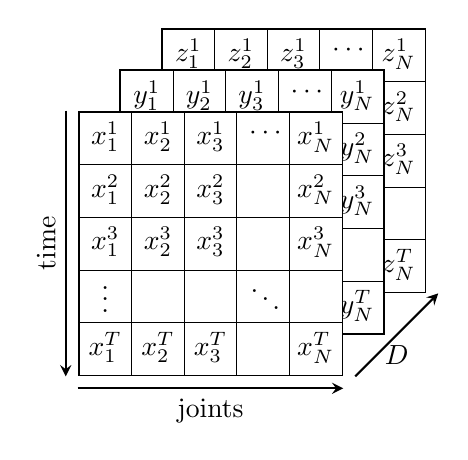
\begin{tikzpicture}[auto matrix/.style={matrix of nodes,
        draw,thick,inner sep=0pt,
        nodes in empty cells,column sep=-0.2pt,row sep=-0.2pt,
        cells={nodes={minimum width=1.9em,minimum height=1.9em,
         draw,very thin,anchor=center,fill=white,
         execute at begin node={%
         $\vphantom{x_|}\ifnum\the\pgfmatrixcurrentrow<4
           \ifnum\the\pgfmatrixcurrentcolumn<4
            {#1}^{\the\pgfmatrixcurrentrow}_{\the\pgfmatrixcurrentcolumn}
           \else 
            \ifnum\the\pgfmatrixcurrentcolumn=5
             {#1}^{\the\pgfmatrixcurrentrow}_{N}
            \fi
           \fi
          \else
           \ifnum\the\pgfmatrixcurrentrow=5
            \ifnum\the\pgfmatrixcurrentcolumn<4
             {#1}^{T}_{\the\pgfmatrixcurrentcolumn}
            \else
             \ifnum\the\pgfmatrixcurrentcolumn=5
              {#1}^{T}_{N}
             \fi 
            \fi
           \fi
          \fi  
          \ifnum\the\pgfmatrixcurrentrow\the\pgfmatrixcurrentcolumn=14
           \cdots
          \fi
          \ifnum\the\pgfmatrixcurrentrow\the\pgfmatrixcurrentcolumn=41
           \vdots
          \fi
          \ifnum\the\pgfmatrixcurrentrow\the\pgfmatrixcurrentcolumn=44
           \ddots
          \fi$
          }
        }}}]
       \matrix[auto matrix=z,xshift=3em,yshift=3em](matz){
        & & & & \\
        & & & & \\
        & & & & \\
        & & & & \\
        & & & & \\
       };
       \matrix[auto matrix=y,xshift=1.5em,yshift=1.5em](maty){
        & & & & \\
        & & & & \\
        & & & & \\
        & & & & \\
        & & & & \\
       };
       \matrix[auto matrix=x](matx){
        & & & & \\
        & & & & \\
        & & & & \\
        & & & & \\
        & & & & \\
       };
       \draw[thick,-stealth] ([xshift=1ex]matx.south east) -- ([xshift=1ex]matz.south east)
        node[midway,below] {$D$};
       \draw[thick,-stealth] ([yshift=-1ex]matx.south west) -- 
        ([yshift=-1ex]matx.south east) node[midway,below] {joints};
       \draw[thick,-stealth] ([xshift=-1ex]matx.north west)
         -- ([xshift=-1ex]matx.south west) node[midway,above,rotate=90] {time};
      \end{tikzpicture}
\end{center}
For our special case, or a matrix, it is the two-dimension case. Most of the operations acting on matrix can be indeed generalized, though it is most of the time more effective to define it on such. And, without being said, matrix's operations and functions, as well as its uses, are more rigorous perhaps, than the others $n$-dimension, and from array analogue itself. 

We will now jump to the more interpretable object that linear algebra will use. While array representation has its own meaning and usage, it is often poorly equipped to be used and utilized in a mathematical sense, simply because, as we said, it is a data structure only with no added purpose or interpretation of its structure. The next section, we will deal with two fundamental objects of linear algebra - the \textit{vector} and \textit{matrix} object.

\section{Vectors}

For a mathematical object, there are components to specify it details or particular structure. In the context of linear algebra, we deal with the variable spaces, where each mathematical object can take place. Usually, the structure that give rises to such space, which differs from case-to-case basis of different fields, is called a \textbf{mathematical structure}, in an informal sense. Linear algebra then, deals with the question of working on multi-descriptive objects, where its mathematical structure is considered of the \textbf{specification} that is needed to describe the mathematical object respectively. For example, by then, we can roughly get the mathematical object of real number, in the structure $\mathbb{R}$, to be a zeroth-order object by linear algebraical means. That is, it can be specified using a singular "point" - its own quantification value. Then, for complex number of the form $x= a+ bi$, then it can be then considered a first-order object in such sense, simply because its parameter can be, informally, listed as one row or one column, and each contains the previous zeroth-order component. Such zeroth-order object, if they are of a specific field, for example, the field of real number $\mathbb{R}$, then we have a special name for it: a \textbf{scalar}\index{scalar} on the field $\mathbb{R}$. Then, for a first-order complex number space $\mathbb{C}$, we can then call it to be the two-dimensional space on the field $\mathbb{R}$. By such, we have considered the singular complex space $\mathbb{C}$ to contains \textbf{vectors}\index{vector} of which takes zeroth-order component over $\mathbb{R}$ - two of them, that is. 

The more nominal example that one can think of, and will be implied throughout the chapter, is the description of a \textit{directed object}, or a \textit{directed path}. For example, the direction of the displacement in space of a plane, the acceleration accompanied by a car, the direction of rotation of a geometrical shape, or the direction in which the gradient is, for the landscape of a function. Such cannot be described, usually, by one singular value. It needs to be of something with magnitude; and some expression of direction. This is fulfilled by vector itself. 

If we think only vectors and scalar as mathematical object but on the side of data representation, it is rather easy to see the intuitive necessity of such. Many things require more than just one value, or numerical representation to defines its mathematical form. Such can be said of many physical notions, from forces - if your world is not one-dimensional, that is; or velocities, accelerations, positions, directions, et cetera. Any such entity will require more than one specification, and often, it can be reached with the simple composition of many single values together. This, form the notion of vector as we have above. Additionally, we also note that again, we would be dealing with analytical, numerical objects. So, vectors and the like will be plenty of operations and actions on it, as well as the nuance accompanied. 

It is then, rather more detail for once, to talk of the more reduced notion of a vector. The more physical, deliberate definition hence specifies the vector by its apparent properties - an object of both \textit{magnitude} and \textit{direction}. Do note that this definition can be extended for the other interpretations, as we see below: 
\begin{definition}[Vector]
    A (nonzero) \textbf{vector} $\vec{v}$, or $\mathbf{v}$, is a quantity or object with both \textit{magnitude} and \textit{direction}. It is also expressed by its \textit{vector components}, of which we denote as $\vec{v}=(v_1, v_2,\dots,v_n)$, for all $v_i$, $i=1,\dots,n$ as the $i$th component of $\vec{v}$. The requirements that a vector and operations on it must satisfy, and the space to specify such vector constitute a \textbf{vector space}. 

    Geometrically, a vector $\mathbf{v}$ is specified also by its segment drawn from a point $P$ (called \textbf{initial point}) to point $Q$ (called \textbf{terminal point}). Its magnitude is then the length of the segment, denoted by $\lvert\lvert \vv{PQ}\rvert \rvert$, and its \textbf{direction} is the same as of the directed line segment. The \textbf{zero vector} is the generalization of a point, denoted $\mathbf{0}$.
\end{definition}

We will leave the vector space and structure to later section on the mathematical structure of linear algebra itself. For now, we would consider the vector in its sense of a data structure, somewhat. Our notation of a vector is then pretty similar to the first-order array, or one-dimensional array in previous section. A vector $\mathbf{v}$ is hence presented as: 
\begin{equation}
    \mathbf{v} = \begin{pmatrix}
        v_{1} & v_{2} & v_{3} & \dots & v_{n}
    \end{pmatrix}
\end{equation}

or, in a vertical form, 

\begin{equation}
    \mathbf{v} = \begin{pmatrix}
        v_{1} \\
        v_{2} \\ 
        v_{3} \\
        \vdots \\
        v_{n} 
    \end{pmatrix}
\end{equation}

Notationally, they are called the \textbf{row vector} and the \textbf{column vector}. For now the differences are irrelevant - they specify the same object, and the same vector. The subtleties only comes when we consider certain interpretation and structure with the 'row' and the 'column' - which hints at matrix. 

Under such context, the \textit{dimension} is the length of the component description, or the number of component that a vector has. If a vector is in the special case where its value is zero (we work on maths, and it is numerical), then we say that it is t\textit{he $i$th-flatten vector over $n$-space}, where $n$ is its dimension. 

For vectors, there are certainly some special vectors. The \textbf{zero vector}, denoted $\mathbf{0}$ or $\vec{0}$, is the conception of singular free point, with respect to any particular reference coordinate frame. That is, a singular special point called the \textbf{origin} that has zero magnitude and zero direction. Similarly, there is the \textbf{unit vector}, denoted $\mathbf{1}$ or $\vec{1}$, or $\hat{i},\hat{j},\dots$ of lower-case characters, is defined such that $\lvert \mathbf{1}\rvert = 1$ for any given direction. A collection of unit vectors by specific conditions form the \textbf{coordinate system}. 

\begin{figure}[h!]
    \centering
    \includegraphics[width=0.6\textwidth]{img/vector1.png}
    \caption{An illustration of a vector in two-dimensional vector form in endpoints representation, and directional-magnitude representation.}
    \label{fig:vector1}
\end{figure}

There is a subtle detail in considering the notation for vector. One can see that the notation we used to represent vector is oddly similar to the notation used for $n$-dimensional points in an $n$-space, for example, the Euclidean space $\mathbb{R}^{3}$, which each point can be specified to be $(x,y,z)$ along each axis. Indeed, this is troublesome: if they are mixed up together, it would be difficult to distinguish the notation for coordinate system and one for the vector representation, especially in case of complex manipulation. We can offer certain solutions to this problem. The first one, is to re-interpret coordinate in a space just as similar as vectors - every point is actually a vector starting from the origin, travelling to the point itself. In such sense, a vector is considered like a path composition with respect to each axis, representing the total component path taken to specify the location of such point. Another way to think about a vector is that it is a \textit{compressed form}\index{compressed form} of two point specification - the \textit{starting point} $A_{s}$ and the \textit{endpoint} $B_{e}$, though often we would call them all together as endpoints. Then, a vector is the reduced representation for all pairs of endpoint such that, the vector is defined to be the final absolute path - or in terms of \textit{calculus of variations} sense, the shortest path - a straight line - toward the two endpoints. Any straight line, with direction that satisfies the component path from one endpoint to another is indeed, that one vector; or simply speaking. The direction is characterized by indeed, the order of the path, either from $A$ to $B$ or $B$ to $A$, and also based off their intrinsic location. In such representation, we separate the endpoints from the vectors - an endpoint has no direction and is dimensionless, stationary, while a vector specifies a path from two endpoints together, of the total difference between the two endpoints. In the end, though it is based in the interpretation of the case study, and what structures are considered. In a more advanced situation, one can also specify a point scalar as an element of a manifold, and a vector as an element of the tangent space to such manifold. 

Two vectors are equal if the components used to specify them are the same. Geometrically, it means they have the same magnitude and direction. \footnote{Settle aside the expression of component for a vector, usually, we can get a lot of the properties and actions on vector using only their intrinsic, geometrical interpretation, that is, the magnitude-direction expression for a vector (as illustrated in Figure~\ref{fig:vector1}). Previously, we have said that anything of certain magnitude and direction, or path, between two endpoints, is the same vector. As we are concerned of here, it is true that only the magnitude and direction of the vector are significant; hence consequently, we regard vectors with the same magnitude and direction as being equal irrespective of their position. This is true for the geometry of a vector, as we guarantee.}
\begin{definition}
    Two nonzero vectors are \textbf{equal} if they have the same magnitude and the same direction. Any direction with zero magnitude is equal to the zero vector. 
\end{definition}

Although we defined zero vector and equal magnitude, we still do not know for sure what can be used to make such definition operational. To tackle this, we have to define the notion of vector length, in the respective reference frame, and of respective measure, for example, in $\mathbb{R}$ or $\mathbb{Z}$. 

Recalling that the distance between two points $P(x_{1},x_{2},x_{3})$ and $Q=(y_{1},y_{2},y_{3})$ in the Euclidean space $\mathbb{E}^{3}=\mathbb{R}^{3}$\footnote{This equivalency is more on convention than not. Some books will say it being the same, some books will regard Euclidean space of higher-dimension than real space. However, a property holds in those definitions is that Euclidean space is defined without special origin. Furthermore, consider the pure vector space $\mathbb{R}^{3}$. If we grant it the inner product, it becomes Euclidean since one of the requirement for a space to be Euclidean, is for Euclid's axiom to hold. That is why sometimes we call Euclidean space the special case of real vector space.} is such that
\begin{equation}
    d(P,Q) = \sqrt{(y_{1}-x_{1})^{2} + (y_{2}-x_{2})^{2} + (y_{3}-x_{3})^{2}}
\end{equation}
Using such, we define the following as the vector \textbf{magnitude}:
\begin{theorem}[Vector magnitude]
    For a vector $\mathbf{v}=(a,b,c)$ in $\mathbb{R}^3$, the magnitude of $\mathbf{v}$ is: 
    \begin{equation}
        \lvert\lvert \mathbf{v} \rvert\rvert = \sqrt{a^{2}+b^{2}+c^{2}}
    \end{equation}
\end{theorem}
This can be scaled up or down for any given $n$.
\begin{proof}
    By definition of vector, its magnitude is the length of the segment. Arbitrary specification of end-points (endpoint-independent) property gives $(a,b,c)$ the component length with respect to each dimension. The rest follows. Also notice we can prove by exhaustion for all permutation of choice of $a,b,c$. 
\end{proof}

We have been introduced to the notion of vector. Naturally, a question should arise: what can we do with it, and with many of it? Fortunately, we have options for such aspect. For vectors, operations to be investigated would be two operations, the addition operation and the scalar multiplication for the time being. Let's begin with addition.

\begin{theorem}[Vector sum]
    The \textbf{sum} of vectors $\mathbf{v},\mathbf{w}$, denoted by $\mathbf{v}+\mathbf{w}$ is obtained by translating $\mathbf{w}$ so that its initial point is at the terminal point of $\mathbf{v}$, the initial point of $\mathbf{v}+\mathbf{w}$ is the initial point of $\mathbf{v}$, and the endpoint is the new terminal point of $\mathbf{w}$.
\end{theorem}

In component form, we can get, 
\begin{equation}
    \mathbf{v} + \mathbf{w} = \begin{pmatrix}
        x_{1}\\
        x_{2}\\
        \vdots\\
        x_{n}
    \end{pmatrix}
    + \begin{pmatrix}
        y_{1}\\
        y_{2}\\
        \vdots\\
        y_{n}
    \end{pmatrix}
    =
    \begin{pmatrix}
        x_{1}+y_{1}\\
        x_{2}+y_{2}\\
        \vdots\\
        x_{n}+y_{n}
    \end{pmatrix}
\end{equation}
This operation only happens if they have the same dimension. However, we can mitigate this partially by the following convention. 
\begin{lemma}
    If $\mathbf{v}$ and $\mathbf{w}$ acts on each other where $\dim{(\mathbf{v})}=n\neq m = \dim{(\mathbf{w})}$, then: If $n>m$, $\mathbf{w}$ is extended of zero value in the additional dimension; if $n<m$, $\mathbf{v}$ is applied of the same.\footnote{We have not defined the vector space yet at this point. However, based on the notion of dimension described before, and considering the space of which we put on the dimension notion in to specify the vectors, this result is palpable. Nevertheless, if we can define a vector space, then it means either one contains the \textbf{vector subspace} of the other.}
\end{lemma}
The behaviour of this sum is intuitive - linking directed line altogether with each other. Because of this, we will have the following observation. 
\begin{theorem}[Parallelogram law]
    The sum of two vectors $x$ and $y$ that acts at the same point $P$ is the vector beginning at $P$ that is represented by the diagonal of parallelogram having $x$ and $y$ as adjacent sides. 
\end{theorem}
\begin{question}
    Can you realize the parallelogram law in analytical terms of its coordinate?
\end{question}
This can be illustrated in Figure~\ref{fig:vector_sum_parallel}. Do note that it is more or less, a not so trivial point. 
\begin{figure}[h!]
    \centering
    \includegraphics[width=0.8\textwidth]{img/vector_sum-001.png}
    \caption{The \textbf{parallelogram law} for vector addition of two vectors $x$ and $y$ on adjacent side.}
    \label{fig:vector_sum_parallel}
\end{figure}
Aside from additive operation, vector can also be multiplied, albeit restricted to multiplying with a scalar $\lambda$ only \footnote{Since this is not a textbook, you should have noticed by now, if you have educations of linear algebra beforehand, that there exists the \textbf{vector product} of the special case of matrix multiplication. However, of such is usually not the standard interpretation of vector, and is rather specified with meanings than abstracted notion --- that is to say that the scope of the `vector' considered in this section is not that wide, yet.}. For this, of a vector $\mathbf{v}$, we define $\lambda\cdot \vec{v}$ as: 
\begin{equation}
    \lambda\mathbf{v} = 
    \lambda\begin{pmatrix}
        x_{1}\\
        x_{2}\\
        \vdots\\
        x_{n}\\
    \end{pmatrix}
    =
    \begin{pmatrix}
        \lambda x_{1}\\
        \lambda x_{2}\\
        \vdots\\
        \lambda x_{n}\\
    \end{pmatrix}, \quad \lambda \in \mathbb{R}
\end{equation}
The scalar is multiplied, component-wise, for each element of the vector. Non-algebraically, this is effectively the action of scaling with respect to direction of a given vector by $\lambda$ amount(s). By now, you might also have noticed that we switch between analytical (algebraical, if you like) and geometrical description, and this is not unnatural, and sometimes offer understanding that complements the other method. 
\begin{definition}[Scalar, multiplication]
    We define a \textbf{scalar} as a quantity equal to a single component, and geometrically a point\footnote{Interesting fact. There are two entries on which the word scalar was used. The word scalar derives from the Latin word scalaris, an adjectival form of scala (Latin for "ladder"). The first use is in François Viète's Analytic Art (In artem analyticem isagoge) (1591), where it is written that "Magnitudes that ascend or descend proportionally in keeping with their nature from one kind to another may be called scalar terms.". Another one is by William Rowan in the 19th century, to convey the sense of something that could be represented by a point on a scale or graduated ruler.}. For a scalar $k$ and a nonzero vector $\mathbf{v}$, the \textbf{scalar multiple} of $\mathbf{v}$ by $k$, denoted by $k\mathbf{v}$, is the vector whose magnitude is $\lvert k\rvert \lvert \lvert \mathbf{v}\rvert\rvert $, same direction as $\mathbf{v}$ for $k>0$ and reverse if $k<0$, and is the zero vector if $k=0$. For the zero vector $\mathbf{0}$, we define $k\mathbf{0}=\mathbf{0}$ for any scalar $k$. 
\end{definition}

Using our analytical formalism, we can try to prove those operations. Indeed, let's see how that might potentially work. 
\begin{theorem}
    Let $\mathbf{v}=(v_{1},v_{2},v_{3})$, $\mathbf{w}=(w_{1},w_{2},w_{3})$ be vectors in $\mathbb{R}^{3}$, let $k$ be a scalar. Then: 
    \begin{enumerate}[itemsep=1pt,topsep=0pt]
        \item $k\mathbf{v}=(kv_{1},k v_{2})$. 
        \item $\mathbf{v}+\mathbf{w}=(v_{1}+w_{1},v_{1}+w_{3})$. 
    \end{enumerate}
\end{theorem}
\begin{proof}
    (a) We would be using basic geometry for such purpose of assumptions for further proofs. Without loss of generality, we assume that $v_{1},v_{2}>0$ (the other possibilities are handled in a similar manner). If $k\neq 0$, then $(kv_{1},kv_{2})$ lies on a line with slope $kv_{2}/kv_{1}=v_{2}/v_{1}$, which is the same as the slope of the line on which $\mathbf{v}$ (and hence $k\mathbf{v}$ lies), and $(kv_{1},kv_{2})$ points in the same direction on the line as $k\mathbf{v}$. Furthermore, 
    \begin{equation}
        \lvert (kv_{1},kv_{2}) \rvert = \sqrt{(kv_{1})^{2}+(kv_{2}^{2})} = \sqrt{k^{2}v_{1}^{2} + k^{2}v_{2}^{2}} = \sqrt{k^{2}(v^{2}_{1}+ v_{2}^{2})} = \rvert k \lvert \sqrt{v_{1}^{2}+v_{2}^{2}} = \lvert k \rvert \lvert \lvert \mathbf{v}\rvert \rvert 
    \end{equation}
    This indicates that they have the same magnitude and direction. This concludes the proof. 

    (b) Without loss of generality, we assume that $v_{1},v_{2},w_{1},w_{2}>0$. We see that when translating $\mathbf{w}$ to start at the end of $\mathbf{v}$, the new terminal point of $\mathbf{w}$ is $(v_{1}+w_{1},v_{2}+w_{2})$, so by definition of $\mathbf{v}+\mathbf{w}$ this must be the terminal point of it. This concludes the proof.  
\end{proof}

\subsection{Properties of vectors}
With a lot of objects in mathematics, they can always be described in mainly two ways: either analytically (algebraically) or geometrically. Let's investigate the geometrical view first. 
\subsubsection{Interpretation of references}
A vector can be considered to be a \textit{free object} in the geometrical space. That is, it is not bounded by coordinates likes points, or geometrical structure embedded within the space by specification. Rather, it is free in the sense that the vector is similar to itself, by means of linear translation throughout the geometrical space, for example, moving the vector left or right, up or down. Analytically, it means that a vector description refers to its designed specification, and not positional descriptions. What does this mean? I would want to say it in terms of some rigours, but certainly, it depends on the interpretation, at the foremost aspect, but that would be pretty much useless. For my own understanding, one can regard the description of a coordinate $(x,y,z)$ and a vector $x(x_1, x_2, x_3)$ by some subtleties, independent or dependent on the coordinate basis or not. A coordinate is dependent of the coordinate system, or the space specification, or the descriptors, because its component depends on each of the component space. Or, rather, it depends on the origin where everything is referenced from. Vector, on the other hand, use the notation a bit differently. Sure, it is still the path, or rather, if we are to treat it similarly to the indexing of an array, then it is similar to the array index to recognize an object's position. However, the descriptor is not taking positions or index, it is taking the relatively speaking, \textit{path, length} instead. Or rather, it is the compression of two values, just as we spoke up there. So each vector is actually representing: 
\begin{equation}
    \mathbf{x} = (x_{1},x_{2},x_{3},\dots,x_{n}) = (x_{1e}- x_{1b}, x_{2e}- x_{2b},\dots, x_{ne}- x_{nb}) 
\end{equation}
where the subscript $ie, ib$ is the $i$th component's end point and begin point. Now, I have to admit I don't know how to get this to be further than it is. Then, we would have the coordinate system using the pretty much special case of this system, \footnote{So, yeah, same notation, different interpretation. Especially when you consider that you can, and indeed would likely want to write them down together. Though, because of this, most of the time, we would consider them to be relatively the same, because as we said, we can translate them down to anywhere, as long as the descriptor, which specifies the direction, magnitude, et cetera, stays the same - which includes the origin point. }
\begin{equation}
    x = (x_{1},x_{2},x_{3},\dots,x_{n}) = (x_{1e}- 0, x_{2e}- 0,\dots, x_{ne}- 0) 
\end{equation}
\subsubsection{Basic vector algebra}
Moving on, for basic vector operations, we have the following. 
\begin{theorem}[Vector algebra]
    For any vectors $\mathbf{u},\mathbf{v},\mathbf{w}$, and scalar $k,l$, we have: 
    \begin{enumerate}[topsep=0.5pt,itemsep=1pt,label=(\emph{\alph*})]
        \item $\mathbf{v}+\mathbf{w}=\mathbf{w}+\mathbf{v}$ (Commutative Law)
        \item $\mathbf{u}+(\mathbf{v}+\mathbf{u})=(\mathbf{u}+\mathbf{v})+\mathbf{w}$ (Associative Law)
        \item $\mathbf{v}+\mathbf{0}=\mathbf{v}=\mathbf{0}+\mathbf{v}$ (Additive identity)
        \item $\mathbf{v}+(-\mathbf{v})=\mathbf{0}$ (Additive Inverse)
        \item $k(l\mathbf{v})=(kl)\mathbf{v}$ (Associative law for scalar multiplication)
        \item $k(\mathbf{v}+\mathbf{w})=k\mathbf{v}+k\mathbf{w}$ (Distributive law)
        \item $(k+l)\mathbf{v}=k\mathbf{v}+l\mathbf{v}$ (Distributive law)
    \end{enumerate}
\end{theorem}
\begin{proof}
    Proved using algebraic manipulation or geometrical proofs. 
\end{proof}
Notice that using the commutative law, we gain the parallelogram law proof, since it permits the motion of attaching different vector to the end of each other. For $n$ vectors apparent, any 2-permutation resolves the same theorem. 
\subsubsection{The `missing' operations}
As far as elementary operations are concerned, we notice some operations that `seem to be missing'. That are the \textit{vector-vector multiplication} and \textit{scalar-vector addition}. We can multiply and add scalar to scalar, multiply scalar to vector, add vector to vector, but not the other two. 

\section{Matrix}

Matrix is the special type of array that is used in construction of linear algebra. Specifically, it is array, in special consideration, and added structures. Mathematically, it is defined as followed. 
\begin{definition}[Matrix]
    A matrix $A$ is a two-dimensional array, with dimensions' size of $m\times n$ for $m$ is the horizontal dimension (the column) and $n$ the vertical dimension (the column). \footnote{This is just a normal convention.}. For each element $a\in A$ of matrix $A$, it is indexed by $a_{ij}$ for $1\leq i \leq m$ and $1\leq j \leq n$. It is represented as: 
    \begin{equation}
        A = \begin{pmatrix}
            a_{11} & a_{12} & a_{13} & \dots & a_{1n}\\
            a_{21} & a_{22} & a_{23} & \dots & a_{2n}\\
            \vdots & \vdots & \vdots & \ddots & \vdots \\
            a_{m1} & a_{m2} & a_{m3} & \dots & a_{mn}\\
        \end{pmatrix}
    \end{equation}
\end{definition}

The bracket is pretty much cosmetic, though, to distinguish from the use of array and matrix, we will use $[\cdot]$ for array and $(\cdot)$ for matrices. 

Given such, what can we do with matrices? First, we can \textit{add} them together; given $A,B$ being two matrices, then $A+B$, the \textit{matrix addition} is defined as: 
\begin{equation}
A + B = \begin{pmatrix}
            a_{11} + b_{11} & a_{12} + b_{12} & a_{13} + b_{13}& \dots & a_{1n}+ b_{1n}\\
            a_{21} + b_{21} & a_{22} + b_{22} & a_{23} + b_{23}& \dots & a_{2n}+ b_{2n}\\
            \vdots & \vdots & \vdots & \ddots & \vdots \\
            a_{m1} + b_{m1} & a_{m2} + b_{m2} & a_{m3} + b_{m3}& \dots & a_{mn}+ b_{mn}\\
        \end{pmatrix}
\end{equation}
Furthermore, \textit{scalar multiplication} to a matrix is also available, and $\lambda A$ is defined as: 
\begin{equation}
    \lambda A = \begin{pmatrix}
            \lambda a_{11} & \lambda a_{12} & \lambda a_{13} & \dots & \lambda a_{1n}\\
            \lambda a_{21} & \lambda a_{22} & \lambda a_{23} & \dots & \lambda a_{2n}\\
            \vdots & \vdots & \vdots & \ddots & \vdots \\
            \lambda a_{m1} & \lambda a_{m2} & \lambda a_{m3} & \dots & \lambda a_{mn}\\
        \end{pmatrix}
\end{equation}
For multiplication, the simplest operation that can be realized from component-based multiplication is the \textbf{Hadamard multiplication} or component based multiplication, denoted as $A\odot B$, defined as: 
\begin{equation}
    A\odot B = \begin{pmatrix}
            a_{11} \odot b_{11} & a_{12} \odot b_{12} & a_{13} \odot b_{13}& \dots & a_{1n}\odot b_{1n}\\
            a_{21} \odot b_{21} & a_{22} \odot b_{22} & a_{23} \odot b_{23}& \dots & a_{2n}\odot b_{2n}\\
            \vdots & \vdots & \vdots & \ddots & \vdots \\
            a_{m1} \odot b_{m1} & a_{m2} \odot b_{m2} & a_{m3} \odot b_{m3}& \dots & a_{mn}\odot b_{mn}\\
        \end{pmatrix}
\end{equation} 
\begin{remark}
    Let $\mathbf{A}=diag(a_{1},\dots,a_{n})$ in $\mathbb{R}^{m\times n}$, and $\mathbf{B}\in\mathbb{R}^{n\times k}$. Define also a vector $\mathbf{a}=(a_{1},\dots,a_{n})^{\top}\in\mathbb{R}^{n}$, which represents the diagonal of $\mathbf{A}$. Then $$\mathbf{AB}=[\mathbf{a}\dots \mathbf{a}]\circ \mathbf{B}$$
The former takes $\mathcal{O}(n^{2}k)$ operations, while the latter takes only $\mathcal{O}(nk)$ operations, which is one magnitude faster. 
\end{remark}
All of our operations up to this point has been with two matrices $A,B$ of the same shape, that is, $m\times n$ for both. What happens if they are now then different? Either we can justify the operation by `extending it', however, usually, this requires discrete specific description for that to be able to be considered. Hence, matrix-matrix operations like such above is restricted of the entry shape. 

Finally, we have one more important operation to be defined here at last. For two matrices $A,B$ of shape $m\times n$ and $n\times p$, the \textbf{matrix multiplication} operation that outputs an $m\times p$ matrix, is available as: 
\begin{equation}
    A\times B = \begin{pmatrix}
        a_{11} & \dots & a_{1n} \\
        a_{21} & \dots & a_{2n} \\
        \vdots & \ddots & \vdots \\
        a_{m1} & \dots & a_{mn}
    \end{pmatrix}
    \begin{pmatrix}
        b_{11} & \dots & b_{1p} \\
        b_{21} & \dots & b_{2p} \\
        \vdots & \ddots & \vdots \\
        b_{n1} & \dots & b_{np}
    \end{pmatrix} = 
    \begin{pmatrix}
        c_{11} & \dots & c_{1p} \\
        c_{21} & \dots & c_{2p} \\
        \vdots & \ddots & \vdots \\
        c_{m1} & \dots & c_{mp}
    \end{pmatrix}
\end{equation}
where \begin{equation}
    c_{ik} = \sum_{j<n} a_{ij}b_{jk}
\end{equation}
For certain reason in the theory, or \textbf{matrix theory} and linear algebra in general, the matrix multiplication is explicitly defined only for such shape configuration. Otherwise, the matrix multiplication simply does not exist.
\begin{figure}[htb]
    \centering
    \includegraphics[width=0.4\textwidth]{img/jjgh.jpg}
    \caption{Illustration of matrix multiplication. Taken from \cite{ANDRILLI20101}.}
    \label{fig:matmuls}
\end{figure}
\begin{figure}[htb]
    \centering
    \includegraphics[width=0.4\textwidth]{img/matmulss.png}
    \caption{Illustration of matrix multiplication for $2\times 2$ shape.}
    \label{fig:matmuls2}
\end{figure}
\subsection{Special matrices, operations, and properties}
Matrix has quite a few of special types that is defined for either decomposing the many matrices, or to complement them in expression. Operations aside from basic `interactive operations' as above is also available, most of the time acting on the matrix by itself. Those operations, special matrices and properties are there to then draw out reasonable consequences and results. 
\subsubsection{Matrix shape}
Informally, A \textbf{matrix} is a rectangular array of numbers arranged in rows and columns. We say that a matrix $\mathbf{A}\in \mathbb{R}^{m\times n}$ is (given the entry field $\mathbb{R}$)
\begin{enumerate}[topsep=1pt,itemsep=1pt]
    \item A square matrix if $m=n$. 
    \item A long matrix if $m<n$
    \item A tall matrix if $m>n$
\end{enumerate}
A \textbf{diagonal} matrix is a square matrix $\mathbf{A}\in \mathbb{R}^{n\times n}$ whose off diagonal entries are all zero, so $a_{ij}=0$ for all $i\neq j$: 
\begin{equation}
    \mathbf{A}=\begin{pmatrix}
a_{11}  &  &  &  \\
 & \ddots  &  &  \\
 &  &  & a_{nn}
\end{pmatrix}
\end{equation}
A diagonal matrix is uniquely defined through a vector that contains all the diagonal entries, and denoted as follows:
\begin{equation}
    \mathbf{A}=\mathrm{diag}(1,2,\dots,n)=\mathrm{diag}(\mathbf{a})
\end{equation}
Using the diagonal matrix, we gain the following result. 
\begin{proposition}[Diagonal multiplication]
    Given two matrices $A,B$ of compatible shape. Then, if one is a diagonal matrix, denoted $A_{diag},B_{diag}$, then the following is true. 
    \begin{equation}
        A_{diag}\mathbf{B}=\begin{pmatrix}
a_{1}  &  &  &  \\
 & \ddots  &  &  \\
 &  &  & a_{n}
\end{pmatrix}\begin{pmatrix}
\mathbf{B}(1,:) \\
\vdots \\
\mathbf{B}(n,:)
\end{pmatrix}=\begin{pmatrix}
a_{1}\mathbf{B}(1,:) \\
\vdots \\
a_{2}\mathbf{B}(2,:)
\end{pmatrix}
    \end{equation}
and 
\begin{equation}
    \mathbf{A}B_{diag}=\begin{pmatrix}
\mathbf{A}(1,:) \\
\vdots \\
\mathbf{A}(n,:)
\end{pmatrix}\begin{pmatrix}
b_{1}  &  &  &  \\
 & \ddots  &  &  \\
 &  &  & b_{n}
\end{pmatrix}=\begin{bmatrix}
b_{1}\mathbf{A}(:,1)\dots b_{N}\mathbf{A}(:,n)
\end{bmatrix}
\end{equation}
\end{proposition}

The two unit matrices that is often seen is the \textbf{identity} and \textbf{zero} matrix. Given the name, $\mathbf{I}$ is used to denote the identity matrix: $$\mathbf{I}=\begin{bmatrix}
1 & 1 & \dots & 1 \\
1 & 1 & \dots & 1 \\
\vdots  & \vdots  & \ddots  & \vdots \\
1 & 1  & \dots & 1
\end{bmatrix}$$
and $\mathbf{O}$ for the zero matrix, 
$$\mathbf{O}=\begin{bmatrix}
0 & 0 & \dots & 0 \\
0 & 0 & \dots & 0 \\
\vdots  & \vdots  & \ddots  & \vdots \\
0 & 0  & \dots & 0
\end{bmatrix}$$
with their sizes implied by the context, entries of all $1$ or $0$, respectively. 

\subsubsection{Transpose, inverse, trace and rank}
Given a matrix $A$, then $A^{\top}$ is called the \textbf{transpose} of $A$ for its shape reversed, $A_{m\times n}$ to $A'_{n\times m}$ with $b_{ij}=a_{ij}$ for all $i,j$. A square matrix $\mathbf{A}_{n\times n}$ is said to be symmetric if $\mathbf{A}^{\top}=\mathbf{A}$. We have the following result. 
\begin{proposition}
    Let $\mathbf{A}$ be a matrix of size $m\times n$, $\mathbf{B}$ be a matrix of size $n\times p$. Then, 
    \begin{enumerate}[itemsep=1pt,topsep=1pt]
        \item $(\mathbf{A}^{\top})^{\top}=\mathbf{A}$.
        \item $(k\mathbf{A})^{\top}=k\mathbf{A}^{\top}$
        \item $(\mathbf{A}+\mathbf{B})^{\top}=\mathbf{A}^{\top}+\mathbf{B}^{\top}$
        \item $(\mathbf{AB})^{\top}=\mathbf{B}^{\top}\mathbf{A}^{\top}$
    \end{enumerate}
\end{proposition}
If we consider next the notion of the \textbf{inverse} of a matrix, the true, classical inverse definition works only for square matrix, by definition. 
\begin{definition}[Matrix inverse]
    A \textit{square matrix} $\mathbf{A}\in\mathbb{R}^{n\times n}$ is said to be invertible if there exists another square matrix of the same size $\mathbf{B}$ such that $\mathbf{AB}=\mathbf{BA}=\mathbf{I}$. 
\end{definition}
In this case, $\mathbf{B}$ is called the matrix inverse of $\mathbf{A}$ and denoted as $\mathbf{B}=\mathbf{A}^{-1}$. We have the following property: 
\begin{proposition}
    Let $\mathbf{A},\mathbf{B}$ be two invertible matrices of the same size, and $k\neq 0$. Then 
    \begin{align}
        (k\mathbf{A})^{-1} & = \frac{1}{2}\mathbf{A}^{-1}\\
        (\mathbf{AB})^{-1} & = \mathbf{B}^{-1}\mathbf{A}^{-1}\\
        (\mathbf{A}^{\top})^{-1} & = (\mathbf{A}^{-1})^{\top}
    \end{align}
\end{proposition}
The \textbf{trace} of a square matrix $A\in \mathbb{R}^{n\times n}$ is defined as the sum of the entries in its diagonal, such that: 
\begin{equation}
    \mathrm{trace}(A)=\sum_{i}a_{ii}
\end{equation}
We sometimes denote it as $\mathrm{Tr}(A)$. Clearly, $\mathrm{Tr}(A)=\mathrm{Tr}(A^{T})$. Trace is a \textbf{linear} operator, so $\mathrm{Tr}(kA)=k\mathrm{Tr}(A)$ and $$\mathrm{Tr}(A+B)=\mathrm{Tr}(A)+\mathrm{Tr}(B)$$ If $A$ is an $m\times n$ matrix and $B$ is an $n\times m$ matrix then $$\mathrm{Tr}(AB)=\mathrm{Tr}(BA)$$ Note that as matrices, $AB$ is not necessarily equal to $BA$. 

Continuing, for a matrix $A$, the largest number of linearly independent rows (or columns) contained in the matrix is called the rank of $A$, denoted $rank(A)$. 

A square matrix $P\in\mathbb{R}^{n\times n}$ is said to be of full rank, or \textit{nonsingular}, if $rank(P)=n$, otherwise, it is said to be rank deficient (or \textit{singular}). A rectangular matrix $A\in\mathbb{R}^{m\times n}$ is said to have full column rank if $rank(B)=n$. Similarly, a rectangular matrix $A\in\mathbb{R}^{m\times n}$ is said to have full row rank if $rank(B)=m$. 


\include{content/math/mathc3}
\include{content/math/mathc4}
\include{content/math/mathc5}
%------------------------------------------- PART A. CLASSICAL -------------------------------------------%
\clearpage 
\partepigraph{The classic of the old, the foundation of the past. What is of their uses? Theory and theory. All those conjecture and ideas, in one single place.}{P. Q. Doyle}
\part{Theory}
\chapter{Classical mathematical modelling}
Often time when we refer to modelling, we consider it to be \textit{mathematical modelling} instead. Because our interest aligns with such, we will talk all about modelling, and its principle, in this section. 

We begin this section to mathematical modelling and simulation with an explanation of basic concepts and ideas. Generally, this includes exactly defining the terms \textbf{system, model, simulation, mathematical model}, and related notions or subcontext.  

We also discuss and analyse on the reflections of the objective of mathematical modelling, and simulation, on characteristics of "good" models, and classification of mathematical models. Though it is strongly advised to take the following section in a \textit{classical sense}, as we would eventually find out, that the notions and concepts presented here will be vastly outdated - and hence needs quite a bit of update to stay up with the current state-of-the-art theory. 

Our starting point is the complexity of the problems treated in science and engineering, because from here, is the first case we even need to create a \textbf{model}. There exists a lot of \textbf{non-mathematical models} in the past, however, and we shall see how the language of mathematics will help in this role. \cite{VeltenetalMathematicalModelling} will be the main text of this section. 

\section{The supposed goal of modelling}

In science, a \textit{system} refers to the object of interests, which can be a part of nature (atoms, etc), or an artificial technological system. Principally, we do this all days, with similar approach to isolate the problem into its respective system. 

The more \textbf{complex} a system is, the harder it is for dealing with the objects in that system, and the more intricate relationships and factors contributes to specific observations and problem that dilute the solution. It is the genuine task of \textbf{scientist} and \textbf{engineers} then, to deal with complex systems, and be effective at it, to deal with the extended complexity requires to solve the problems inferred in the system itself. 

For a very complex system, the first step would be simple - be simple. That is, we use \textbf{simplification} of such system to start solving it. Usually, to solve specific problems given a system, a simplified view can pinpoint exactly the ergonomic of the problem - what is important, what to discard, and what to consider. 

Take an example of a car. Suddenly, it does not start. 90\% of the time, trying to look into its tank, or battery, will solve the problem. While doing this consciously, what we have done is the simplification of the concept of a car. A car, by itself, is a very complex system full of mechanical moving parts and intricate connections. However, under the question of \textit{why it cannot run}, a simplified picture focuses on \textit{what enables it to run} in the first place, result in pinpointing the first two choices - which equates to the fact that 'a car need fuels to run, similarly needs energy to work'. 

This simplified picture is appropriate, \textit{most of the time}. If this does not work, our focus shifts to the next simplification - the wheel differential is not working. And that continue. The ergonomic here works similar to deduction and elimination. Once factors are eliminated, the one remaining will be the root of the problem. Instead of solving the system immediately as a whole, we targeted it by analysing the components it brings. 

In another different way, simplification does help with understanding complex system, is the effect of \textbf{scale}. If one want to study photosynthesis, they would go for a single cell instead of millions. By certain assumptions and pervious conjectures, we then can analyse the single cell, and generalize it for the entire millions by uniformity. If one wishes to learn how the brain works, they would focus on the smallest component that makes up the brain first. 

To break up the complexity of a system under consideration, we need to use simplified descriptions of that system - or \textbf{models}. This can be done either by elimination, abstractions, or else. But first, we need the definition of a model. 

\section{Models, systems, and questions}
For the beginning of the discussion, we would like to examine the concept of a model, from a given perspective. The following definition follows from Marvin Minsky (1965): \index{model} 

\begin{definition}[Model]
    To an observer $B$, an object $A^{*}$ is a \textbf{model} of an object $A$ to the extent that $B$ can use $A^{*}$ to answer question that interest him about $A$. 
\end{definition}

The definition is pretty much very "purposeful" definition, one can clearly see the dependency of the existence of a model $A^{*}$ onto an object $A$. Note, that in the definition it implies that \textit{no model is perfect} - by the priori, there exists the observer $B$, hence their interpretation might, or perhaps will be subjective. For example, the model of probability that it will be raining in Detroit being 80\% in the first two days, and 20\% for the remaining 5 days of the week, can be interpreted differently as 100\% percent raining for the first two, and 0\% otherwise, assume the record is correct. But under the consideration and the problem setting, the model is indeed perfect by itself. The definition is hence a \textit{formal definition}, in the sense that it operates with terms such as \textit{objects} or \textit{observer} that are not defined in a strict, axiomatic sense in mathematics. In fact, it is not so effective to think of defining axiomatically, since we can have both informal and formal axiomatization.\footnote{The issue here might be more nitpicking than not. But, under specified circumstances, we can say that \textit{formalism} works by describing and structure the system in a strict sense, without relying on meaning, and pure specification. While *axiomatization* focus on the structuring itself - will it is the way that everything is built upon the set of \textit{axioms}, no further question, held as truth, in which all other results follow? Hence, in such sense, formalism looks into the description and the abstraction of objects living in such space, while axiom determine the logic and dependency that follows. }

An important aspect of the above definition is the fact that it includes the purpose of the model, which helps us to solve the question and bring solution to problems. This is the reason for the principle often used as the best model, and in machine learning, associated with Lord of Occam's principle - the best explanation is the \textit{simplest} one on the tray. But this point comes with doubts. 

It turns out, that simplicity is not always the good one. On the contrary, it is the bad one, depends on the situation arises, and so is the complex one. There are inquiries taken in care of the word \textit{simple} and \textit{complex} in such scenario. Often time, sometime is called \textbf{simple} if its descriptions are minimal, along with assumptions that go aside with it. These assumptions is a lot of time the failure of the simple system. A system is called \textbf{complex}, if it contains rigorous descriptions, with what was assumed to be constrained, often in a precise and affective manner. Specification of such aspect, which brings more consideration in, is what makes a system complex. As per our example of the car, the simplified notion only comes, when we assume all others components are negligible, and focus on the assumption that what matters is the battery and the fuel cell. 

The issue here then lies, with the notion of the \textit{question} and \textit{problems} instead with the simple and complex dilemma. Sometimes, simple question requires complex models. Sometimes, complex problems require simple models. Sometimes, complex problems require gradually increased complexity of a model. The principle on the focus of the teleological nature of the problem the model pertains to, only applies in the \textit{ergonomic sense} of \textit{reasonable explanation} - often time, this reasonable explanation can be 30\% correct, but still, they are correct 30 out of 100. Teleological means purpose - or at least is interpreted as - and if we only constrain ourselves to the purpose, \textit{only the purpose}. Taken the example of linear regression to a particular problem that is not linear. Sure, we have satisfied the purpose, but the accuracy will inherently very low because it is trying to do what it cannot do - trying to figure out the nonlinear relationship, while constrained to be linear. 

Under such term, we might as well think this principle of \textit{best model} as pretty misleading. Rather, we say, we have the principle of \textit{effective model}. An effective model is a model that serves its purpose, specified correctly, given that the \textit{relative complexity} falls into the range of what can be considered \textit{relatively simplification} of the space of all possible solutions. That is, it can be simple, but not the simplest.  This, still, does not guarantee that the effective model will be better than the more complex model. In fact, it only establishes the lower bound. We ought to remember that. \textbf{Oversimplification} is a bad thing, while \textbf{overcomplication} also retains in the spectrum.

Returning to the issues we raised it is also true that the non-exact notion of simplicity and complexity is rather, \textbf{complex}. To do this though, we need to know what the 'purpose', or the question is required. A question is based on the system that it is in. In a complex system, a simple question is a hard one, and a complex question is a simple one, which is why it needs complex model to constrain it first to specifiable case. Hence, each question carries with it the *scope and freedom* of the question. In a simple space, a complex question is the harder one - unnecessary even - while the simple question fits with what the system is intended for. If the question is iterative, or expanding, this notion also follows. Overall, it is perhaps subjective to the frame of reference. 

\subsection{The modelling scheme}
Conceptually, the investigation of complex systems using models can be divided into the following steps: 

\begin{proposition}[Modelling and simulation scheme]
    The modelling and simulation scheme can be attained as followed: 
    \begin{enumerate}[noitemsep]
        \item \textbf{Definitions}: Definition of a problem that is to be solved, or of a question that is to be answered; and of a system, that is, a part of reality that pertains to this problem or question.
        \item \textbf{System analysis}: Identification of parts of the system that are relevant for the problem or question. 
        \item \textbf{Modelling}: Development of a model of the system based on the results of the system analysis step. 
        \item \textbf{Simulation}: Application of the model to the problem or question and derivation of a strategy to solve the problem or answer the question. 
        \item \textbf{Validation}: Does the strategy derived in the simulation step solve the problem or answer the question for real system?
    \end{enumerate}
\end{proposition}
In real modelling and simulation project, the \textit{system analysis} step can be very time-consuming. It will usually involve a thorough evaluation of the literature. In such step, experimental program is also a typical part. 

The modelling and simulation scheme focuses on the essential steps of modelling and simulation, giving a rather simplified picture of what happens in a concrete project. Though, as we spoke in the last section, start with the simplest possible model, and then generate a sequence of increasingly complex formulation, until the criteria is sufficed. 

\subsection{Simulation}
So far, we have given a definition of the term \textit{model} only. The above modelling and simulation schemes involve other terms, such as system and simulation, which might be viewed as implicitly defined. However, we shall make this to be more precise in meaning. In general, it can be as the following. \index{simulation}

\begin{definition}[Simulation]
    \textit{Simulation} is the application of a model with the objective to derive strategies that help solving a problem or answering a question pertaining to a system. 
\end{definition}
This definition, explicitly, also is defined to emphasize the purpose. Though, this purpose again, can be replication itself. So, the argument against replication as "l'art pour l'art" really does not help here that much. 

On the side note, as always, there is also the question of what kind of simulation we are talking about. If we follow the narrative of simplification, there can exist the physical simulation of a simplified system - by itself is also just a simulation in which physical realization of objects are needed. On the other hand, there is also the non-physical, in a sense, simulation, which makes use of particular information-encoded representation - or rather, a \textit{warped representation} using another physical system to interpret and simplify the physical realization that is done or used by the 'real thing', and go on with said representation or language. That is where we use computers or any representative system with computational power. This distinction might be detrimental in the process of solving the problem itself. 
\subsection{System}
Our view of systems is similar to a definition by certain someone who like being stuck in a roundabout: "A system is whatever is distinguished as a system". And then, the teleological principle-based definition is as follows: \index{system}

\begin{definition}[System]
    A \textit{system} is a collection or a collection of objects whose properties we want to study. 
\end{definition}

It is wise to notice in such, that a system can be deceiving. Taking an example, or rather, a typical scene often seen in the field of thermodynamic, there is the saying that "whoever breaks the second law, ultimately wields the power of infinite." - or rather, defying the second law of thermodynamic to gain infinite power, without putting in any work $W$. 

This prompted people to set up their own system, and try to make amend of the law. Many attempts tried to break the status quo (which might never be broken), and yet none works, more so being called crackpot, that guarantee the saying "the only issue of perpetual motion machines (the one that defies the second law) is to find where they hid the battery.". It's not always the battery every time, but the one that claims that the second law has been broken, always \textit{messes up their system}. By one way or another, their system is inconclusive - there are external influences, influx, or resources pouring in, that does not exist in the considered system. Hence, by extension, the 'infinite energy' comes from outer sources - undoubtedly infinite energy within the flaw system. 

So, long story short, perhaps, in the classical sense of the use of defining a system, please define it carefully. Or then someone will claim that you can create something out of nothing, that would be troublesome. 

\subsection{Conceptual and physical model}
As we have been saying on section about simulation, the same notion of realization in physical sense also manifests in the sense of conceptual or physical model. We will see about it. 

There are two types of model. There exists the \textit{conceptual (theoretical) model} \index{theoretical model}, which lives in a theoretical world without physical realization. This is where we have what is considered as \textit{thought experiment}, where certainly, with physical realization removed, the representative power of shooting reality up in the sky for unsurmountable scenario to be possible within theories - is allowed. 

Against it, such an experimental setting, that simplifies the problem of the engine to its smaller replica, and solve the problem directly on such replica is call the \textit{physical models} \index{physical model}. In contrast, as transparently presented, it is not only an idea in our mind, but also a real part of a physical world.  Any conclusion drawn from such physical model corresponds to the simulation step of the above scheme, and the conclusion need to be validated by the real system, that is, from the real plant, or the real car instead of its smaller simpler replica. 

\section{Mathematical models}
By the old principle (which are being discussed), any system that is investigated must be observable in the sense, that it produces some kind of output that can be measured (a system that would not satisfy this requirement, would have to be treated by theologians rather than any practical purposes). Overall, if we are to put our perspective in, then \textit{scientist or engineers} investigate "input-output systems", which transform given input parameters into output parameters. This simplification of the entire dynamic often helps in constructing reasonable and manageable system of interest. 

Note that, however, that the picture is not always so bland of only the input-output system treatment. For example, when a botanist just wants to describe and classify the anatomy of a new discovered plant, we don't make it output things, but generally, it is the most basic example conceivable if we are to study how they function as the result of the examination of the system itself. 

The experimental procedure described above is used very generally in engineering and in empirical sciences. It is useful to think of them as exploring \textit{black boxes}. This term suggests the uncertainty about the processes that happen inside the system, when the input is transformed into output. In an extreme case, the experimenter may know only that “something” happens inside, but nothing. However, typically, the experimenter will have some hypotheses about the internal process, which can be proved or disproved. 

Depending on the hypothesis, the experimenter will have his hypothesis of appropriate input, to be disproved or not, using the system's outputs. This is similar to a question-and-answer game - the experimenter poses questions to the system, which is the input, and the system answers to these questions in terms of measurable output quantities. This is typically similar to the questioning of an \textit{oracle} --- we know there is some information about the system, but it depends on the application of ideas and methods if one wants to uncover the information content. 

\subsubsection{The role of experimental data}
Now, we ask the question of: what is an appropriate method for the analysis of experimental datasets? 

To answer this question, it is important to note that in most cases experimental data are numbers and can be quantified. The input-output data will typically a table, and it is natural to think of it as a mathematical system, for example, think of it as mathematical function. 

This means that if one wants to understand the processes inside the real system that transform input into output, a natural thing to do is to translate all these processes into mathematical operations. If this is done, one arrives at a simplified representation of the real system in mathematical terms. This simple idea, mapping of internal mechanics of real systems into mathematical operations, has proved to be extremely fruitful to the analysis of system. 

Though, what should be hold accountable of certain success, for a scientist, must be the appropriate use of mathematical models itself. 
\subsection{Definitions}
To understand mathematical models, let us start with a general definition. An attempt will lead us to the following: 
\begin{definition}[Mathematical model, naive form]
    A \textit{mathematical model} is a set of mathematical statements $M$ of the form $M=\{ \Sigma_{1},\Sigma_{2},\dots,\Sigma_{n} \}$. 
\end{definition}
Certainly, this definition covers all kinds of mathematical models used in science and engineering. But, there is a problem, because under such definition, even $f(x)=\exp{(x)}$ is some kind of mathematical model, which it is not. Following the philosophy of the teleological definitions, we gain the more sophisticated definition, in which one have to mention all the parameters, all the objects, the criteria, question, problems, and the system. \index{mathematical model}
\begin{definition}[Mathematical model]\label{def:mathematical_modelling}
    A \textit{mathematical model} is a triple $(S,Q,M)$ where $S$ is a system, $Q$ is the question query relating to $S$, and $M$ is a set of mathematical statements $M=\{ \Sigma_{1},\dots,\Sigma_{n} \}$ used to answer $Q$. 
\end{definition} 

Note that this is again a formal definition in the sense of the previous construction. Again, it is justified by the mere fact that it helps us to understand the nature of mathematical model, and that it allows us to talk about mathematical models concisely. 

The notation $(S,Q,M)$ defined above emphasizes the chronological order in which the constituents of a mathematical model usually appear. Typically, a system is given first, then there is a question regarding that system, and only then a mathematical model is developed. Without $S$, no questions can be asked of $Q$, and without $Q$, we cannot do anything to the model. 

The system and the question relating to the system are indispensable parts of a mathematical model. It is a genuine property of mathematical models to be more than mathematical "l'art pour l'art". 
\begin{example}[The importance of asking $Q$]
    Suppose that we want to \textit{predict} the behaviour of some \textit{mechanical system} $S$. Then, the appropriate mathematical model depends on the problem we want to solve, that is, on the question $Q$. If $Q$ is asking for the behaviour of $S$ at \textit{moderate velocities}, classical (Newtonian) mechanics can be used, that is, $M=\{ \Sigma_{i} \}$ of all $\Sigma$ formulas on Newtonian mechanics. If on the other hand, $Q$ is asking for the behaviour of $S$ at velocities close to the \textit{speed of light}, then we have to set $M=\{ \Sigma'_{j} \}$ of relativistic equations instead. 
\end{example}
\subsection{State variables and system parameters}
The main benefit of the modelling procedure lies in the fact that the complexity of the original system is reduced. For example, taken a real world problem the entire system parameterized can be expressed to be infinitely many dimensions - that is, there are too many factors of concern, that a lot of them are irrelevant of the problem in consideration. By specifying the mathematical model, or the general modelling scheme, we reduce the infinite system to a small \textit{reduced system} in which our problem is perhaps concerned of. 

As a result, it is imperative for us to define formally the reduced system, for any possible conceivable system that one might encounter. To do this, one need the definition of \textit{state variable}. Later on, we would also have the notion of a more reserved \textit{system parameter}. \index{system parameter}
\begin{definition}[State variables]
    Let $(S,Q,M)$ be a mathematical model. Mathematical quantities $s_1,\dots,s_n$ which describe the state of the system $S$ in terms of $M$ and which are required to answer $Q$ are called \textit{state variable} of $(S,Q,M)$. 
\end{definition}

Using this, we can then define the notion of a reduced system. \index{reduced system}
\begin{definition}[Reduced system and system parameters] \label{def:reduced_system}
    Let $s_{1},\dots,s_{n}$ be the state variables of a mathematical model $(S,Q,M)$. Let $p_{1},\dots,p_{m}$ be mathematical quantities (numbers, variables, functions) that describe properties of the system $S$ in terms of $M$, and which are needed to compute the state variables. Then $S_{t}=\{p_{1},\dots,p_{m}\}$ is the \textit{reduced system} and $p_{1},\dots,p_{m}$ are there \textit{system parameters} of $(S,Q,M)$. 
\end{definition}

This means that state variables describe the system properties we are interested in, while the system parameters describe the system properties needed to obtain the state variables mathematically. Sounds pretty ambiguous, but we can think of this separation as a kind of subjective intrinsic property expression - there are intrinsic system properties altogether, plus there are intrinsic system properties that answer $Q$, and there are indirect system parameters that can be used to acquire those, in the reduced system, in a much smaller parameter set. 

We can have some examples on this. For example, give someone a bunch of sheets of metal, and a sample tin filled with water. Make one similar, with minimal material. What can be done about this problem? To solve this problem, we have to see through the surface area of all the tin used in each configuration. That is, you can make a bunch of tin, no doubt. But to satisfy the condition of minimality, you need to figure out the dimension measure of the tin, in which case, here, it is the surface area of every piece of tin used. Hence, we have the state variable $s_{1}=A$, for $n=1$. The tin is cylindrical, so you have to specify its radius, and its height. Hence, the reduced system specifically for this problem is $S_{t}=\{r,h\}$. Notice how we disregard $m$, because they are of all similar material. We also disregard the thickness $d$, because apparently, all the sheets are the same, and we have no tools to thin them out. 

A question might come off pretty natural from those questions. IF you present this to certain someone in a conference, or just discussion, you will have to prepare to hear "Why does your model disregard\dots". Countering this question can be simple as to answer: we know that according to \ref{def:reduced_system}, a mathematical model of triplet $(S,Q,M)$ will only have the details that is sufficient to answer (so depends on it) $Q$, formulated by $S$, and represented (connected) in $M$. In such case, certain set that have been introduced can sufficiently answer $Q$, and that is our model and parameters, per our assumption about the problem setting itself. Generally, one can say that the reduced system of a well-formulated mathematical model will consist of no more than exactly those properties of the original system that are important to answer the question $Q$ that is being investigated. 
\vspace{2mm}

However, that is normally, in typical situation, too ideal of a process. Indeed, one might have to also prepare for the answer "To be honest, you are right, we disregarded something that we thought is irrelevant, but certainly not", or "We don't know about that factor.". One simply in reality often have no full picture of the underlying problem, and only after many experiments, testing, hypothesis cancellation, and modification that one can find their exact satisfactory result. And even then, specialities might require the model to extend those parameters to fit the more specific situation. Furthermore, we recite our opinion that \textit{no model is perfect, but only useful}. Hence, subjective being natural, we might have cases where the reduced model cannot capture all the system parameter as required. 

\begin{remark}
    Typically, the properties (parameters) of the reduced system are those, which need experimental characterization. In this way, the modeling procedure guides the experiments, and instead of making the experimenter superfluous, it helps to avoid superfluous experiments. 
\end{remark}
\subsection{The Problem-Solving Scheme}
In many practical applications and case-to-case situations, one can clearly distinguish between the formulation of a mathematical model on the one hand, and the solution of the resulting mathematical problem on the other hand, which can be done with appropriate software. A number of examples will show this below. This means that it is not necessary to be a professional mathematician if one wants to work with a mathematical model, though it is recommended so, or at least of certain rigours to define and integrate the mathematical model itself. 

Though, the story is a bit more complicated. Mathematical expertises will be required, however, and is particularly important if one wants to solve more advanced problems, more complex problems, or if one wants to make sure that their results obtained with mathematical software are really solutions of the original problem and not numerical artifacts. Though, even when we are quite sure of the mathematical expertises, we can still be wrong in our own hypothesis. 

\begin{note}[The abstraction and role of software]
    In general, because people working with mathematical models has now switched to computational system, typically, formulation of a mathematical model is clearly separated from the solution of the mathematical problems implied by the model. Not sure what this exactly means of the abstraction though. The latter hard work can be done by software, as a result. And even software can be abstracted because they are not worried of the underlying hardware. So, one can go off without others. 
\end{note}

Many problems in science can be solved using mathematical modelling, as a matter of fact. From certain perspective, the abstract world view coupled with mathematics provide them with the organized and quantized abstraction, to the point that they can utilize those abstract structures, mathematics methods and instrument to solve the problem. The mathematical universe standing alongside the real world problem can be represented as be separated in transition from the mathematical model $(S,Q,M)$ acting as the transit hub - transferring the problem into the mathematical terms. Of course, this is not always the case, however, usually, we can do it, with a very simplified view. 

\begin{figure}[h!]
    \centering
    \includegraphics[width=0.9\textwidth]{img/problemsolvingdiagram.drawio.png}
    \caption{The problem-solving scheme from the mathematical modelling perspective}
    \label{fig:problemsolving_mm}
\end{figure}

As the figure shows, the mathematical model virtually controls the `problem-solving traffic' between the real and mathematical worlds, and hence, its natural position is located exactly at the borderline between these worlds. A more realistic approach to drawing Figure~\ref{fig:problemsolving_mm} would be to extend the distance between $(S,Q)$ to $A$ in the real world to an abnormally large distance, such that somehow, under the mathematical lens, it is smaller, more organized, and easier to approach it. That is when you know the mathematical modelling is helpful. 

Setting up a mathematical model is also easy. Usually, the guideline for this transition can go as followed:
\begin{enumerate}[noitemsep, topsep=2pt]
    \item Determine the number of unknowns, that is, the number of quantities that must be determined in the problem. Well, read them all and read until the end, that is. 
    \item Give \textit{precise} definition of the unknowns and the relating components. This should not be lumped with step 1, just as with concise implementation and conceptual modelling are not the same. 
    \item Read the problem formulation, translate it to mathematical statements to gives $M=\{\Sigma_{1},\dots,\Sigma_{n}\}$. 
\end{enumerate}

In step 1, if we are taking in a physical problem, it is also an issue to tackle its \textbf{units}, or \textbf{dimension} in case of dimensional analysis. By the standard rule, both side of the statement or a mathematical relation that captures the target of the model must have same dimension throughout the transformation and statements by itself, so you will have to be careful in that case. Statements about the mathematical models are then called the \textbf{restriction} on the mathematical model in specific. 

Also, in some cases, the translation of a problem into mathematics may require the introduction of \textit{auxiliary variables}. These variables are "auxiliary in the sense that they help us to determine the unknowns. Usually, the problem formulation will provide enough information such that the auxiliary variables and the unknowns can be determined. 

\subsection{The black-box interpretation}
We have been introduced, or rather, quite accustomed to the notion of black-box interpretation and its polar opposite of white-box interpretation. However, what shall be made of their uses? Let's have a look at it. While doing so, it will perhaps also reveal the reason there exists phenomenological and mechanistic model. 

In previous section, it was mentioned that the system investigated by scientists and engineers typically are "input-output" system. This means they transform the given input parameter into output parameters. Note that the previous examples were indeed referring to such "input-output program". In the tin (cylinder cutting) problem, the radius and height of the tin are input parameters and the surface area of the tin is the output parameter. In the plant growth example, the growth rate of the plant and its initial biomass are the input, and the resulting time-biomass curve is the output. Similarly, all systems in the examples and practical cases that will follow, can be interpreted as input-output systems. 

The exploration of such input-output system will eventually give us the details on a more importance concept, and more definitions. 

A system is called a \textbf{black-box} if there exists no internal information beforehand about the system. Given the input-output treatment, then it means there exists no information of $x$ and $y$, except that they exist. Then, one of the main thing to do of such black-box situation, is to use \textbf{statistical method}. 

Given such system, we indeed see nothing. In the testing and observation phase, we will only be given their result - of the model, and its behaviours without having anything to double-check such. Hence, we will have to learn the pattern of the data by itself. That is what meant of by statistical method. 

\begin{figure}[h!]
    \centering
    \includegraphics[width=0.5\textwidth]{img/blackboxstatistics.png}
    \caption{There exists an unbreakable wall in the black-box condition - throwing a dart in blind, except perhaps it can be right.}
\end{figure}

\section{Flavours of modelling definitions}\label{sec:flavor_model}

In our investigation, we have outlined a mathematical model of the description $(S,Q,M)$. With such description, one can ask depends on how the three factors and macro-component is constructed or defined, can we define, relatively, mathematical models into several types, of which their intrinsic properties to be constructed of, are restricted instead of being generalized. The answer is yes, and as we have seen with the consideration of black-box modelling and white-box one, there are plenty to say about it. 

\subsection{Phenomenology and Mechanistic}
The black-box interpretation gives us many formulations. That includes the categorization of mathematical models to be phenomenological and mechanical. Roughly speaking, a model is called \textit{phenomenological model} \index{phenomenological model} if it is based on observations only, treating the system as an entire black box, without any priori of the internal process. On the other hand, if you use some sort of priori knowledge of the internal process in the design of the (mathematical) model, then it is called a \textit{mechanistic model}\index{mechanistic model}. The difference can be either substantial or trivial, but they are indeed can be said or thought as the two polar opposite - mechanistic being absolutely based off prior information, and phenomenological is entirely priori-ly blind. We give the following formal definition, because I hate informal notions: 
\begin{definition}[Phenomenological and mechanistic models]
    A (mathematical) model $(S,Q,M)$ is said to be: 
    \begin{itemize}
        \item \textbf{phenomenological} if it was constructed based on no priori information, or bias about the internal process. That it, it only uses experimental observations only, and nothing about $S$. 
        \item \textbf{mechanistic} if some of the statements in $M$ are based on a priori information about $S$. In the maximal case, all of them or the substantial amount of core statement in $M$ is dependent of such information. 
    \end{itemize}
\end{definition}

Usually, phenomenological also has the name \textit{empirical models, data-driven models, descriptive models, statistical model}, or \textit{black box models} for obvious reason. The act of automating the process of creating phenomenological model, and `correcting it' to a course, is called \textbf{machine learning}, in a rough sense. Normally, any give model would be located somewhere between the extreme black and white box cases - one such example is between solving an established system by giving it all the laws, for example, a pendulum by Newtonian physics - and the black box cases, for example, use the minimal information about the function of the observed object. Such models are sometimes called \textit{gray box} models, or \textit{semi-empirical models} \index{gray model}. 

To understand it better, let us begin with an observation on the system of a pendulum. 
\begin{figure}[h!]
    \centering
    \includegraphics[width=0.4\textwidth]{img/expreise.png}
    \caption{A typical pendulum with degree 1, for parameter $\theta$ as angle, and a rod of length $\ell$ connecting the origin to the mass $m$.}
    \label{fig:double_pendulum_modelling_example}
\end{figure}

We can treat this system entirely as a black box model, in which system 1 only transform inputs $x$ from the external setting, to the output $y$ observed. If we know assume that we know the detail, that is, the input $x$ gives us the angle $\theta$ of the pendulum, we know that the length is fixed $\ell = const$, and $y$ gives the kinetic energy of the pendulum at any given angle, then we have given the model a \textbf{priori information} about the system 1 and how they can probably influence the system. Then, using that, we can restrict the modelling system to something that is more optimize to mimic this type of behaviour from the system. This is different from a black box system, where you have to consider the infinite hypothesis space that might contain yours. 

Now, what can be made of the system and its relation? Of course, if we reside in the topic of Lagrangian mechanics, we will see that the kinetic energy is calculated, from the angle $\theta$, by the following formula:
\begin{equation}
    T = \frac{1}{2}mv^{2} = \frac{m\ell^{2}\dot{\theta}^{2}}{2} 
    \label{eq:examplemodelling1}
\end{equation}
Where $\dot{\theta}$ is the time derivative for such measure, that is, $\theta$ is parameterized to $\theta(t)$. Based on this relation, we then obtain the $(S,Q,M)$ model: 
\begin{itemize}[topsep=1pt, itemsep=1pt]
    \item $S$: System 1. 
    \item $Q$: Which system input $x$ generates a desired output of $y=T=25.4$? 
    \item $M$: Equation \ref{eq:examplemodelling1}. 
\end{itemize}
Based on this, the question $Q$ can be answered by setting only $T=25.4$ into the equation: 
\begin{equation}
    25.4 =\frac{m\ell^{2}\dot{\theta}^{2}}{2} 
\end{equation}

That is, we can answer the question $Q$ by simply specifying the dependent variable, like how long is $\ell$, and how heavy is the mass $m$, and we are practically done. This is one of the main advantage of the mechanistic model, in comparison to their phenomenological counterpart. Firstly, mechanistic model are generally better for predicting system behaviours, and is also generally far more stable in this role. The phenomenological model might only work for the variety in which our experiment are conducted. That is, for example, in the range of $\theta \in [90^{\circ},147^{\circ}]$. Other than that, we are not so sure. On the other hand, mechanistic model is based on the well-understood nature of physics. This bears the consequence that we know that it will work, at much of this system, for any given range of situations. This will come in handy, especially when we discuss about machine learning, since in machine learning, one of the very much conditional assumption, is the fact that the dataset must be somewhat representative, or, reflects the entire population. 

Mechanistic models also allow \textit{better predictions of modified systems}. This is a given, since the system's behaviours are spelt out, so there are not much you can do about it. Even for extended system, you will only increase the total number of objects in the system, and the law of the specific system setting will not change, as much as the factors are concerned. Assume, for example, that system 1 is replaced by a system 2 that consists of, instead, a different type of rod, like two rods connected together by some angle $\psi$. Then, in the phenomenological approach, the model developed for system 1 would be of no use, since we would not know about the similarity of these two systems. This means that a new phenomenological approach would have to be developed. Instead, in our mechanistic system, we conveniently use a coordinate-based system that interpret the change in the configuration of the rods as coordinate, so that the system kind of, remains the same, just with different $\ell$ - the laws do not change. 

The third advantage of mechanistic models is the fact that they usually involve the interpretation - the relation by itself, and what the parameters mean to the system and realizable objects. For example, using the relation established to perhaps optimize the system performance, assuming particular objective for the system. For example, if we do this with phenomenological approach, we will have to do this problem by the trial-and-test method. Typically, this is done by randomization and point test method, which might take a long time, and perhaps pretty inefficient. Monte Carlo-like method, but going blindfold, if you insist. By then, you have to rely on statistical and probabilistic features to guarantee the gain from such method. 

All being said, mechanistic models are pretty comprehensively better than phenomenological model. Indeed, it is more stable, more interpretable - in the sense that you know the internal mechanics, you know what does what, and which is affected by whom - in so far also the fact that it is generalizable for special parameters, for example, if we are to examine a spring system, then now adding two spring will break the previous one spring phenomenological model. But if so, then why even use phenomenological model? Well, two main things. An essential prerequisite of forming mechanistic model is that you need a \textit{priori knowledge requirement} to feed the model, about the system. If nothing is known about the system, then we are just having a black-box system, and phenomenological models. Furthermore, in some cases, our knowledge may be not enough as it is, and our relations are ambiguous to be applicable. For example, suppose we are tasked with understanding why some roses wilt earlier than others. Suppose we have some preliminary knowledge that it depends on the concentrations of certain carbohydrates that can be measured. We then have the formula of $M: \{C_{12}\} \to \text{roses}$. However, we do not have the explicit parameters or their connection forms involved in such relation. A drawback of a purely mechanistic model is that the underlying internal mechanism must be known explicitly, because the entire model depends on the structure of the internal mechanics. By then, unless these processes are known, all we can do is produce some data and analyse them using phenomenological models. A mix of both, however, is possible, using some obscure knowledge about the system of itself. On the other hand, even if we know the system and its internal mechanics, sometimes it would be too complex, too cumbersome to set up a mechanistic model. Because of the explicit nature of the mechanistic system, and half-baked, detail-lacking mechanistic model will fail, perhaps without surprises. In such way, phenomenological model certainly helps, as it practically requires little to no priori knowledge. However, it is also to be noted on \textit{how limited is phenomenological model}. While it is said to be, seemingly universal, which it is, the kind of black-box investigation is purely limited in its scope, its again, interpretation, and its utility. Mechanistic models then, allows for the depth of the system to be discovered, yet require plenty support and more time and resources. Coincidentally, we can somewhat do it of making phenomenological model to be the width, and mechanistic to be the depth, so to speak. 

\subsection{Stationary and unstationary models}

It is already mentioned that the question $Q$ is an important factor that determines the appropriate model $(S,Q,M)$. Hence, depends on the way the question is constructed, we will be able to find certain characteristic of the model by itself. Specifically, consider our question of the pendulum. We have noted of the question to find specific relation between kinetic energy and the angle $\theta$, that gives us the expression we perhaps are familiar with. Now, we might change the question to be: 

\blockquote{What is the resulting kinetic energy change from the position $t=0$ to $t>0$, for the angle $\theta(t)$ depends on time $t$?}

For such question, our type of models as above is unable to process this type of question. This is because experiments and observations considered of such models are \textbf{stationary} in nature - it involves no changing dynamics, and is rather a collective snapshot collection to be studied from, all of which might fortunately turns out to be of similar rules or patterns, as in the phenomenological case. On the other hand, the above question requires consideration about the time-evolution of the system by an independent variable $t$, or time. To even solve this question, we need another expression in $M$ for specifically this time-dependency. This gives us the definition between \textbf{stationary} and \textbf{unstationary} model. 

\begin{definition}[Stationary/Unstationary models]
    A mathematical model $(S,Q,M)$ is called: 
    \begin{itemize}[topsep=1pt, itemsep=1pt]
        \item \textit{Unstationary} if at least one of its system parameters or state variables depends on time. 
        \item \textit{Stationary} otherwise. 
    \end{itemize}
\end{definition}
While this definition might lack rigours if one wants it to have, it is good enough for our definitions by the question $Q$ it considers. 

\subsection{Classification of models}

Certainly, one can already observe that we only take on the role, and the analysis of mathematical models and form definitions about it, based solely on the foremost consideration of the question that was asked, $Q$. Naturally, this can be done for the variety as it is, for other 'axis' of mathematical modelling - categorization based on $S$, categorization based on $M$, and so on for some macroscopic and designing-based axis of interest. With this, many attempts have been made trying to organize those specific iterations of modelling, and their criteria. Though the list is indeed long and complex, plus the potentially obscure nature by attempting something inconclusive in which we will not discuss, we can however, ponder on how the axis is typically considered in the criteria provided. 

The "space of mathematical models" evolves naturally from Definition~\ref{def:mathematical_modelling}, where we have defined a mathematical model to be a triple $(S,Q,M)$ consisting of a system $S$, a question $Q$, and a set of mathematical statements $M$. Based on this definition, it is natural to approach the classification problem using the $SQM$ space. For each of the axis, many criteria can be settled upon which the axis might represent. For example, a particular example that has been used throughout this chapter is the black-and-white box axis for the system $S$. This is similar for $Q$ as well, for example, instead, $Q$-criteria can be configured to categorize increasingly complex and difficult problems and their subsequent modelling type between the transition from black-box to white-box model. In another way, you can, well,... even clarify with this: 

\begin{figure}[h!]
    \centering
    \includegraphics[width=\textwidth]{img/purityxkcd.png}
    \caption{With the question $Q$, you can ask everything, including the... not so pure one.}
\end{figure}
I hope no one use it though. Definitely. With that said, at least in \cite{VeltenetalMathematicalModelling}, we can somewhat use their list of $SQM$-axis space classification of the modelling variations. Axis of course, then refers to a mathematical modelling living somewhere with respect to particular criteria for each direction on the scale in which each $S$, $Q$ and $M$ is classified of. 
\subsubsection{The $S$-Axis}
The $S$ axis contains the following model criteria: 
\begin{description}[leftmargin=2pt,font=\normalfont\itshape\space]
    \item[Physical-conceptual] Physical system are part of the real world, for example, a fish or a car. Conceptual systems are made up of thoughts and ideas, for example, a set of mathematical axioms. 
    \item[Natural-technical] Naturally, a natural system is a part of nature, such as a fish or a flower, which a technical system is a car, a machine, and so on. 
    \item[Stochastic-deterministic] Stochastic systems involve random effects, such as rolling dice, share prices, and so on. Deterministic systems involve no or very little random effects, for example, mechanical systems such as planetary system, a pendulum, and so on. A system is deterministic if its evolution is specified discretely by a single path, and stochastic is when there exists more than one possible evolutionary state. 
    \item[Continuous-discrete] Continuous systems involve quantities that change continuously with time, such as sugar and ethanol concentrations in a wine fermentation. Discrete system, on the other hand, involve quantities that change at discrete time only. Note that for enough division of discrete time, sometimes continuous can be just as discrete as discrete is continuous. In really, continuity is often improbable of analysis, and almost all things that are continuous are actually microscopically discrete.
    \item[Dimension] Depending on their spatial symmetries, physical systems can be described using 1, 2, or 3 space variables. The number of space variables used to describe a physical system is called its \textbf{dimension}, though this notion only applies to systems in which the shape and geometric features of the object is important.  
    \item[Field of application] We can distinguish between chemical systems, physical systems, biological systems, and so on. Systems from these and more fields of application will be considered, though not as much as we might hope.  
\end{description}
\subsubsection{The $Q$-Axis}
On the $Q$-Axis, we have the following categories, which mostly stem from our above sections about definitions of model depends on the question asked. 
\begin{description}[leftmargin=2pt,font=\normalfont\itshape\space]
    \item[Phenomenological-Mechanistic] Again, see section~\ref{sec:flavor_model} for details. 
    \item[Stationary-unstationary]  see section~\ref{sec:flavor_model} for details.
    \item[Lumped-distributed] This one is pretty weird, though it connects to the spatial and space parameter usage. A mathematical model $(S,Q,M)$ is called \textit{distributed} if at least one of its system parameters or state variables depends on a space variable. By then, information is regarded spatially, that is, distributed over a physical space - for example, an imperfect spring of which the end tail and the beginning have different $k$ coefficient. While a system is called \textit{lumped} otherwise, that is, when everything is reduced to $k$, for example, by calculating the effective average spring constant $\bar{k}=k$ in such scenario.  
    \item[Direct-inverse] Consider an I-O system. If $Q$ assumes given input and system parameters and ask for the output, the model solves a so-called \textit{direct problem}. Most of the model below refer to the direct problems. If, on the other hand, $Q$ asks for the input or parameters of $S$, the model solves a so-called \textit{inverse problem}. If $Q$ ask for input parameters, then it is a \textit{control problem}, and for parameters of $S$, it is called the \textit{parameter identification problem}.
    \item[Research-management] Research models are used if $Q$ aims at the understanding of $S$, management models, o the other hand, are used if the focus is on the solution of practical problems related to $S$. As pointed out, research models tend to be more complex and less manageable from a practical point of view. Depending on $Q$, the same mathematical equations can be a part of a research or a management model. 
    \item[Scale] Depending on $Q$, the model will describe the system on an appropriate scale. For example, depending on $Q$ it can be appropriate to virtually follow a fluid particle on its way through complex channels, or just to compute the pressure based on certain parameters.   
\end{description}
\subsubsection{The $M$-Axis}

For the $M$ axis, containing mostly mathematical statements, we have the following:
\begin{description}[leftmargin=2pt,font=\normalfont\itshape\space]
    \item[Linear-nonlinear] In linear model, the unknowns are combined using linear mathematical operations only, such as addition/subtraction or multiplication with parameters. Nonlinear models, on the other hand, may involve the multiplication of parameters, unknowns, the application of transcendental functions, and so on. 
    \item[Analytical-numerical] In analytic models, the system behaviours can be expressed in terms of mathematical formulas involving the system parameters.  Based on these models, qualitative effects of parameters and the entire system behaviours can be studied theoretically, without using concrete values for the parameters. Numerical models, o the other hand, can be used to obtain the system behaviours for specific parameter values. 
    \item[Autonomous-nonautonomous] This is a mathematical classification of unstationary models. If an equation does not depend explicitly on time, it is called autonomous, otherwise nonautonomous. 
    \item[Continuous-discrete] Somehow, this one makes it to this place, again. In a continuous model, the independent variables may assume arbitrary values within some interval. For example, many of the ODE model uses time as the independent variables. In discrete models, on the other hand, the independent variables may assume some discrete values only. This is for example, the discrete event simulation technique, or the Nicholson-Bailey host-parasite interaction. Do note though, in reality, a good deal of continuity is actually just microscopic discreteness. 
    \item[Mathematical statement types] There are many types of mathematical statement one can use to describe, or restrict the system behaviours in. This includes from the \textit{difference equation}, where quantity of interest is obtained as a sequence of discrete values, each term depends on the previous terms; \textit{differential equation}, equations involving derivatives of an unknown function, and their \textit{integral function} counterpart; or the normal \textit{algebraic equations}, and more. 
\end{description}
Again, note that we have a lot of overlaps between all three categories. And, one then also can notice that this on its own, is also a conceptual modelling to categorize models into classes and axis, which then, we should not take it as totally right. However, it is a perhaps particularly useful compass. 

\section[The don'ts of mathematical modelling]{The don'ts of mathematical modelling {\small When everything looks like nails}}
To some extent, mathematical modelling is superbly useful. It can help you to utilize the language of mathematics, the language of which quantisation is the basis, where perhaps explicitness is considered the most important, the language of the abstract space, and the language of nonphysical binding. Granted, one can argue that it still uses physical binding; just instead, it's a representation; however, that is perhaps beside the point. Nevertheless, as someone said in the past, "all models are false, but some are useful", just as we have to shift our model and find the correct hypothesis for the observable that we consider being, we cannot fully trust our model. Just as we cannot trust other people's words about the totality, our model might be false and might be only the reflection of a small portion of reality. That is why it is important to recall that the modelling and simulation scheme above is just an idealistic theory of how modelling should work so that it sticks with the real world, or any object of interest, that is. 

This then recall me of the olde story of Pluto, or rather, his record of dialogues, called \textit{Allegory of the cave}. In the following dialogue in Plato's famous book \textbf{Republic}, he discussed of the notion of learning, and the perception of reality, and the blindness of personal perception - which is oddly similar to how we see (mathematical) model in describing the innate complex structure that we often find in practice: 

\begin{figure}[h!]
    \centering
    \includegraphics[width=0.9\textwidth]{img/Platon_Cave_Sanraedam_1604.jpg}
    \caption{Plato's allegory of the cave by Jan Saenredam, according to Cornelis van Haarlem, 1604, Albertina, Vienna}
    \label{fig:PlatoAllegory}
\end{figure}

\begin{description}
    \item[Socrates] And now allow me to draw a comparison in order to understand the effect of learning (or the lack thereof) upon our nature. Imagine that there are people living in a cave deep underground. The cavern has a mouth that opens to the light above, and a passage exists from this all the way down to the people. They have lived here from infancy, with their legs and necks bound in chains. They cannot move. All they can do is stare directly forward, as the chains stop them from turning their heads around. Imagine that far above and behind them blazes a great fire. Between this fire and the captives, a low partition is erected along a path, something like puppy.
    \item[Glaukon] I can picture it.
    \item[Socrates] Look and you will also see other people carrying objects back and forth along the partition, things of every kind: images of people and animals, carved in stone and wood and other materials. Some of these other people speak, while others remain silent.
    \item[Glaukon] A bizarre situation for some unusual captives.
    \item[Socrates]  So we are! Now, tell me if you suppose it's possible that these captives ever saw anything of themselves or one another, other than the shadows flitting across the cavern wall before them?
    \item[Glaukon] Certainly not, for they are restrained, all their lives, with their heads facing forward only. 
    \item[Socrates] And that would be just as true for the objects moving to and fro behind them?
    \item[Glaukon] Certainly.
    \item[Socrates]  Now, if they could speak, would you say that these captives would imagine that the names they gave to the things they were able to see applied to real things?
    \item[Glaukon] It would have to be so.
    \item[Socrates] And if a sound reverberated through their cavern from one of those others passing behind the partition, do you suppose that the captives would think anything but the passing shadow was what really made the sound? 
    \item[Glaukon] No, by Zeus. 
    \item[Socrates] Then, undoubtedly, such captives would consider the truth to be nothing but the shadows of the carved objects.
    \item[Glaukon] Most certainly.  
\end{description}


What is the moral of this example, of which dated thousands of years before this line is written? Surprisingly, in the not so much of endless, permanent story that is always relevant, Plato's cave outlines one of the fundamental rule in mathematical modelling: \textit{don't believe the model is the reality}. Just as the man in the cave sees the shadows as his world, we are the modeller will eventually hit the point where what we need to understand, is further away from the shadow that is conceived as the present knowledge. Modelling offers, again, the simplified view on specific problems. This is perhaps one of the more important point that we get from working with modelling, in which we are always "chained" in some way or another, as long as we think about reality in such language, for it being arbitrary is not reality, and henceforth. With this, also comes with the assumptions we make on the modelling itself. 

There are a lot of lessons to learn and to beware of when working with modelling, coming off as wisdom of the ancient times, of which the olds have left us. Aside from refuse to constrain yourself to the warped reality you constructed, we have a few more 'don'ts' that is worth considering. They can be reinterpreted in the following way:
\begin{axiom}[The don'ts of mathematical modelling]\hfill\break
    \begin{enumerate}[topsep=0pt,itemsep=1pt]
        \item Don't believe that the model is the reality. 
        \item Don't extrapolate beyond the region of fit. 
        \item Don't distort reality to fit the model. 
        \item Don't retain a discredited model. 
        \item Don't fall in love with your model. 
    \end{enumerate}
\end{axiom}
Hopefully, this is enough to shy people away from going down the wrong path. That is, if they realize it soon enough to back their track. One of the major mishap that can happen often time is indeed when the model somehow replaces what can be realized of the object itself, rather than the model of the object (let's just say, that is string theory in a nutshell). 

\section{Conclusion}

Overall, this particular chapter introduced the concept and notion of classical model, their formulation, components, how to construct such, and roles of individual component that makes up the entire model. Obtaining knowledge and hypothesis forming is also discussed, however in a very short manner as to leave it in later chapters separately (for example, dynamic hypothesis formation is nowadays called \textit{machine learning}, which is rigorous enough to require an entire part on itself rather than a single section). We have also discussed the do and the don't of using mathematical modelling, which is a kind of modelling that uses the language of mathematics to describes the system and the environment. With such, at least a very comprehensive view has been achieved (hopefully) of the classical theory of mathematical modelling. 

There is, though, a reason why this chapter is called `classical' rather than simply mathematical modelling theory. Most of what we have been discussed stopped to around the 1990s in their contents. Hence, newer development, mistake corrections, formulation of different kind of modelling and their organization was added in such time and is not presented of the classical theoretical categorization, and choices. Nevertheless, it is important to note that classical theory by such stance, is more stable, more well-defined and complete, and is thus very \textit{static}, which is something desperately needed in a field or topic that is moving constantly for the lack of comprehension plus well-grounded standard. Thereby, we will encapsulate the classical theory in one, to allow for more advanced discussion further onward. 

\section{Appendix}
\subsection{Linear programming}
All mathematical models considered so far were formulated in terms of equations only. Remember that according to our definition of a mathematical model, a mathematical model may involve any kind of mathematical statement. For example, it may involve inequalities. One of the simplest classes of problems involving inequalities is linear programming problems that are frequently used e.g. in operations research.

Because the subject is far more too complex for us to cover here (it literally guarantees me to read two entire whole books to cover the minimum), we will roughly give you the general definition, and then its perhaps miraculous performance and mechanism. 

\begin{definition}[Linear programming]
    The \textit{standard form} of the linear programming problem is to determine a solution of a set of equations:
    \begin{equation}
        \begin{matrix}
            a_{11}x_1 + a_{12}x_{2} + \dots + a_{1n}x_{n} & = & b_{1}\\
            a_{21}x_1 + a_{22}x_{2} + \dots + a_{2n}x_{n} & = & b_{2}\\
            \vdots & \vdots & \\
            a_{m1}x_1 + a_{m2}x_{2} + \dots + a_{mn}x_{n} & = & b_{m}
        \end{matrix}
    \end{equation}
    with $x_{j}\leq 0$, for $j=1,\dots,n$ that minimizes the function 
    \begin{equation}
        z = c_{1}x_{1} + c_{2}x_{2} + \dots + c_{n}x_{n} - z_{0}
    \end{equation}
\end{definition}

It is this standard form of the linear programming problem, a minimization problem involving only equalities, that we will solve in practice. The first task of the people working with linear programming will then be to show that any linear programming problem can be formulated as a problem in the standard form, where the number of equalities, $m$, and the number of variables $n$ are determined by the problem. This is where you would see the formulation and writing of linear programming problem as the following: 
\begin{quote}
    Consider the problem of diet. Suppose a particular diet problem reduces to the mathematical problem of minimizing $3x_{1}+2x_{2}+4x_{3}$ by 3 equations for $(x_{1},x_{2},x_{3})$. The problem setting can be said as: 
    \vspace{2mm}

    \textbf{Minimize} $3x_{1}+2x_{2}+4x_{3}$ subjected to: 
    \begin{equation*}
        \begin{matrix}
            30x_{1} + 100x_{2} + 85x_{3} + x_{4} & = & 2500\\
            6x_{1} + 2x_{2} + 3x_{3} - x_{5} & = & 90 \\
            x_{1}, x_{2}, x_{3},x_{4},x_{5} & \geq & 0
        \end{matrix}
    \end{equation*}
\end{quote}
There are also the problem or approach of \textbf{nonlinear programming}, although for the time currently, we would not burden ourselves of such task. 



\chapter{Classical learning theory}
What we have done, what we have been investigated, including the neural formalism, can be said to be the \textit{static construction}. What this means is that, albeit intrinsic of collecting and transforming resources, information, or any given kind of input - given the black box, in-out system treatment. This comes as a cost - the model requires human touches to even conform to certain structures, knowledge, tasks, and utilities. Mitigate this issue requires we to come up with a notion that automates the acquisition and relative understanding (butchering the word understanding, since our model currently does not understand \textit{anything}, strictly speaking), and it is called (and found) as the \textit{learning theory} of machines. 

\section{Before the learning theory}

Before mathematical modelling, and the theory of artificial intelligence figured out the notion of the action of \textit{learning}, one of the most effective systems in production, is the \textbf{expert system}. In fact, you might have also seen it elsewhere in existence, particularly within system in hospital and healthcare automated decision process. 

Most of the general model construction and the way that artificial intelligence was created (under the umbrella term of automated thinking machine, artificial is one, and machine learner later on was subjected to be the equivalent, more \textit{advanced} development) belongs to either the specific type of inference parameterized model, or symbolic model (AI) - which utilizes the propositional logic $\phi$ of the truth functionality $\mathcal{V}^{n}\to \mathcal{V}$. Under said notion, precursor AI, for even specialized task, was conducted in the way that it is designed by experts, for particular problem of knowledge implementation, and then use logic to deduce from said logic pool reasonable course of action, or rationalization. This is partially because of the computational limit of the time - at the time of 1950s to 1970s, there is no Moore's law that gives you 50,000,000,000 transistors counts, like if that is ever possible at that time. 

One major theme of the disadvantage of the phenomenological approach as we have been investigating in the classical mathematical modelling chapter, is the fact that it is sensitive to changes. That is, given the holding parameters $k$ for the Boole's coefficient of a spring under stress, if you somehow increase it, by for example, $2k$, then the entire phenomenological model is rendered useless. Of course, one can then simply expand the system to accommodate the various setting of $k$, but that seems pretty troublesome at the time and of the setting, in comparison to the mechanistic modelling approach. Without a somewhat dynamic process, and a fairly primitive notion of learning, a phenomenological sometimes might be astronomically difficult to handle, based on the immense dimensionality requirement of the parameters used in relation to the system.

Afterward, it is perceived that expert inputs and traditional knowledge acquisition and their form as logical proposition is not adequate - in fact, it is unable to be scaled up. Yes, it is good - even by today's standard - but given a larger, more comprehensive and more complex problem, the system break down to be unsustainable and unattainable. Thereby, we need something else. Something of the quality that makes the model \textit{learn for itself}, rather than waiting for developer's implementation and expert input. That comes of as, eventually not so surprising, an ability that human possesses: \textit{learning}. 

In another sense, learning can also be conjured to be the action of \textit{computational reasoning with uncertainty}, as opposed to the general notion of artificial agent, a type of model which makes use of, as previously mentioned, logics and relational discrete spaces. We would look into this aspect later, however, it is also suggested to note that, learning can also still happen, within the logical region of a model. By that, we think of the internal space and external space - the classical definition for learning theory and its distinction in such case is typically the classification between \textit{external-dependent reasoning} and \textit{internal-dependent reasoning} (which depends only on the propositional space). 

\section{Classical theory}

The learning theory started from the early 1970s. By the sense of classical, we do not mean by, as currently called, of non-deep learning theory, but rather the old treatment of theoretical boundaries and rigorous formalization of the concept itself. We will begin by introducing the formal setup of learning, and then, go about developing it until we can even reach the \textit{Probably Approximately Correct} learning (PAC) and Vapnik-Chervonenkis theory of maximal dimension. 

The nature of the learning theory can also be brought back from certain proposition or argument, most probably, the fact that it is mostly from the black-box interpretation - hence making almost all model being phenomenological by default. An interesting aspect of such, though, is the learning process itself, or we call it so. 
\subsection{Setting of the theory}

Classical learning theory studies the process of learning. What we are studying the learning action for? Before we even consider the learning action of artificial intelligence, we need to have a simplified idea about the problem setting. Generally speaking, from the chapter of mathematical modelling, there exists the description of a scientist changing his hypothesis to match the perhaps underlying system which exhibits certain kind of behaviour. This process is conducted by first laying out possible hypothesis, then testing it, then going back to change the hypothesis as according to experimental verification. This proceeds until the hypothesis's structure reaches its limit, and either reaches the target goal, or not, hence guaranteeing a change in structural hypothesis set. Our learning model is tasked to \textit{automatically resolve the hypothesize dynamics}, by itself. To do this, most of the definition will be of concern of the black-box, mathematical model of one-directional, functional relationship in the observation set (dataset in which the underlying target lies). 

In simplicity, our model is called the \textbf{hypothesis} $h\in \mathcal{H}$ of certain \textbf{hypothesis class} $\mathcal{H}$. The other ingredient of the learning theory includes: 
\begin{itemize}[noitemsep,topsep=1pt]
    \item A set $X$. 
    \item A $\sigma$-algebra $\mathcal{S}$ on $X$. 
    \item A family $\mathcal{P}$ of probability measure on $(X,\mathcal{S})$ (which is quite optional, give it or take). 
    \item A subset $\mathcal{C}\subseteq \mathcal{S}$ called the \textit{concept class}, or else a family $\mathcal{F}$ of measurable mapping $X\to [a,b]$ of closed set on the Borel $\sigma$-algebra, called the \textit{function class}. Usually, $[a,b]=[0,1]$. 
\end{itemize}

\begin{note}[The apparent role of the ingredients]
    Perhaps it is wise to include, or at least explain the concept and requirement for all the ingredient listed of the learning theory. The first ingredient, the set $X$ is simple enough. As we will later see, it is the \textit{setting space} where our static conditional system is recognized, all for the purpose of specifying what things can happen, and how many factors we are considering (this is discussed in the mathematical modelling chapter, so maybe it is recommended to check it out before). 

    A set by itself is perhaps nothing. Indeed, usually, in mathematics, it is customary to specify a structure on which the set itself is usable for any given metric. Generally, this falls off to a specific interpretation we take on of the system itself. And in machine learning, we usually want a probabilistic measure accompanies it, for the probabilistic interpretation to make sense. This is reflected in the requirement of the $\sigma$-algebra $\mathcal{S}$ on the set $X$. This embedded a $\sigma$-algebra for the notion of size to the set $X$. Why specifying on $X$ the concept of size and probability? Usually, the answer for this question is pretty mundane. In the realizable case, where there exists the priori knowledge that the target concept (for example, the pattern of the exam question for given year-by-year basis) is restricted, or at least partially known to be in certain space. 
    
    Then, the uncertainty happens in the factor half of the observations - in which $x\in X$ lies. It also effectively captures the relative distribution in which observations are captured. For example, if an observation space is representative, then the population itself will have outliers, edge cases, and dense region where most of the occurrence is observed. Formulating this requires the notion of probabilistic size on $X$. This is for the probability measure $\mathcal{P}(X,\mathcal{S})$. Additionally, because of the shape, or nature of $c\in\mathcal{C}$, each resultant target concept will be realized to belong to $\mathbb{E}[\mathbb{P}[y\mid x]]$, that is, the expected value (weighted average) for the probability that certain $y$ occurs, given $x$. Hence, we see the necessity of this happening. 
\end{note}

The concept class versus function class can be fully incorporated into one as $\mathcal{C}$, if one is to assume the form of any given concept as $c: X\to Y$ for another set $Y$ which can lies in the sigma-algebra $\mathcal{S}$, or the measurable mapping as $f$. 

The task for the hypothesis, and the designer (us) is to figure out how to best approximate $c$, assuming arbitrary notion of knowledge, prior information, such that $h$ correctly \textit{mimic} the behaviour and phenomenon observed by $c$. We call this loosely as the \textbf{learning problem}. Naturally, learning problem is a statistical problem, since their setting is fully observational. 

We are given our information of the system by the form of a dataset $\mathcal{S}$, called \textit{observation}. We first define the \textbf{observations}. The set of observation $\mathcal{S}$ is presentable in the space of 2-tuple $(\mathcal{X},\mathcal{Y})\subset(\mathbb{R}^{d},\mathbb{R}^{p})$. Usually, hence, our data will be realized in the Borel $\sigma$-algebra $\mathcal{B}$. The full dataset is \textit{discrete}, contain of $n$ instances of observations, and is denoted by \begin{equation}
    \mathcal{S} = \{ (x_1,y_1),\dots(x_n,y_n) \} \subset (\mathcal{X}\times \mathcal{Y})^n 
\end{equation}
Here, $\mathcal{X}$ is called the \textit{ground} or input space, and $\mathcal{Y}$ is called the \textit{target} or output space. By default, in general, the input space $\mathcal{X}$ is supposed to follow some special distribution $\mathcal{D}$. This treatment branches from the ambiguity of the origin of $x\in\mathcal{X}$ for elements of the input space, that is, $x\sim \mathcal{D}$ by a random sampling process. This assumption also ensures relative population representability. By this, we mean that the observation captured fully describe what was happening with the entire concept - even including the pathological and outlier. We also assume that this sample of observation is \textbf{identically and independently sampled} of a given sampling process. 

The \textbf{learning problem} divides the act, with respect to configuration the chain of component into two parts. The first one is for any measurable space of the model, after defining the system, the dependency, and the question, we have to gain the \textit{accuracy measure}, or \textit{phenomenological aberration} of a given model, and for the respective problem. Depends on the specific requirement of the problem, the measure can change, but, they have the same landscape. The second one requires the development of a \textit{scheme} to dynamically move the given hypothesis, under fixed description, into a supposed optimal point in which under specific threshold, our model is 'perfect' for the concept. That is, \textit{mimic $c$ by $h$ in a perfect way}. It is perceived, though, that the objective of learning the concept perfectly is impossible. Hence, we will often opt for the latter half of approximating it to a given threshold $\theta$. we will eventually prove this later on (Seriously). 

Setting in the second part, most of our problem is concerned with the issue of predicting the unseen states of being, or rather, the \textit{generalization problem}. This then perhaps, classify the problem of statistical learning theory to \textit{mostly} predictive, or rather, we are concerned of prediction model. This is subsidized by the inner \textit{estimation problem} for an estimation model. What is the difference between the two? First, the distinction comes from the trivial on-sight fact that estimation problems and their models, comes of as a closed-form working space. That is, they work on a closed space of what is observed, and extract properties, determine statistically the behaviours, characteristic of that system alone and only. In other word, an estimator \textit{uses data} to guess and learn about the true state, and properties of the setting (usually also said to be the \textit{true state of nature}). However, we notice a discrepancy - not always will we get the entirety of the problem that we are interested at. For some reason, for example, our data is only quite a portion, lacking a bit valley, a bit of patterns here and there by the blank spaces where observations left behind. Then, what if we can generalize pass that? What if we also want to somewhat estimate correctly for unseen portion of our concept spaces? This is called the predicting problem we have said earlier, in which we use the estimation already established, and add some flavours into what can possibly constitute a larger view - a more entire view of the learning concept. From a statistical perspective, the model itself in statistical learning theory, would have to both estimate the intrinsic empirical distribution and concept $(c_{\mathcal{S}},\mathcal{D}_{\mathcal{S}})$, and then somehow, leaves room for generalization to the actual distribution and concept $(c,\mathcal{D})$, which is particularly of more interest than not. Secondly,\dots well I don't know (really\dots). Guess I have to wait until I gather more stuff, I guess. 

If we recall the previous discussion on the informal section on machine learning, you will see that this is typically what's called the \textbf{supervised learning setting}. This is perhaps true for the classical learning theory, and the establishment of the theory as a whole. Consider unsupervised learning. Under the scope of unsupervised learning, the model essentially goes into a free-mode, where there exists no metric that is non-context enough for evaluating the theoretical form of the model. For a given density estimation model $\psi$, there can be many ways to 'think of evaluating it' on how well it groups objects together. This means there are not so much meaningful information can be extracted from examining the behaviour of the model, including its performance. Furthermore, since it is random as much as a random process, no conclusive bounds or theoretical theorem can be made on the maximal-minimal problem of a given model. Hence, most of the learning theory is concerned of supervised learning setting, because it is a controlled, closed, well-defined system of interest. 

\subsection{Phenomenological aberration}

The learning problem - which is most importantly described by the phase of \textit{phenomenological aberration} (or data-based replication) - is then formulated as followed. Given the machine learning model expressed a hypothesis $h$ of the hypothesis class $\mathcal{H}$, the learning theory aims for creating a procedure to learn either elements of the concept class $\mathcal{C}$ of all concepts $c: \mathcal{X}\to \mathcal{X}$, or the function class $\mathcal{F}$ of all functions $f: \mathcal{X}\to \mathcal{Y}$, which is usually set to $\{0,1\}$ or $[0,1]$. This distinction is trivial, hence, if it is clear, we will talk about the concept class $\mathcal{C}$ only as representative form. The learner $\mathcal{L}(h)$ consider the set of possible hypothesis $\mathcal{H}$, in which might not coincide with $\mathcal{C}$. It receives a partial image of sample $S=(x_{1},\dots,x_{2},\dots,x_n)$ drawn i.i.d. according to $\mathcal{D}$ as well as the label $(c(x_1),\dots,c(x_n))$. This constitutes the dataset $\mathcal{S}$, which are based on specific concept $c\in \mathcal{C}$ for the hypothesis to learn. The task is then to use (or \textit{extract}) meaningful information to select a hypothesis $h_{S}\in \mathcal{H}$ that accurately mimic $c$, with marginal error $\Theta$. The notation $h_{S}$ stands for all hypothesis that can be inferred from the range of the dataset (the first argument, $\mathcal{X}$). 

The marginal error $\Theta$ is considered of two parameters, the empirical error $\hat{R}(h)$ and the generalization error $R(h)$. This can be justified as following. 

To compare between $h$ and $c$, we use the metric provided by $\mathcal{Y}$. Then, define certain type of function called \textit{loss function}, also called objective, error function, denoted by $\ell\{h,c\}$ such that it measures the difference between $h$ and $c$. This measure is arbitrary, and we assume no form of it, aside from the fact that it also acts and return values on certain real subset of values. The following definitions provide us with the notion of \textit{empirical error} and \textit{generalization error}. Notice that one is empirical - indeed, since we only can work on certain fixture of $c$, i.e. the dataset provided, and the other one is generalized - meaning the true error toward the actual target concept $c\in\mathcal{C}$. 
\index{empirical risk} 
\begin{definition}[Empirical risk]
    Given a hypothesis $h\in \mathcal{H}$, a target concept $c\in \mathcal{C}$, and a sample $S=(x_{1},\dots,x_{m})$. For some particular $\epsilon>0$, the \textbf{empirical error} or \textit{empirical risk} of $h$ is defined by\begin{equation}
        \hat{R}_{S}(h) = \underset{x\in S\sim\mathcal{D}}{\mathbb{P}} [\ell\{h(x),c(x)\}\leq \epsilon] =\frac{1}{m} \sum_{i=1}^{m} \ell\{h(x_i),c(x_i)\}
    \end{equation} 
\end{definition}
\index{generalization risk} Similarly, the generalization risk defined in the same fashion, but extending beyond the dataset $\mathcal{S}$. 
\begin{definition}[Generalization risk]
    Given a hypothesis $h\in\mathcal{H}$, a target concept $c\in\mathcal{C}$, and an underlying distribution $\mathcal{D}$ on $\mathcal{X}$. For some particular $\epsilon>0$, the generalization error or \textit{risk} of $h$ is defined by
    \begin{equation}
        R(h) = \underset{x\sim\mathcal{D}}{\mathbb{P}} [\ell\{h(x),c(x)\}\leq \epsilon] = \underset{x\sim\mathcal{D}}{\mathbb{E}}[\ell\{h(x),c(x)\}] = \int_{x\in \mathcal{D}} \ell\{h(x),c(x)\} \: dP(x)
    \end{equation} 
\end{definition}

The notion of empirical and generalization error clearly indicates the issue of two concepts - one observable `component' concept $c'$ presented by the dataset, and the actual concept $c$ itself. Hence, we assume, of the universal $\mathcal{X}$ set belongs to $c$, there exists $\mathcal{X}_{c}$ and $\mathcal{X}_{c'}$, hence we have two distributions, for example, denoted by $\mathcal{D}_{c}$ and $\mathcal{D}_{c'}$. We have the following theorem:

\begin{theorem}\label{thm:minimalNeu}
    For fixed $\mathcal{H}$, for fixed and sufficiently large $\mathcal{S}$, and no observation errors, the empirical risk is the generalization risk: \begin{equation}
        \underset{\mathcal{S}\sim \mathcal{D}^{m}}{\mathbb{E}}[\hat{R}_{\mathcal{S}}(h)]  = R(h)
    \end{equation} 
\end{theorem}
\begin{proof}
    By linearity of the expectation, and the fact that we assume the sample is given i.i.d., we can write: 
\[
\underset{S \sim \mathcal{D}^m}{\mathbb{E}}[\hat{R}_S(h)] 
= \frac{1}{m} \sum_{i=1}^m 
\underset{S \sim \mathcal{D}^m}{\mathbb{E}} 
\left[ \mathbbm{1}_{h(x_i) \ne c(x_i)} \right] 
= \frac{1}{m} \sum_{i=1}^m 
\underset{S \sim \mathcal{D}^m}{\mathbb{E}} 
\left[ \mathbbm{1}_{h(x) \ne c(x)} \right],
\]
for any \( x \) in sample \( S \). Thus,
\[
\underset{S \sim \mathcal{D}^m}{\mathbb{E}}[\hat{R}_S(h)] 
= \underset{S \sim \mathcal{D}^m}{\mathbb{E}} 
\left[ \mathbbm{1}_{h(x) \ne c(x)} \right] 
= \underset{x \sim \mathcal{D}}{\mathbb{E}} 
\left[ \mathbbm{1}_{h(x) \ne c(x)} \right] 
= R(h).
\]
which yields the desired result. 
\end{proof}

This theorem specifies a problem in the underlying theory of data-based statistical learning. The question is as simple. In the statistical learning setting, one gain the dataset $(\mathcal{X},\mathcal{Y})$. Because we are using the \textit{black-box interpretation}, the concept that is supposed to be in $c: \mathcal{X}\to \mathcal{Y}$ is said to be governed by a probability distribution $\mathcal{P}$ on said data. Now, depends on the type that you want, it can either be \textbf{dense}, that is, there are infinitely many $x\in \mathcal{X}$ as the phase space, and the probability is on $y$, that is, $\mathcal{P}(Y)$. Or, you can remove the strictly dense assumption and get the probability $P(\mathcal{X},\mathcal{Y})$ of joint probability between the two instead. We know from the start that the dataset is not always representative, neither captures the entirety of the concept $c$. Hence, there must exist a particular $\mathcal{D}$ of true probability distribution that describes $c$. In a perfect world, we would not need to see $c$ as probability distribution - since in said perfect world, everything might as well be deterministic, but the best one can do is to be able to get close to the presumptions probability distribution of the event. Then, the question is, what is the \textit{inherent correlation} between $\mathcal{P}$ and $\mathcal{D}$? To answer this question, we might as well need some divergence metric to see their diverging property. This will eventually be the $\mathrm{KL}$-divergence measure, which we will discuss later. A disadvantage of $\mathrm{KL}$-divergence, however, is its inability to take into account the structural problem of the system, as well as its model. We might as well address this in our later section. 

Using the above notion of generalization we can separate the learning problem into two goals - one to minimize $\hat{R}(h)$, and one to minimize $R(h)$. As we have been saying, and for Theorem \ref{thm:minimalNeu}, one of our main assumption, as well as a guarantee under uniform convergence, is the fact that we must have $\hat{R}(h)\approx R(h)$ for larger and larger dataset size, or the empirical space. Generally, this branches off to be two problems. 
\begin{definition}[Empirical learning problem]
    We present the formal form of the empirical learning. Suppose we have a \textit{target}, $c\in\mathcal{C}$, where $\mathcal{C}$ is an arbitrary concept class that captures targets of the same type. Suppose we are provided a set of observations $\mathcal{S}$. The problem is to use certain algorithm $\mathcal{A}$ using $\mathcal{S}$, to obtain a hypothesis $h^{*}$ for a fixed $\mathcal{H}$ such that: 
    \begin{equation}\label{eq:lp1}
        R(h^{*}) = \min_{h\in\mathcal{H}} \hat{R}(h) = \min_{h\in\mathcal{H}} \underset{x\sim\mathcal{D}, x\in \mathcal{S}}{\mathbb{E}}\:\ell\{h(x),c(x)\}
    \end{equation} 
\end{definition}

The hypothesis $h^{*}$ is often called the \textit{empirical best}, for it being the minimal, finite hypothesis of the lowest loss evaluation on the entire observation space $\mathcal{S}$. There exists no certified assumption regarding whether $h^{*}$ aligns with the minimal generalization error.
\begin{definition}[Generalization learning problem]
    We present the formal form of the generalization learning problem. Suppose we have a \textit{target}, $c\in\mathcal{C}$, where $\mathcal{C}$ is an arbitrary concept class that captures targets of the same type. Suppose we are provided a set of observations $\mathcal{S}$. Supposed we have an algorithm $\mathcal{A}$ that for fixed hypothesis space $\mathcal{H}$, \ref{eq:lp1} holds true. The problem is to use certain algorithm $\mathcal{A}'$ such that, under limited availability, to obtain $\bm{h}$, satisfies: \begin{equation}
        R(\bm{h}) = \min_{h\in \mathcal{H}} R(\bm{h}) \leq \{\epsilon\}, \quad \epsilon > 0 
    \end{equation}
    For a set of risk bounds $\epsilon$. If the setting is deterministic, then there exists $\epsilon=0$. 
\end{definition}

We can show that normally, the problem of empirical learning and generalization learning is not the same. That is, if one tries to solve the empirical learning problem to certain measure, then they will fail the generalization problem. This can be illustrated by figure \ref{fig:genvsemp_fig}.

\begin{figure}
    \centering
    \includegraphics[width=0.6\textwidth]{pdf/figfig-crop.pdf}
    \caption{An illustration of statistical learning theory on the evaluation of the risks and errors, during learning process. $c'$ is presented in the `orbital' vicinity around $c$, with its distance of certain metric define how 'accurate' the reconstruction from distribution can be. Of the hypothesis set $\mathcal{H}$, there exists the Bayes hypothesis $h_{B}$ and an arbitrary `random' hypothesis $h$, and their respective measure.}
    \label{fig:genvsemp_fig}
\end{figure}

For the generalization problem's best model in a fixed $\mathcal{H}$, we have the notion of a \textbf{Bayes model}. %\index{Bayes model}
\begin{definition}[Bayes risk]
    Given a distribution $\mathcal{D}$, the Bayes error $R^{*}$ is defined as the infimum of the errors achieved by measurable functions $h:\mathcal{X}\to \mathcal{Y}$: 
    \begin{equation}
        R^{*}=\underset{h\in \mathcal{H}}{\mathrm{inf}}R(h)
    \end{equation}
\end{definition}
\begin{definition}[Bayes model]
    A hypothesis $h$ with $R(h)=R^{*}$ is called a \textit{Bayes hypothesis} or Bayes classifier, and is taken by \begin{equation}
        \forall x\in \mathcal{X}, \quad h_{\mathrm{B}}=\underset{y\in \mathcal{Y}}{\mathrm{argmax}}\:\mathbb{P}[y\mid x]
    \end{equation} 
\end{definition}

The Bayes model is understood to be the minimal of $R(h)$. And, by our observations (which will be proved later on), $\hat{R}(h)\neq R(h)$ in circumstances. We will later show a more generalized version of \ref{thm:minimalNeu}. 

Overall, in the classical learning setting, we can dissect the problem into what constitute the following cleaner version of the setting, includes both the generalization learning and empirical learning problem. Again, under ideal condition, and ideal setup, the learning setting will have empirical learning and generalization learning to be on the same track. Later on, we would formalise what exactly on the same track means. 

\begin{setting}
    Given an op-space $\mathcal{X}\times\mathcal{Y}$, define the concept class $\mathcal{C}$ of all $c: \mathcal{P}(\mathcal{X})\to \mathcal{P}(\mathcal{Y})$ of all power set for both, where $\mathcal{X}\sim \mathcal{D}$ for some distribution $\mathcal{D}$ of the probabilistic assumption. The learning problem consists of defining a hypothesis class $\mathcal{H}$, for $h$ being an arbitrary hypothesis, either with specific architecture or not, and a learning algorithm $\mathcal{A}$, of a \textbf{learner} such that the following is acquired: 
    \begin{itemize}
        \item Set $\epsilon,\delta> 0$ be the error bound and the confidence measure (that is - the probability of failure) of $h$, for $\ell$ the evaluative measure of $\{h(x),c(x)\}$, define $\hat{R}(h)$ being the empirical risk of $h$ on the observation set $\mathcal{S}$ available. Then, the \textit{empirical learning problem} is tasked to find the hypothesis such that $\hat{R}(h) = \min_{h_{0}\in \mathcal{H}}\hat{R}(h_{0})\leq \epsilon$ for some arbitrary $h_{0}$, with confidence $1-\delta$. This $h$ is called the \textit{empirical best}. 
        \item Similarly, define $R(h)$ the generalization error, assumed outside $\mathcal{S}$. Then, the \textit{generalization learning problem} is tasked to find the hypothesis such that $\hat{R}(h) = \min_{h_{0}\in \mathcal{H}}R(h_{0})\leq \epsilon$ for some arbitrary $h_{0}$, with confidence $1-\delta$. This $h$ is called the Bayes model. 
        \item The generalization setting requires choosing the optimal point for both $h^{*}$ of the empirical best, and $h_{B}$ for Bayes hypothesis. 
    \end{itemize} 
\end{setting}
To choose and to compare between the empirical best, and the Bayes hypothesis (generalization best), we need certain notions to compare the two, algorithm to choose and evaluate, and metric to determine how comparison should be performed, with both measurable. At best, we need to find the correlation between the subconcept and the actual target concept itself. 

If we choose to interpret the learning model as it is, for a \textit{statistical interpretation}, then it is fair to say that what we are trying to do, is to guess the correlation between the distribution $\mathcal{D}$ of the dataset, and the distribution $\mathcal{P}$ of the entire concept, outside the dataset itself. By default, we can reasonably have that $\mathcal{D}\subset \mathcal{P}$. But, even for that assumption, there is still the question about the stretch and range of $\mathcal{D}$. As we have said, we do not know if they are the same, hence the representative feature we have on both space can be uncertain. So traditionally, we typically assume, as similar to theorem \ref{thm:minimalNeu}, that they are indeed, of the same kind. But, let's say, can we measure the difference between the distribution, given the probability interpretation? 

\begin{question}
    Under the probabilistic interpretation, what can be said about the correlation $\mathcal{D}\propto \mathcal{P}$, by a specific feature $\lambda$?
\end{question}

If we can answer this question, it will be particularly helpful to see where it will lead us to, and what can be said more of the empirical and generalization. Coincidentally, in modern and practical practice, the dilemma between empirical and generalization is featured, or presented, in a much smaller context, where the dataset itself is expressed into the \textit{training partition} and \textit{testing partition}, or even more partition to facilitate the uncertainty or non-observable portion of the concept itself. 

Although we are not considering the learning process itself, the next section will set up some classical theoretical boundary on which model applied on statistical learning theory might use. 
\subsubsection{About $\mathcal{X}$ and $\mathcal{Y}$}
While $\mathcal{X}$ is particularly "free", it is imperative to be mentioned that $\mathcal{Y}$ is important in deriving preliminary results on theoretical bounds and theorems. For example, for most cases mentioned below, $f: \mathcal{X}\to \{0,1\}$ is often the optimal choice for setting as to prove theorems and results, which is binary classification. Overall, the assumption of the structure of $c(x)$ dictates how the application and derivation of theorems, as well as learning settings are. 

It is also noticed that particularly, the dataset and it embedding space (or expressive space - how the concept is expressed using our data or understanding) also affects what kind of loss function will be more effective than not. Then, it is almost dependent on the expression of the metric space applied for each loss function. 

\subsection{Estimation and approximation error}
Aside from the empirical error and generalization error, there are two more particular error measure that target the specifically crafted question. How should the hypothesis set $\mathcal{H}$ be chosen so that the learning algorithm can efficiently work? This is known as the \textit{model selection problem}. By designing $\mathcal{H}$, we can particularly guide the model to a given course and path, such that the learning model can learn the problem setting, at least up to the empirical best and closer to the Bayes model. A rich or complex hypothesis set then, could contain the ideal Bayes classifier. On the other hand, it is perceived that learning with such complex family becomes a very difficult task. How difficult this is, and how to contain the Bayes classifier (or at least inching to it), is ultimately, and generally perceived to be subjected to a trade-off, and can be analysed in terms of \textit{estimation error} and \textit{approximation errors}. 

Let $\mathcal{H}$ be a family of functions mapping $\mathcal{X}\to\{1,-1\}$. This is the particular case of \textbf{binary classification}, in which can be straightforwardly extended to different tasks and loss functions. The \textit{excess error} of a hypothesis $h\in\mathcal{H}$, is the difference between its error $R(h)$ and the Bayes error $R^{*}$. This can be decomposed to be the following: 

\begin{equation}
    R(h) - R^{*} = \Big( R(h) - \inf_{h\in \mathcal{H}} R(h) \Big) + \Big( \inf_{h\in \mathcal{H}} R(h) - R^{*} \Big)
\end{equation}

The first bracket contains the \textbf{estimation error}, and the second bracket contains what is called the \textbf{approximation error}. The estimation error depends on the hypothesis $h$ selected. It measures the error of $h$ with respect to the infimum of the error achieved by hypotheses in $\mathcal{H}$, or that of the best-in-class hypothesis $h^{*}$ when that infimum is reached. The approximation error measures how well the Bayes error can be approximated using $\mathcal{H}$. It is a property of the hypothesis set $\mathcal{H}$, a measure of its richness. 

Model selection consists of choosing $\mathcal{H}$ with a favourable trade-off between the approximation and the estimation error. However, in the most general case, this will be done, but not in practice, as it requires the underlying distribution $\mathcal{D}$ to be known to determine $R{*}$, which is not possible. In contrast, the estimation error can be bounded, or can be analysed, using particular metric and analysis. 

Also, contrary to what is believed, the approximation and estimation error is still lacking - it can be thought as a particular \textit{proxy} to the entirety problem of model selection, a typically very high generalization of the view, with too many factors influencing it. We would be keen on to find better alternatives, even though, in some sense, a pseudo-generalized setting might be a good choice already exists. 

\section{Example}

While the descriptions of the learning theory setting remains general and well-defined, its operations and specific state-wise understanding is implicit, that is, there exists the very severe distinction between the actual conceptual modelling, and its theoretical interpretation. We will illustrate the practical, well-known system analysis typically accompanied what has been discussed. 

The learning dynamics can be then divided into three \textbf{phases} - each focus on one particular aspect of the learning problem and its interpretation, and the moving parts. This is illustrated by figure \ref{fig:PhaseDiagram}.
\begin{figure}[!ht]
    \centering
    \captionsetup{font=small}
    \resizebox{0.7\textwidth}{!}{%
    \begin{circuitikz}
    \tikzstyle{every node}=[font=\normalsize]
    \draw  (6.25,20.5) rectangle  node {\normalsize $\mathbf{X}$} (7.5,15.5);
    \draw [->, >=Stealth, dashed] (7.5,19.25) -- (10,19.25)node[pos=0.5, fill=white]{$x\in\mathbf{X}$};
    \draw  (10,17.25) rectangle  node {\normalsize $h\in\mathcal{H}$} (13.75,16.25);
    \draw  (10,19.75) rectangle  node {\normalsize $c\in\mathcal{C}$} (13.75,18.75);
    \draw  (16.25,20.5) rectangle  node {\normalsize $\nabla(\cdot)$} (17.5,15.5);
    \draw [->, >=Stealth] (13.75,19.25) -- (16.25,19.25)node[pos=0.5, fill=white]{$c(X)$};
    \draw [->, >=Stealth] (13.75,16.75) -- (16.25,16.75)node[pos=0.5, fill=white]{$h(X)$};
    \draw [->, >=Stealth, dashed] (16.25,16.75) .. controls (14.75,15.25) and (12.25,15.25) .. (12,16.25)node[pos=0.5, fill=white]{$\mathsf{Update}$};
    \draw [->, >=Stealth, dashed] (7.5,16.75) -- (10,16.75)node[pos=0.5, fill=white]{$x$$\in$$\mathbf{X}$};
    %\draw [dashed] (5.5,21) rectangle  (9,15) node[below=2pt, pos=0.5] {\normalsize $I$};
    %\draw [dashed] (9.5,21) rectangle  (14.25,15) node[below=2pt, pos=0.5] {\normalsize $II$};
    %\draw [dashed] (14.75,21) rectangle  (18.5,15) node[below=2pt, pos=0.5] {\normalsize $III$};
    \draw [dashed] (5.5,21) rectangle (9,15);
    \node at ($(5.5,15)!0.5!(9,15) + (0,-7pt)$) {\normalsize $\mathrm{I}$};
    
    \draw [dashed] (9.5,21) rectangle (14.25,15);
    \node at ($(9.5,15)!0.5!(14.25,15) + (0,-7pt)$) {\normalsize $\mathrm{II}$};
    
    \draw [dashed] (14.75,21) rectangle (18.5,15);
    \node at ($(14.75,15)!0.5!(18.5,15) + (0,-7pt)$) {\normalsize $\mathrm{III}$};
    \end{circuitikz}
    }%
    \caption{An illustration of the (supervised) statistical process. Phase III contains two parts: First is the evaluation $\nabla(h,c)$ according to the data $\mathcal{D}$, and second is the $\mathsf{Update}$ process to re-align $c$ to the actual target.}
    \label{fig:PhaseDiagram}
\end{figure}
\subsection{First section}
Begin with the construction and initialization of the feature space $\mathcal{X}^{\infty}$. By the assumption of a probabilistic process, $\mathcal{X}_{m}$ or simply $\mathcal{X}$ representing the dataset is assumed to be sampled, or appeared from the distribution $\mathcal{D}(p,\cdot)$ for $p$ an arbitrary probabilistic system. 
    
The \textit{ground space}, or in literature generally called \textbf{feature space}, is created. This results in the first component of the tuple $D$, being $\mathcal{X}\subseteq \mathbb{R}^{m\times k}$, where $\lvert \mathcal{X} \rvert=m$, but $size(x)=k$, for $x\in\mathcal{X}$. We assume there exists the random variable $x$ of a given distribution $\mathcal{D}$, such that the set $\mathcal{X}\sim \mathcal{D}$ of all observation is given by an underlying distribution. A well-known assumption in this case is that $x\in\mathcal{X}$ has no dependent components. That is, for example, there does not exist any function $\psi_{x}: \{ x_{i} \}\to \{ x_{j} \}$, for $i\neq j$. (Thought, this only helps in Bayesian priori analysis). Furthermore, by specifying that $\mathcal{X}$ belongs to a specific distribution, we argue of the assumption that $x\in\mathcal{X}$ is \textit{independently and identically distributed} (i.i.d.), that is, for a given random sampling interpretation $S\subset\mathcal{X}\sim \mathcal{D}$, all data is sampled with the events space governed by the distribution $\mathcal{D}$ for every instance, and the existence of $x_{i}$ to $x_{j}$ for $i\neq j$ is none. 

The \textbf{role} of the distribution configuration is important. If $\mathcal{D}$ is uniform, that is, $D\sim \mathcal{U}(a,b)$, then we can disregard the aspect of $\mathcal{X}$ with random variables. For $[a,b]$ to be $(-\infty,+\infty)$, the problem changed to a \textit{regression problem}. If $\mathcal{D}$ is some other distribution function, then the problem of \textit{representative data} and \textit{population size} becomes apparent, which requires statistical analysis to be taken into consideration. 

\subsection{Second section}
For the constructed feature space $\mathcal{X}$, let $EX(c,\mathcal{D})$ be a procedure (or \textit{orcale}) acting on $\mathcal{C}$ and $\mathcal{X}$ to output $\langle x,c(x)\rangle$. The hypothesis then contains a similar procedure $EX_{\mathcal{H}}(h,\mathcal{D})$, such that to output $\langle x,h(x)\rangle$. We call this the \textit{inference phase}. 
    
    The feature space $\mathcal{X}$ is provided to $h$. We assume $c$ is processed of the same process, resulted in $\mathcal{Y}_{c}$. Then, $h(\mathcal{X})$ outputs the set of hypothesis' target $\mathcal{Y}_{h}$. Thereby, we are approximating the \textit{process} $c$ itself. We can approach this in two main ways\footnote{Note that, in some aspect, this is similar to the usage of mathematical simulation of certain dynamical system, or \textit{any} system that has certain patterns or relations observable.}: either \textit{deterministic} or \textit{probabilistic}\footnote{The model itself can be entirely deterministic, while the learning process is not. in fact, one of the very first assumption and axiomatic view of the learning problem is that learning occurs in a \textit{probabilistic setting}.}. We define such as followed. 

\begin{definition}[Deterministic - \textit{discriminative modelling}]
    A \textbf{deterministic model} $h_{d}$ assumes its internal space as followed. For any $h\in\mathcal{H}_{d}$ of deterministic model, $h$ is characterized by the mapping $h_{d}:\mathcal{X}\to \mathcal{Y}_{h}$, such that $h\in C^{n}$ of $n$-differential space. 
\end{definition}

Similarly, if the interpretation of the model is \textit{probabilistic}, we have the following definition of probabilistic-based model. 
\begin{definition}[Probabilistic - \textit{generative modelling}]
    A \textbf{probabilistic model} $h_{p}$ assumes its internal space as followed. For any $h\in\mathcal{H}_{p}$ of all probabilistic hypothesis, $h$ is characterized by the probability distribution $\Gamma(p_{X}(X))$, where $\Gamma$ is the discrete decision process outside the probabilistic interpretation.
\end{definition}

The discrete decision process $\Gamma$ is very simple to argue. For example, given a Naive Bayes model with $p(C_{k}\mid D[i])$ of the dataset, the probability distribution is regarded as the argument $$Y^{*}=\underset{c_{k}\in C}{\mathrm{arg\:max}}\:P_{\theta}(c_{k}\mid x)=\underset{c_{k}\in C}{\mathrm{arg\:max}}P_{\theta}(x\mid c_{k})\cdot P(c_{k})$$

Notice that the process and the learning setting is probabilistic, however, the interpretation of the hypothesis $h$ can be either deterministic or probabilistic, or anything else. This puts the flexibility into the setting of the model, and permits us to consider various representation of the model structure. Furthermore, the hypothesis for the learning process is evaluated relative to the same probabilistic setting, in which the training takes place, and we allow hypotheses that are only approximation of the target concept.

\subsection{Third section}

There exists an evaluator (or \textit{supervisor}) $\nabla (h,c)$ that evaluates specific \textit{loss framework} $\ell\{h(x),c(x)\}$ based on available information, and a \textit{update modifier} $U(\ell,\mathcal{A})$ of certain objective to algorithm $\mathcal{A}$. 
    
In this step of the procedural setting, the \textit{supervisor} includes a loss function, $\ell$, which takes discrete arguments, and binary evaluate the discrete result between $h$ and $c$. This loss function is supposed to have a global minimum, or at least a certain region of minimal approximation. We have the following definition. 
\begin{definition}[Loss function]
    A loss function is a non-negative function $\ell :\mathcal{Y}\times\mathcal{Y}\to [0,+\infty)$. 
\end{definition}

In general, the following is supposed of the loss function: 
\begin{conjecture}[Loss function convexity]
    For any supervisor $\nabla$ of a learner framework $\mathcal{L}(\mathcal{H},\mathcal{A})$, the loss function $\ell$ is assumed to be a $p$-converging function, or as a convex function. That is, for $\ell: \mathbb{R}^{n}\to \mathbb{R}$, then $\ell$ is convex on its domain, or is locally convex on $[a,b]\subset \mathbb{R}^{n}$, if, for $x,y\in\mathbb{R}^{n}$ of such interval, and for $\lambda \in [0,1]$, it satisfies 
    \begin{equation}
        f(\lambda x + (1-\lambda)y) \leq \lambda f(x) + (1-\lambda) f(y)
    \end{equation}
\end{conjecture}

Under a single structure, that is, for example, a class of mapping $\mathbb{R}^{n}\to\mathbb{R}$, there can exist many loss functions to be considered. Take for example the setting of regression analysis. Then, $\ell$ can be either the absolute error, $\lvert h(x)-c(x)\rvert$, or the $L^{2}$ norm, $\lvert\lvert h(x), c(x)\rvert\rvert_{2}$. Different loss function provides different path and landscape, though they still share somewhat similar interpolation patterns, or either some might be subjected to, under the consideration of a loss landscape, local minima than others. Furthermore, the form and representation of loss functions is not discrete - but rather based of its interpretation and the supposition of the underlying notion required for the loss function to operate in. For example, if the setting is \textit{generative}, the loss function would take the form of a \textit{divergence measure} between two probability distribution. Notice however, that the action potential provided by the model in their operation disappears, or rather, is not considered, when using the loss function. 

Using such loss function, for the case of no noises or interference uncertainty, if the goal is to minimize the empirical risk on such dataset, then we call this the method of \textit{empirical risk minimization}, or ERM. This is born out of the consideration that in practice, the oracle $EX(c,\mathcal{D})$, and the actual generalization error $R(h)$ is not obtainable. 

\begin{definition}[Empirical risk minimization]
    Given $h\in \mathcal{H}$, for $c\in \mathcal{C}$ of some concept class, empirical risk minimization seeks to find $h'\in\mathcal{H}$ such that \begin{equation}
        h' = \argmin_{h\in \mathcal{H}} \hat{R}(h)
    \end{equation}
\end{definition}
This strategy focus on dealing specifically with the empirical error only, hence, we gain ourselves the empirical best in this situation. 
\begin{proposition}
    For any sample $S$, the following inequality holds for the hypothesis returned by ERM: 
    \begin{equation}
        \mathbb{P}\Big[R(h_{S}')- \inf_{h\in \mathcal{H}}R(h) > \epsilon\Big] \leq \mathbb{P}\Big[ \sup_{h\in \mathcal{H}} \lvert R(h)- \hat{R}_{S}(h) \rvert > \frac{\epsilon}{2} \Big]
    \end{equation}
\end{proposition}
We will prove this proposition in later section. For now, this proposition bounds the error of ERM, with respect to the probability of the generalization distance $\lvert R(h)- \hat{R}_{S}(h)$ between the two errors. As we might have suspected, the performance of ERM is typically very poor. This is because the algorithm disregards the complexity of the hypothesis set $\mathcal{H}$: in practice, either it is not complex enough, in which case the error can be large, or $\mathcal{H}$ is so rich, that the complexity makes the model shoot out of the complexity range. Additionally, in many cases, determining the ERM solution is computationally intractable. 

Another alternative idea of optimization or model selection can be \textit{Structural Risk Minimization}, or SRM, though we have to develop our theory more to reach the conclusions and results specified by SRM. 

\section{The problems within classical learning theory}\label{sec:LearningProblems}
As we have settled on a particular setting of the statistical learning theory in the classical sense, it's time for us to figure out the problems, and what is intended of the theory to deal with. 

Machine learning, the concern with the action of \textit{learning}, and the general setting of the model contains the processes, procedures itself. In such sense, most of the problem will be cut out into different processes. We can identify this into a few parts, as in our example has shown. 

\subsection{Data and the general setting}
While we have been talking in the learning setting pretty loosely on the side of the data itself, it is the data that gives us the problem setting. For example, if the data is a pair $(X,Y)$ of input output representation, then we know that our working space would be $\mathbb{R}^n \times \mathbb{R}^m$ or any of its subset, given the fact that data must be encoded into numerical representations, even in discrete or logical case (in such case, typically, $0-1$ pair is enough). In more complex and complicated setting, for example, on the structure of a graph and its embedded representation, it is much more difficult to see the \textit{form of dataset} to be, hence, also the working space. 

So, we might as well get our first question (or problem) with us. 

\section{The time-complexity of learning - PAC theory}

From our problems of the section \ref{sec:LearningProblems}, one of the most familiar and easier to analyse problem, is the related problem of \textit{learning with time efficiency}. This has been bugging a lot of people (those scientist and researchers all along) and many things has been tried. One of the most popular, and kind of the best, is the \textit{Probably Approximately Correct} (PAC) learning rule, which takes into account the time that it would take a model to learning efficiently, by the arbitrary meaning of efficiency. \index{PAC learning} 

Why would we want to take on the computational complexity aspect? Well, it has to do with the nature of computer and time itself. Often, in practice, we have the probabilistic learning phase, and the deterministic (static) inference and test phase. That is, the only time that the dynamic is active, is when it is learning - otherwise, in usage, most of the time the system is static. Hence, the learning portion takes up almost 90\% of the entire procedure. Many factors hence can be taken into account for the learning time to be calculated, often an approximation only, but some obviously stands out, like the relation between learning difficulties and the size of the sample space $\mathcal{S}$, or the complexity between the choice of the hypothesis set structure $\mathcal{H}$. To answer those questions on computational complexity is to reduce the time waiting, and more time on getting it work. Also, it will eventually help in the analysis of the efficiency of $\mathcal{H}$ on the time-axis. After all, who wants to wait?

\subsection{Classical PAC-learning}
For now, we assume no structure of $h$ and $c$. They can be functions, partial functions, relations, complex algorithms, or others. In a typically learning setting, we also have the argument of \textit{preliminary knowledge}, presented in literatures of the term \textit{inductive bias}. For example, if the concept class $\mathcal{C}$ is assumed, then we say the setting is \textbf{model-specific}. If there exists no hard assumption on $\mathcal{C}$, then the learning setting is said to be \textbf{model-free}. For clarification, we also use in the examples the 0-1 loss function, $\ell= \delta(h,c)$ for the Kronecker delta, such that \begin{equation}
    \hat{R}(h)=\frac{1}{n}\sum^n_{i=1}\delta_{h(\mathbf{x}_i)\ne y_i}, \mbox{ where }\delta_{h(\mathbf{x}_i)\ne y_i}=\begin{cases}
        1,&\mbox{ if $h(\mathbf{x}_i)\ne y_i$}\\
        0,&\mbox{ o.w.}
        \end{cases}
\end{equation} 
We can later on replace $\delta$ and the binary setting with others, albeit the complexity will increase on the formal derivation for others loss functions. One of the main reason why we often choose $0-1$ loss error in our analysis, comes from a variety of reasons. But, from what can be seen, it reduces the complexity of the problem, as well as raises the absoluteness of the loss measure. Indeed, naturally, from a soft point of view, the mean square loss measure is more natural of $\mathcal{L}_{2}$ norm on a representation space. As we have been saying, the loss function is chosen can influence the problem setting that one might expect the model to act on. $1-0$ measure effectively reduces the problem to the absolute \textit{binary classification problem}, where it is either correct or not. 

The \textit{learning algorithm} $\mathcal{A}$ can be interpreted to belong to a specific set of algorithm $\mathsf{A}$ such that it gives a sequence $\{ A_{i} \}$. If there exists such that $\lvert\{A_i\}\rvert=n$ for a fixed $n$, and can be explicitly defined and expressed, then the algorithm is \textit{deterministic}. Otherwise for arbitrary $m>1$ varying in magnitude, and with added uncertainty - that is, no sequence $\{A_i\}$ is the same, the algorithm is said to be \textit{probabilistic}, and by extension, a \textit{stochastic process}. We will give the definition of the stochastic process later on. Then, the algorithm is denoted by  $$\mathcal{A}=[h]\{ A_{1},\dots,A_{n} \}=\{ A_{i} \}_{i=1}^{n}$$
Under this line, we separate the classification of $c$ into two types: model-specific means that $c$ is deterministic - it is supposed to belong to certain class $\mathcal{C}$, or rather, its description can be contained into certain concept class (which ultimately is some priori). Model-free means that $c$ is not apparent to be able to separated to a concept class, which adds uncertainty, though all of them are still supposed to be at least a transformation $c:V\to U$ of arbitrary space $V,U$, by the setting of mathematical functional relationship. 
\begin{definition}[Model-specific learning]
    A learning scenario is called \textit{model-specific} learning if, for $R(h)$ being a measure-theoretic metric on the hypothesis $h$, we are given the dataset $D=\{ (\mathcal{X},\mathcal{Y}) \}$ with distribution $x\sim \mathcal{D}$, problem is to find a hypothesis $h\in\mathcal{H}$ that satisfies: \begin{equation}
        R(h) = \underset{x\sim \mathcal{D}}{\mathbb{P}} [h(x)\neq c(x)] = \underset{x\sim \mathcal{D}}{\mathbb{E}} [1_{h(x)\neq c(x)}]
    \end{equation}
\end{definition}

In the same way, we define the model-free learning, where the distribution is extended to $\mathcal{Y}$. This is to facilitate the uncertainty of the concept class. If the concept class $\mathcal{C}$ is deterministic, then there would be no ambiguity of the concept $c\in \mathcal{C}$ - we would only have to learn $\mathbb{P}(y\mid x)$, to predict or reconstruct accordingly. In such case, the only factor in consideration is the ground space $\mathcal{X}$, or rather, the relationship between $x$ and $y$ itself. 

\begin{definition}[Model-free learning]
    A learning scenario is called \textit{model-free} learning if, for $R(h)$ being a measure-theoretic metric on the hypothesis $h$, we are given the dataset $D=\{ (\mathcal{X},\mathcal{Y}) \}$ with distribution $(x,y)\sim \mathcal{D}$. Problem is to find a hypothesis $h\in\mathcal{H}$ that satisfies \begin{equation}
        R(h) = \underset{(x,y)\sim D}{\mathbb{P}} [h(x)\neq y] = \underset{(x,y)\sim D}{\mathbb{E}} [1_{h(x)\neq y}]
    \end{equation}
\end{definition}
In both setting, we take the stance of absoluteness, using measure $\neq$, similar to a type of discrete decision process called \textit{classification}, for a finite class counts of the target class. This notion can be aggravated to be generalized to other classes, simply by replacing $h(x)\neq y$ by a valued-function, or by considering specific measure (for example, \textit{Bregman measure} for strictly convex functions). In the context of $n$-dimensional Euclidean space, and with the isomorphism $\mathbf{E}\simeq \mathbb{R}^{n}$ of suitable basis, the measure is simply the finite-accuracy Euclidean distance $d(h(x),c(x))$. 

Before analysing this problem in a PAC-like fashion, let us recall the setting in which we are operating upon. 
\begin{itemize}[topsep=0pt]
    \item The goal of the learning game is to learn an unknown target set, but the target set is not arbitrary. Instead, there is a known and rather strong constraint on the target set --- it is a rectangle in the plane whose sides are parallel to the axes. Under certain analysis, we can call this as having indeed a strong \textit{priori} to the concept $c\in \mathcal{C}$ possible. 
  
    \item Learning occurs in a probabilistic setting. Examples of the target rectangle are drawn randomly in the plane according to a fixed probability distribution which is unknown and unconstrained.
  
    \item The hypothesis of the learner is evaluated relative to the \textit{same} probabilistic setting in which the training takes place, and we allow hypotheses that are only approximations to the target. The tightest-fit strategy might not find the target rectangle exactly, but will find one with only a small probability of disagreement with the target. 
  
    \item We are interested in a solution that is efficient: not many examples are required to obtain small error with high confidence, and we can process those examples rapidly - that is, for time efficiency $t$. For it to be controllable, it is in our interest to know if we can run the learning process in polynomial time, that is, with $\mathrm{P}$-complexity class. 
  \end{itemize}

Ideally, we would want our model to be able to do the following: 
\begin{itemize}
    \item The number of calls to the concept $c$, or by extension, the oracle process $EX(c,\mathcal{D})$, is small, in the sense that it is bounded polynomially by some parameters. 
    \item The amount of computation performed is small. 
    \item The algorithm outputs a hypothesis $h$ such that $\Theta$ is small. Recall that $\Theta_{h} = (\hat{R}(h),R(h))$, but generally, the ideal goal would be to reduce to the infimum of $R(h)$. 
\end{itemize}

We are now ready to specify the definition of Probably Approximately Correct learning. For now, we designate this as a preliminary definition, because we will add more features into it. 

\begin{definition}[PAC Learning, Preliminary Definition]
    Let $\mathcal{C}$ be a concept class over $X$. We say that $\mathcal{C}$ is \textbf{PAC-learnable} if there exists an algorithm $\mathcal{L}$ that for every concept $c\in \mathcal{C}$, for every distribution $\mathcal{D}$ on $X$, and for all $0<\epsilon < 1/2$ and $0< \delta < 1/2$, if $\mathcal{L}$ is given access to $EX(c,\mathcal{D})$ for its output, and inputs $\epsilon, \delta$, then with probability at least $1-\delta$, outputs a hypothesis $h\in \mathcal{H}$ satisfying $R(h)\leq \epsilon$. This probability is taken over the random examples drawn by calls to $EX(c,\mathcal{D})$, and any internal randomization of $\mathcal{L}$. 

    If $\mathcal{L}$ further run in time polynomial in $1/\epsilon$ and $1/\delta$, we say that $\mathcal{C}$ is \textit{efficiently PAC learnable}. We will sometimes refer to the input $\epsilon$ as the \textbf{error parameter}, and the input $\delta$ as the \textbf{confidence parameter}.
\end{definition}

The hypothesis $h\in \mathcal{H}$ of the PAC-learning algorithm is thus approximately correct, with high probability, hence we got the name. Usually, $\mathcal{H}$ can not coincide with $\mathcal{C}$. However, a stronger form of the preliminary PAC-learning can set $h\in\mathcal{C}$, which guarantee the existence of a near-perfect hypothesis class. 

For the preliminary PAC learning model, there are two important problems with it, or rather, remarks on how it is constructed. 

First, the parameter pair $\epsilon, \delta$ control two types of failure to which a learning algorithm in the PAC model is inevitably susceptible. The error parameter $\epsilon$ is necessary since there may be only a negligible probability that a small random sample will distinguish between two competing hypotheses that differ on only one improbable point in the instance space. The confidence on only one improbable point in the instance (ground) space. The confidence parameter $\delta$ is necessary since the learning algorithm may occasionally be extremely unlucky, and draw a terribly "unrepresentative" sample of the target concept - for example, a sample consisting only of repeated draws of the same instances. The best we can hope for is that the probability of both types of failure can be made arbitrarily small at a modest cost. 

Second, we notice that we demand a PAC learning algorithm perform well with respect any distribution $\mathcal{D}$. This is a very strong requirement, which is moderated by the fact that we only evaluate the hypothesis of the learning algorithm with respect to the same distribution $\mathcal{D}$. 

\subsubsection{Representation size and PAC-configuration}

An important issue that has not been mentioned in our previous formation of PAC learning, is the fundamental distinction between a concept and its representation. 

Consider a class of concepts defined by the satisfying assignments of certain formulae. A concept from this class that satisfies such formulae, can be represented by a formula $f$, a truth table, or any given formulae that is tautologically equivalent formulae $f'$ to $f$. An example can be shown in high-dimensional Euclidean space $\mathbb{R}^n$, we may choose to represent a convex polytope (the hell is this?), we can specify the problem by either specifying its vertices, or specifying linear equations for its faces, and these two representation scheme, while being of the same problem, can differ in size. 

In each of these examples, we are fixing some representation scheme - that is, a precise method for encoding concepts \index{representation scheme}- and then examining the size of the encoding for various concepts. Other natural representation schemes that we are familiar it could be the vanilla neural network, or decision trees, though we cannot say exactly that the representation of neural network is indeed of the 'vanilla' representation. Taken example of the boolean formulae, for example, the boolean parity function $f(x_1,\dots,x_n)=x_1\oplus \dots\oplus x_n$ which can be computed by a circuit of $\land,\lor$ and $\lnot$ gates whose size is bounded by a fixed polynomial in $n$, but to represent this same function as a disjunctive normal form (DNF), requires size exponential in $n$. In these representation schemes, there is an obvious mapping from the representation (can be decision tree, or neural network) to the set or boolean function that is being represented. There is also a natural measure of the size of given representation in the scheme (for example, the number of weights, or neuron in a neural network). 

Since our PAC-learning algorithm for its model, follows the phenomenological interpretation, hence it is experimental data-only, it has absolutely no information about which, if any, of teh many possible representations is actually being used to represent the target concept in reality. However, it matters greatly which representation the algorithm chooses for its hypothesis, since the time to write this representation down is obviously a lower bound on the running time of the algorithm. At the end though, note that this is purely a computational concern at a glance, yet, further analysis into the problem might stem out certain consideration that previously unseen, for example, that fact that the representation scheme actually matters more in sense of a system analysis and its dynamic. 

Formally, a \textit{representation scheme} for a concept class $\mathcal{C}$ is defined as followed to capture this notion of representation size, and can be defined as below. 

\begin{definition}[Representation scheme]
    For a given concept class $\mathcal{C}$, a \textbf{representation scheme} for such concept class is a function $\bm{\mathcal{R}}: \Sigma^{*}\to \mathcal{C}$, where $\Sigma$ is the finite alphabet of symbols. We call any configuration $\sigma \in \Sigma^{*}$ such that $\bm{\mathcal{R}}(\sigma)=c$ a \textbf{representation} of $c$, under $\bm{\mathcal{R}}$. For any given $c$, the representation scheme might not be unique. \footnote{Perhaps representation scheme can be further realized by applying a Borel $\sigma$-algebra on top, and put on it a perspective measure to handle the notion of representation size. For example, in the traditional example of axis-aligned rectangle, one such representation scheme could be the real number schema $\bm{R}:(\Sigma \cup \mathbb{R})^{*}\to \mathcal{C}$, which then can utilize the extended notion of a Lebesgue measure over $\mathbb{R}$ and its spaces.}
\end{definition} 

To capture the notion of representation size, we assume that associated with $\bm{\mathcal{R}}$, there is a mapping size: $\Sigma^{*}\to N$ that assigns a natural number $size(h)$ to each representation $h\in \Sigma^{*}$. Note that we allow $size(\cdot)$ to be any such mapping results obtained under a particular definition for $size(\cdot)$ will be meaningful only if this definition is natural. In a more simple case, and arguably realistic setting, we can take $\Sigma=\{0,1\}$, thus, we have a binary encoding of concepts, and define $size(h)$ to be the length of $h$ in bits. Although we will use other definitions of size when binary representations are inconvenient, our definition of $size(\cdot)$ will always be within a polynomial factor of the binary string length definition.

So far, this definition is applicable only to representations, that is, to strings $h\in \Sigma^{*}$. We would like to extend this to $c\in \mathcal{C}$. Since the learning algorithm has access only to the input-output behaviour of $c$, in the worst case, it must assume that the simplest possible mechanism is generating this behaviour. Thus, we define $size(c)$ to be the infimum, that is: \begin{equation*}
    size(c) = \min_{\bm{\mathcal{R}(\sigma)}=c}\{size(\sigma)\}
\end{equation*}
In other words, $size(c)$ is the size of the smallest representation of the concept $c$ in the underlying representation scheme $\bm{\mathcal{R}}$. Under such consideration, the more "complex" the concept $c$ is with the respective chosen representation scheme, the larger $size(c)$ is. This is also where the concept of the concept class $\mathcal{C}$ comes from - it comes from the \textit{representation class indiction} that we have in mind some fixed concept classes we study by their representation scheme. 

From this consideration of the representation size for the language in which the problem setting is expressed in, we gain the complete definition of PAC-learning for a fixed representation priori of the concept class. 

\begin{definition}[PAC-learning]
    A concept class $\mathcal{C}$ is said to be \textbf{PAC-learnable} if there exists an algorithm $\mathcal{A}$ and a polynomial function $poly(\cdot,\cdot,\cdot,\cdot)$ of 4-argument such that for any $\epsilon>0$, $\delta>0$, for all distribution $\mathcal{D}$ on $\mathcal{X}$ and for any target concept $c\in\mathcal{C}$, the following holds for any sample size $m\geq poly(1/\epsilon,1/\delta,n,size(c))$: $$\underset{S\sim \mathcal{D}^{m}}{\mathrm{Pr}}\left[ R(h(S))\leq \epsilon \right]\geq 1-\delta$$
    for a given error measure $R(h_{S})$. If $\mathcal{A}$ further runs in $poly(1/\epsilon,1/\delta,n,size(c))$, then $\mathcal{C}$ is said to be \textit{efficiently PAC-learnable}. When such algorithm exists, we call $\mathcal{A}$ a PAC-learning algorithm. 
\end{definition}



\section{Generalization bound for PAC-learning}

To understand generalization bound, we first need to introduce the categorization of the hypothesis based of one criterion: consistency. 

\subsection{Consistent Learning}

We'll define the notion of a consistent learning algorithm, or consistent learner, for a concept class $C$ and hypothesis $h$. 
\begin{definition}[Consistent Learner]
    We say that an algorithm is a consistent learner for a concept class $C$ using hypothesis class $\mathcal{H}$, if for all $n$, for all $c\in C_n$ and for all $m$, given 
    \begin{equation*}
        S = \{ (x_1, c(x_1)) , (x_2, c(x_2)) ,\dots, (x_m, c(x_m))  \} 
    \end{equation*}
    as input, $x_i \in X_n$ outputs, then the algorithm $L$ outputs a hypothesis $h\in \mathcal{H}_n$ such that $$h(x_i) = c(x_i) , i = 1,\dots,m$$ 
\end{definition}

Then, a consistent hypothesis is the hypothesis that is consistent with all the training data provided to it from the concept $c$. The following section contains the debate between consistent hypothesis (i.e., for example, admitting no error on training data, almost perfect - maybe even so), and inconsistent hypothesis, of which have general defects from the actual concept, or even different by a margin.  


\subsection{Finite $H$, consistent hypothesis}

We will consider the general sample complexity bound, or equivalently, a generalization bound for consistent hypothesis in the case where the cardinality $|\mathcal{H}|$ is finite. We will assume, as such, that the target concept $c$ is in $\mathcal{H}$. 

\begin{theorem}[Learning bound - finite $\mathcal{H}$, consistent case]
    Let $H$ be a finite set of functions mapping from $\mathcal{X}\to \mathcal{Y}$. Let $\mathcal{A}$ be an algorithm that for any target concept $c\in H$ and i.i.d. samples $S$ returns a consistent hypothesis $H_{S}$, such that $\hat{R}(h_{S}) = 0$. Then for any  $\epsilon,\delta>0$, the inequality $\mathrm{Pr}_{S\sim D^{m}}[R(h_{S})\leq \epsilon]\geq 1-\delta$ holds if $$m\geq \frac{1}{\epsilon}\left( \log{\lvert H \rvert }+\log{\frac{1}{\delta}} \right)$$
This sample complexity result admits the following equivalent statement as a generation bound: for any $\epsilon,\delta>0$, with probability at least $1-\delta$, 

\begin{equation}
    R(h_S) \leq \frac{1}{m} \left( \log{|\mathcal{H}|} + \log{\frac{1}{\delta}} \right)
\end{equation}
\end{theorem}


\begin{proof}
    Fix $\epsilon>0$. We do not know which consistent hypothesis $h_{S}\in H$ is selected by the algorithm $\mathcal{A}$. This depends on $S$. Therefore, we need to give a uniform convergence bounds, that is, a bound that holds for the set of all consistent hypothesis. Thus, we will bound the probability that some $h\in H$ would be consistent and have error more than $\epsilon$, denoted by: $$\mathrm{Pr}[\exists h\in H: \hat{R}(h)=0 \land R(h) > \epsilon]$$
This is equal to: 
\begin{multline*}
    \mathrm{Pr}(Q)=\mathrm{Pr}[(h_{1}\in H, \hat{R}(h_{1}) = 0 \land R(h_{1}) > \epsilon) \lor (h_{2}\in H, \hat{R}(h_{2}) = 0 \land R(h_{2}) > \epsilon)\lor\dots]
\end{multline*}
For shorthand notation, we set $\mathcal{H}_{\epsilon}=\{ h\in \mathcal{H} : R(h) > \epsilon \}$. Hence, 
\begin{equation*}
    \mathrm{Pr}(Q)=\mathbb{P}[\exists h\in \mathcal{H}_{\epsilon}: \hat{R}_{S}(h) = 0]
\end{equation*}
We can see that $$\mathrm{Pr}(Q)\leq \sum_{h\in H} \mathrm{Pr}[\hat{R}(h) = 0 \land R(h) > \epsilon]$$
by union bound, and by conditional probability, $$\mathrm{Pr}(Q)\leq \sum_{h\in H} \mathrm{Pr}[\hat{R}(h) = 0 \mid R(h) > \epsilon]$$
Now, consider any $h\in H$ with $R(h)>\epsilon$. Then the probability that $h$ is consistent on training sample $S$ without error, can be bounded as: $$\mathrm{Pr}[\hat{R}(h)=0 \mid R(h) > \epsilon] \leq (1-\epsilon)^{m}$$
with $m$ the number of samples. This implies that: $$\mathrm{Pr}[\exists h\in H: \hat{R}(h)=0 \land R(h) > \epsilon]\leq \lvert H \rvert (1-\epsilon)^{m}\leq \lvert H \rvert e^{-m\epsilon}$$
Setting the right-hand side to equal to $\delta$, we gain the above statement. Hence, proved. 
\end{proof}


The theorem shows that when the hypothesis set $\mathcal{H}$ is finite, a consistent algorithm $\mathcal{A}$ is a PAC-learning algorithm, since the sample complexity is dominated by a polynomial in $1/\epsilon$ and $1/\delta$. The generalization error of consistent hypothesis is upper bounded by a term that decrease w.r.t $m$. The decreases rate of $O(1/m)$ is guaranteed by this theorem. 

\subsection{Examples}
\subsubsection{Boolean Conjunction}
Consider the concept class $\mathcal{C}_{n}$ of conjunction of at most $n$ Boolean literals $x_{1},\dots,x_{n}$. 

A Boolean literal is either a variable $x_{i}, i\in [n]$ or its negation $\bar{x}_{i}$. For $n=4$, this might be $x_{1}\land  \bar{x}_{2}\land x_{4}$. 

A simple algorithm for finding a consistent hypothesis is thus based on positive examples and consists of the following: For each positive example $(b_{1},..,b_{n}),i\in [n]$, if $b_{i}=1$ then $\bar{x}_{i}$ is ruled out as a possible literal in the concept class and if $b_{i}=0$, hen $x_{i}$ is ruled out. The conjunction of all of the literal not ruled out is a hypothesis consistent with the target. 

We have $\lvert \mathcal{H} \rvert=\lvert \mathcal{C}_{n} \rvert=3^{n}$ since each literal can be either 1,0 or not chosen. Plugging this into the complexity bound for $\epsilon>0$ and $\delta>0$, $$m\geq \frac{1}{\epsilon}\left( n\log{(3)+\log{\left( \frac{1}{\delta} \right)}} \right)$$
Thus, the class of conjunction of at most $n$ Boolean literals is PAC-learnable. 
\subsubsection{Universal Concept Classes}
Consider the set $\mathcal{X}=\{ 0,1 \}^{n}$ of all Boolean vectors with $n$ components, and let $\mathcal{U}_{n}$ be the concept class formed by all subsets of $\mathcal{X}$. Is this concept PAC-learnable? To guarantee a consistent hypothesis, the hypothesis class must include the concept class, thus $\lvert \mathcal{H} \rvert\geq \lvert \mathcal{U}_{n} \rvert=2^{(2^{n})}$. We are given then $$m\geq \frac{1}{\epsilon}\left( 2^{n}\log{2}+\log{\frac{1}{\delta}} \right)\geq O\left( \log{\lvert \mathcal{H} \rvert +\log{\frac{1}{\delta}}} \right)$$
Hence, it is not guaranteed by the theorem that it is PAC-learnable. In fact, recalling the definition of PAC-learning, recall that for a concept class $\mathcal{U}_{n}$ to be PAC-learnable, it needs that $$\underset{S\sim D^{m}}{\mathrm{Pr}}[R(\mathcal{U}_{n})\leq \epsilon]\geq 1-\delta,\quad m \geq \frac{1}{\epsilon} \left( \log{\lvert \mathcal{C} \rvert }+\log{\frac{1}{\delta}} \right),\mathcal{U}_{n}\in\mathcal{C}$$
But here, assuming that the error is set for $\epsilon>0$ and $\delta>0$, the polynomial exceeds the bound, hence it is not PAC-learnable. 

\subsection{Finite hypothesis sets $H$ - inconsistent case}

In the most general case, there may be no hypothesis in $\mathcal{H}$ consistent with the labelled training sample. This, in fact is the typical case in practice, where the learning problems may be somewhat difficult or the concept classes more complex than the hypothesis set used by the learning algorithm. 

To derive the learning guarantees in the more general setting, we would use the following corollary, of which relates the generalization error and empirical error of a single hypothesis. 
\begin{col}
    Fix $\epsilon > 0$. Then, for any hypothesis $h: X \to \{0,1\}$, the following inequalities hold: 
    \begin{equation}
        \underset{S\sim \mathcal{D}^m}{\mathbb{P}} \left[\hat{R}_S (h) - R(h) \geq \epsilon\right] \leq \exp{(-2m\epsilon^2)}
    \end{equation}
    \begin{equation}
        \underset{S\sim \mathcal{D}^m}{\mathbb{P}} \left[\hat{R}_S (h) - R(h) \leq -\epsilon\right] \leq -\exp{(-2m\epsilon^2)}
    \end{equation}
    By the union bound, this implies the following two-sided inequality: 
    \begin{equation}
        \underset{S\sim \mathcal{D}^m}{\mathbb{P}} \left[|\hat{R}_S (h) - R(h)| \leq \epsilon\right] \leq 2\exp{(-2m\epsilon^2)}
    \end{equation}
\end{col}

\begin{proof}
    This can be proved using Hoeffding inequality. Recall that the inequality is stated for $Z_{1},\dots,Z_{n}$ independent random variable, for range $z_{i}\in [a_{i},b_{i}]$ with probability one, $S_{n}=\sum_{i=1}^{n}Z_{i}$ then for all $t>0$:
    \begin{equation*}
        \mathbb{P}(S_{n} - \mathbb{E}(S_n)\leq -t) \leq \exp{\left(\frac{-2t^2}{\sum (b_{i} - a_{i})^{2}}\right)}
    \end{equation*}
    and 
    \begin{equation*}
        \mathbb{P}(S_{n} - \mathbb{E}(S_n)\geq t) \leq \exp{\left(\frac{-2t^2}{\sum (b_{i} - a_{i})^{2}}\right)}
    \end{equation*}
    We can derive this for our case of the two empirical and generalization risk. Remember from \ref{thm:minimalNeu} that we have $R(h)=\mathbb{E}[\hat{R}_{S}(h)]$, we can transform the phrase to be: \begin{equation*}
        \underset{S\sim \mathcal{D}^{m}}{\mathbb{P}} \Big[ \hat{R}_{S}(h) - R(h) \geq \epsilon \Big] = \underset{S\sim \mathcal{D}^{m}}{\mathbb{P}} \Big[ \hat{R}_{S}(h) - \mathbb{E}[\hat{R}_{S}(h)] \geq \epsilon \Big]
    \end{equation*}
    with respect to $\mathcal{D}^{m}$. The form of $\hat{R}_{S}(h)$ has an additional $1/m$, hence, for simplification, we will take the form \begin{equation*}
        \underset{S\sim \mathcal{D}^{m}}{\mathbb{P}} \Big[ \hat{R}_{S}(h)/m - \mathbb{E}[\hat{R}_{S}(h)]/m \geq \epsilon m \Big]
    \end{equation*}
    By Hoeffding inequality, we have: 
    \begin{equation}
        \underset{S\sim \mathcal{D}^{m}}{\mathbb{P}} \Big[ \hat{R}_{S}(h)/m - \mathbb{E}[\hat{R}_{S}(h)]/m \geq \epsilon m \Big] \leq \exp{\left(\frac{-2m^{2}\epsilon^{2}}{\sum (b_{i} - a_{i})^{2}}\right)} 
    \end{equation}
    which is 
    \begin{equation*}
        \underset{S\sim \mathcal{D}^{m}}{\mathbb{P}} \Big[ \hat{R}_{S}(h)/m - \mathbb{E}[\hat{R}_{S}(h)]/m \geq \epsilon m \Big] \leq \exp{\left(\frac{-2m\epsilon^{2}}{(b-a)^{2}}\right)}
    \end{equation*}
    Here, our $\sum (b_{i} - a_{i})^{2}$ was replaced by a more general bound which contains only the sufficient amount of $m$ samples. This is because the sum follows from $m$ samples, which are taken as random variable of choice, then, for $a\leq Z_i \leq b$ \begin{equation*}
        \frac{m^{2}}{\sum (b_{i} - a_{i})^{2}} = \frac{m^{2}}{m(b-a)^{2}} = \frac{m}{(b-a)^{2}}
    \end{equation*}
    Since our hypothesis is mapping to $\{0,1\}$, hence our result space is discretely bounded in the normal range, the inequality reduces to 
    \begin{equation}
        \underset{S\sim \mathcal{D}^{m}}{\mathbb{P}} \Big[ \hat{R}_{S}(h)/m - \mathbb{E}[\hat{R}_{S}(h)]/m \geq \epsilon m \Big] \leq \exp{\left(-2m\epsilon^{2}\right)}
    \end{equation}
    Rearranging the left-hand-side to the original yields the inequality. Doing the same for the second case, and using the union bound, we get the two-sided inequality for $\lvert \hat{R}_{S}(h) - R(h)\rvert$. 
\end{proof}

Setting the right-hand side of (5) to be equal to $\delta$ and solving this for $\epsilon$ yields immediately the following bound for a single hypothesis. 

\begin{col}[Generalization bound - single hypothesis]
    Fix a hypothesis $h: \mathcal{X}\to \{0,1\}$. Then, for any $\delta > 0$, the following inequality holds with probability at least $1-\delta$: 
    \begin{equation}
        R(h) \leq \hat{R}_S(h) + \sqrt{\frac{\log{2/\delta}}{2m}}
    \end{equation}
\end{col}

Can we use this corollary to bound the generalization error of the hypothesis $h_S$ returned by a learning algorithm when training on a sample $S$? No, since $h_S$ is a random variable depends on the training set $S$, rather than being fixed. Unlike the case of a fixed hypothesis for which the expectation $\mathbb{E}[\hat{R}_S(h_S)]$ is the generalization error, the generalization error $R(h_S)$ is a random variable and in general distinct from the expectation, which is a constant. 

Thus, as in the proof for the consistent case, we need a uniform convergence bound, that holds with high probability for all hypotheses $h\in \mathcal{H}$. 

\begin{theorem}[Learning bound - finite $\mathcal{H}$, inconsistent case]
    Let $\mathcal{H}$ be a finite hypothesis set. Then, for any $\delta > 0$, with probability at least $1-\delta$, the following inequality holds: 
    \begin{equation}
        \forall h \in \mathcal{H}, \quad R(h) \leq \hat{R}_S (h) + \sqrt{\frac{\log{|\mathcal{H}|}+ \log{2/\delta}}{2m}}
    \end{equation}
\end{theorem}
Thus, for a finite hypothesis set $\mathcal{H}$, 

\begin{equation*}
    R(h) \leq \hat{R}_S (h) + O \left( \sqrt{\frac{\log_{2}{|\mathcal{H}|}}{m}} \right)
\end{equation*}

The term $\log{|\mathcal{H}|}$ can be interpreted as the number of bit needed to represent $\mathcal{H}$. A larger sample size $m$ guarantees better generalization, and the bound increases with $|\mathcal{H}|$, but only logarithmically. 

Note that the bound suggests seeking a trade-off between reducing the empirical error versus controlling the size of the hypothesis set: a larger hypothesis set is penalized by the second term but could help reduce the empirical error, that is the first term. But for a similar empirical error, it suggests using a smaller hypothesis set. This can be viewed as an instance of the so-called \textit{Occam's Razor}, of which can be said as: \textit{Plurality should not be posited without necessity}, or, the simplest explanation is best.

\section{(Agnostic) General PAC-learning}

For the definition of PAC-learning in the above setting, for model-specific notion, there are some issues with it, more specifically, with the type of \textit{strong assumptions} that it holds. 
\begin{enumerate}[noitemsep,topsep=1pt]
    \item The \textit{representation size} and boundary only works for priori given of the concept class $\mathcal{C}$. In case that we cannot determine this, and there are a large potential for that to fail in capturing the minimal representation scope of the concept, the bound simply fails to a certain extent - given that our definition includes the polynomial bound of the concept class itself. 
    \item The assumption that the target concept $c$ belongs to $\mathcal{C}$ means that we are trying to fit a hypothesis to data, which are a priori known to have been generated by some member of the model class defined by $\mathcal{C}$. However, in general, we may not want to assume much about the data generation process, and instead would like to find the best fit to the data at hand using an element of some model class of our choice. 
    \item The assumption that the training features are labelled noiselessly rules out the possibility of noisy measurements or observations. 
    \item Even if the above assumptions were somehow true, we would not necessarily have a priori knowledge of the concept class $\mathcal{C}$, containing the priori knowledge of the concept class $\mathcal{C}$ containing the target concept or function. In that case, the best we could hope for is to pick our own model class and seek the best approximation to the unknown target concept among the elements of that class. 
\end{enumerate}

Agnostic case is considered the most general scenario of supervised learning, where the distribution $\mathcal{D}$ is defined over $\mathcal{X}\times \mathcal{Y}$, and the training data is a labelled sample $S$ drawn i.i.d. according to $\mathcal{D}$: 
$$S=\{ (x_{1},y_{1}),\dots,(x_{m},y_{m}) \}$$
The learning problem is to find a hypothesis $h\in \mathcal{H}$ with small generalization error
\begin{equation}
    R(h)=\underset{(x,y)\sim \mathcal{D}}{\mathbb{P}}[h(x)\neq y]=\underset{(x,y)\sim \mathcal{D}}{\mathbb{E}}[1_{h(x)\neq y}]
\end{equation}
This more general scenario is referred to as the stochastic scenario. Within this setting, the output target is a probabilistic function of the input. The stochastic scenario captures many real-world problems where the label of an input point is not unique. \footnote{
    Considering two set $X$ and $Y$. A probabilistic function from $X$ to $Y$ assign to each $x\in X$ a relevant sub-distribution of elements of $Y$, rather than a single value $y\in Y$. Such a sub-distribution is a function $\delta: Y \to [0,1]$ such that $$\sum_{y\in Y}\delta(y)\leq 1$$In other words, a probabilistic function $X\to Y$ is a function $f: X\to (Y\to[0,1])$, interpreted as $f: X \times Y\to[0,1]$ such that for all $x\in X$, $$\sum_{y\in Y}f(x,y)\leq 1$$
}

The \textit{agnostic PAC-learning} format is then modified by considering $\mathcal{Y}$ as also a random variability. 
\begin{definition}[Agnostic PAC-learning]
    A concept class $\mathcal{C}$ is said to be \textbf{PAC-learnable} if there exists an algorithm $\mathcal{A}$ and a polynomial function $poly(\cdot,\cdot,\cdot,\cdot)$ of 4-argument such that for any $\epsilon>0$, $\delta>0$, for all distribution $\mathcal{D}$  on $\mathcal{X}\times \mathcal{Y}$ and for any target concept $c\in\mathcal{C}$, the following holds for any sample size $m\geq poly(1/\epsilon,1/\delta,n)$:
    \begin{equation}
        \underset{S\sim \mathcal{D}^{m}}{\mathrm{Pr}}\left[ R(h(S))- \min_{h\in\mathcal{H}}R(h)\leq \epsilon \right]\geq 1-\delta
    \end{equation}
    If $\mathcal{A}$ further runs in $poly(1/\epsilon,1/\delta,n)$, then $\mathcal{C}$ is said to be \textit{efficiently agnostic PAC-learnable}. When such algorithm exists, we call $\mathcal{A}$ an agnostic PAC-learning algorithm.
\end{definition}


PAC-learning bound argues in the sense of \textit{computational complexities}, and \textit{space complexities}. Specifically, the term $poly(1/\epsilon,1/\delta,n,size(c))$ hopes to bound the required learning process to polynomial time, specified by 4 parameters. Here, $n$ is the \textit{input dimension}, $size(c)$ is the encoding complexity of the target concept, $\epsilon>0$ is the \textit{accuracy bound}, and $\delta$ is the confidence bound - the probability that $h$ fails.

\subsection{Noise}

Using the notion of the Bayes classifier and Bayes error, one can define the \textit{noise} \index{noise} of a given learning setting under PAC-learning consideration, as followed. 
\begin{definition}[Noise]
    Given a distribution $\mathcal{D}$ over $\mathcal{X}\times \mathcal{Y}$, the \textit{noise} at point $x\in \mathcal{X}$ is defined by \begin{equation*}
        noise(x) = \min_{x\in \mathcal{X}} \{\mathbb{P}[1\mid x], \mathbb{P}[0\mid x]\}
    \end{equation*}
    The average noise or the noise associated to $\mathcal{D}$ is then the minimum possible error aside from intrinsic model error, and is calculated by $\mathbb{E}[noise(x)]$
\end{definition}
Thus, the average noise is precisely the Bayes error, that is, $noise = \mathbb{E}[noise(x)]=R^{*}$. The noise is a characteristic of the learning task indicative of its level of difficulty. A point $x\in \mathcal{X}$, for which noise is close to $1/2$, is sometimes referred to as \textit{noisy} and is of course a challenge for accurate prediction. 

\section{Occam's Razor}

The PAC model that we introduced defined learning directly in terms of the predictive power of the hypothesis output by the learning algorithm. That is, given a hypothesis $h\in \mathcal{H}$ and the learning algorithm $\mathcal{L}$, the learning involves switching this dynamic of the predictive power of the hypothesis, over certain setting and problem. We can, as it is possible to apply this measure, to a learning algorithm because we made the assumption that the instances are drawn, from a probabilistic perspective, from a fixed distribution $\mathcal{D}$ then measured the predictive power with respect to the same distribution. 

Our new notion, dubbed as \textit{Occam learning}, would let us consider a different definition of learning that makes no assumptions about how the instances in a labelled sample are chosen, though we will assume that the labels are generated by a target concept chosen from a known class. Instead of measuring the predictive power of a hypothesis, the new definition judges the hypothesis by how succinctly it explains the observed data (or a labelled example). The crucial difference between PAC learning and Occam learning, is then that in PAC learning, the random sample drawn by the learning algorithm is intended only as an aid for reaching an accurate model of some external process, while in the new definition, we are concerned only with the fixed sample before us, and not any external process. By that, we simply reduce it to somewhat similar of the statistical estimation problem setting, though not exactly the same. 

This also contains the substance of which we often call the \textit{Occam's razor}, telling that overly complex scientific theories should be subjected to a simplifying knife. If we equate "simplicity" with representational succinctness, then another way to interpret Occam's razor would be to say learning is the act of finding a pattern in the observed data that facilitates a compact representation or compression of this data. In our simple concept learning setting, succinctness is measured by the size of the representation of the hypothesis concept. Equivalently, we can measure succinctness by the cardinality of the hypothesis class used by the algorithm, for if this class is small then a typical hypothesis from the class can be represented by a short binary string, and if this class is large then a typical hypothesis must be represented by a long string. Thus, an algorithm is an \textit{Occam algorithm} if it finds a short hypothesis consistent with the observed data. 

Additionally so, it would be plenty interesting to see that Occam's razor somehow falls into the range of what would be expected of the \textit{bias-variance tradeoff}. This perhaps, will prompt us to push further into the inquiry of double descent, which somehow in a fantastic way, breaks the principle of the Lord William Occam. 
\subsection{Occam Learning and Succinctness}

Let $X= \cup_{n\geq 1} X_n$ be the instance space \sidepar{\footnotesize This section is taken, and studied, from a pretty old book. It would be then observed that a lot of the concept, including the representation, is taken in a rather computer science fashion such as for the hypothesis $\mathcal{H}$ to be binary representation.}, let $\mathcal{C}=\cup_{n\geq 1}\mathcal{C}_{n}$ be the target concept class, and let $\mathcal{H}= \cup_{n\geq 1}\mathcal{H}_{n}$ be the class of hypothesis representation. The notation is preferably clarified: $X_{n}$ is under the binary representation typically concerned $\{0,1\}^{n}$, or a boolean string of length $n$. Hence, $\mathcal{H}_{n}$ and $\mathcal{C}_{n}$ are subsequently concept and hypothesis class specified for such string space. In this part, we will assume, unless explicitly stated otherwise, that the hypothesis representation scheme of $\mathcal{H}$ uses a binary alphabet, and we define $size(h)$ to be the length of the bit string $h$. Also, recall that for a concept $c\in \mathcal{C}$, $size(c)$ denotes the size of the smallest representation of $c$ in $\mathcal{H}$. Let $c\in \mathcal{C}_{n}$ denote the target concept. A labelled sample $S$ of cardinality $m$ is a set of pairs: 
\begin{equation*}
    S = \{(x_1, c(x_1)),\dots,(x_m, c(x_m))\}
\end{equation*}
An \textbf{Occam algorithm} $L$ takes as input a labelled sample $S$, and outputs a short hypothesis $h$, "relatively so", that is consistent with $S$. By consistent, we mean as one definition above, $h(x_{i})= c(x_{i})$ for each $i$, and for short we mean that $size(h)$ is a sufficiently slowly growing function of $n$, $size(c)$ and $m$. This is formalised in the following definition. 

\begin{definition}[Occam algorithm]
    Let $\alpha \geq 0$ and $0\leq \beta < 1$ be constant. $L$ is an $(\alpha, \beta)$-\textbf{Occam algorithm} for $\mathcal{C}$ using $\mathcal{H}$ if on input a sample $S$ of cardinality $m$ labelled according to $c\in \mathcal{C}_{n}$, $L$ outputs a hypothesis $h\in \mathcal{H}$ such that: 
    \begin{itemize}
        \item $h$ is consistent with $S$, or $h(x_{i})=c(x_i)$ for all $x_{i}\in S_{x}$. 
        \item $size(h)\leq (n\cdot size(c))^{\alpha}m^{\beta}$
    \end{itemize}
    We say that $L$ is an \textbf{efficient} $(\alpha,\beta)$-Occam algorithm if its running time is bounded by a polynomial in $n,m$ and $size(c)$.  
\end{definition}

The growth complexity $\mathcal{O}(n\cdot size(c))^{\alpha} m^{\beta}$ is somewhat difficult to scale down. However, we can somewhat try to prove if it is convergence or not. 

\begin{theorem}
    Fix $n$. Then $\mathcal{O}(n\cdot size(c))^{\alpha} m^{\beta}$ is convergence or divergence depends on the ratio of $\alpha$ and $\beta$. 
\end{theorem}
\begin{proof}
    Fixed $n$, then we have the class $\mathcal{C}_{n}$ to be finitely restricted of $n$ representation class. Then, $size(c)$ for $c\in \mathcal{C}$ is also constant. We then reduce the first complexity measure to be $\mathcal{O}(\lambda^{\alpha} m^{\beta})$. Since $0\geq\beta < 1$, it follows that as $\beta$ increase, $size(h)$ monotonically decrease. This is also the case for $\alpha$ in range $[0,1)$. Hence, it converges to at least $n$, and diverges accordingly for arbitrary $\alpha>1$, though the trend will not as strong if $m> n$, or $m\gg n$. 
\end{proof}

Now, in what sense can we say that the output $h$ of an Occam algorithm succinct? First, let us assume that $m\gg n$, so that the above bound can be effectively simplified to $size(h)< m^{\beta}$, for some $\beta < 1$. Since the hypothesis $h$ is consistent with the sample $S$, $H$ allows us to reconstruct the $m$ labels $c(x_1) = h(x_1),\dots,c(x_m)=h(x_m)$, and is given only the unlabelled sequence of instance $x_{1},\dots,x_{m}$. Thus the $m$ bits $c(x_1),\dots,c(x_m)$ have been effectively \textit{compressed} into a much shorter string $h$ of length at most $m^{\beta}$. Note that the requirement $\beta<1$ is quite weak, since a consistent hypothesis of length $O(mn)$ can always be achieved by simply storing the sample $S$ in a table (at a cost of $n+1$ bits per labelled example) and giving an arbitrary answer for instances that are not in the table. We would be certainly not expecting such a hypothesis to have any predictive power. 

By sheer observation of the definition we have been constructing, the $(1,0)$-Occam algorithm is the largest deviation, with the bound $size(h)\leq n \cdot size(c)$. This means it can at most, have the representation size equal to \textit{all} representation partition of $c\in \mathcal{C}$. It is also good to note the misconception, or rather the misinterpretation: $size(c)$ is different from $n$, even though they are particularly the same from first glance. It is because $n$ is actually the representation size of the instance string, and not the concept representation string, which utilizes another alphabet entirely. Though, suppose they are of the same alphabet, then $X= \{\Sigma\}_{n}$, then again, there exists a number $q$ such that $q \geq n$. In the case where $q=n$, it is most likely that the representation is constrained of the linear transformation order, of which does not change the string length. 

Let us observe that even in the case $m\ll n$, the shortest consistent hypothesis in $\mathcal{H}$ may in fact be the target concept, and so we must allow $size(h)$ to depend at least linearly on $size(c)$. We will see cases where this makes it easier to efficiently find a consistent hypothesis --- by contrast, computing the shortest hypothesis consistent with the data is often a computationally hard problem. 

\begin{theorem}[Occam's Razor]\label{eq:Occam1}
    Let $L$ be an efficient $(\alpha,\beta)$-Occam algorithm for $\mathcal{C}$ using $\mathcal{H}$. Let $\mathcal{D}$ be the target distribution over the instance space $X$, let $c\in \mathcal{C}_{n}$ be the target concept, and $0< \epsilon, \delta \leq 1$. Then there is a constant $a>0$ such that if $L$ is given as input a random sample $S$ of $m$ examples drawn from $EX(c,\mathcal{D})$, where $m$ satisfies: 
    \begin{equation}
        m \geq a \left( \frac{1}{\epsilon} \log{\frac{1}{\delta}} + \left(\frac{(n\cdot \mathrm{size}(c)^{\alpha})}{\epsilon}\right)^{1/1-\beta} \right)
    \end{equation}
    then with probability at least $1-\delta$ the output $h$ of $L$ satisfies $error(h)\leq \epsilon$. Moreover, $L$ runs in time polynomial in $n$, $size(c)$, $1/\epsilon$ and $1/\delta$.  
\end{theorem}
Notice that as $\beta$ tends to 1, the exponent in the bound for $m$ tends to infinity. This corresponds with the assumption of intuition that the length of the hypothesis approaches that of the data itself, then the predictive power of the hypothesis is diminishing. 

To apply this theorem into variational setting, we turn to the arguably more general definition, measuring representational succinctness by the cardinality of the hypothesis class rather than the representationally supposed bit length $size(h)$. Then, theorem~\ref{eq:Occam1} will be the special case of such theorem. To make this precise, let $\mathcal{H}_{n}= \cup_{m\geq 1}\mathcal{H}_{n,m}$ 

\begin{theorem}[Occam's Razor, Cardinality Version]
    Let $\mathcal{C}$ be a concept class and $\mathcal{H}$ a representation space. Let $L$ be an algorithm such that for any $n$ and any $c\in \mathcal{C}_{n}$, if $L$ is given as input a sample $S$ of $m$ labelled examples of $c$, then $L$ runs in time polynomial in $n$, $m$, and $size(c)$, and output an $h\in \mathcal{H}_{n,m}$ that is consistent with $S$. Then there is a constant $b>0$ such that for any $n$, any distribution $\mathcal{D}$ over $X_{n}$, and any target concept $c\in \mathcal{C}_{n}$, if $L$ is given as input a random sample from $EX(c,\mathcal{D})$ of $m$ examples, where $|\mathcal{H}_{n,m}|$ satisfies: 
    \begin{equation}
        \log{|\mathcal{H}_{n,m}|} \leq b \epsilon m - \log{\frac{1}{\delta}}
    \end{equation} 
    or equivalently, where $m$ satisfies $m\geq (1/b\epsilon)(\log{|\mathcal{H}_{n,m|}}+ \log{(1/\delta)})$ then $L$ is guaranteed to find a hypothesis $h\in \mathcal{H}_{n}$ that with probability at least $1-\delta$ obeys $error(h)\leq \epsilon$. 
\end{theorem}
We do not mention, or necessarily claim that $L$ is an efficient PAC learning algorithm. In order for the theorem to apply, we must pick $m$ large enough so that $b\epsilon m$ dominates $\log{|\mathcal{H}_{n,m}}$. 
\section{Rademacher Complexity}
The hypothesis sets typically used in machine learning are infinite (this is,\dots quite a problem). But the sample complexity bounds are uninformative when dealing with infinite hypothesis sets - for whatever this means. One could ask whether efficient learning from a finite sample is even possible when the hypothesis set $\mathcal{H}$ is infinite. Our goal with the Rademacher complexity is this exact question, for the first complexity treatment. The general idea for doing so consists of reducing the infinite case to the analysis of finite sets of hypotheses, and then proceed as previous sections. 
\subsection{Rademacher descriptions}
We will continue to use $\mathcal{H}$ to denote a hypothesis set as in the previous chapters. Many of the result of this section are general and hold for arbitrary loss function, or $L: \mathcal{Y}\times \mathcal{Y}\to \mathbb{R}$. In what follows, $\mathcal{G}$ will generally be interpreted as the \textit{family of loss functions associated to $\mathcal{H}$}, mapping from $\mathcal{Z}=\mathcal{X}\times\mathcal{Y}$ to $\mathbb{R}$. That is, \begin{equation*}
    \mathcal{G} = \{g: (x,y)\mapsto L(h(x),y): h\in \mathcal{H}\}
\end{equation*}
However, the definitions are given in the general case of a family of arbitrary functions $\mathcal{G}$, mapping from an arbitrary input space $\mathbb{Z}$ to $\mathbb{R}$. Thus, we can say that we endowed upon the landscape a measure set $\mathcal{G}$ of all singular mapping. 

The \textbf{Rademacher complexity} captures the richness of a family of functions by measuring the degree to which a hypothesis set can fit random noise. This is perhaps one of the very \textit{empirical complexity notion} that would be seen, as for the random noise idea, that is. \index{ERC}

Let $G$ be a family of functions mapping from $Z\to [a,b]$, $S=(z_1,\dots, z_m)$ a fixed sample of size $m$ with elements in $Z$. Then, the \textbf{empirical Rademacher complexity} of $G$ with respect to the sample $S$ is defined as:
\begin{equation*}
    \hat{\mathfrak{R}}_S (\mathcal{G}) = \mathbb{E} \left[ \sup_{g\in G} \frac{1}{m} \sum^{m}_{i=1} \sigma_i g(z_i) \right]
\end{equation*}
where $\bm{\sigma}=\{\sigma_1,\dots,\sigma_m\}^{\top}$ with $\sigma_i$s independent uniform random variables taking values in $\{-1,+1\}$. The random variable $\sigma_i$ are called \textbf{Rademacher variables}.\index{Rademacher variables} 

The empirical Rademacher complexity can be rewritten as:
$$\hat{\mathfrak{R}}_S (\mathcal{G}) = \underset{\mathbf{\sigma}}{\mathbb{E}} \left[\sup_{g \in G} \frac{\bm{\sigma}\cdot \mathbf{g}_S}{m}\right]$$
for $\mathbf{g}_S$ denoting the vector of values taken by $g$ over the sample $S$: $\mathbf{g}_{S} = (g(z_1),\dots,g(z_{m}))^{\top}$. The inner product measures the correlation of $\mathbf{g}_{S}$ with the vector of random noise $\bm{\sigma}$. The supremum $\sup_{g\in \mathcal{G}} (\bm{\sigma}\cdot \mathbf{g}_{S}/m)$ is a measure of how well the function class $\mathcal{G}$ correlates with $\bm{\sigma}$ over the sample $S$. Thus, the empirical Rademacher complexity measures on average how well the function class correlates with random noise on the dataset. What will the random noise be like? Well, not much. For a fixed sample size, it captures how \textbf{random} the loss function distribution is. A random noise system is inherently chaotic by default, even if we restrict its value in $\{-1,+1\}$ \footnote{Actually, this is indeed a problem. What will happen if the value is totally synchronous for a specific configuration that is, though statistically impossible, yet is the solution to the finite space?}. Hence, if the model is good enough on certain dataset, that the noisy, useless data configuration performs "somewhat pretty well", then from that, we can know the complexity of the model by its flexibility in such noisy fitting. That is, in the topic of fitting, at least. So the richer or more complex families $\mathcal{G}$ can generate more vectors $\mathbf{g}_{S}$ and thus better correlate with random noise on average. 

We come to the definition of \textit{the} Rademacher complexity. \index{Rademacher complexity}
\begin{definition}[Rademacher complexity]
    Let $\mathcal{D}$ denote the distribution according to which samples are drawn. For any integer $m\geq 1$, the \textbf{Rademacher complexity} of $\mathcal{G}$ is the expectation of the empirical Rademacher complexity over all samples of size $m$ drawn according to $\mathcal{D}$. 
    \begin{equation}
        \mathfrak{R}_{m} (\mathcal{G}) = \underset{S\sim \mathcal{D}^{m}}{\mathbb{E}} [\hat{\mathfrak{R}}_{S}(\mathcal{G})]
    \end{equation}
\end{definition}

We are now ready to present our first generalization bound based on Rademacher complexity. 

\begin{theorem}
    Let $\mathcal{G}$ be a family of functions mapping from $\mathcal{Z}$ to $[0,1]$. Then, for any $\delta > 0$, with probability at least $1-\delta$ over the draw of an i.i.d. sample $S$ of size $m$, each of the following holds for all $g\in \mathcal{G}$: 
    \begin{equation}\label{ref:3.x}
        \mathbb{E}[g(z)] \leq \frac{1}{m} \sum^{m}_{i=1} g(z_{i}) + 2\mathfrak{R}_{m}(\mathcal{G}) + \sqrt{\frac{\log(1/\delta)}{2m}}
    \end{equation}
    and 
    \begin{equation}\label{ref:3.x1}
        \mathbb{E}[g(z)] \leq \frac{1}{m} \sum^{m}_{i=1} g(z_{i}) + 2\mathfrak{R}_{m}(\mathcal{G}) + 3\sqrt{\frac{\log(2/\delta)}{2m}}
    \end{equation}
\end{theorem}
The final term in both equations is typically much smaller than the Rademacher complexity. Note that they are one-sided uniform deviation bounds, and that they are also \textit{data-dependent} bound, just like how Gaussian process regression is also functionally data-dependent. 
\begin{proof}
For any sample $S=(z_1,\dots,z_m)$, and any $g\in\mathcal{G}$, we denote $\hat{\mathbb{E}}_{S}[g]$ by the empirical average of $g$ over $S$. The proof then consists of applying McDiarmid's inequality to function $\Phi$ defined for any sample $S$ by: 
\begin{equation}
    \Phi(S) = \sup_{g\in\mathcal{G}} \Big(\mathbb{E}[g]- \hat{E}_{S}[g]\Big)
\end{equation}
This is the supremum of the different between the average and the empirical average for all $g\in \mathcal{G}$. If there is anything, this is similar to the following rational choice: just simply change the inequality to: 

\begin{equation}
    \begin{aligned}
        \mathbb{E}[g(z)] - \frac{1}{m} \sum^{m}_{i=1} g(z_{i}) &\leq  2\mathfrak{R}_{m}(\mathcal{G}) + 3\sqrt{\frac{\log(2/\delta)}{2m}}\\
        \mathbb{E}[g(z)] - \hat{\mathbb{E}}_{S'}[g(z)] &\leq  3\mathfrak{R}_{m}(\mathcal{G}) + a\sqrt{\frac{\log(2/\delta)}{2m}}
    \end{aligned}
\end{equation}
in which we then take the supremum. The supremum is for the pretty trivial choice: for this equality to hold true then the largest element of the LHS $\mathbb{E}[g(z)] - \hat{\mathbb{E}}_{S'}[g(z)]$ to be less than the RHS, for any $\delta$ (for equation~\ref{ref:3.x}) and $\delta/2$ (for equation~\ref{ref:3.x1}). Note that the same thing is applicable. 

Let $S$ and $S'$ be two samples differing by exactly one point, say $z_{m}$ in $S$ and $z'_{m}$ in $S'$. Then, since the difference of suprema does not exceed the supremum of the difference, we have: 
\begin{equation}
    \Phi(S')- \Phi(S) \leq \sup_{g\in \mathcal{G}} \Big ( \hat{\mathbb{E}}_{S}[g] - \hat{\mathbb{E}}_{S'}[g] \Big) = \sup_{g\in \mathcal{G}} \frac{g(z_m) - g(z'_m)}{m} \leq \frac{1}{m}
\end{equation}

Similarly, we can obtain 
\begin{equation}
    \Phi(S') - \Phi(S) \leq \frac{1}{m} \implies \left|\Phi(S) - \Phi(S')\right|\leq \frac{1}{m}
\end{equation}
By McDiarmid's inequality, for any $\delta > 0$, with probability at least $1-\delta /2$, the following holds. 
\begin{equation}
    \Phi(S) \leq \underset{S}{\mathbb{E}} [\Phi(S)] + \sqrt{\frac{log{2/\delta}}{2m}}
\end{equation}
We next bound the expectation of the right-hand side as follows: 

\begin{align}
\mathbb{E}_{S}[\Phi(S)] &= \mathbb{E}_{S} \left[ \sup_{g \in \mathcal{G}} \left( \mathbb{E}[g] - \hat{\mathbb{E}}_S(g) \right) \right] \\
& = \mathbb{E}_{S} \left[ \sup_{g \in \mathcal{G}} \left( \mathbb{E}_{S'}[\hat{\mathbb{E}}_{S'}(g)] - \hat{\mathbb{E}}_S(g) \right) \right] \text{ from \ref{thm:minimalNeu}}\\
&= \mathbb{E}_{S} \left[\sup_{g \in \mathcal{G}} \mathbb{E}_{S'} \left[ \hat{\mathbb{E}}_{S'}(g) - \hat{\mathbb{E}}_S(g) \right]\right] \\
&\leq \mathbb{E}_{S,S'} \left[ \sup_{g \in \mathcal{G}} \left( \hat{\mathbb{E}}_{S'}(g) - \hat{\mathbb{E}}_S(g) \right) \right]  \\
&= \mathbb{E}_{S,S'} \left[ \sup_{g \in \mathcal{G}} \frac{1}{m} \sum_{i=1}^{m} \left( g(z_i') - g(z_i) \right) \right] \\
&= \mathbb{E}_{\sigma, S, S'} \left[ \sup_{g \in \mathcal{G}} \frac{1}{m} \sum_{i=1}^{m} \sigma_i \left( g(z_i') - g(z_i) \right) \right]  \\
&\leq \mathbb{E}_{\sigma, S, S'} \left[ \sup_{g \in \mathcal{G}} \frac{1}{m} \sum_{i=1}^{m} \sigma_i g(z_i') \right] + \mathbb{E}_{\sigma, S} \left[ \sup_{g \in \mathcal{G}} \frac{1}{m} \sum_{i=1}^{m} -\sigma_i g(z_i) \right] \\
&= 2 \, \mathbb{E}_{\sigma, S} \left[ \sup_{g \in \mathcal{G}} \frac{1}{m} \sum_{i=1}^{m} \sigma_i g(z_i) \right] = 2 \mathfrak{R}_m(\mathcal{S}). \label{eq:3.13}
\end{align}
We note that there are several implicit choices, especially for the properties of the subadditivity of the supremum, $\sup{A+B}=\sup{A}+\sup{B}$.

The reduction to $\mathfrak{R}_{m}(\mathcal{G})$ in equation~\ref{eq:3.13} yields the bound in the previous equation (the first one), using $\delta$ instead of $\delta/2$. To derive a bound in terms of $\hat{\mathfrak{R}}_{S}(\mathcal{G})$, we observe that, by definition, changing one point in $S$ changes $\hat{\mathfrak{R}}_{S}(\mathcal{G})$ by at most $1/m$. Then, using again McDiarmid inequality, with probability $1-\delta/2$, the following holds: 
\begin{equation}
    \mathfrak{R}_{m}(\mathcal{G}) \leq \hat{\mathfrak{R}}_{S}(\mathcal{G}) + \sqrt{\frac{\log{2/\delta}}{2m}}
\end{equation}

Finally, we use the union bound to combine inequalities together, which yields 
\begin{equation}
    \Phi(S) \leq 2 \hat{\mathfrak{R}}_{S}(\mathcal{G}) + 3\sqrt{\frac{\log{2/\delta}}{2m}}
\end{equation}
which matches the inequality. 
\end{proof}

The above inequality can be somewhat extended to be formulated, using the empirical Rademacher complexity rather than the expected Rademacher complexity. 

\begin{col}
    Suppose that a sample $S$ of size $m$ is drawn according to distribution $\mathcal{D}$. Then for any $\delta > 0$, with probability at least $1-\delta$, the following holds for all $g\in \mathcal{G}$: 
    \begin{equation}
    \mathbb{E}[g(z)] = L(g) \leq \underbrace{L_{S}(g)}_{\hat{\mathbb{E}}_{S}[g]} + 2\mathfrak{R}_{S}(\mathcal{G}) + O\left(\sqrt{\frac{\log{1/\delta}}{m}}\right)
\end{equation}
\end{col}
\begin{proof}
    We may consider the empirical Rademacher complexity $R_{S}(G)$ as a function of the points $z_{1},\dots,z_{m}$ that comprise the sample $S$. Changing one of the $z_{i}$ to a new value $z'_{i}$ changes $R_{S}(G)$ by at most $1/m$. Applying McDiarmid's inequality with $c=1/m$, and $\epsilon = \sqrt{\log{2/\delta}/2m}$ we have that with probability at least $1-\delta/2$, \begin{equation}
        R_{S}(G) \leq R_{m}(\mathcal{G}) + \sqrt{\frac{\log{2/\delta}}{2m}}
    \end{equation}
    By union bound, with probability at least $1-e\delta$, the inequality both holds. This implies that our corollary holds for all $g\in \mathcal{G}$ with probability at least $1-2\delta$. Replace $\delta$ by $\delta/2$ yields the required result. 
\end{proof}



The following result relates the empirical Rademacher complexities of a hypothesis set $\mathcal{H}$ and to the family of loss functions $\mathcal{G}$ associated to $\mathcal{H}$ in the case of binary loss (zero-one loss). 

\begin{lemma}
    Let $\mathcal{H}$ be a family of functions taking values in $\{-1,+1\}$, and let $\mathcal{G}$ be the family of loss functions associated to $\mathcal{H}$ for the zero-one loss: $$\mathcal{G}= \{(x,y)\mapsto 1_{h(x)\leq y}: h\in \mathcal{H}\}$$ For any sample $S=\{(x_i,y_i)\}_{m}$ of elements in $\mathcal{X}\times \{-1,1\}$, let $S_{\mathcal{X}}$ be the \textbf{projection} over $\mathcal{X}$: $S_{\mathcal{X}}=(x_1,\dots,x_m)$. Then, the following relation holds: 
    \begin{equation}
        \hat{\mathfrak{R}}_{S}(\mathcal{G}) = \frac{1}{2} \hat{\mathfrak{R}}_{S_{\mathcal{X}}}(\mathcal{H})
    \end{equation}
\end{lemma}

\begin{proof}
    For any sample $S = ((x_1, y_1), \dots, (x_m, y_m))$ of elements in $\mathcal{X} \times \{-1, +1\}$, by definition, the empirical Rademacher complexity of $\mathcal{G}$ can be written as:
\begin{align*}
\widehat{\mathfrak{R}}_S(\mathcal{G}) 
&= \mathbb{E}_\sigma \left[ \sup_{h \in \mathcal{H}} \frac{1}{m} \sum_{i=1}^m \sigma_i \mathbbm{1}_{h(x_i) \ne y_i} \right] \\
&= \mathbb{E}_\sigma \left[ \sup_{h \in \mathcal{H}} \frac{1}{m} \sum_{i=1}^m \sigma_i \frac{1 - y_i h(x_i)}{2} \right] \\
&= \frac{1}{2} \mathbb{E}_\sigma \left[ \sup_{h \in \mathcal{H}} \frac{1}{m} \sum_{i=1}^m -\sigma_i y_i h(x_i) \right] \\
&= \frac{1}{2} \mathbb{E}_\sigma \left[ \sup_{h \in \mathcal{H}} \frac{1}{m} \sum_{i=1}^m \sigma_i h(x_i) \right] \\
&= \frac{1}{2} \widehat{\mathfrak{R}}_S(\mathcal{H}),
\end{align*}
where we used the fact that $\mathbbm{1}_{h(x_i) \ne y_i} = (1 - y_i h(x_i))/2$ and the fact that for a fixed $y_i \in \{-1, +1\}$, $\sigma_i$ and $-\sigma_i y_i$ are distributed in the same way.

\end{proof}

The lemma then implies by taking expectations, that for any $m\geq 1$, 
\begin{equation}
    \mathfrak{R}_{m}(\mathcal{G}) = \frac{1}{2} \mathfrak{R}_{m}(\mathcal{H})
\end{equation}
These connections between the empirical and average Rademacher complexities can be used to derive generalization bounds for binary classification in terms of the Rademacher complexity of the hypothesis set $\mathcal{H}$. This leads to the following result on the Rademacher complexity bounds on binary classification. 

\begin{theorem}[Rademacher complexity bounds - binary classification]
    Let $\mathcal{H}$ be a family of functions taking values in $\{-1,+1\}$ and let $\mathcal{D}$ be the distribution over the input space $\mathcal{X}$. Then, for any $\delta > 0$, with probability at least $1-\delta$ over a sample $S$ of size $m$ drawn according to $\mathcal{D}$, each of the following holds for any $h\in \mathcal{H}$. 
    \begin{equation}
        R(h) \leq \hat{R}_{S}(h) + \mathfrak{R}_{m}(\mathcal{H}) + \sqrt{\frac{\log{1/\delta}}{2m}}
    \end{equation}
    and 
    \begin{equation}
        R(h) \leq \hat{R}_{S}(h) + \mathfrak{R}_{m}(\mathcal{H}) + 3\sqrt{\frac{\log{2/\delta}}{2m}}
    \end{equation}
\end{theorem}
\begin{proof}
    This follows immediately from the above theorem and lemma. 
\end{proof}

\begin{example}
Let $\Pi=\{A_1, \dots,A_k\}$ be a fixed partition of $\mathcal{X}$, such as a regular partition or a recursive dyadic partition. Let $\mathcal{H}$ be the classifiers that are constant on cells in $\Pi$, essentially means that the label applies for any $x\in A_{i}$, given binary tagging of $\{-1,+1\}$. Then, $\lvert\mathcal{H}\rvert=2^k$. We will obtain a bound on the empirical Rademacher complexity of $\mathcal{H}$. Let $\ell (A)$ denote the label assigned to $A\in \Pi$. 
\begin{align*}
    \widehat{\mathcal{R}}_S(\mathcal{H}) 
    &= \mathbb{E}_\sigma \left[ \sup_{h \in \mathcal{H}} \frac{1}{n} \sum_{i=1}^n \sigma_i h(X_i) \right] \\
    &= \frac{1}{n} \mathbb{E}_\sigma \left[ \sup_{h \in \mathcal{H}} \sum_{j=1}^k \sum_{i: X_i \in A_j} \sigma_i h(X_i) \right] \\
    &= \frac{1}{n} \mathbb{E}_\sigma \left[ \sum_{A \in \Pi} \sup_{\ell(A)} \sum_{i: X_i \in A} \sigma_i \ell(A) \right] \\
    &= \frac{1}{n} \sum_{A \in \Pi} \mathbb{E}_\sigma \left[ \sup_{\ell(A)} \sum_{i: X_i \in A} \sigma_i \ell(A) \right].
\end{align*}
Manipulating the terms inside the expectation gives
\begin{align*}
    \mathbb{E}_\sigma \left[ \sup_{\ell(A)} \sum_{i: X_i \in A} \sigma_i \ell(A) \right] 
    &= \mathbb{E}_\sigma \left[ \sup_{\ell(A)} \ell(A) \sum_{i: X_i \in A} \sigma_i \right] \\
    &= \mathbb{E}_\sigma \left[ \left| \sum_{i: X_i \in A} \sigma_i \right| \right] \quad (\ell(A) \in \{-1, 1\}) \\
    &\le \mathbb{E}_\sigma \left[ \left( \sum_{i: X_i \in A} \sigma_i \right)^2 \right]^{1/2} \\
    &= \left[ \mathbb{E}_\sigma \left( \sum_{i: X_i \in A} \sigma_i \right)^2 \right]^{1/2} \quad \text{(Jensen's inequality)} \\
    &= \sqrt{\#\{i : X_i \in A\}},
\end{align*}

where the last line follows because 
$$
\mathbb{E}_\sigma (\sigma_i \sigma_j) = 
\begin{cases}
    0, & i \ne j, \\
    1, & i = j.
\end{cases}
$$
If $ n_j = \#\{i : X_i \in A_j\}$, then
\begin{align*}
    \widehat{\mathcal{R}}_S(\mathcal{H}) 
    &= \frac{1}{n} \sum_{j=1}^k \sqrt{n_j} \\
    &= \sum_{j=1}^k \frac{\sqrt{\widehat{P}(A_j)}}{n}.
\end{align*}

\end{example}

\subsection{Growth function}

Here, we will show how the Rademacher complexity can be bounded in terms of the \textit{growth function}. \index{growth function}
\begin{definition}[Growth function]
    Given a binary class of functions $\mathcal{H}$, we define the \textit{growth function} $\Pi_{\mathcal{H}}: \mathbb{N}\to \mathbb{N}$ as: 
    \begin{equation}
        \Pi_{\mathcal{H}} (m) = \max_{\{x_1, \dots, x_m\}\subseteq \mathcal{X}} \lvert \{h(x_1),\dots, h(x_m): h\in \mathcal{H}\}
    \end{equation} 
\end{definition}
In other words, $\Pi_{\mathcal{H}}(m)$ is the maximum number of distinct ways in which $m$ points can be classified using hypotheses in $\mathcal{H}$. This growth function is then also a measurement of the richness of a class of function, and each one of these distinct classification is called a \textit{dichotomy}. The growth function then counts the number of dichotomies that are realized by the hypothesis. This differs from the Rademacher complexity, in the way that it is independent of the distribution of points sampled, hence is purely combinatorial. Also, the growth function is conducted for all $h\in \mathcal{H}$ of the finite hypothesis space. If it is the binary case, then there is at most $2^{m}$ categorization configuration. 

To relate these two together, we use the Massart's lemma. 
\begin{lemma}[Massart's lemma]
    Let $A$ be a finite subset of $\mathbb{R}^{m}$, and let $$\max_{\vec{y}\in A} \lvert\lvert \vec{y}\rvert\rvert_{2} \leq r$$
    Then 
    \begin{equation}
        \underset{\sigma_{1},\dots,\sigma_{m}}{\mathbb{E}} \left[\sup_{\vec{y}\in A} \sum^{m}_{i=1}\sigma_{i} y_{i} \right] \leq r \sqrt{2\log{\lvert A \rvert}}
    \end{equation}
\end{lemma}
This lemma offers not much aside from an interesting bound. Using this result, we can now bound the Rademacher complexity in terms of the growth function. 
\begin{col}
    Let $\mathcal{G}$ be a family of functions taking values in $\{-1, + 1\}$. Then the following holds: 
    \begin{equation}
        \mathfrak{R}_{m}(\mathcal{H}) \leq \sqrt{\frac{2\log{\Pi_{\mathcal{H}}(m)}}{m}}
    \end{equation}
\end{col}
\begin{proof}
    For a fixed sample $S$, we denote by $\mathcal{G}_{|S}$ the set of vectors of function values $(g(x_1),\dots,g(x_m))^{\top}$ for $g\in \mathcal{G}$. Since $g\in \mathcal{G}$, $\lvert g'\in \mathcal{G}_{|S} \rvert \leq \sqrt{m}$. We can then apply Massart's lemma as: 

    \begin{equation}
        \begin{split}
            \mathfrak{R}_{m}(\mathcal{G}) =& \underset{S}{\mathbb{E}} \left[ \underset{\bm{\sigma}}{\mathbb{E}} \left[ \sup_{u\in \mathcal{G}_{|S}} \frac{1}{m} \sum^{m}_{i=1} \sigma_{i} u_{i} \right] \right]\\
            & \leq \underset{S}{\mathbb{E}} \left[\frac{\sqrt{m}\sqrt{2\log{|\mathcal{G}_{|S}|}}}{m}\right]
        \end{split}
    \end{equation}
    By definition, $|\mathcal{G}_{|S}|$ is bounded by the growth function. Thus, 
    \begin{equation}
        \begin{split}
            \mathfrak{R}_{m}(\mathcal{G}) &\leq \underset{S}{\mathbb{E}} \left[\frac{\sqrt{m}\sqrt{2\log{\Pi_{\mathcal{G}}(m) }}}{m}\right] \\
            & = \sqrt{\frac{2\log{\Pi_{\mathcal{G}} (m)}}{m}}
        \end{split}
    \end{equation}
    which concludes the proof. 
\end{proof}
From this and the generalization bound, we will also yield the following generalization bound in terms of the growth function. 
\begin{col}[Growth function generalization bound]
    Let $\mathcal{H}$ be a family of function taking values in $\{-1,+1\}$. Then, for any $\delta > 0$, with probability at least $1-\delta$, for any $h\in \mathcal{H}$: 
    \begin{equation}
        R(h) \leq \hat{R}_{S}(h) + \sqrt{\frac{2\log{\Pi_{\mathcal{H}}(m)}}{m}} + \sqrt{\frac{\log{(1/\delta)}}{2m}}
    \end{equation}
\end{col}
This growth function bound can also be derived directly. The computation of the growth function is also, pretty weird, and is often not always convenient, especially because of its combinatorial nature. 

\section{Vapnik-Chervonenkis Theory}

VC, or Vapnik-Chervonenkis theory, base a lot of its results and theories on both the growth function, and the combinatorial nature of which it takes form. The problem of the formation of VC theory is simple. We have seen that a consistent learner can be used to design a PAC-learning algorithm, provided the output hypothesis comes from a class that is not too large, in particular, of any polynomial class $poly(\cdot,\cdot,\cdot,\cdot)$. However, one certain assumption and condition on the PAC-learning algorithm measure is that it only works on (the result, that is) finite hypothesis class or concept class. Concept classes that are uncountably infinite are often used, for example, linear halfspaces, or more familiar, the hypothesis on such space is the \textbf{linear classifier} or \textbf{perceptron}. In this section, we would particularly see how we can use a new capacity measure called VC dimension of a concept class to make a consistent learner to be PAC-learnable. All theories and practices using the VC-dimension as one of its main ingredient is then called the VC theory. 
\subsection{Clarification {\small of the linear halfspaces}}

We would like to clarify about such statement about linear halfspaces being infinite hypothesis class. The \textbf{halfspace} \index{halfspace} hypothesis space is the set of hypotheses that consist of a hyperplane in a $d$-dimensional coordinate space that classifies a feature vector $\phi(x)\in \mathbb{R}^{d+1}$ as either $-1,1$ based on which side the of the hyperplane it lies. Here, $d$ represents the number of features on item $x$. 

Mathematically, to define the halfspace hypothesis space, consider the domain $\mathcal{X}=\mathbb{R}$ and concept set $\mathcal{Y}=\{-1,1\}$. The class $\mathcal{H}_{gl}$ of general linear classifiers, or linear halfspaces, is defined as 
\begin{equation}
    \mathcal{H}_{gl} = \{ h_{\bm{w},b} \mid \bm{w}\in \mathbb{R}^{d}, b\in \mathbb{R}\}
\end{equation}
where 
\begin{equation}
    h_{\mbox{w},b}(\bm{x}) = \mathrm{sgn}(\langle \bm{x}\cdot \bm{w}\rangle + b) = \mathrm{sgn}\left(\left( \sum^{d}_{i=1} x_{i} w_{i}  \right) +b\right)
\end{equation}

General linear halfspaces in $\mathbb{R}^{d}$ can be viewed as \textit{homogenous linear halfspaces} in $\mathbb{R}^{d+1}$ via a simple transformation. We define the class of homogenous linear halfspaces $\mathcal{H}_{l}$ as 
\begin{equation*}
    \mathcal{H}_{l} = \{ h_{\bm{w}} \mid \bm{w}\in \mathbb{R}^{d}, \}
\end{equation*}
where 
\begin{equation}
    h_{\mbox{w}}(\bm{x}) = \mathrm{sgn}(\langle \bm{x}\cdot \bm{w}\rangle) = \mathrm{sgn}\left( \sum^{d}_{i=1} x_{i} w_{i} \right)
\end{equation}
Let $\bm{x}=h_{\bm{w},b}(\bm{x})\in \mathbb{R}^{d}$, for $\bm{w}=(w_1, w_2,\dots,w_{d})\in \mathbb{R}^{d}$ and $b\in \mathbb{R}$ be given, we then define 
\begin{align}
    \bm{x}' &= (1,x_1,\dots,x_{d}) \in \mathbb{R}^{d+1}\\
    \bm{w}' = (1,w_1,\dots,w_d) \in \mathbb{R}^{d+1}
\end{align}
Then we get $\langle \bm{x}\cdot \bm{w}\rangle + b = \langle \bm{x}'\cdot \bm{w}'\rangle$ for all $x\in \mathbb{R}$, and thus 
\begin{equation*}
    h_{\bm{w},b}(\bm{x}) = h_{\bm{w}'}(\bm{x}')
\end{equation*}
In what sense could linear halfspaces be of an infinite hypothesis class? We say a hypothesis class, or concept class, is \textit{infinite}, when it does not have an enumerable and finite list of hypothesis. It can include an infinite number of variations of the description of the hypotheses. This, partially makes it impossible to be listed in the sense of a list, hence we would usually specify it using their variational expression, for example, linear equation and, linear halfspace. In such case, arguably, one of the previous illustrative example of a class of \textit{axis-aligned rectangle} is also an infinite hypothesis class, because it represents infinitely many rectangular concepts on $\mathbb{R}^{2}$. Though, what should you do if one is to justify that the infinity on $\mathbb{R}^{3}$ is bigger than the hypothesis class on $\mathbb{R}^{2}$? Probably it will work. 
\subsection{VC-dimension}
Then, we are ready to somewhat consider the notion of \textit{VC-dimension}. The VC-dimension is often regarded as a purely combinatorial notion but it is often easier to compute than the growth function, or the Rademacher Complexity. As we shall see, the VC-dimension is a key quantity in learning, and is directly related to the growth function. 

To define the VC-dimension, we will have to define the notion of \textit{shattering} \index{shattering}. As we recalled of the previous sections on the growth function, on the hypothesis set $\mathcal{H}$, a dichotomy on a set $S$ is one of many possible ways of labelling the points in $S$ using a hypothesis $\mathcal{H}$. A set $S$ of $m\geq 1$ points is said to be shattered by a hypothesis set $\mathcal{H}$ when $\mathcal{H}$ realizes all possible dichotomies of $S$, that is when $\Pi_{\mathcal{H}}(m)=2^{m}$. 
\begin{definition}[Shattering]
    We say that a finite set $S\subset \mathcal{X}$ is \textbf{shattered} by $C$, if $|\Pi_{C}(S)|=2^{|S|}$. $S$ is shattered by $C$ if all possible dichotomies over $S$ can be realized by $C$. 
\end{definition}

We know can define the notion of the \textit{dimension} for a concept class $\mathcal{C}$. 
\begin{definition}[VC-dimension]
    The \textbf{VC}-dimension of a hypothesis set $\mathcal{H}$ is the size of the largest set that can be shattered by $\mathcal{H}$, 
    \begin{equation}
        \mathrm{VCdim}(\mathcal{H}) = \max_{m\in S} \{m: \Pi_{\mathcal{H}}(m)=2^{m}\}
    \end{equation}
\end{definition}
Note that, by definition, if $\mathrm{VCdim}(\mathcal{H}) =d$, then there exists a set of size $d$ that can be shattered. However, it does not mean that all sets of size $d$ or less are shattered, because this only get you the existential criteria. 

Again, if we are to look at the definition of VC-dimension, we see the similar problem: it is very computationally heavy for experimental purposes. 

To further illustrate this notion, we will examine a series of examples of hypothesis sets and will determine the VC-dimension in each case. To compute the VC-dimension, we will typically show a lower bound for its value and then a matching upper bound. 

\begin{example}[Intervals on the real line]
    Our first example involves the hypothesis class of intervals on real line. Because this is an inclusion criterion, then we are talking about if a point is \textit{in the interval} or not. Then, by such. the dichotomy $(\cdot,\cdot)$ can be understood as `does the first point and the second point lie in the interval?'. This question is an `or' question, meaning there exists dichotomies such as $(-,+)$ where the first point is not in the interval specified. 
    
    The VC-dimension is then at least two, since there exists four total dichotomies $$\Pi_{\mathcal{H}}=(+,+),(-,-),(+,-),(-,+)$$ that can be realized. In contrast, by the definition of intervals, no set of three points can be shattered since the $(+,-,+)$ labelling cannot be realized. Hence, we say that the VC-dimension is 2. 
\end{example}

\begin{figure}[h!]
    \centering
    \includegraphics[width=0.8\textwidth]{img/vc_dim_ex1.png}
    \caption{VC-dimension of intervals on the real line. (a) Any two points can be shattered. (b) No sample of three points can be shattered as the $(+,-,+)$ labelling cannot be realized. Taken from \cite{10.5555/2371238}.}
\end{figure}
\begin{example}[Hyperplane]
    Consider the set of all hyperplanes in $\mathbb{R}^{2}$. We observe that any three non-collinear (collinear points mean they are on a straight line) points in $\mathbb{R}^{2}$ can be shattered. Let us remind ourselves of the definition of a hyperplane. A \textbf{hyperplane} is a generalization on high-dimension for lines and planes. Given $\mathbf{w}$ the vector normal to the hyperplane, and $b$ is the offset, then the hyperplane equation is $\mathbf{w}\cdot \mathbf{x}+b=0$. This equality satisfies the scalar multiplication rule, and multiply by $1/\lvert \lvert \mathbf{w}\rvert\rvert$, we get the unit normal vector and for $b'=b/\lvert \lvert \mathbf{w}\rvert\rvert$ the \textbf{origin distance} from the hyperplane to the origin. 

    Given three points $x,y,z$, to obtain the first three dichotomies, we choose a hyperplane that has two points on one side, and the third point on the other side, that is, all the dichotomies of the type 
    \begin{equation}
        (x\mid y,z), (y\mid x, z), (z\mid x,y), \quad x,y,z\in \mathbb{R}^{2}
    \end{equation}
    Notice that the ordering does not matter. To obtain the fourth dichotomy, we have all three points on the same side. The remaining four dichotomies are realized by simply switching signs, that is, the hyperplane by default assumes two side classification of $(+,-)$ configuration for either side, so there would then be four more dichotomies simply by switching signs. So in total there are 
    \begin{align}
        (x\mid y,z), (y\mid x, z), (z\mid x,y), (0\mid x,y,z)\\
        (y,z\mid x), (x,z\mid y), (x,y\mid z), (x,y,z\mid 0)
    \end{align}
    configurations. Next, we show that four points cannot be shattered by considering two cases: 
    \begin{figure}[h!]
    \centering
    \includegraphics[width=0.5\textwidth]{img/vc_dim_ex2.png}
    \caption{Unrealizable dichotomies for four points using hyperplanes in $\mathbb{R}^{2}$. (a) All four points lie on the convex hull. (b) Three points lie on the convex hull while the remaining point is interior. Taken from \cite{10.5555/2371238}.}
\end{figure}
    \begin{enumerate}[leftmargin=20pt, topsep=0.25pt,itemsep=0.1pt]
        \item[(1)] The four points lie on the convex hull defined by the four points. \footnote{A \textbf{convex hull} is simply a polytope that is convex, that is, for a set $P\subseteq \mathbb{R}^{d}$ is convex if $\lvert pq\subseteq P$ for any $p,q\in P$, the \textbf{convex hull} $\mathrm{conv}(P)$ of a set $P$ is the intersection of all convex supersets of $P$.}
        \item[(2)] Three of the four points lie on the convex hull and the remaining point is internal. 
    \end{enumerate}
    In the first case, a positive labelling for one diagonal pair and a negative labelling for the other diagonal pair cannot be realized. In the second case, a labelling which is positive for the points on the convex hull and negative for the interior point cannot be realized. Hence, we have $\mathrm{VCdim}(\mathbf{h})=3$. 
\end{example}

More generally, in our example of the hyperplane, in $\mathbb{R}^{d}$ we can derive a lower bound by starting with a set of $d+1$ points in $\mathbb{R}^{d}$, setting $x_{0}$ to be the origin and defining $\x_{i}$ for $i\in \{1,\dots,d\}$, as the point whose $i$th coordinate is 1 and all others are 0. Let $y_{0},y_{1},\dots,y_{d}\in \{-1,+1\}$ be an arbitrary set of labels for $\mathbf{x}_{0},\dots,\mathbf{x}_{d}$. Let $\mathbf{w}$ be the vector whose $i$th coordinate is $y_{i}$. Then we can say that classifier defined by the hyperplane $\mathbf{w}\cdot \mathbf{x}+ y_{0}/2=0$ shatters $\mathbf{x}_0,\dots,\mathbf{x}_{d}$ since for any $i\in \{0,\dots,d\}$, we have: 
\begin{equation}
    \mathrm{sgn}\left(\mathbf{w}\cdot \mathbf{x}_{i} + \frac{y_0}{2}\right) = \mathrm{sgn}\left(y_{i}+ \frac{y_{0}}{2}\right) = y_{i}
\end{equation}

To obtain an upper bound, it suffices to show that no set of $d+2$ points can be shattered by halfspaces. TO prove this, we will use the following general theorem, called \textit{Radon's theorem}, taken from combinatorial analysis: 
\begin{theorem}[Radon's theorem]
    Any set of $\mathcal{X}$ of $d+2$ points in $\mathbb{R}^{d}$ can be partitioned into two subsets $\mathcal{X}_{1}$ and $\mathcal{X}_{2}$ such that their convex hulls is non-zero and intact. 
\end{theorem}

\chapter{Introduction to classical connectionism}

Previous sections have been devoted to the writing and formulation of the naive, classical structure of models at best, and a very general question of the theory of actions (specifically, learning) on a specific hypothesis $h$ of a hypothesis set $\mathcal{H}$. One may then forward to ask about the intrinsic representation of the hypothesis class $\mathcal{H}$ for what it will actually be, similar to how we treated the representation scheme $\bm{\mathcal{R}}(\mathcal{C})$ of the concept class $\mathcal{C}$. One of the fundamental constructs that we can get aside from classical machine learning, in which the hypothesis class is arbitrary since there exists no general class, is the idea of a neural network architectural hypothesis class, or simply the \textbf{neural network} architecture. 

As it sounds, it is taken from the construction of the brain. Literature of this follows \cite{zhang2023divedeeplearning,10.5555/2721661} or any other literature sources that discuss the essence of the topic on itself. Do note that most of the time, they are more focused on the applicational side of it, often forgo the more strict, theoretical setting and general preset of the system itself, in a rather rough way. Also, personally, there exists no biological inspiration obligatory section either. 

\section{Biological inspiration}

Because it is a study of intelligence, we often find ourselves converging to the closet intelligent lifeform close by - which is us ourselves, and other species with developed brain region. For neuroscience, it has been widely received that the brain is constructed from many components, a lot of which comes around and connected together. \cite{mcculloch_logical_1943}, taking on this, devised the idea of meticulously replicate such operation of the brain, by defining the first ever logical neuron structure, called now the McCulloch-Pitts neuron. We would be giving a quick introduction to the brain itself, and some more important notes on how the neuron formalism is formed. For prerequisite, a bit about biology is required. Textbooks and resources that dive deeper into this problem is either \cite{1180370208} or \cite{purves_neuroscience_2004}, which will provide much more detail on the neuroscientifical development of the research on the brain. For now, let us see the structure of the brain by virtue of examplifying its representatives.

Informally, the brain encased the 'brain' - the nervous system in which defines its operation. This includes the central nervous system (CNS), and the peripheral nervous system (PNS). This is generally the conventional separation of the nervous system, as CNS includes the brain and spinal cord, while the peripheral nervous system consists of everything else. The CNS's responsibilities include receiving, processing, and responding to sensory information, while the peripheral, as its name, is similar to \textit{control relay} and sensory influences. 

The brain is divided into two \textit{hemispheres} (The reason is unknown for now, in terms of operational and evolutional accord), mainly for regional specialization. Between the two central hemispheres, they are connected by nerve bundles, in this case, is the thick band of fibers known as \textbf{corpus callosum}, consisting of about 200 million axons. The \textbf{axons} or \textbf{nerve fiber} is the long, slender projection of a nerve cell, or neuron, to different neurons and areas. So, think of it like a more extension cables from the transformer and generator. 

The \textbf{direction} between the 2 hemispherical connection is unknown, and can be either one-way, or two-way. But generally, we might want to take it as two-way, since it makes sense for when simultaneous tasks which requires multiple system on both sides to operates, remains so. Or rather, we can take it as the idea of \textbf{neural vacancy path}, that is, empty pathway that is one-directional specific in usage cases. More so like a conditional diode, depends on which way it was triggered first. But rather, it helps us to classify between the \textbf{communication directive} subjects, and \textbf{processing directive} subject of the brain.\index{neural vacancy path} 

\begin{note}[A note on the direction flow of nerve bundles]
    In the brain, a nerve bundle connects two regions and allows signals to travel between them.
 These connections can be one-way, where signals only travel in a single direction, or two-way, which allows communication both ways. Scientists discovered this a long time ago by dissecting the preserved brains of humans and other animals. Non-invasive MRI scans can tell us which brain regions have nerve bundles connecting them, but we can't know whether they are one or two-way connections.
 \vspace{2mm}

 Also, if they're one-way connections, we don't know the direction of movement. This is a limitation of current brain scan technology. Because scientists cannot tell the difference between a one or two-way connection in the brain, they usually assume all nerve bundles are two-way connections. This is a reasonable simplification in many cases, and \href{https://www.nature.com/articles/nrn3901}{has helped us understand a lot about the brain}.
\end{note}

During the process of constant communication, the left and right hemispheres are responsible for different behaviors, known as \textbf{brain lateralization}. This is the specialization we have talked about. However, we will not burden this section a description of the functions. \index{brain lateralization}

The bigger picture mentioned the brain connected by various sections, we noted that the brain is thoroughly connected by millions, hundred of millions of axons. One then might ask where and what that those axons were connected to. Most of the time, we recognized that they are connected to the brain's components called \textbf{neuron} - the small central processing unit of the brain itself. 

\begin{figure}[h!]
    \centering
    \includegraphics[width=0.7\textwidth]{img/brainneuron1.png}
    \caption{The simplistic, schematic illustration of the structure of the biological neuron.}
\end{figure}

The brain consists of a large number (approximately $10^{11}$) of highly connected neurons. For our purpose, we simplify them to mostly three principal components, beside its life support: the \textbf{dendrites}\index{dendrites}, the cell body and the \textbf{axon}\index{axon}. The dendrites are tree-like receptive networks of nerve fibres that carry electrical signals into the cell body. The cell model effectively sums and thresholds these incoming signals. The axon is simply, as we have said, the cord connecting other neurons to it. The point of contact between an axon of one cell and a dendrite of another cell is then called a \textbf{synapse}\index{synapse}. It is the arrangement of neurons and the strengths of individual synapses, determined by a complex chemical process, that establishes the function of the biological neural network - though even by then, it is a gross simplification of the actual process - mostly based on empirical evidences. 

Aside from neuron, of the \textbf{cellular neurology} point of view, there exists also the \textbf{glia}, or \textbf{neuroglia} \index{neuroglia}for the full name, which serves as the supporting cells for the operation of the main neurons' system. Specifically, the neuroglia should be emphasized to be rather inert - it does not align, or rather, can be classified as an operating unit in the brain, with respect to the well-known electrically excitable process that its brother neuron possesses. Indeed, because of such, there are many definitions in which neuroglia can take from, most of which are rather diluting, hence hitherto there are no agreed upon definition. In the above statement, we note that neuroglia as the supportive cells of neurons, but many exists to classify it by their process branching and delicate morphology, or, as mentioned, electrically inert components. As a result, 'neuroglia' has been come the generalized term that covers cells with different origins, morphology, physiological properties and functional specialization \textit{aside from} the nervous cells of the brain. Such can be said of the uncertain analysis of neuroglia to the operation process and the long, complex chain of thoughts and functioning scheme of the host that it resides in, for whether the neuroglia participate in any incumbant roles throughout its working space. This is perhaps one of the issues with neuroglia researches, though it is not to say many attempts has been made trying to understand it, but rather the underrated position of the neuroglia to the other part of the brain itself. So, this much remains as a mystery. 

By itself, the brain's neuron and its neural structure is insanely complex. By time and birth, some of the neural structure is defined at birth. We don't know if this is encoded into itself by genes, but most likely so from biological evolutions itself. Other parts are developed through the dynamic action, often interpreted as learning (which is why we have the theory of learning), as new connections are made and others waste away. This development is most noticeable in the early stages of life. This is present in almost all developed neural structure of any given brain of any species. For example, it has been shown that if a young cat is denited use of one eye during a critical window of time, it will never develop normal vision in that eye. Linguists also have discovered that infants over six months of age can no longer discriminate certain speech sounds, unless they were exposed to them earlier in their life \cite{WERKER198449}. Somehow, it is also pretty vindicative to believe that the brain and all other functional components have a certain development timeframe deeply encoded in its biological encoding itself. Behaviourally, we can also interject that without pressure (like the fact that the cat must see, and must walk, so that it must move its legs and eyes), many functions would cease to be available. 
\begin{figure}[h!]
    \centering
    \includegraphics[width=0.7\textwidth]{img/SantiagoRamónyCajalNetwork.png}
    \caption{An illustration of Santiago Ramón y Cajal on the structure and design of a biological brain network. Many of these was made during his career.}
\end{figure}

Neural structures continue to change throughout life. These later changes tend to consist mainly of strengthning or weakening of synaptic junctions. For instance, it is belived, by 2000, that new memories are formed by modification of these synaptic strengths. However, this also posits the question of if the structure is static after a while - no more neurons constructed, then why would it be possible that, classical theory dictated, and our later on model will provide, that the neuron network of the same topology can give many memories at once? This questions, among others, require extensive studies and deep dive into the field of brain study. 

Adding to the complexity, studying intensively in neuroscience will even separate the description of neuron further. When neuroscience was formed, and was developed, early in the nineteenth century the cell was recognized, only by then, as the fundamental unit of all living organisms. However, it was not until well into the twentieth century, that neuroscientists agreed that nervous tissue, like all other organs, is made up of these fundamental units. This would then bring out a surprising result by itself from the genetic side: of the 35,000 genes in human genome, a majority are expressed in the developing and adult brain; same is in other animals; and most of all, \textit{very few genes} are \textit{uniquely expressed} in neurons, indicating that there exists a very well general structure for the building blocks of human. One then can be more surprised: why didn't they discover it sooner? The major problem and problem was that the first generation of "modern" neurobiologists in the nineteenth century had difficulty resolving the unitary nature of nerve cells with the microscopes and cell staining techniques that were then available. By that, we mean that "it's all because of the experimental system itself.". This inadequacy of observing the structure of neuron, was further exacerbated because of the ostensively, extraordinarily complex shapes and extensive branches of individual nerve cells, which further obscured their resemblance to the geometrically simpler cells of other tissues. 
\begin{figure}[h!]
    \centering
    \includegraphics[width=0.8\textwidth]{img/overwhelminglycomplexshit.png}
    \caption{Examples of the rich variety of nerve cell morphologies found in the human nervous system. Tracings are from actual nerve cells stained by impregnation with silver salts (the socalled Golgi technique the method used in the classical studies of Golgi and Cajal). Asterisks indicate that the axon runs on much farther than shown. Note that some cells, like the retinal bipolar cell, have a very short axon, and that others, like the retinal amacrine cell, have no axon at all. The drawings are not all at the same scale. Some more details about the jargon is the \textit{retinal bipolar cells}, which are neurons that connect the outer retina to the inner retina, for processing layer (or projection neurons, where all information are relayed from this connection.); the \textit{retinal ganglion cell, amacrine cells} are the same visual processing unit; Cerebellar Purkinje cells (a type of GABAergic neurons) uniquely determined for cerebella cortex (for processing large data, and coordinating functions like cognition and emotions.). Reused from \cite{purves_neuroscience_2004}.}
\end{figure}

This then prompted, not surprisingly, the two rather classically famous approach to understanding the intricate structure that was observed. The first to arrive is the \textbf{Reticular Theory}\index{Reticular Theory} of neurons, by prominent of Golgi and others like Joseph von Gerlach. Such is said about Reticular Theory by Golgi in his Nobel Prize for Physiology or Medicine (1906) that the axons physically join one nerve cell to another. By analogy, that is like saying that the brain is coherently connected, joined together like an electricity distribution network. For Gerlach, he even wrote a two-page article titled "Ueber die Structur der grauen Substanz des menschlichen Grosshirns. Vorläufige Mitheilung" \cite{gerlach1872struktur} in which the sentences ended with `[these cells] are interconnected with each other as well as connected with the radial bundle, whereby a coarsely meshed network of medullated fibres is produced which can already be seen at 60 times magnification'. This theory eventually, though, fell from favor and was replaced by what came to be known as the "neuron doctrine", championed by Santiago Ramón y Cajal, a Spanish neuroanatomist, and Charles Sherrington, a British physiologist. This theory insists on the otherwise different interpretation - the brain is not continuous, and is rather composed of \textit{independent cells} and components. \index{Neural Doctrine} More than ever, it also gives us some very beautiful illustration of Cajal himself. 

The contrasting views represented by Golgi and Cajal occasioned a spirited debate in the early twentieth century, that set the course of modern neuroscience. At the end of the day, however, it seems like the modern world of neuroscience has chosen Cajal because of the prominently accurate expression of Cajal, and supported by immense experimental result - particularly after the invention of electron microscopy in the 1950s. Out of this debate, and a lifelong endeavour, is the tuple of neuron-neuroglia as we have been discussing of. \footnote{It is, however, foolish to consider the idea of Golgi to be entirely false. What can be seen as a continuum by Golgi might actually be the continuous operation flow between the network of neurons together with each other, which then explains the weird fluctuation and continuous response behaviours in time, thus ruling out the falsification, but transfer the view to another point. }

We would be wise to intercept this complexity with a specific modelling, and to use whatever knowledge attainable of the moment rather than waiting for neuroscientist to fully discover the brain - at that point, there is not much to be done anymore (others than copying and replicating, that is). Because it is so complex, artificial neural networks do not approach the complexity of the brain by itself. Rather, we restrict ourselves to a very simplified notion of the neuron. Nevertheless, two key similarities between biological and artificial neural networks can be founded. First, the building blocks of both networks are simple computational devices - note that this is a \textbf{serious, gross simplification from both side} of the equation - that are highly connected. Second, the connections determine the function of the network. Then, particular configuration of the network will be much better utilized in some tasks, and less of others. This is a dynamic of functions that is perhaps also presented in biological networks. Also, we will also remove the neuroglia of the equation in the subsequent model that will be presented. Such is to say, we are not replicating the neural system by everything, but rather, focusing on the not-so-inert part of it.

With this, we are now ready to begin our model of neuron. We will do it step by step. Not wasting anything in between, that is. But first, we need to know what does our neuron do, in the most general way. 

\section{The neuron model}

Because, generally, we have discussed and formalize somewhat our mathematical modelling setting into the 3-tuple $(S,Q,M)$, it would be a loss of rigours if we are not to treat the neuron in a structural way. In such, we will also absolve certain ambiguity, if able.  

The system $S$ in concerned of the neuron model is perhaps different from what we will be having in general. Normally, we will consider the system in which only the object of interest. In such sense, our structure will contain the following: The model object's components, or \textbf{atoms} $\{n\}$, and the larger construction that is our model, $N[\{n_{i}\mid k\}]$, for any $k$ configuration that is for now arbitrary. This will be good for the time being, however, later on, if we are to expand it into a larger, bigger system in which multiple 'models' are made, then we will have to find ourselves another interpretation. 

In such case, there exist two approaches. One can approach the problem by extending the model into not just a neuron, but a bigger network of neurons, yet so forth being a single neuron in interpretation. That is, there now another configuration $k'$ that gives a comparatively \textit{recursive definition} of the neuron: a network of neuron acts like a neuron, containing inside it neurons of smaller size. This means then a "neural network" is essentially the model $N[\{n_{i}\mid k',k\}]$ such that each $n_{i}\to k'$ configuration is a neuron, and under them are the configurations $k$ of the neuron class. This interpretation is rather suffice, but again, it considers a fairly strict amount of construction, and there is also the problem with interpreting the recursion section, too. Instead, what we can do is to simply extend the system. Now, the object of the system will be bounded above. That is, the system $S$ now contains, for example, the following objects: 
\begin{equation}
    \begin{split}
        S &=  \{n_{i}\} \\ 
        &\cup  \{N_{k}\} = \{n_{i}\mid k \in \mathcal{K} = \mathcal{K}^{1}, r\in \mathcal{R}\}\\
        &\cup \{\mathcal{N}\} = \{ N\mid k' \in \mathcal{K}' = \mathcal{K}^{(2)} \} 
    \end{split}
\end{equation}

Note that this is not the current notation of choice, only for illustrative purpose, so we will be able to forgive some of the lack of coherent notation like $n,N,\mathcal{N}$. For each level of the neural network structure that will be eventually constructed, we will have each individual component set. Using a rather naive notion, we have then implicitly strict our model, in which we will discuss in more detail in a bit more time. It is also notably interesting of the implication of the $\mathcal{K}^{(i)}$ ordering model can be. In fact, it can provide us with an even more compact, and abstracting level of neural processing unit, though we will not discuss such for now. 

\begin{figure}[h!]
    \centering
    \includegraphics[width=0.8\textwidth]{img/abstractionpps.png}
    \caption{\textbf{An illustrative example of the abstraction and categorization by 'size' of different components and constructs in the neuron model.} By the order of abstraction $k$, we assign a notion of size on different neural structure, by increasing complexity, and backward compatibility (described to be composed of previously defined objects). The first two stage for $k=1,2$ includes the standard basis components $\{n_{0,i}\}$ and the standard neuron class $N_{0}$, respectively.}
\end{figure}

Now, for the question $Q$. What is it that the questions we have when we are constructing this model of neuron? Normally, the question would be rather on the extreme: we want to \textit{reconstruct the neuron}, or rather, making a unit that functions in the same way, or abiding its principles. In doing such definition, we will be able to rule out certain factors, and perhaps focus on the state variables system instead. 

By this, we assume no physical realization. Hence, factors that rely on the physical interpretation and phenomena - for example, the delays in between signal transmission - we then assume our data is instantaneous. The forming of axons and synapses will also not be included, as we might as well work with a static wiring scenario instead. Simplify even more, and we get to the point where we will only extract the supposed fundamental unit of operating, that is, turning the neuron into exactly an input-output unit. All construction of variations of this type of neural construct is then called the \textbf{neuron class} (classical) in which connectionist builds their neuron. Denoted as $N$, the neuron class is constructed of three fundamental components as $(I(p), \Sigma, f)$, where $I$ handles the input into the neuron, $\Sigma$ preprocess the input into some forms or another, and $f$ regulates the internal mechanism of output-transmission of the neuron - in a somewhat ambiguous term, regulate what the neuron is designed to "think" given specific input and its own interpretation as $f$. If you see others, more advanced and often messy construction of a neuron, then it is because they have added semantics onto it, or rather, the supporting and outer influencing components. However, the standard issued compartments are the same, and hence, we would treat this as the base model for our neuron unit.

Each operation in the neuron model, at least for the standard basis, serves a different purpose. The input $I$ is there to handle the input, by symbolically giving each signal or channel of a specific elementary configuration, called \textbf{weights} $w$. This will determine the relative "importance" of a given input, or by scaling up and down the channel's information inward. Numerically, it controls how the preliminary processing or dependency of inputs are observed to be configured in the objective concept that is required to be mimicked. For example, if the objective concept is something like $3x_1 + 4x_2 - 1/5 x_3$, we would expect the preliminary process to handle the factor $(3,4,1/5)$ to be replicated by behaviours of $x_i$. $\Sigma$ on the other hand, provides the $+$ operation inside. Often, we use addition or for a vector representation of all input $\mathbf{x}\in \mathbf{X}$, it is the dot product. But generally, it is defined for all generalized composing operation $\Sigma= \bigoplus_{i=1}^{n}w_i n_i$. And finally, as we may have been familiar, is the interpreter of the neuron, the transfer function $f$. Though, arguably, the transfer function is classically defined only for it to be able to let the neuron be nonlinear, with respect to the space of all numerical representation. 

With this, we are able to define the first definition on the neuron model. This is a preliminary definition, since we will add things in later on.

\begin{definition}[Neuron model,  Preliminary definition]
    The neuron model conceptually can be encapsulated into the categorization of all \textbf{neuron class} $N$ with the \textbf{standard basis} denoted by $N_{0}$. The standard basis is then consists of the tuple $(I,\Sigma, f)$, where $I$ denotes the process operates on input form which denoted $p$, $\Sigma$ is the input internal process - most prominent in case of multiple discrete input channel present (essentially helps to organize the input interface), and $f$ is the \textbf{interpretation output} of the model. 
\end{definition}

It is good to observe that the neuron as a unit is somewhat very similar to how we observe the black-box model of mathematical modelling, for a given problem. Hence, it is sufficed to say, generally, that in some ways or another, that the neural unit is actually approximating the supposed internal state of a black-box system, by presupposing certain simplification or empirical generalization of the observed information. This is often not guaranteed to be similar to the actual black box, but rather of its own interpretation unit, to approximate it with a pre-supposed internal mechanics instead. One could then ask though, of the extended problem to this conception of neural unit - what would then be the expression for the \textbf{internal system of a neural network} (more than one neuron)? We would do this in sequence, so let's hope that we will touch upon this. 

\subsection{Principles and philosophy}
To finalize our view on the definition and principles, we have to give ourselves the plenty (mathematical) statement in consideration of the system in which our neuron will be defined of their subjects and functions. Those will hopefully, eventually lay out the correct assumptions that we took, figuratively, and to prevent further ambiguity (in the case where everyone, and anyone get different reactions or formulations). In essence, our construction forgo the following assumptions for the statements $M$:

\begin{itemize}[itemsep=1pt, topsep=3pt,leftmargin=4pt]
    \item[(+)] The flow of information and operation is \textit{one-dimensional, single-directed}. That is, every operation follows the schema recognized by the input-output model, such that any open interface or exposed structure must abide the sequential and single-directed flow of process, for all components in a neuron class. This then defines a \textbf{'heliocentric' topology} \index{heliocentric topology} on the neuron class, denoted by $C$ which organize the flow of process. \footnote{Then, single-directed means that $C$ is minimally described by a vector $\vec{d}$, such that if each neuron is represented per specification, into a directed graph (either equipped with an embedding space or not), then the component's direction vector $\vec{c}_{i}\in C$ , must satisfy $\langle \vec{d},\vec{c}_{i}\rangle \geq 0$. This notion wil have to be expanded later on, as we will see why it is perhaps more important than not. In fact, I am racking my brain to think of the case when one dimensional, without single-directed description would be. This notion also generally can be applied to larger network as well.}
    \item[(+)] Almost all physical realization of the neuron is removed in the modelling. That is, there exists no synapses and axons, replaced by the abstract input-output - we assume no failure of communication. Furthermore, we assume that each neuron can handle infinite amount of data, given certain representation of said data channel, and output of the same amount. If not explicitly stated, we also assume that the channel capacity between each connection is negligible, and always infinite. Numerically, all neuron also has infinite numerical representation range, at least when it comes to the real number field $\mathbb{R}$. 
    \item[(+)] All neuron class can be subsequently reduced to the standard basis neuron class $N_{0}$. 
    \item[(+)] The input section $I$ only process data by packaging each input channel with a modifiable weight $w$, or the importance measure, and nothing more. 
    \item[(+)] All information or materials assigned in the operating and living space of the model is numerical, perhaps. As such, we might want to insist on a clear \textit{representation scheme}, and a embedded structure within all numerical system used to represent it. 
    \item[(+)] Each neuron has two types of parameters: the macroscopic parameters that define its structure, called \textbf{hyperparameter}, and the inner mechanism-specific parameters, called the \textit{systemic parameters} that is intrinsic of the inner configuration and operation. For our theoretical treatment and applications of the model, our model assumes \textbf{static construction} but \textbf{dynamic mechanics} for said construction. The reverse is noteworthy of being analysed, and this criteria in general is an interesting notion. 
    \item[(+)] A consequence of the single-directed flow is that one can form a neuron loop with two or more neuron together. For a network of connected neuron, we said that it is an \textbf{isolated}, or contained network if no connection is headless - not connected to any of the given neuron. 
    \item[(+)] A neuron can perform \textbf{self-loop} - feeding itself of its own output. This scales up for network as well.  
    \item[(+)] Correction within connections of neuron is negligible and is almost non-existence in context. If there exists noise or unwanted information, then it will almost be presented in the input observations and information - any external sources. 
\end{itemize}

Each neuron can also be defined by either design, or by operation, to be independent of each other. This is often conducted by defining the relative dependency, given the assumption in design of being single-directed, most representable by the notion of \textbf{layer}\index{layer}, denoted by $\mathcal{L}^{(i)}$. A layer is, loosely speaking, an ensemble of neuron units, all of which is arranged in parallel, with equal processing order, that is, they operate sequentially parallel as a cluster on their own. Then, each layer defines the relative dependency to the previous layer, if there are any, and hence, a neuron only depends on the behaviour feed of neurons in previous layers. For a neuron $n[i]\in \mathcal{L}^{(j)}$, however, it can also be designed such that inhibitory neuron in $\mathcal{L}^{(j-1)}$ does not affect its operation or signals of other neurons in operation. For example, that is why a lot of typical construction of neuron use $\Sigma = \sum_{i=1}^{n} w_{i}p_{i}[R]$ for input sequence $p[R]$ of range $R$, such that if one neuron is inhibitory ($=0$), then others are not affected. This is perhaps trivial, and should not have been mentioned, but I mention it anyway. 

Using the better, well-founded notion for $(S,Q,M)$, we then define a more conclusive definition of the conceptual neuron model. 
\begin{definition}[Neuron model, neuron class]
    The neuron model conceptually can be encapsulated into the categorization of all \textbf{neuron class} $\mathcal{N}_{k_{i}}^{(i)}$\footnote{This description is perhaps incomplete, but we will use it throughout our formation as it is. the suffix $k$ relies on the arbitrary meaning of a \textit{configuration space}, hence $k_i$ is all arbitrary configurations possible for structure of order $i$.}, for $i=1$, specified by two descriptions for any neuron $n\in \mathcal{N}_{k_{i}}^{(i)}$: An quantized, 'parameter(-ized)' descriptions contains all variables or parameters that define the \textbf{represented mass} of the model, denoted $N$, and the operational description contains, for example, rules, flows, cases, orders, functionals, special values, denoted by $\mathcal{M}$. We can also call the neuron class as the \textbf{hypothesis class}, for $h\in \mathcal{H}$ of a given description.
    \label{def:neuron_class_model}
\end{definition}

An interesting question (perhaps can be said to be fairly long, and an \textit{interesting side tangent}) arises when we state out those question by ourselves, and is perhaps more importance in the sense of information theory and perhaps, quantum mechanical interpretation. \footnote{A trivial note. In the process of neuron functions, there will always be information down scaling and dimensional transformation. Information losses and reinterpretability is questioned, as always, but might be redundant as it is. }
\begin{question}
    How is information, or \textbf{resources per matters} are preserved or transmitted in an artificial neuron $a$ of a given neuron class of both standard basis or more? Are all information destroyed figuratively, if one assume no knowledge from the external modifier side (in a typically learning process, one requires a supervisor with full exposure to the internal mechanics of the neuron model - or generally the hypothesis). Given two neuron acting on the same scenario, but with diverted process, can one revert the information to retrieve the opposite reversed neuron respectively, in which we call the standard one the \textit{encoder}, and the opposite the \textit{decoder}? What is their topology?
\end{question}
For this question, we have to deal with a lot of things more before the experimental setting can be structured to test it. Another point to note is that usually, one can treat the neuron component $f$ as the neuron's intrinsic interpretation of the encoding space. What does the encoding space means will be further defined and explored, but for now, you can picture it as its interpretation in the numerical encoding of the world and observations thereof. The question above indicted the issues toward the lack of analysis in such aspect, however, we would like to present interesting notions on said view, for example, \cite{liu2025kankolmogorovarnoldnetworks} with their \textbf{Kolmogorov-Arnold Networks (KAN)}. We leave this for now in favour of the foundational assembly of our model, to be discussed in later sections.  
\subsection{Class separation}
The final issue that have not been discussed yet, however, is to cut out the notion of class categorization in our general idea. Specifically, \textit{what constitute the class separation} of its entirety? To separate something means to based of some specific quality to classify them into hierarchy in our case - and such depends on a scale of which items can be put up in order, with less ambiguity than what is tolerated. What is then such scale to apply on the neuron units' classes? 

Toward such issue, it is rather fairly simple, though not particularly troublesome in the potential downfall of such specific organization. Previously, we bargained on the stance of separating the model of operational machines into two main aspects - the process running on itself, and the acute facilities, both \textit{existential} and \textit{functional} of the machine. Per our view, the neuron class refers to the facility and not the process, of which process is then the unique combinations and configuration of the facilities provided. Coupled this with the notion, or rather, the principle of construction such that the first class $\mathcal{N}_{n-1}$ supersedes $\mathcal{N}_{n}$ of its functions and main compartmentalization (that is to say, using $n-1$ as main component in constructing $n$), then the scale of hierarchy is simple --- separating by virtue of nested construction, or the path of dependency. 
\begin{theorem}[Class separation principle]
    Given two neuron class, $\mathcal{N}_{n-1}$ and $\mathcal{N}_{n}$ relatively. Then, of the decomposition of neuron class (as in theorem~\ref{def:neuron_class_model}), as $\mathcal{N}=\{\mathcal{M},N\}$, then the ordering makes sense if $N=\mathcal{N}_{n-1}$, that is to say, \textit{components of $\mathcal{N}_{n}$ consists of largely $x\in \mathcal{N}_{n-1}$}. Or rather, for two arbitrary $\mathcal{N},\mathcal{N}'$, then if the following holds: 
    \begin{equation}
        \sup_{x\in \mathcal{N}} \lvert x\rvert = y \in \mathcal{N}'
    \end{equation}
    Then we say that $\mathcal{N}$ is of higher class than $\mathcal{N}'$, and can be assigned of high index $i\in \mathbb{N}$. 
\end{theorem}
This principle holds for any organized system. However, usually, we will find ourselves confined in designs and prototypes that have no distinctive and unique class categorization by itself. In such case, we consider them \textbf{rogue class}, of which goes out of the scope for such principles and laws being used in the theory, since they cannot be applied on. \index{rogue class}
\section{Notation}
Before we construct neurons and their individual components, we would have to select and systemize our choices of the notation specifically. We make deferences of the neuron class, such that all neuronal architecture class is denoted by $\mathcal{N}_{i}^{(p)}$, for any variation $p$ of the neuron class of level $i$ in the relative scale, for $i\geq k$. A specific \textit{network construction} of the neuron, is then called neural network, denoted by $\mathfrak{N}$. Distinguishing between neural networks altogether would be used of varied subscripts and superscripts, as there exists no strict rules on them. Each \textbf{neuronal unit} (or just neuron instance) is denoted by $N\in \mathcal{N}_{i}^{(p)}$. Component-wise, we can also write $\mathfrak{N}=\prod_{i< k} \mathcal{N}_{i}$ by the Cartesian product on the neuron set (we typically use neuron set and class in conjunction with each other anyway) to represents different configuration possible, or at least the space of which the neural network takes from. Hence, for example, if $k=5$ for 6 classes of neuron in participation, we would have: 
\begin{equation}
    \mathfrak{R} = \prod_{i<k} \mathcal{N}_{i}^{c_i} = \mathcal{N}_{0}^{c_{0}}\mathcal{N}_{1}^{c_{1}}\times\mathcal{N}_{2}^{c_{2}}\times\mathcal{N}_{3}^{c_{3}}\times\mathcal{N}_{4}^{c_{4}}\times\mathcal{N}_{5}^{c_{5}}, \quad \{c_{1},c_{2},c_{3},c_{4},c_{5}\in \mathbb{N}\}
\end{equation}
with $\{c_{i}\}_{k}$ the set of the number of neuron in construction, which is analogous to different configuration space for each of them. The component of individual neuron is then denoted generally by $q_{j}$ for $j$ the index for all $r$ components of a neuron; $r$ is also available as specification from the neuron class, however, subsets of each neuron class might have just different $r$. We will proceed with the above notation, and any given improvements or changes in notations will be specific instead. 

\section{Classical neuron template}

As we might have observed, neuron has its own familiar properties and characteristics that defines the name `neuron'. We then might as well classify the neuron in an operational sense - purely as a working, functional mechanics. Then, a \textbf{neuron} $x\in \mathcal{N}$ of any class will have to have the following component classifications as its minimal requirement to be classified as such: 
\begin{enumerate}[topsep=1pt,itemsep=0.5pt,leftmargin=18pt]
    \item One external state unit, or \textbf{input unit} $I$ to interpret received information. \index{input unit}
    \item One internal state and action units, or \textbf{mechanical unit} $M$. This includes the \textit{mass} - what is used to express it, and the \textit{operation} - what is used to process it. \index{mechanical unit}
    \item One external action unit, or \textbf{output unit} $O$. This can be considered to be the \textit{product} of the model, or \textit{observables} that we can see of the model. \index{output unit}
\end{enumerate}
We can define this formally as a definition, though it does not change much from the original presumption rather than stating the already established notion. However, we will then call such as a framework. \index{minimized structure}
\begin{definition}[Minimization set]
    Let $x$ be a neuron of arbitrary neuronal classification $\mathcal{N}$. Then, the requirement of all neuron class is to be able to distinguish its component to three parts, that is, $\min_{\mathcal{N}_{i}\in \mathcal{N}}{\mathcal{N}_{i}}\equiv \mathcal{I}, \mathcal{M},\mathcal{O}$ where $\mathcal{I}$ is the input channel, $\mathcal{M}$ the internal mechanics, and the output $\mathcal{O}$. Let $i,j,k$ represents the cardinality of each part respectively, then if
    \begin{equation}
        i=j=k=1, \quad \min_{\mathcal{N}_{q}\in \mathcal{N}}{\mathcal{N}_{q}} = \mathcal{N}_{q}, \forall q \geq 0
    \end{equation}
    Then we call this class of neuron the \textbf{minimal neuron class}, and any $x\in \mathcal{N}_{i}$ of such is called the \textbf{minimal neuron} or \textbf{standard neuron}, denoted by $x_{S}$. By default, this is satisfied if $q=0$ in our construction. \footnote{The constant $i$ here refers to the organization numbering of nested classes built upon by another components. In such, we observe that this construction implicitly defines itself to be the simple zeroth class.}
\end{definition}
With this condition, any construct $x$ of this type would be called a neuron unit. There is simply no configuration specified, so $x$ can belong to any $q$th class. This is illustrated as in Figure~\ref{fig:nn1}. Every member of a class would then be concerned of largely those objects that can be classified as such. 
\begin{figure}[htb]
    \centering
    \includegraphics[width=0.6\textwidth]{img/nn1.png}
    \caption{\textbf{The standard minimal configuration of any neuron $x\in \mathcal{N}_{i}$}. We denote $p$, $q$ for particular neuron input and output sequences.}
    \label{fig:nn1}
\end{figure}

Even though we insisted on the components, many times they can be missing from the neuron yet would still be called as such. In such "edge case", we can employ the notion of inhibition or blocking to represent, or at least interpret the absence of such action as to be blocked, rather than the missing of such component. Therefore, a neuron without $\mathcal{I}$ is called an \textbf{isolated (neuron) unit}, a neuron without $\mathcal{O}$ is called an \textbf{endpoint (neuron) unit}, and a neuron without $\mathcal{M}$ mutation is called a \textbf{dummy (neuron) unit}. More importantly, dummy units will be used in plenty illustrations and formation to classify typical linear behaviour, unchanged instructions, or placeholders. 

Furthermore, as we have been seeing from the formulation, it is also of interest to know why we implicitly want to have only one unit for each type of components. Thereby, we would also define the component classes. Hence, there exists the \textbf{input (unit) class}, the \textbf{output (unit) class} and the \textbf{internal (unit) class}. And as the definition above hold, the reason for minimal class to be satisfied is not special at all. Well, at all. It simply is to restrict the component class, and to somewhat prevent unnecessary constructions that would lead to overcomplication later, for example, by not examining standard component, the dilemma between many-input and single-input neuron will get far more complex. Mentioning this, and countering this by force at hand is perhaps more suited as for now, so that we will not encounter the same later on. And it also applies with our view on constructing everything similarly to computers and electrical components constructs larger units. Then, let's see how we can make use of the standard neuron first, by introducing the first class - the class \textbf{$\mathcal{N}_{0}$ simplex}. You also might have noticed that this is simply in normal theory, the single unit neuron. 
\section{Class $\mathcal{N}_{0}$ simplex}
When we begin with everything, we start with the smallest and most fundamental unit. In this case, it refers to components of the same type categorized into the \textbf{class $\mathcal{N}_{0}$ simplex} \index{$\mathcal{N}_{0}$ simplex}(not complex). The first neuron structure is the single-input, single-output, \textit{minimal neuron construct}. A neuron $N\in \mathcal{N}_{0}$ considers all special neuron construction such that $\mathcal{N}_{0}=\{I,M,O\}$, where $I$ represents the input module (and its processor), $M$ is the inner structure of the neuron, and $O$ represents the output unit of it. The first neuron of the class $\mathcal{N}_{0}$ is called the standard neuron, historically introduced throughout by \cite{mcculloch_logical_1943,nakkiran_deep_2019,goodfellow2016deep}. But first, let us introduce to the familiar notion of a standard neuron, through the lens of its components in $\mathbb{R}$. \index{$\mathbb{R}$ standard neuron.}
\begin{definition}[Standard neuron on $\mathbb{R}$]
    A neuron unit $x\in \mathcal{N}$ belongs to class $\mathcal{N}_{0}(\mathbb{R})$ and is called a \textbf{standard neuron on $\mathbb{R}$} if it satisfies the minimization set criteria, and can be written of the form: 
    \begin{equation}
        x = q = \sigma_{\mathcal{M}}(w\cdot p + b),\quad  p\in \mathcal{I}\subset \mathbb{R}, w,b \subset \mathbb{R}\subset \mathcal{M}, \sigma: \mathbb{R}\to \mathbb{R} \in \mathcal{M}, q \in \mathcal{O}
    \end{equation}
    If $\sigma$ is linear unit, that is, $\sigma(wp+b)=wp+b$, then we say $x$ is a \textbf{linear standard unit}. \footnote{One might ask why we use the product and addition in the formula of $wp$ and then $b$. In fact, this is perhaps more trivial - as to facilitate the concept of \textit{linearity} - the formulation looks exactly like the linear line in a plane. Furthermore, as we will soon see, it is also of interest such that units of neurons can be linearly combined in a way, at least of computational aspect in running it on computers.} 
\end{definition}

Using this definition, we have constructed a standard neuron without any single component added outside the categorization above. While we have been saying arbitrarily placeholder for the components, it's then we have to clarify the options and specification for each component. 
%\begin{figure}[htb]
%    \centering
%    \resizebox{0.6\textwidth}{!}{
%            \begin{tikzcd}
%	& w \\
%	I & \sum & \sigma && q \\
%	&& b
%	\arrow[dashed, from=1-2, to=2-2]
%	\arrow["{p\: (1)}", dashed, from=2-1, to=2-2]
%	\arrow["{wp+b}", from=2-2, to=2-3]
%	\arrow["{\sigma(wp+b)\: (3)}"', from=2-3, to=2-5]
%	\arrow[dashed, from=3-3, to=2-2]
%        \end{tikzcd}
%    }
%\end{figure}
%\[\begin{tikzcd}[sep=large]
%	& w \\
%	I & \sum & \sigma && q \\
%	&& b
%	\arrow[dashed, from=1-2, to=2-2]
%	\arrow["{{p\: (1)}}", dashed, from=2-1, to=2-2]
%	\arrow["{{wp+b}\: (2)}", from=2-2, to=2-3]
%	\arrow["{{\sigma(wp+b)\: (3)}}"', from=2-3, to=2-5]
%	\arrow[dashed, from=3-3, to=2-2]
%\end{tikzcd}\]

\vspace{0.00mm}

\begin{figure}[!htp]
    \centering
    \includegraphics[width=0.6\textwidth]{img/standard_n0_class.png}
    \caption{Commutative diagram of the standard $\mathcal{N}_{0}(\mathbb{R})$ class. The in-out objects are denoted in blue, the operators are denoted in red, and the objective mass (parameters) are denoted in yellow. The procedure is then denoted of four successive processes of $S_{i}$, up to $S_{4}$.}
    \label{fig:comm_diag_standard_neuron}
\end{figure}
Figure~\ref{fig:comm_diag_standard_neuron} is the illustrative diagram for the flow of operation of a standard neuron. As we can see, it receives input, which can be thought of as generally just $\mathcal{I}$, if there exists no modification or filtering of the input, which is not in this case. Two parameters $w,b$ is the neuron's internal mechanistic part that dictates how the input is controlled by a factor of multiplicative and additive; and finally $\sigma$ attains the interpretation of the neuron to the data itself. Since there's nothing else to work on after $\sigma$ processes the input modified, we output it to $q$, hence completing a cycle. Note that this construction abides the $(1,1,1)$ template, and hence $x$ is a minimal neuron. Hence, we have that \textit{all $x\in \mathcal{N}_{0}(\mathbb{R})$ is standard}, or $\mathcal{N}_{0}(\mathbb{R})$ is the subset of the \textbf{standard neuron class}. \index{standard class}

This neuron class is fairly simple, since it has only one channel of action and one channel of input. Its configuration can also be easily modified. However, the reason why there exists the modifier $(\times, +)$ is troublesome. Why we need it? Heuristically, it is because of the observations that biological neurons have this kind of \textit{inhibiting} approach, such is to completely block specific information flow from the synapse. Hence, it is also then to facilitate that kind of behaviour. Another answer to this question is to consider the standard neuron in this case without $\sigma$. Then, the standard neuron becomes an \textit{amplifier unit}, that is, for $0\leq w<1,-p<b<0$, it inhibits the input information, while for $1\leq w,b>0$, it amplifies the input. If the signal is negative, however (generally speaking or biologically speaking, negative activity seems redundant as nonexistent), then $w\neq 0,b<0$ and $w>0,b>0$ are the respective inhibition and amplification range - absurdly simpler than the positive case. This is the \textbf{operational approach} to justifying this. However, if $\sigma$ is in definition, we would have trouble with this interpretation. In such case, we can say that the above action \textit{shift the perception range}, that is, interpreting the input as more than it is, or lower than it is, thus reducing or expanding the perception range of the neuron. Furthermore, it is also intuitive to recall that positivity and negativity only works as a notion, when there exists an \textbf{encoding} that is specific of such. Thereby, it is then important to note of the necessity of an encoding or reference frame when constructing and interpreting such structure. Unlike in biological neuron where one can make distinction between positivity and negativity as to mean directions of electrical flow between neurons: \textbf{Excitatory Postsynaptic Potential (EPSP)} or \textbf{Inhibitory Postsynaptic Potential (IPSP)} thus representing positive or negative charges, we do not have such comfort in the simplified model itself. And we will have to make ado with defining our model in the most general way possible, as for an operational model in the sense of it operating under any configuration. 

It is at this point that we note a perhaps considerable notion in between the dilemma of interpreting the standard neuron. In the above standard neuron on $\mathbb{R}$, we indict the entire environment to work on the encoding space of real number space, $\mathbb{R}$, and as scalar, singleton number. What if it is not the case, and instead the information received is singular, yet interpreted differently, for example, as a string of binary $0110010101$? Furthermore, what if there is mismatch between the data in, and the system to handle it? Based on the singleton structure, then this would be inadequate to resolve. We want a minimal structure, but there are a lot of things that is perhaps not trivial and is not minimal, hence makes the analysis fairly troublesome. We would likely want to generalize the neuron class as such. Figuratively, the \textbf{standard neuron on specific encoding $\mathcal{E}_{W}$} would be defined to be similar to the following diagram:

\begin{figure}[!htp]
    \centering
    \includegraphics[width=0.75\textwidth]{img/generalized_sn_1.png}
    \caption{\textbf{Illustration standard neuron class $\mathcal{N}_{0}$}. $(a)$. We regard the component of the model as $\mathbf{M}$, consists of the mass and the operations $\mathbf{H}$. $(b)$. Instead of considering the operation as subcomponent of the model structure, decomposition gives them separated with two types of operation - either \textit{processing} operators (operations that prepare the parameters) or \textit{transforming} operators (act on the prepared processing that it receives).}
\end{figure}
This is more general than the standard neuron on $\mathbb{R}$. By configuration, it can also be defined to be a singleton, that is as followed. 
\begin{definition}[Standard neuron]
    A \textbf{standard neuron} is a 3-field $\mathcal{N}_{0}$ corresponding to $(\mathcal{I},\mathcal{M},\mathcal{O})$ such that the standard neuron (minimization set criteria) criteria is satisfied, and $\sigma_{\mathcal{M}}\in \mathcal{E}\subset \mathcal{M}$ belongs to the space $\mathcal{E}$ of all \textbf{encoding} of the neuron structure. 
\end{definition}

With this, on itself, the sign $(+,-)$ does not have any meaning. But, with the encoding, it would be interpreted as something and not just simply semantic. We also mandate that the input must be usable, otherwise, if its representation is different, we would not be able to work with each other effectively, or at all. 

Now, let's talk about $\sigma$ itself. Usually, it is called a \textbf{transfer function} or \textbf{activation function}. Because it is a function, we note in this case, typically, its range and domain is $\sigma:\mathbb{R}\to\mathbb{R}$ of all reals. Transfer function, or activation function, as we have noted as fixed, can be chosen independently to satisfy some specification of the problem that the neuron will attempt to solve. 

A variety of transfer function can be included, but most of the time, we would like to focus on certain types of them. For example, the \textit{hard limit function}, more piecewise function, \textit{linear function} $f(x)=x$ --- in the case where the processing preserves the combination, or \textbf{sigmoid}, $a=1/(1+\exp{-n})$. Recently, there is also the Rectified Linear Unit (ReLU)\index{ReLU} function, defined by $$y=\begin{cases}
x & x \geq 0  \\
0 & x < 0
\end{cases}$$
which takes inspiration from the rectification in signal processing. The list of all transfer functions can be found in the appendix section. 
\subsection{Chaining standard unit}
We can chain multiple standard neuron together, as their design allows for $x$ to give its output to $y$ as input, and so on for $z,q,f,g,\dots$. This is called \textit{single chaining}. For now, we would not dive too deep into its effect, however, we will have to define its structure and behaviour. \index{neuron chaining}\index{single chaining}
\begin{figure}[htb]
    \centering
    \includegraphics[width=0.8\textwidth]{img/chaining1.png}
    \caption{Chaining of multiple standard unit on each other.}
    \label{fig:chaining_1_c5}
\end{figure}
Let's say we have three neurons (we shorten standard to this) $x_{1},x_{2}$ and $x_{3}$. Chaining basically can be seen as connecting or combining two neuron together by letting $p_{x_{2}}$ (the input), to be $\mathcal{O}(\sigma(wp+b))=\sigma(wp+b)$, which we would denote it simply as $\sigma(x_{2})$ for clarification, and because the output $\mathcal{O}$ only is there to specify the flow. Hence, in this sense, we can separately illustrate the progress for the transition function such that,
\begin{equation}
    p(x_{1}) = p_{1}, \quad p(x_{i}) = \sigma_{i-1}(x_{i-1}) \: \: \forall i \geq 2
\end{equation}
similar to how function chaining is performed. Hence, we gain the functional chain $\sigma_{1}\circ \sigma_{2}\sigma_{3}$. Extend this to $n$-length chaining will give $n$-composition of $\sigma$. 

\begin{figure}[!htp]
    \centering
    \includegraphics[width=\textwidth]{img/function.png}
    \caption{Illustration of the chaining process and the nested function chaining between $\sigma_{i}$.}
\end{figure}
To express this more clearly, let's take $wp+b$. Then we have: 
\begin{align*}
    p(x_{1}) &= p_{1}\\
    p(x_{2}) & = \sigma_{1}(x_{1})=w_{2}(\sigma_{1}(w_{1}p_{1}+b_{1}))+b_{2}\\
    p(x_{3}) & = \sigma_{2}(x_{2})= w_{3}[\sigma_{2}(w_{2}(\sigma_{1}(w_{1}p_{1}+b_{1}))+b_{2})]+b_{3}\\
    \vdots & \\
    p(x_{n}) & = \sigma_{n-1}(x_{n-1}) = \sigma_{n-1}\Big[w_{n-1} \{ \sigma_{n-2}(w_{n-2}(w_{n-3}(w_{n-4}\dots)+b_{n-3})) + b_{n-2} \}\Big]
\end{align*}
This looks rather confusing, so we might be more inclined to look at this in a more simplified manner, for $n=3$, thus three neuron $x_{1},x_{2},x_{3}$ as above to see what is going on with the chaining calculation, and with specific activation function for said purpose. Let's take $\sigma(x)=1/(1+\exp{-n})$, the sigmoid one. Then: 
\begin{equation}
    \mathcal{O}(x_{1}) = \frac{1}{1+\exp{[-(wp+b)]}}
\end{equation}
As for chaining, we observe that $p_{x_{2}}=\mathcal{O}(x_{1})$, hence: 
\begin{equation}
    \mathcal{O}(x_{2}) = \left\{ 1+ \exp{\left[ -w_{2}\left( \frac{1}{1+\exp{[-(wp+b)]}}\right) - b_{2} \right]} \right\}^{-1}
\end{equation}
Finally, for $p_{3}=\mathcal{O}(x_{2})$, then we have: 
\begin{equation}
\mathcal{O}(x_{3})
=
\left[ 1+ \exp{-w_{3}\left[ 1+ \exp{\left(1+\left[ -w_{2}\left( \frac{1}{1+\exp{[-(wp+b)]}}\right) - b_{2} \right]\right)} \right]^{-1} - b_{3}} \right]^{-1}
\end{equation}
This would take quite long, and as it suggest, the sequence indeed decreases by itself up to $k$th chaining. Now though, the interesting part is, what is their effects? And how they work together? Let us start with the generic composition, for $w=1, b=0$ throughout. This is illustrated in Figure~\ref{fig:sigmoid_illustration_1}. 

\begin{figure}[htbp]
  \centering
  % first sub‑figure (32% of textwidth)
  \begin{subfigure}[b]{0.32\textwidth}
    \centering
    \includegraphics[width=\textwidth]{img/sigmoid_illus_x1.png}
    \caption{First sigmoidal node.}
    \label{fig:a_sigmoid_1}
  \end{subfigure}\hfill
  % second sub‑figure (32% of textwidth)
  \begin{subfigure}[b]{0.32\textwidth}
    \centering
    \includegraphics[width=\textwidth]{img/sigmoid_illus_x2.png}
    \caption{Second sigmoidal node.}
    \label{fig:a_sigmoid_2}
  \end{subfigure}\hfill
  % third sub‑figure (32% of textwidth)
  \begin{subfigure}[b]{0.32\textwidth}
    \centering
    \includegraphics[width=\textwidth]{img/sigmoid_illus_x3.png}
    \caption{Third sigmoidal node.}
    \label{fig:a_sigmoid_3}
  \end{subfigure}

  \caption{Initial starting configuration for \(x_{1}, x_{2}, x_{3}\) and their functionals \(\sigma_{1}, \sigma_{2}, \sigma_{3}\) under the same initializer.}
  \label{fig:sigmoid_illustration_1}
\end{figure}

Let us then refer to the configuration as $\mathbf{w}, \mathbf{b}$ for the vector $\mathbf{w}$ of all control parameters $w$ and $b$. For $w_{i}>0, b=0$, nothing changes aside from the contraction of the shape itself. This is apparent of the elementary precalculus notion of warping and shifting. Hence, $b$ handles the shifting range. For $\mathbf{w}=(2.0,-2.5,2.5)$, the behaviour switch between successive neuron, that is, for specific sign shift between them. 

Before moving on, let's see what is available for that specific configuration. This is illustrated clearly in Figure~\ref{fig:sigmoid_illustration_2}.

\begin{figure}[h!]
  \centering
  % first sub‑figure (32% of textwidth)
  \begin{subfigure}[b]{0.32\textwidth}
    \centering
    \includegraphics[width=\textwidth]{img/sigmoid_illus_x1_2.png}
    \caption{First sigmoidal node.}
    \label{fig:a_sigmoid_1_2}
  \end{subfigure}\hfill
  % second sub‑figure (32% of textwidth)
  \begin{subfigure}[b]{0.32\textwidth}
    \centering
    \includegraphics[width=\textwidth]{img/sigmoid_illus_x2_2.png}
    \caption{Second sigmoidal node.}
    \label{fig:a_sigmoid_2_2}
  \end{subfigure}\hfill
  % third sub‑figure (32% of textwidth)
  \begin{subfigure}[b]{0.32\textwidth}
    \centering
    \includegraphics[width=\textwidth]{img/sigmoid_illus_x3_2.png}
    \caption{Third sigmoidal node.}
    \label{fig:a_sigmoid_3_2}
  \end{subfigure}

  \caption{Sequential configuration for \(x_{1},x_{2},x_{3}\) and their functionals \(\sigma_{1},\sigma_{2},\sigma_{3}\) of the same initializer with \(\mathbf{w}=(2.0,-2.5,2.5)\).}
  \label{fig:sigmoid_illustration_2}
\end{figure}

A fair lot of concepts and behaviours can be constructed using such sigmoidal chain. More specifically, it is the dependent categorization of specific encoding into a functional method. With such, specific configuration will yield different landing points on the graph. It also looks eerily like fuzzy logic, in one sense or another. However, what is the application for such presentation depends on what is the representation it is supposed to be indicted of, and how it can operate. In a stance, while the facility supports it, the action and life-time operation itself matters the most to the changing landscape. 

An interesting phenomenon also happens with ReLU-like function, or rather, its precursor instead. For a \texttt{hardlim} functional, 
\begin{equation}
    \texttt{hardlims}[x] = \begin{cases}
        -1 & x < 0\\
        +1 & x \geq 0 
    \end{cases}
\end{equation}
The end-result range would look like range-custom logic processor more than not, especially with chaining. Specifically, you can chain them as it is, however, their result range would be fairly small, with regard to the $(-1,+1)$ pair multiplier. 

Again, what is used of it depends on the operation, configuration, and not simply the mathematical formulation of it. Interpretation matters in such regard because as it is, we are implicitly talking about the encoding of specific target to a language, in which case, we choose it to be an operational language process, just as neuron. In the subsequent sections, we will then discover that this scheme of emulating concepts and subject matter is perhaps, fairly effective of certain narrative of modelling.

\section{Class $\mathcal{N}_{1}$ simplex}
While we have been concerned of single-input neuron, and all structures that can be made of using such simple $\mathcal{N}_{0}$ class, it has its own inefficiencies. Depends on the circumstance, it might not be enough with it $(1,j,1)$ configuration, setting aside $j$ for extensible inner processing components. Depends on the encoding specified, the input might be limited, and certain concept, or rather mechanism might not be able to be simulated. For example, the 3-pair interaction relation would not be able to be simulated if one can only be influenced by in-out potential, while it requires 2, perhaps 3 depends on self-looping. If we reduce it to standard neuron configuration $(1,1,1)$, it is then even more limited. One potential fix would be to 'fix bayonet' and free up $i$, thus giving the construction of $(i,j,1)$. We call this \textbf{multivariate neuron}. If it is $(i,1,1)$, then we call it the \textbf{multivariate standard neuron}. All of such neurons then belong to the \textbf{class $\mathcal{N}_{1}$ neuron} simplex. \index{$\mathcal{N}_{1}$ simplex}. 

\begin{figure}[!htp]
    \centering
    \resizebox{0.65\textwidth}{!}{
        \begin{tikzcd}[ampersand replacement=\&]
	{p_{1}} \\
	{p_{2}} \&\&\&\& {\mathbf{b}} \\
	{p_{3}} \&\& {\mathcal{I}(\Sigma)} \&\& {\mathcal{M}} \& {\sigma(\cdot)} \&\& \bullet \\
	\vdots \&\& {\mathbf{w}} \\
	{p_{r}}
	\arrow[curve={height=6pt}, no head, from=1-1, to=3-3]
	\arrow[curve={height=6pt}, no head, from=2-1, to=3-3]
	\arrow[from=2-5, to=3-5]
	\arrow[no head, from=3-1, to=3-3]
	\arrow[from=3-3, to=3-5]
	\arrow["{\mathbb{R}^{r}\to\mathbb{R}}", shift left, curve={height=-12pt}, from=3-3, to=3-5]
	\arrow[from=3-5, to=3-6]
	\arrow[from=3-6, to=3-8]
	\arrow["{\mathbb{R}\to\mathbb{R}}", shift left=3, curve={height=-6pt}, from=3-6, to=3-8]
	\arrow[from=4-3, to=3-3]
	\arrow[curve={height=-12pt}, no head, from=5-1, to=3-3]
\end{tikzcd}
    }
    \caption{\textbf{Illustrative simplified commutative diagram schematic of $r$-input neuron process unit.} The specific field dimension transition for a standard neuron of $\mathbb{R}$ is denoted specifically between transitions.}
\end{figure}

Typically, for functionality, we have more than one input that the neuron can handle. A neuron with $r$ amount of inputs is shown as: 
\begin{align}
    n & = \sum^{r}_{i=1}w_{i}p_{i}= w_{1}p_{1} + w_{2}p_{2}+w_{3}p_{3}+\dots w_{r}p_{r} + b= \mathbf{W}\mathbf{p}+b\\
    a & = \sigma\left(\sum^{n}_{i=1}w_{i}p_{i}\right) = \sigma(\mathbf{Wp}+b)
\end{align}
Here, we fix the input aggregator, $\Sigma$, because usually this portion would not be configured too much aside from the fairly intuitive additive-multiplicative conjunction control $w_{i}p_{i}$. 
\subsection{McCulloch-Pitts multivariate}
Let's give examples to certain implementation of this type of neural structure for better or worse. For a single neuron, there exists many examples how people making their own configuration, plus properties. The most, easily oldest and nicely put neural structure is the \textbf{McCulloch-Pitts neuron}, by McCulloch and Pitts (1943). Given the series of inputs, that is, for $n_i \to \{x_1,\dots,x_n\}$, the internal mechanism $M$ consists of $(g,f)$ such that $g$ aggregates $n_{i}$, which is the same as the typical construction, and $f$ works as a serial, discrete logic transfer function. That is, 

\begin{equation*}
    g(n_i) = g(x_1,\dots,x_n) = g(\mathbf{x}) = \sum_{i=1}^{n} x_{i}, \quad y= f(g(\mathbf{x})) = \begin{cases}
        1 & g(\mathbf{x}) > \theta \\
        0 & \text{o.w.}
    \end{cases}, \theta > 0
\end{equation*}
Here, $\theta$ is called the threshold parameter, and is typically, under context, not \textit{normalized} (we will see what does this mean in a much clearer context. For now, it means the entire operational range is between $[0,1]$). We notice that the operating space, in general, of the neural class, belongs to the predicate spaces of logical values, or at least the embedding of the logical space. Because this type of construction works by defining $f$ at the end tail of the process by a discrete unit, it can be formalized to construct others logical-relevant neural unit, for example, the $\mathsf{AND}$, $\mathsf{OR}$, $\mathsf{NAND}$, $\mathsf{NOR}$ and $\mathsf{NOT}$ unit. They are defined on all $x_{i}$ taking values in $\{0,1\}$, so that to mimic logical unit. Then, for $\mathsf{AND}$, we have: 
\begin{equation}
    \mathsf{AND} = (\mathbf{p},g,f_{\land}) \: \text{s.c} \: f_{\land}(g(\mathbf{x})) =\begin{cases}
        1 & \forall \mathrm{card}(\mathbf{x}) = g(\mathbf{x})\\
        0 & \text{o.w}
    \end{cases}
\end{equation}
Here, $\mathrm{card}(\mathbf{x})$ means the \textit{cardinality} component-wise, which can also be written as just $\lvert\mathbf{x}\rvert$ as for the size. Hence, $\mathsf{AND}$ is true only when the cardinality is equal to the aggregated value, which is effectively the counting element. In such similar sense, we can then write $\mathsf{OR}$ as,
\begin{equation}
    \mathsf{OR}(\mathbf{p},g,f_{\lor})\: \text{s.c}\: f_{\lor}(g(\mathbf{x})) = \begin{cases}
        1 & \text{o.w}\\
        0 & g(\mathbf{x}) \neq 0
    \end{cases}
\end{equation}
Since $\mathsf{OR}$ takes any value as long as it is not `empty' for it to be true, we can use the aggregator instead. This is then perhaps one of the way that the aggregator form $g$ is actually very useful in regard to identifier. 
\begin{figure}[htb]
    \centering
    \includegraphics[width=0.65\textwidth]{img/logic_unit_v1.png}
    \caption{\textbf{Schematic of the $\mathsf{AND}$ and $\mathsf{OR}$ logical configuration}. The only change in their construction is that the criterion in the function is now different - from $|\mathbf{x}|=\Sigma(\mathbf{x})$ (which means all signals' sum must be equal to their absolute magnitude - in agree state), or $\Sigma(\mathbf{x})\ne 0$ (as long as a single signal is active is enough).}
\end{figure}
Continue on, $\mathsf{NOR}$ and $\mathsf{NOT}$ can be defined just the same. But for them, $i=1,2$ is the specific logical configuration; and also notice that in some way or another, we can construct $\mathsf{NOR}$ from $\mathsf{NOT}$. 
\begin{figure}[htb]
    \centering
    \includegraphics[width=0.15\textwidth]{img/logic_unit_v2.png}
    \caption{Schematic of the $\mathsf{NOT}$ logical configuration.}
\end{figure}
Hence, the operation $\mathsf{NOT}$ is: 
\begin{equation}
    \mathsf{NOT}(\mathbf{x},f_{N}) : f_{N}(x) = \begin{cases}
        1 & x = 0\\
        0 & x = 1
    \end{cases}
\end{equation}
Continuing, mathematically the $\mathsf{NAND}$ unit is formulated to be: 
\begin{equation}
    \mathsf{NAND}(\mathbf{p}, g,f_{\not\land}) : f_{\not\land}(g(\mathbf{x})) = \begin{cases}
        1 & \text{o.w.}\\
        0 & \forall \mathrm{card}(\mathbf{x}) = g(\mathbf{x})
    \end{cases}
\end{equation}
\begin{figure}[htb]
    \centering
    \includegraphics[width=\textwidth]{img/logic_unit_v3.png}
    \caption{Schematic of the $\mathsf{NAND}$ and $\mathsf{NOR}$ logical configurations.}
\end{figure}

As we can see, operations and further units are multivariate, and also can be combined with each other to construct a system, using only the base units, which falls in line of the neuron classification we made due of previously. While being illustrated as such, we also notice that it looks just as \textit{logical operations}, now just expressed as a processing unit. Taken from a representation-based aspect, we can consider the manifestation of logical operators in realization and existence similarly. In fact, some argue that within the McCulloch-Pitts standard basis (of logical units), it is a complete re-representation of \textbf{Boolean system} and computer structure, given additional ordering structures. So far, it means only of changing observation angle. 

\subsection{Minsky-Papert Perceptron}
A step up from McCulloch unit is the \textbf{Perceptron} (\cite{10.5555/50066}) of Marvin Minsky, and partially both of Rosenblatt. The second example is the definition of a \textit{perceptron} in Marvin Minsky's \textit{Perceptron} book (Minsky, Papert, 1970). His definition, per contrast, might seem a bit difficult to follow since it is based on predicate logic. In this example, we will follow those predicates definition and construction to understand what is being tried. 
\vspace{2mm}

Marvin Minsky is particularly interested in several of his \textit{world representation}, tackling mundane problems that make use of the physical world, for example, geometrical classification and decision. Thereby, a lot of his constructions contains the geometrical arguments, just as we will soon see. His idea, however, perhaps also is based on the living state space that the processing unit would have to operate on, and thus the world that it sees, as much geometrical or numerical as it gets. 

Let $R$ be the space $\mathbb{R}^{2}$, and $X$ be a geometric figure drawn on $R$\footnote{In his book, \textit{Perceptron}, it is the main topic of geometrical learning that is mostly discussed, so a lot of examples and definitions might lean on the geometrical tasks side of things.}. Let $\psi(X)$ be a two-valued function of $X$ on $R$, usually think of as $0$ or $1$. By this embedding, we have created the \textit{predicate} on which $\{0,1\}\mapsto \{F,T\}$, or there are now variable statement whose truth or falsity depends on the choice of $X$. For example, the predicate
\begin{equation*}
    \psi_{\text{circle}} (X) = \begin{cases}
        1 & X \text{ is a circle}\\
        0 & \text{o.w.}
    \end{cases}
\end{equation*} 
calculate the \textit{membership criteria} for a circle construct, such that the geometrical shape is provided of $X$. Hence, we know that the predicate works more like classification and categorization units, as have been mentioned. 

\begin{figure}[htb]
    \centering
    \includegraphics[width=0.8\textwidth]{img/minsky_perceptron_predicate_1.png}
    \caption{Results and values of the predicate $\psi_{\text{circle}}$ on various geometrical shape. The detail of what gives the criterion is not mentioned, however implicitly defined to be naturally encoded. Taken from \cite{10.5555/50066}.}
\end{figure}

For a convex figure, we have the according predicate $\psi_{\text{convex}}$, such is also 
\begin{equation}
    \psi_{\text{convex}} = \begin{cases}
        1 & $X$ \text{ is a connected convex figure}\\
        0 & \text{otherwise}
    \end{cases}
\end{equation}
\begin{figure}[htb]
    \centering
    \includegraphics[width=0.8\textwidth]{img/minsky_perceptron_predicate_2.png}
    \caption{Results and values of the predicate $\psi_{\text{convex}}$ on various geometrical shape. While still being implicitly defined, computationally this predicate takes more complexity than the circle predicate. Taken from \cite{10.5555/50066}.}
\end{figure}

Additionally, we define some very much simpler predicates, in which for the sake of clearness, denoted by $\varphi$. So, for example, for $X\subset R$, the recognize predicate is that: 
\begin{equation*}
    \varphi_{p}(X) = \begin{cases}
        1 & p \in X\\
        0 & \text{o.w.}
    \end{cases}
\end{equation*}
or by extending this for an entire subset $A$: \begin{equation*}
    \varphi{A}(X) = \begin{cases}
        1 & A \subset X\\
        0 & \text{o.w.}
    \end{cases}
\end{equation*}
So, for a typical system, Marvin devised the scheme of working on a listing of \textbf{predicate}: functions and op-code that acts like logical predicate, for $\varphi$ being those simpler predicate (the \textit{ground} predicate), and $\psi$ the constructed, more complex predicate. In the end, they would work together to devise specific structures from it. 

\subsubsection{The concept of `locality'}

There are still a few preliminaries before defining the Minsky-Papert Perceptron. Properties elementary to those predicate includes the concept of \textbf{locals}. We define it as original, which requires the definition of set convexity: 
\begin{definition}[Set-theoretic convexity on $R$]
    A set $X$ fails to be convex if and only if there exists three points such that $q$ is in the line segment joining $p$ and $r$, and: 
    \begin{itemize}[noitemsep,topsep=0pt]
        \item $p\in X$. 
        \item $q\not\in X$. 
        \item $r\in X$
    \end{itemize}
\end{definition}
Thus we can test for convexity by examining triplets of points. Because all the tests can be done independently, and the final decision made by such a logically simple procedure, unanimity of all tests, Minsky propose it as a kind of "local" conjunction. 

We then define the notion of \textit{conjunctively local}:
\begin{definition}[Conjunctively local]
    A predicate $\psi$ is \textbf{conjunctively local} of order $k$ if it can be computed by a set of $\Phi$ of predicates $\varphi$ such that: 
    \begin{itemize}
        \item Each $\varphi$ depends upon no more than $k$ points of $R$. 
        \item The predicate $\psi(X)$ is evaluated by: \begin{equation}
            \psi(X) = \begin{cases}
                1 & \varphi(X) = 1\forall \varphi \in \Phi \\
                0 & \text{o.w.}
            \end{cases}
        \end{equation}
    \end{itemize}
    In such sense, $\psi_{\text{convex}}$ is conjunctively local of order 3.
\end{definition}

Computed here refers to the analogous mention of \textit{parallel computation}, in which is described by calculating $\psi(X)$ with the computation of \textit{independent predicate} $\varphi_{1}(X),\varphi_{2}(X),\dots$ and then combine the result by means of a function $\Omega$ of $n$ arguments to obtain $\psi$. 

Now, the perceptron structure is defined as followed. First, we determine the linearity argument of the problem. 
\begin{definition}[Minsky, linearity of predicate]
    Let $\Phi = \{\varphi_{1},\dots,\varphi_{n}\}$ be a family of predicates. We will say that $\psi$ is linear with respect to $\Phi$ if there exists a number $\theta$ and a set of numbers $\{\alpha(\varphi_{1}),\dots,\alpha(\varphi_{n})\}$ such that \begin{equation}
        \psi(X) = 1 \leftrightarrows \alpha(\varphi_{1})\varphi_{1}(X) + \dots + \alpha(\varphi_{n}) \varphi_{n}(X) > \theta
    \end{equation} 
    In the same notion, $\theta$ is called the \textbf{characteristic threshold}, and $\alpha$ are called weights. 
\end{definition}
The intuition of this is that each predicate $\Phi$ is supposed to provide some evidence about whether $\psi$ is true for any figure $X$. A subject that can solve this problem is called a \textbf{perceptron}: 
\begin{definition}[Minsky, perceptron]
    A \textbf{perceptron} is then a device capable of computing all predicates which are linear in some given set $\Phi$ of partial predicates. 
\end{definition}
The family of perceptrons is numerous. Under such definition, there are plenty of
\begin{enumerate}[noitemsep]
    \item \textbf{Diameter-limited perceptrons}: For each $\varphi$ in $\Phi$, the set of points upon which $\varphi$ depends is restricted not to exceed a certain \textit{fixed diameter} in the plane. 
    \item \textbf{Order-restricted perceptron}: We say that a perceptron has order $\leq n$ if no member of $\Phi$ depends on more than $n$ points. 
    \item \textbf{Gamba perceptron}: Each member of $\Phi$ may depend on all the points but must be a "linear threshold function" (that is, each member of $\Phi$ is itself computed by a perceptron of order 1, as defined.) 
    \item \textbf{Random perceptron}: These are the form most extensively studied by Rosenblatt: the $\varphi$ are random Boolean functions. 
    \item \textbf{Bounded perceptron}: $\Phi$ contains an infinite number of $\varphi$, but all the parameters $\{\alpha\}$ lie in a finite set of numbers. 
\end{enumerate} 

%------------------------------------------- PART B. MODERN -------------------------------------------%
\clearpage
We have reviewed the concepts, the particular theories and development made in history, and the current usage of the treatment in the field of artificial intelligence and by extension to the modern machine learning theory. While there are much to be desired, it is imperative to note that we did not do a thorough overview, but the general theoretical interest. 

With that, comes evaluation of the classical stance. Even though the classical theory can be seen as quite advanced and matured, in fact, it is not. Rather, it is endowed in the world of mathematics and empiricalism, for its advancements and development as present. Furthermore, which is one of the factor that inflicts the status of \textit{naive} onto the classical treatment, is the overall no coherence structure - given how much and how rapid the changes have been - of the establishment, both practical-wise and theory-wise. Science itself, particularly, also has this problem. Other than that, there is also the fact that the current framework of theoretical artificial intelligence is not matured enough to take on various new questions and problems that are detrimental to their operation and mechanism. If one was to say, then they would be saying that while we dream of AGI (Artificial General Intelligence), we have no tools capable of reaching it aside from the dreams come true of wishes. 

It is again, not superficially mentioned to downplay the impact and role of classical theory in the development and conceptualization of artificial constructs. It is, however, inadequate of the present, insufficient for the future, and inoperable in practice. We then, is inclined to accept and continue on toward a newer approach. 

The following part of several chapters will be dedicated specifically to allow for the perhaps new formalism and theory to grow. In such, we will tackle those problems that the old scientist and researchers failed, those problems that was created from their insight (and failure), and lessons from successes. Fortunately for us, those are plenty, and we have to look not too further from the starting point to see the beacon where we will proceed. 

\chapter{General principles}



For much of the history, as well as the current conception of artificial intelligence designing, the design and implementation of AI has been influenced into the four main paradigm, as mentioned in Norvig's Artificial Intelligence. A modern approach (2011). Alternatively, it also follows the more general view toward either looking specifically at the structural components of any specimen of intelligence (human neurons and animal's), or \textit{neurological approach}, also called \textit{connectionism}; and those that follow the view of universal rationalism, capturing the essence behavioural constructs, and basing AI constructions on such universal justification, the \textit{symbolic AI} approach. While those theories can be said to eventually be useful and perhaps, more groundbreaking than not, they are not so much desirable, as they are also very well-being specialized, unscalable, and was stuck in the paradigm of the more simpler tasks. In fact, whilst NLP, the chatbot that is prominent in the later date of the 2010s was hailed to be the epitome of development in AI (which indeed, perhaps it is), the issues with, for example, *common sense knowledge* is still present, and any attempt in fixing it often resulted in either the rough, uncertain and naive mimic of the 'real thing', or fails miserably. In one way or another of such, we can say that the current AI theory has no \textit{framework}. Or at least a manageable one. 

It is then of our interest to put up at least a view of what should be, and what can be said of artificial intelligence as a framework, a system for theories, and the principles in which one can say about the core essence of artificial intelligence, given an interpretation. In said following sections, we would allow ourselves to tread the thin line, and lay out the foundation of what to develop to a full-fledged artificial intelligence theory. 

What should be expected of this outline? Not so much. The ultimate goal here is to formalize the principles, the working mechanism, the designing compass in which developments might ensue of a later date. Settle on matters that of said digression, will influence how the entire framework is formed, from the macroscopic view to the microscopic design elements, the point of view of the system, and more on the treatment of such system in certainty. Or probabilistically, which you can choose. In fact, the issues between determinism and uncertainty (probability interpretation) will also be touched upon, forgoes the huge amounts of works on two said interpretations ambiguous as it is possible to be. 
\section{Defining artificial intelligence}
There are many ways to define artificial intelligence, either by the phenomenological one, or by the presumptuous, universal-assumed way of logicians in the old way. However, our definition, or at least mechanism of working on artificial intelligence, should be by then very different, as to not stumble upon the mistake of overestimating our predicate, and neglect the hardness of the problem itself.

What is then called AI, in our view? We treat AI as rather a more general system. First, we digress on the term \textbf{artificial}. We have talked about this in previous chapters, but, for the moment, it is perhaps better to reformulate it. A construct, object, subject $A$ is called \textit{artificial}, if it fits the following rough conceptual definition. 
\begin{definition}[Artificial]
    We say an object $A$ is artificial only if it is not natural, or rather, it is \textit{intentionally created} by meaning intentions, and not the general evolution of states, the natural interaction of the law of nature, or the natural transformation of biology.
\end{definition}
By such definition, artificial is then a quality to be separated from \textit{natural intelligence} - of naturally made intelligent vessels or construct, existed because of natural, biological evolution and advancements by itself. A construct, then, is the main interest of our study. What about intelligence then, one might ask? The truth is, we don't know. We know roughly that intelligence is the exhibition of rationalism, the actions and demonstration of perhaps consciousness, of thinking. However, we have no way to define operationally, formally, and if not, conceptually sound of such aspect of intelligence. Let's assume we don't know. Then artificial intelligence is especially the realization and the discovery of intelligence itself. This is pretty much universal as we can get, out of the existing structure and predicament. Overall, the \textit{universal argument} that would be utilized in developing our conceptual shell of artificial intelligence, shall not be too restrictive as for the universality of formal logic, for the world unable to be fully realized in formalism terms. We are now ready for a conceptual definition of artificial intelligence. 
\begin{definition}[Artificial intelligence]
    A \textbf{construct} $U$, subjected to a system $S$ is called \textbf{artificial intelligence} if it satisfies the condition of being artificial, whilst also satisfies a given criterion set of being autonomous, dynamic, and overall general. It is such that will give rise to \textit{intelligence construct}. 
\end{definition}

While it is dubious, we will further develop those points made above. However, we might as well want to justify the first point in all - the point of the intelligence criterion. 
\subsection{Intelligence criterion}

\chapter{The principle neural architecture}

\section{Neurons perspective}

The formalization to be \textit{atoms} comes from the biological inspiration of exactly the biological neurons in human and species' brain. However, the mechanism and how they operate is a bit more interesting. 

For the biological more advanced equivalent, the brain consists of a very large number of highly connected elements, called \textit{neurons}. The simplified structure of such neuron consists of three components: the \textit{dendrite}, which is tree-like receptive network that carry signals (electrical) to the cell body; the \textit{cell body} effectively processes these signals, usually as sums and threshold response; and the \textit{axon}, a single long fibre that carries signal from the cell body to other neurons. The point of contact between an axon and a dendrite of another cell is called a synapse. The neural network, hence, is established by the synapses and various arrangements of the neuron. 

This configuration of biological neuron is particularly powerful. Not only that they can process information allowing someone to write this text, but also the fact that of billions or neuron, they parallelly work at the same time. Furthermore, the intricacy lies further ahead than the above formation - the entire structure is of too much complexity, for the brain itself. However, a principle can be seen - they are contained of \textit{building blocks} together, in which case is neuron. And \textbf{artificial networks} also take this approach. 

\begin{note}
From such, we can conclude that, we have to have some classification that requires the smallest component neuron to be the \textit{atoms} that everything else is formed upon.
\end{note}

One of the most fundamental thing of the structure of the \textit{neural network formalism}, hence, is the notion of a \textit{unit neuron}. Specifically, a neuron $x$ is defined, and designed to be a discrete operating unit on its own. The word \textit{operating} here means that it has all the facility requires for an input-output process - the most simple one includes the input receiver, the processing formulae, and the output transmitter. 

The neural network formalism is best expressed by the following principle. 

\begin{theorem}[The fundamental theorem of neural formalism]
    In the construction of an automated, artificial intelligence construct, the smallest singleton workable component must have the same size and dimension specified as the \textit{minimally defined neural structure}, $\mathfrak{N}(\mathcal{N},\mathcal{C})$. %\index{fundamental theorem of neural formalism}
\end{theorem}

We begin by examining the model of a typical neuron. Note that, this is the simplest one, but also is the fundamental block. We have the following. 

\begin{definition}[Neuron]
    Given the neural network formalism. Define a construct $x$. Then $x$ is called a \textbf{neuron} if it belongs component-wise to the class $\mathcal{N}$ of all neurons, which is minimally expressed by $\mathcal{N}(n_{i},n_{o},M(\dots))$, where $n_{i}$ is the input handler, $n_{o}$ is the output handler, and $M(\dots)$ is the internal system. %\index{classical neuron}
\end{definition}

From this, we then come up with the definition of the minimally defined neuron - the single most iteration of the above definition. 

\begin{definition}[Minimally defined neuron]
    Given the neural network formalism. Then, for $x\in \mathcal{N}$, we call a neuron \textbf{minimally defined} if it belongs to the class $\mathcal{N}_{0}\subset \mathcal{N}$ of $\mathcal{N}_{0}(n_{i}[\mathbf{w}],n_{o}[\mathbf{w}'],M(f,b))$ for $f:n_{i}[\mathbf{w}]\times b \to \mathcal{O}$ is the internal function of $M$. $\mathcal{O}$ is the domain of $n_{o}$ in which it receives the value, and in cases, there exists no $\mathbf{w}'$ configured for the output channel. %\index{minimally defined classical neuron}
\end{definition}

The notation $n_{i}[\mathbf{w}], n_{o}[\mathbf{w}']$ inherently indicate the notion of \textit{control} of the neuron on the two gate of input and output. More specifically, a given neuron, aside from the upper-level expression of $\mathcal{N}(\dots)$, can also be realized by its \textit{parameters}, or rather, its configuration of the neuron itself. By that, for $x \in \mathcal{N}$, the \textit{configuration parameters} for the minimally defined neuron can be taken in the form $\mathcal{C}(\mathbf{w}_{i}, \mathbf{w}_{o}, \mathbf{w}_{M})$, here we use instead the pairing notation. The letter $\mathbf{w}$ used here is historical by certain accounts: the original idea comes from the term \textbf{weight}, in which the neuron can conceptually influence the input, for example, the signal received or information received, by certain amount, either \textit{downplay} it or \textit{signify} it.

We clearly clarify the need for both $\mathcal{N}$ and $\mathcal{C}$ here. We know, that we want the neuron to be an \textit{operating unit}. This means that for it to be fully realized, it needs to also operate, and hence, to be 'observed'. Hence, you need both the description of the parameters which defines it - taken the interpretation where each parameter and configuration is one specific building block on its own, then the block of all those parameters form the shape of the neuron. Similarly, the \textit{operations} on such neuron assure the interaction and working mechanism of all those components together, inside the neuron, by itself. Hence, to fully, minimally express a minimalized neuron, you need to have both $\mathcal{N}$  and $\mathcal{C}$ as its minimality requirement. We then revise it to the following definition. 

\begin{definition}[Classical neuron class] \label{def:neuclass}
    Given the \textit{neural network formalism}. Then, we define a \textbf{neuron} $A$ to be \textit{minimally defined} if it is equivalent to any unit $x$ of the class $\mathfrak{N}_{m}(\mathcal{N}, \mathcal{C})$, called a \textit{neuron class}, where the 2-tuple expanded to $\mathcal{N}(n_{i}, n_{o}, M)$ and $\mathcal{C}(\mathbf{w}_{i}, \mathbf{w}_{o}, \mathbf{w}_{M})$. %\index{classical neuron class}
\end{definition}

\begin{figure}[!ht]
    \centering
    \resizebox{0.6\textwidth}{!}{%
    \begin{circuitikz}
    \tikzstyle{every node}=[font=\Large]
    
    % Manually place the label above the box
    \node at (29,7) {\Large $x\in\mathfrak{N}_{m}(\mathcal{N}, \mathcal{C})$};
    
    % Outer dashed box
    \draw[dashed] (21.75,6.25) rectangle (36.25,-1.25);
    
    % Inner boxes
    \draw (22,6) rectangle node {\Large $n_{i}[\mathbf{w}]$} (23.75,-1);
    \draw (36,6) rectangle node {\Large $n_{o}[\mathbf{w}']$} (34.25,-1);
    \draw (24,6) rectangle node {\Large $M(\dots)$} (34,-1);
    \end{circuitikz}
    }%
    \caption{Minimal neuron structure}
    \label{fig:lable}
\end{figure}

With this, we formalize the abstract neuron into two descriptions. Note that, however, the \textit{minimally defined} neuron has a parameterized exposure protocol to the construction. In practice, for any neuron $a \in \mathfrak{N}$, the tuple $(\mathcal{N}, \mathcal{C})$ can be different, not to say complex. One of the strong points of this construction of the neural class is that it is \textit{recursive}. The following proposition might help aid in understanding why it is recursive.

\begin{proposition}[Compound construction]
    An abstract neuron $A$  can be dissected into three most important compartments $(\mathrm{I},\mathrm{O},M)$, where $\mathrm{I},\mathrm{O}$ is respectively the in-out interface. Hence, a cluster of neurons $\{A_{i}\}_{i \leq n}$ for such $\lvert \{ A_{i} \} \rvert \geq 3$ can be compartmentalized into a new neuron unit, that is, $\{ A_{i} \}\in \mathfrak{N}$, if and only if $\lvert \{ A_{i} \} \rvert \geq 3$. 
\end{proposition}

\begin{proof}
    This mostly comes of as definition $(2.1)$. Notice that for any structure of a neuron to be minimally defined, the tuple $\mathcal{N}$ must minimally contain $(n_{i},n_{o},M)$. We want them to be discretely defined, then a cluster of neuron will have to have at least one neuron such that to satisfy the requirement of the 3-tuple component. If $n=\lvert \{ A_{i} \} \rvert=1$, it reduces to a singular neuron; for $n=2$, at least one compartment do not have any component, hence minimally we need 3 neurons to effectively be arranged as a neuron unit. This can be illustrated using \ref{fig:lalala}.
\end{proof}

\begin{figure}
    \centering
    \resizebox{0.6\textwidth}{!}
    {
\tikzset{every picture/.style={line width=0.75pt}} %set default line width to 0.75pt        

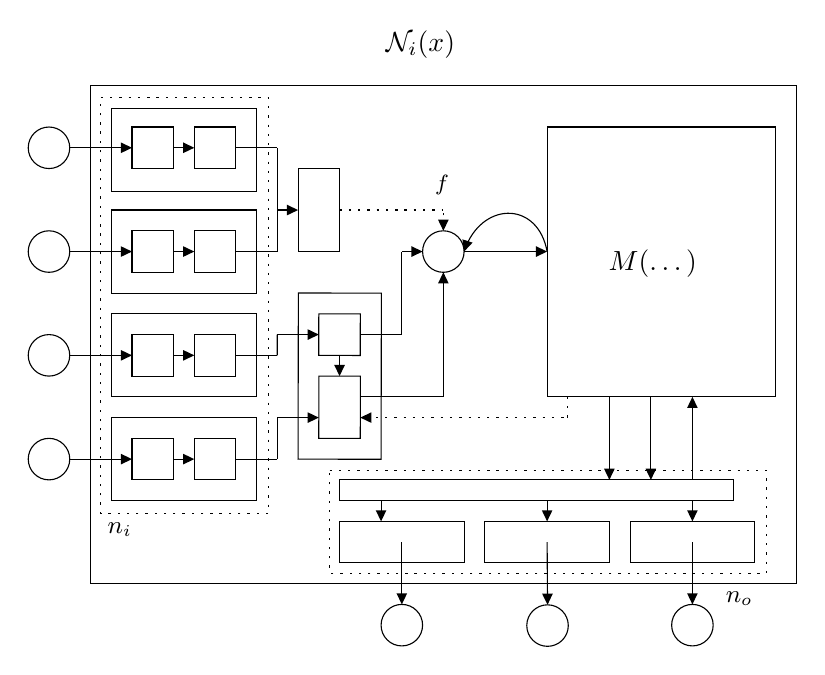
\begin{tikzpicture}[x=0.75pt,y=0.75pt,yscale=-1,xscale=1]
%uncomment if require: \path (0,439); %set diagram left start at 0, and has height of 439

%Shape: Rectangle [id:dp11325550993005518] 
\draw   (100,101) -- (170,101) -- (170,141) -- (100,141) -- cycle ;
%Shape: Rectangle [id:dp0871043429951639] 
\draw   (210,300) -- (270,300) -- (270,320) -- (210,320) -- cycle ;
%Shape: Rectangle [id:dp6243572067188583] 
\draw   (100,250) -- (170,250) -- (170,290) -- (100,290) -- cycle ;
%Shape: Rectangle [id:dp5814395527377063] 
\draw   (100,200) -- (170,200) -- (170,240) -- (100,240) -- cycle ;
%Shape: Rectangle [id:dp8753477258371138] 
\draw   (100,150) -- (170,150) -- (170,190) -- (100,190) -- cycle ;
%Shape: Rectangle [id:dp5798677682795597] 
\draw   (230.15,190.04) -- (230,270.08) -- (190,270) -- (190.15,189.96) -- cycle ;
%Shape: Rectangle [id:dp24707649617836847] 
\draw   (190,130) -- (210,130) -- (210,170) -- (190,170) -- cycle ;
%Shape: Rectangle [id:dp33716600057650536] 
\draw   (350,300) -- (410,300) -- (410,320) -- (350,320) -- cycle ;
%Shape: Rectangle [id:dp9055416056676429] 
\draw   (280,300) -- (340,300) -- (340,320) -- (280,320) -- cycle ;
%Shape: Rectangle [id:dp13764882951656032] 
\draw   (220,200.04) -- (219.96,220.06) -- (199.96,220.02) -- (200,200) -- cycle ;
%Shape: Rectangle [id:dp27863186768492065] 
\draw   (220.04,230.04) -- (219.98,260.02) -- (199.98,259.98) -- (200.04,230) -- cycle ;
%Shape: Rectangle [id:dp5553865711579786] 
\draw   (110,160) -- (130,160) -- (130,180) -- (110,180) -- cycle ;
%Shape: Rectangle [id:dp9842747920805606] 
\draw   (140,160) -- (160,160) -- (160,180) -- (140,180) -- cycle ;
%Shape: Rectangle [id:dp11391650551903476] 
\draw   (110,260) -- (130,260) -- (130,280) -- (110,280) -- cycle ;
%Shape: Rectangle [id:dp09942914368133748] 
\draw   (140,260) -- (160,260) -- (160,280) -- (140,280) -- cycle ;
%Shape: Rectangle [id:dp6297511200807524] 
\draw   (110,210) -- (130,210) -- (130,230) -- (110,230) -- cycle ;
%Shape: Rectangle [id:dp9307891959891459] 
\draw   (140,210) -- (160,210) -- (160,230) -- (140,230) -- cycle ;
%Shape: Rectangle [id:dp8446667441818969] 
\draw   (110,110) -- (130,110) -- (130,130) -- (110,130) -- cycle ;
%Shape: Rectangle [id:dp7846804351453478] 
\draw   (140,110) -- (160,110) -- (160,130) -- (140,130) -- cycle ;
%Straight Lines [id:da5110600464617441] 
\draw    (80,170) -- (107,170) ;
\draw [shift={(110,170)}, rotate = 180] [fill={rgb, 255:red, 0; green, 0; blue, 0 }  ][line width=0.08]  [draw opacity=0] (5.36,-2.57) -- (0,0) -- (5.36,2.57) -- cycle    ;
%Straight Lines [id:da5422700604803716] 
\draw    (80,120) -- (107,120) ;
\draw [shift={(110,120)}, rotate = 180] [fill={rgb, 255:red, 0; green, 0; blue, 0 }  ][line width=0.08]  [draw opacity=0] (5.36,-2.57) -- (0,0) -- (5.36,2.57) -- cycle    ;
%Shape: Rectangle [id:dp9313490804874551] 
\draw   (90,90) -- (430,90) -- (430,330) -- (90,330) -- cycle ;
%Straight Lines [id:da9105070856971889] 
\draw    (80,220) -- (107,220) ;
\draw [shift={(110,220)}, rotate = 180] [fill={rgb, 255:red, 0; green, 0; blue, 0 }  ][line width=0.08]  [draw opacity=0] (5.36,-2.57) -- (0,0) -- (5.36,2.57) -- cycle    ;
%Straight Lines [id:da6609395816932571] 
\draw    (80,270) -- (107,270) ;
\draw [shift={(110,270)}, rotate = 180] [fill={rgb, 255:red, 0; green, 0; blue, 0 }  ][line width=0.08]  [draw opacity=0] (5.36,-2.57) -- (0,0) -- (5.36,2.57) -- cycle    ;
%Straight Lines [id:da0032511945053963487] 
\draw    (130,270) -- (137,270) ;
\draw [shift={(140,270)}, rotate = 180] [fill={rgb, 255:red, 0; green, 0; blue, 0 }  ][line width=0.08]  [draw opacity=0] (5.36,-2.57) -- (0,0) -- (5.36,2.57) -- cycle    ;
%Straight Lines [id:da913878359208306] 
\draw    (130,220) -- (137,220) ;
\draw [shift={(140,220)}, rotate = 180] [fill={rgb, 255:red, 0; green, 0; blue, 0 }  ][line width=0.08]  [draw opacity=0] (5.36,-2.57) -- (0,0) -- (5.36,2.57) -- cycle    ;
%Straight Lines [id:da29849706207756643] 
\draw    (130,170) -- (137,170) ;
\draw [shift={(140,170)}, rotate = 180] [fill={rgb, 255:red, 0; green, 0; blue, 0 }  ][line width=0.08]  [draw opacity=0] (5.36,-2.57) -- (0,0) -- (5.36,2.57) -- cycle    ;
%Straight Lines [id:da5988492285356528] 
\draw    (130,120) -- (137,120) ;
\draw [shift={(140,120)}, rotate = 180] [fill={rgb, 255:red, 0; green, 0; blue, 0 }  ][line width=0.08]  [draw opacity=0] (5.36,-2.57) -- (0,0) -- (5.36,2.57) -- cycle    ;
%Shape: Rectangle [id:dp06329604948993794] 
\draw   (310,110) -- (420,110) -- (420,240) -- (310,240) -- cycle ;
%Flowchart: Connector [id:dp8332863887530595] 
\draw   (250,170) .. controls (250,164.48) and (254.48,160) .. (260,160) .. controls (265.52,160) and (270,164.48) .. (270,170) .. controls (270,175.52) and (265.52,180) .. (260,180) .. controls (254.48,180) and (250,175.52) .. (250,170) -- cycle ;
%Straight Lines [id:da12612212040876503] 
\draw    (160,120) -- (180,120) ;
%Straight Lines [id:da31914662032691554] 
\draw    (180,120) -- (180,150) ;
%Straight Lines [id:da9795534822739309] 
\draw    (180,150) -- (187,150) ;
\draw [shift={(190,150)}, rotate = 180] [fill={rgb, 255:red, 0; green, 0; blue, 0 }  ][line width=0.08]  [draw opacity=0] (5.36,-2.57) -- (0,0) -- (5.36,2.57) -- cycle    ;
%Straight Lines [id:da6816623316052335] 
\draw    (180,150) -- (180,170) ;
%Straight Lines [id:da10214644502871861] 
\draw    (160,170) -- (180,170) ;
%Straight Lines [id:da2333042550366453] 
\draw    (210,220) -- (210,227) ;
\draw [shift={(210,230)}, rotate = 270] [fill={rgb, 255:red, 0; green, 0; blue, 0 }  ][line width=0.08]  [draw opacity=0] (5.36,-2.57) -- (0,0) -- (5.36,2.57) -- cycle    ;
%Straight Lines [id:da6207516705964704] 
\draw    (160,220) -- (180,220) ;
%Straight Lines [id:da8944570569529915] 
\draw    (179.96,220.02) -- (180,210) ;
%Straight Lines [id:da8214897304050846] 
\draw    (180,210) -- (197,210) ;
\draw [shift={(200,210)}, rotate = 180] [fill={rgb, 255:red, 0; green, 0; blue, 0 }  ][line width=0.08]  [draw opacity=0] (5.36,-2.57) -- (0,0) -- (5.36,2.57) -- cycle    ;
%Straight Lines [id:da05957407818008731] 
\draw    (160,270) -- (180,270) ;
%Straight Lines [id:da49398447141544] 
\draw    (180,270) -- (180,250) ;
%Straight Lines [id:da711469323627808] 
\draw    (180,250) -- (197,250) ;
\draw [shift={(200,250)}, rotate = 180] [fill={rgb, 255:red, 0; green, 0; blue, 0 }  ][line width=0.08]  [draw opacity=0] (5.36,-2.57) -- (0,0) -- (5.36,2.57) -- cycle    ;
%Shape: Rectangle [id:dp7948056890037245] 
\draw   (210,280) -- (400,280) -- (400,290) -- (210,290) -- cycle ;
%Straight Lines [id:da8505206798497769] 
\draw  [dash pattern={on 0.84pt off 2.51pt}]  (210,150) -- (260,150) ;
%Straight Lines [id:da9415887071519273] 
\draw  [dash pattern={on 0.84pt off 2.51pt}]  (223,250) -- (320,250) ;
\draw [shift={(220,250)}, rotate = 0] [fill={rgb, 255:red, 0; green, 0; blue, 0 }  ][line width=0.08]  [draw opacity=0] (5.36,-2.57) -- (0,0) -- (5.36,2.57) -- cycle    ;
%Straight Lines [id:da837491588082458] 
\draw    (220,210) -- (240,210) ;
%Straight Lines [id:da06293690723018686] 
\draw    (240,210) -- (240,170) ;
%Straight Lines [id:da7200921856093905] 
\draw    (240,170) -- (247,170) ;
\draw [shift={(250,170)}, rotate = 180] [fill={rgb, 255:red, 0; green, 0; blue, 0 }  ][line width=0.08]  [draw opacity=0] (5.36,-2.57) -- (0,0) -- (5.36,2.57) -- cycle    ;
%Straight Lines [id:da7500647994920802] 
\draw    (220,240) -- (260,240) ;
%Straight Lines [id:da039805258182520564] 
\draw    (260,240) -- (260,183) ;
\draw [shift={(260,180)}, rotate = 90] [fill={rgb, 255:red, 0; green, 0; blue, 0 }  ][line width=0.08]  [draw opacity=0] (5.36,-2.57) -- (0,0) -- (5.36,2.57) -- cycle    ;
%Straight Lines [id:da23764718408033914] 
\draw  [dash pattern={on 0.84pt off 2.51pt}]  (320,240) -- (320,250) ;
%Straight Lines [id:da4687498151820695] 
\draw  [dash pattern={on 0.84pt off 2.51pt}]  (260,157) -- (260,150) ;
\draw [shift={(260,160)}, rotate = 270] [fill={rgb, 255:red, 0; green, 0; blue, 0 }  ][line width=0.08]  [draw opacity=0] (5.36,-2.57) -- (0,0) -- (5.36,2.57) -- cycle    ;
%Straight Lines [id:da24885446056205818] 
\draw    (340,277) -- (340,240) ;
\draw [shift={(340,280)}, rotate = 270] [fill={rgb, 255:red, 0; green, 0; blue, 0 }  ][line width=0.08]  [draw opacity=0] (5.36,-2.57) -- (0,0) -- (5.36,2.57) -- cycle    ;
%Straight Lines [id:da9151151693612134] 
\draw    (360,277) -- (360,240) ;
\draw [shift={(360,280)}, rotate = 270] [fill={rgb, 255:red, 0; green, 0; blue, 0 }  ][line width=0.08]  [draw opacity=0] (5.36,-2.57) -- (0,0) -- (5.36,2.57) -- cycle    ;
%Straight Lines [id:da1416977299387372] 
\draw    (380,280) -- (380,243) ;
\draw [shift={(380,240)}, rotate = 90] [fill={rgb, 255:red, 0; green, 0; blue, 0 }  ][line width=0.08]  [draw opacity=0] (5.36,-2.57) -- (0,0) -- (5.36,2.57) -- cycle    ;
%Straight Lines [id:da36064488959539687] 
\draw    (230,297) -- (230,290) ;
\draw [shift={(230,300)}, rotate = 270] [fill={rgb, 255:red, 0; green, 0; blue, 0 }  ][line width=0.08]  [draw opacity=0] (5.36,-2.57) -- (0,0) -- (5.36,2.57) -- cycle    ;
%Straight Lines [id:da06458094043292584] 
\draw    (310,297) -- (310,290) ;
\draw [shift={(310,300)}, rotate = 270] [fill={rgb, 255:red, 0; green, 0; blue, 0 }  ][line width=0.08]  [draw opacity=0] (5.36,-2.57) -- (0,0) -- (5.36,2.57) -- cycle    ;
%Straight Lines [id:da5371693206109713] 
\draw    (380,297) -- (380,290) ;
\draw [shift={(380,300)}, rotate = 270] [fill={rgb, 255:red, 0; green, 0; blue, 0 }  ][line width=0.08]  [draw opacity=0] (5.36,-2.57) -- (0,0) -- (5.36,2.57) -- cycle    ;
%Straight Lines [id:da14487306050826643] 
\draw    (307,170) -- (270,170) ;
\draw [shift={(310,170)}, rotate = 180] [fill={rgb, 255:red, 0; green, 0; blue, 0 }  ][line width=0.08]  [draw opacity=0] (5.36,-2.57) -- (0,0) -- (5.36,2.57) -- cycle    ;
%Curve Lines [id:da6990479809556309] 
\draw    (271.17,166.88) .. controls (280.24,145.78) and (305.61,146.13) .. (310,170) ;
\draw [shift={(270,170)}, rotate = 287.86] [fill={rgb, 255:red, 0; green, 0; blue, 0 }  ][line width=0.08]  [draw opacity=0] (5.36,-2.57) -- (0,0) -- (5.36,2.57) -- cycle    ;
%Straight Lines [id:da8358677637506173] 
\draw    (240,310) -- (240,337) ;
\draw [shift={(240,340)}, rotate = 270] [fill={rgb, 255:red, 0; green, 0; blue, 0 }  ][line width=0.08]  [draw opacity=0] (5.36,-2.57) -- (0,0) -- (5.36,2.57) -- cycle    ;
%Straight Lines [id:da244617897188945] 
\draw    (310,310) -- (310.18,337.2) ;
\draw [shift={(310.2,340.2)}, rotate = 269.62] [fill={rgb, 255:red, 0; green, 0; blue, 0 }  ][line width=0.08]  [draw opacity=0] (5.36,-2.57) -- (0,0) -- (5.36,2.57) -- cycle    ;
%Straight Lines [id:da5771038762158682] 
\draw    (380,310) -- (380,337) ;
\draw [shift={(380,340)}, rotate = 270] [fill={rgb, 255:red, 0; green, 0; blue, 0 }  ][line width=0.08]  [draw opacity=0] (5.36,-2.57) -- (0,0) -- (5.36,2.57) -- cycle    ;
%Shape: Rectangle [id:dp624674318079391] 
\draw  [dash pattern={on 0.84pt off 2.51pt}] (205.2,275.4) -- (415.8,275.4) -- (415.8,325) -- (205.2,325) -- cycle ;
%Shape: Rectangle [id:dp9005135043880514] 
\draw  [dash pattern={on 0.84pt off 2.51pt}] (95,95.8) -- (175.8,95.8) -- (175.8,296.2) -- (95,296.2) -- cycle ;
%Flowchart: Connector [id:dp5628657474616012] 
\draw   (60,120) .. controls (60,114.48) and (64.48,110) .. (70,110) .. controls (75.52,110) and (80,114.48) .. (80,120) .. controls (80,125.52) and (75.52,130) .. (70,130) .. controls (64.48,130) and (60,125.52) .. (60,120) -- cycle ;
%Flowchart: Connector [id:dp8272773414381507] 
\draw   (60,170) .. controls (60,164.48) and (64.48,160) .. (70,160) .. controls (75.52,160) and (80,164.48) .. (80,170) .. controls (80,175.52) and (75.52,180) .. (70,180) .. controls (64.48,180) and (60,175.52) .. (60,170) -- cycle ;
%Flowchart: Connector [id:dp28635133100043864] 
\draw   (60,220) .. controls (60,214.48) and (64.48,210) .. (70,210) .. controls (75.52,210) and (80,214.48) .. (80,220) .. controls (80,225.52) and (75.52,230) .. (70,230) .. controls (64.48,230) and (60,225.52) .. (60,220) -- cycle ;
%Flowchart: Connector [id:dp25327538239021874] 
\draw   (60,270) .. controls (60,264.48) and (64.48,260) .. (70,260) .. controls (75.52,260) and (80,264.48) .. (80,270) .. controls (80,275.52) and (75.52,280) .. (70,280) .. controls (64.48,280) and (60,275.52) .. (60,270) -- cycle ;
%Flowchart: Connector [id:dp12682149272136733] 
\draw   (230,350) .. controls (230,344.48) and (234.48,340) .. (240,340) .. controls (245.52,340) and (250,344.48) .. (250,350) .. controls (250,355.52) and (245.52,360) .. (240,360) .. controls (234.48,360) and (230,355.52) .. (230,350) -- cycle ;
%Flowchart: Connector [id:dp6810137569820218] 
\draw   (300.2,350.2) .. controls (300.2,344.68) and (304.68,340.2) .. (310.2,340.2) .. controls (315.72,340.2) and (320.2,344.68) .. (320.2,350.2) .. controls (320.2,355.72) and (315.72,360.2) .. (310.2,360.2) .. controls (304.68,360.2) and (300.2,355.72) .. (300.2,350.2) -- cycle ;
%Flowchart: Connector [id:dp01731761461300274] 
\draw   (370,350) .. controls (370,344.48) and (374.48,340) .. (380,340) .. controls (385.52,340) and (390,344.48) .. (390,350) .. controls (390,355.52) and (385.52,360) .. (380,360) .. controls (374.48,360) and (370,355.52) .. (370,350) -- cycle ;

% Text Node
\draw (231,62.4) node [anchor=north west][inner sep=0.75pt]    {$\mathcal{N}_{i}( x)$};
% Text Node
\draw (338.4,167.8) node [anchor=north west][inner sep=0.75pt]    {$M( \dotsc )$};
% Text Node
\draw (394.8,332.6) node [anchor=north west][inner sep=0.75pt]  [font=\small]  {$n_{o}$};
% Text Node
\draw (97,299.6) node [anchor=north west][inner sep=0.75pt]  [font=\small]  {$n_{i}$};
% Text Node
\draw (254.8,131.8) node [anchor=north west][inner sep=0.75pt]  [font=\footnotesize]  {$f$};
\end{tikzpicture}
    }
    \caption{The compound structure construction. The same component can be seen, for $n_i,n_o$ and $M$. Multiple consecutive components construct some components, and further outward. Also, we also reflect the complexity of $\mathcal{C}$ for a given architecture.}
    \label{fig:lalala}
\end{figure}

Hence, we can recursively define neuron, either going up or down, if they satisfy such condition. However, usually, we will only go up, as we will have to define in detail the set $\{ A_{M,i} \}$ of all possible \textit{minimally defined} neuron. \footnote{At this point, I am considering using \textit{group theory} to aid such set compartment.}

There are several assumptions and properties accompanied by this type of neuron structure that we would like to note.
\begin{enumerate}
    \item This neuron structure works \textit{sequentially}. A minimally defined neuron, such as in a practical setting, will have $\mathcal{C}$ to support sequential operation. What this means is present in the definition of the minimal neuron, such that $\mathcal{C} = (\mathbf{w}_{i}, \mathbf{w}_{o}, \mathbf{w}_{M})$, and the operation follows $i \to M \to o$ for an input-process-output session.
    
    \item By extension of the point above, the neuron order in a cluster will also be \textit{fixed}. Usually, this follows a single dimension, or, for example, if there exists a singular span directional vector $\vec{dr}$ that indicates the direction of operation in the cluster.
    
    \item We suppose the \textit{independence} of any components inside a neuron.
    
    \item The neuron is expressed in a \textit{parameterized manner}. That is, the behaviour of the neuron can be expressed, controlled, and designed by modifying and constructing a set of non-realized parameters. If this set of parameters is finite, we say that it is \textit{closed parameterization}. If not—i.e., there can be infinitely many parameters—we call it \textit{open parameterization}.
    
    \item This neuron structure is called the \textit{forgetful neuron}, simply because it works, in principle and in actuality, as a processing unit, in the minimally defined case. We will soon touch upon this definition for the detailed structure of the minimally defined neuron.
\end{enumerate}

When we structure our neuron in this way, it is natural to ask whether the neural unit can be expressed similarly to a \textit{finite automaton} or not. But aside from such an analogy, our minimal neuron is already very powerful. Certain clusters of such neurons, embedded with structure $\mathcal{L}$ of \textit{layer-order clustering} (which can be thought of as a more formal notion for a layered neural network), can approximate any continuous representation scheme $c: \mathcal{X} \to [\cdot, \Sigma]$, given an arbitrary closed interval and to an arbitrary degree of accuracy. We often refer to this as the \textit{universal approximation theorem} for the minimally defined neuron system, and it will serve as one of the focuses of the future analysis.

\subsection{Analysis}
The above construction of the fundamental neuron fundamental create the component model of the minimum processing unit which will be used in various collections of system of related mean. In mathematical modelling context, the neuron model is \textit{descriptive}, meaning that it aims specifically not only for the input-output protocol, but also the unit neuron itself. To do this, we recall any given concrete, functional structure under mathematical formalism is given of the basis, on which abstraction and quantification (without physical realization). Hence, our model here aligns well with such mathematical formalism, in the sense that they end up with abstraction without the impromptu need to signify the inner physical realization - or existence itself. And doing this leaves us with formalizing the \textit{minimally defined neuron} of the class $\mathfrak{N}(\mathcal{N},\mathcal{C})$ into specific requirement. 

The inspiration for the concept of a neuron is a biological one: it stems from the study of the brain or any given processing organs of species with specialized region to be called brain. Considering such, we found out that the brain mostly consists of the fundamental component called biological neuron and its supporting structures - other resource matters of the inner brain that helps to make it function. Without physical realization depends on many things, but most of the time, it is expressed by the proposition that is to remove the physical attachment from any given object of interest, giving it a more quantified look. For a neuron, it can be treated in such way by formalize the neuron component without its supporting structure, replacing electrical signal and other innate signalling mechanism with abstract 'data flow' and 'operations', without much worry about the actual physical realization of chemical reaction and channel - as we do not need such. 

Back there, we all said of the neuron class. What does this mean? For starter, this section on the neuron is the relatively minimal construction we can get it onto. Recall that we say mathematical formalism is to put objects in quantifiable notions, and abstractions of the given subject; also, to express them in a language (or framework, depends on your choice of lexical sense) that support such. Hence, one of the first thing we would like to do, is to formalize the neuron into specific \textit{description scheme}; that is, we would like to treat our objects - the neurons - specifically in certain descriptions that captures the essence of the neural unit, without much ambiguity, and an overhead view of the neuron. The tuple $(\mathcal{N},\mathcal{C})$ did exactly that - it tells us that the neuron is expressed by that separation of descriptions - in the language of mathematical quantification; for then, $\mathcal{N}$ stands for the quantitative \textit{parameters} that characterize the resources, component scale, or the \textbf{mass} of a given neuron, which $\mathcal{C}$ stands for the operations that governs the neuron's internal dynamics. One feasible assumption here is that the neuron does not exhibit any of its operation, that is, interfering with the macroscopic world outside itself, aside from the input-output formalism. Those two descriptions, one governs the mass, one govern the internal mechanics that confounds the subject's behaviours, is what the mathematical description do - and it works very well as it is. 
\vspace{2mm}

In such formalism, $\mathcal{N}$ is typically easier to specify than $\mathcal{C}$ - which is trivial since the internal mechanics is harder to define and construct, for there exists many relationship and connection between components in the same system. And, considering that for any working system, especially for an interactive one, which inherently dependent on the scale $t$, or given any reference point of operation to be referred upon, there can be either infinite configuration, or infinite type of ordering of the system itself. We may come to the analysis on \textit{invariant structure} of the space of configuration, but otherwise, it is uncommon to have invariant structure presented in the majority inside a typical system, except fitting of certain criteria.  

Overall, the neuron formalism of capturing them into a neural class also helps to figure out the \textit{macroscopic configuration} and the \textit{microscopic configuration} of any given neuron. Under a certain instance of the neuron class $\mathfrak{N}$, iterations of individual neurons can be vastly different, depends on their representation scheme $\mathcal{R}$ for individual sub-description of subcomponent - for example, if there exist the component called the \textit{loss function}, then the macroscopic behaviour will only be configured up to certain accuracy, the rest is left for the detail microscopic setting. Hence, we can partition $\mathcal{N}$ into $$\mathcal{N}\supset \mathcal{N}_{\mathcal{H}}(\dots)\times \mathcal{N}_{\mathcal{P}}(\dots), \quad \mathcal{N}_{M}\supset \mathcal{N}_{\mathcal{H},M}(n_{i},n_{o},M)\times \mathcal{N}_{\mathcal{P},M}(n_{i},n_{o},M)$$
of which here we use the word \textit{hyperparameter} for $\mathcal{H}$ a bit different from its usage of literature, and $\mathcal{P}$ for microscopic \textit{parameters}, under the proposition that the properties can be configured using parameters as abstraction. Similar notion goes for $\mathcal{C}$, though it is less apparent. 

Overall, the minimally defined neuron, or what we can take as the \textbf{fundamental model of neural processing unit} works well, and provides us with the first iteration of the constructing brick for our larger, wider implementation. Though our aim is to advance this structure, first, we must take a look to the formalization and propositional-nation of the rudimentary concept of the neuron, even of the fundamental, minimal neuron. And this will happen at the end of this chapter. Until then, examining the maximal usage of the current structure will be more than enough as it aligns with historical literature's neuron and neural network formalism. Following sections will see how far we can go with this. 
\subsection{Why we call it minimal}

It seems a bit weird why we call our construction on its own a \textit{minimal construction}. To see this, though, we have to go back to the definition of a neuron, and the historical viewpoint on the constructing principle. 
%------------------------------------------- PART C. DRAFT -------------------------------------------%
\clearpage
\partepigraph{A man who thinks all the time, has nothing to think except thoughts. Theoretical and philosophical, let the arm raises from the chair and dwindle up the reality that unfolds, for thoughts have no meaning if they are not manifested.}{}
\part{Drafts}
\chapter[Double Descent]{Double Descent}
\section{Note}
This is one of my first research - well, yeah, it started in early 2024, up until now. While there are many things to talk, overall, it is a fairly nice research topic. I wonder where would I go after this research, though, so that is definitely a problem, but for now, I think I will stick to this. When I first encountered this problem, I thought it would be plenty easy. I guess I was wrong, and it might take me more than two years to figure it out on my own at this rate, which is fairly troublesome after all. 

This part of the manuscript contains two parts. The first part is concerned of the \textbf{draft and development notes} during research, and the second part (the one begin with the section abstract), is the \textbf{paper manuscript}. 

\section{Developing analysis}
Okay, before running into the paper itself, uh, what the heck are we talking about? Based off our idea, we are targeting, well, \textbf{statistical learning theory} and the weird problem named \textbf{double descent}. Double descent has its notion from the dilemma of bias-variance tradeoff, a somewhat empirical hack to the problem of model selection. So, what is it? 

\subsection{Statistical learning theory}
Roughly speaking, with machine learning being developed, there are petitions and pushes for the development of a further, more formal ground to explain and interpret the action of learning, and aside from heuristic, empirical design, a somewhat theoretical guarantee net for whatever we will be trying to do. This is where \textbf{learning theory} comes in, with specifically two disciplines - or rather two approaches: \textit{Computational Learning Theory (CoLT)} which applies computational aspect to the learning problem, and the \textit{Statistical Learning Theory (SLT)} which focus on the statistical interpretation of the learning problem. Albeit seems pretty different, they are actually very, well, interconnected, to the point that certain important notions can be almost the same. 

Well, enough speaking by then, we will have the general idea and outward look of a more \textbf{formal system} of analysis. Let's hope we can deal with it. 

\subsection{Double descent} 

Double descent is tricky, in the sense that it is one of those phenomena that you perhaps would say to "break the theory", just like how lights and the Stern-Gerlach experiment broke classical physics' absolute view on determinism. Indeed, the thing that double descent broke is perhaps very important, in our opinion: \textit{the bias-variance tradeoff}. What it means, and how it perhaps is important, we might be able to say. \sidepar{\footnotesize While this sounds perhaps too good, it is indeed, one of the thing that I have to say about it as important.}

Informally, bias-variance is an observation and perhaps analytical derivation of the behaviour of a learning system, within one consideration of the dynamic - complexity versus errors. With machine learning, for correctness reason of the \textit{training session} conducted, error is a requirement. Bias-variance tradeoff connects this with the complexity of the model, by using the two proxies from statistical analysis, called bias and variance (statistical). Their result is pretty much as the following. 

\begin{theorem}[Bias-variance tradeoff]
    For the expected loss of any given hypothesis $h$, the bias $\mathcal{B}(f,y)$ and variance $\mathcal{V}(f,y)$ is inversely proportional, that is, $\mathcal{B}(f,y)\propto \lambda^{-1} \mathcal{V}(f,y)$ for some proportionality $\lambda$ that may or may not be constant. In the most general case possible, $\lambda = -1$ on the entire error range. 
\end{theorem}

We will have to define the notion of the bias $\mathcal{B}$ and the variance $\mathcal{V}$. In the classical derivation of \cite{6797087}, it is defined in a pretty derived way. One can define the bias $\mathcal{B}$ as: 

\begin{equation}
    \mathcal{B}(f,y) = \underbrace{\left\{ \mathbb{E}_{\mathcal{D}}[f(x;\mathcal{D})] - \mathbb{E}[y\mid x] \right\}^{2}}_{\text{bias }}
\end{equation}

and the variance: 
\begin{equation}
    \mathcal{V}(f,y) =\underbrace{\mathbb{E}_{\mathcal{D}} \left\{(f(x;\mathcal{D})- \mathbb{E}_{\mathcal{D}}[f(x;\mathcal{D})])^{2}\right\}}_{\text{variance}}
\end{equation}
Of which both of them are derived from decomposing the supposed test error. 

This results in the ultimate form of the bias-variance curve, which is usually portraited as the following famous inverse graph - there, you can also see the valley of optimality that is the ideal complexity - error ratio that is often wanted. 

\begin{figure}[h!]
    \centering
    \begin{subfigure}{0.4\textwidth}
      \centering
      \includegraphics[width=0.8\textwidth]{img/bias-variance_1.png}
      \caption*{(a)}
    \end{subfigure}
    \hspace{5mm}
    \begin{subfigure}{0.4\textwidth}
      \centering
      \includegraphics[width=1\textwidth]{img/biasvariance_2.png}
      \caption*{(b)}
    \end{subfigure}
    \caption{(a) A typical example of bias-variance tradeoff in a statistical dataset. (b) When graphed into a continuous notion, we gain the complexity-error graph. Notice that it specifically goes for the \textit{test error}, which fits - the representative problem of prediction.}
  \end{figure}
So yes, it is indeed a problem. A very specific one. Especially since it is concerned with one of the main topic of machine learning - model selection. So, what can be said to solve the problem? Historically, not so much. But we will have to eventually take this pill and analyse it historically for now. 

The first identification of the double descent phenomena dated back to the paper of Belkin - \cite{belkin_reconciling_2019}, in which the title is literally "reconciling" modern machine learning practice and the bias-variance tradeoff. What is happening here? In modern machine learning practice, or state-of-the-art developments, models are now bigger than ever. If to notice, we will see that currently models are inherently large, for example, a normal large language model will have from 900 millions (900M) to a few billions, for example 10 billions (10B) parameters. That is not taking into account the overall dynamics and structure of the model, which dictates the operating range and efficiency of the model itself. These model, based on the neural network architecture are somewhat trained to exactly fit (or interpolate) the data, almost certainly so that it turn from a prediction setting to an estimation setting. By statistical learning theory, this would be considered overfitting, and yet, they often obtain very high accuracy on test data. Is the test wrong, or it's just that we are missing something? No one knows for sure. 

\begin{figure}[h!]
    \centering
    \begin{tabular}{cc}
    \includegraphics[height=0.15\textheight]{pdf/u-shaped.pdf} &
    \includegraphics[height=0.15\textheight]{pdf/doubledescent.pdf} \\
    {\bf (a)} & {\bf (b)}
    \end{tabular}
    \caption{{\bf Curves for training risk (dashed line) and test risk (solid line).}
      ({\bf a}) The classical \emph{U-shaped risk curve} arising from the bias-variance trade-off.
      ({\bf b}) The \emph{double descent risk curve}, which incorporates the U-shaped risk curve (i.e., the ``classical'' regime) together with the observed behaviour from using high capacity function classes (i.e., the ``modern'' interpolating regime), separated by the interpolation threshold.
      The predictors to the right of the interpolation threshold have zero training risk. Reproduced from \cite{belkin_reconciling_2019}.}
    \label{fig:double-descent}
  \end{figure}
The main finding that Belkin found is a pattern for how the apparent performance on unseen data depends on model capacity and the mechanism underlying the emergence of double descent. When function class capacity is below the "interpolation threshold", learned predictors exhibit the classical U-shaped curve from Figure~\ref{fig:double-descent}. 
\blockquote[\cite{belkin_reconciling_2019}]{The bottom of the $U$ is achieved at the sweet spot which balances the fit to the training data and the susceptibility to over-fitting:
to the left of the sweet spot, predictors are under-fit, and immediately to the right, predictors are over-fit.
When we increase the function class capacity high enough (e.g., by increasing the number of features or the size of the neural network architecture), the learned predictors achieve (near) perfect fits to the training data---i.e., interpolation.
Although the learned predictors obtained at the interpolation threshold typically have high risk, we show that increasing the function class capacity beyond this point leads to decreasing risk, typically going below the risk achieved at the sweet spot in the ``classical'' regime.}

Belkin tested on several contexts. The first one is with Random Fourier features, in which it is defined as followed. 

\begin{definition}[Random Fourier features]
    The RFF model family $\cHN$ with $N$ (complex-valued) parameters consists of functions $h \colon \R^d \to \mathbb{C}$ of the form
\[
  h(x) = \sum_{k=1}^N a_k \phi(x; v_k)
  \quad\text{where}\quad
  \phi(x; v) := e^{\sqrt{-1} \langle v,x \rangle} ,
\]
and the vectors $v_1,\dotsc,v_N$ are sampled independently of the standard normal distribution in $\R^d$.
(We consider $\cHN$ as a class of real-valued functions with $2N$ real-valued parameters by taking real and imaginary parts separately.)
\end{definition}

This model is evaluated using the formulation of the classical statistical learning theory (refers to the respective chapter, if able), and is tested on the MNIST dataset. Their result? Pretty much the emergence property you observed of the figure above there, in which there exists double descent for both either zero-one loss or squared loss. 

\begin{figure}[h!]
    \centering
    \includegraphics[width=0.8\textwidth]{img/RFFDD.png}
\end{figure}
Another models that they tested is the vanilla neural network, and decision trees and ensemble methods, in which gives you the following shape, similar to their double descent on RFF curve. Notice how a lot of the setting substitute the complexity to be the number of parameters or weight, in which case for decision tree, it is \begin{equation*}
    \mathcal{C}(h_{DT}) = (d+1)\cdot H + (H+1)\cdot K
\end{equation*} 
Which is still quite a lot, for $H$ hidden units, dataset of $K$ classes, and $d$ is the dimension of the MNIST pool channel. 
\begin{figure}[h!]
    \centering
    \includegraphics[width=0.8\textwidth]{img/decisionDD.png}
\end{figure}
\begin{figure}[h!]
    \centering
    \includegraphics[width=0.8\textwidth]{img/DSDD.png}
\end{figure}

For now, perhaps we can see the apparent shape and identification of double descent. Empirically, double descent gives an interpolation point where then the test error `goes downhill' very fast, almost better than the optimal point of the saddle in bias-variance tradeoff. Perhaps this is what happening inside large model, where absolute almost interpolation occurs and then the entire model is, well, so accurate that the test literally imploded. Or is it? 

The second representative paper that analysed double descent, specifically in the setting of deep learning architecture, is \cite{nakkiran_deep_2019}. Here, again, there is the issue with defining the model complexity of the model, and they offered us an understanding using the notion of the \textit{effective model complexity}, $\mathrm{EMC}_{\mathcal{D},\epsilon}(\mathcal{T})$ for a procedure $\mathcal{T}$ with parameters $\epsilon > 0$ and distribution $\mathcal{D}$. 

Another prominent result to look at is \cite{nakkiran_deep_2019}, on the double descent of deep learning models. This is the first step toward identifying double descent to be perhaps, universal. 

But first, we will have to see their beautiful illustration about deep learning's double descent. While being more complex and harder to analyse, they exhibit the same phenomena. Here, we call the region of changing dynamics from bias-variance to double descent relatively to \textit{critical regime}, and the place where the shift happens, is the \textit{interpolation threshold}

\begin{figure}[H]
    \centering
    \includegraphics[width=1.05\textwidth]{img/errorvscomplexity.png}
    \caption{{\bf Left:} Train and test error as a function of model size,
    for ResNet18s of varying width 
    on CIFAR-10 with 15\% label noise.
    %In the under-parameterized regime, test error follows
    %the behavior predicted by classical statistical learning theory, but in the overparameterized regime (once training error is approximately zero),  the test error undergoes a ``second descent'' and decreases as model size increases. The shaded region represents the critically parameterized regime where the transition from under- to over-parameterization occurs. 
    {\bf Right:}
    Test error, shown for varying train epochs.
    %The dashed red line shows that with optimal early stopping double descent is not observed.
    % All models are ResNet18s of varying width,
    % trained on CIFAR10 with 15\% label noise
    All models trained using Adam for 4K epochs.
    %, and plotting means and standard-deviations from 5 trials with random network initialization.
    The largest model (width $64$) corresponds to standard ResNet18. Reproduced from \cite{nakkiran_deep_2019}.
    %    \ptodo{point out that interpolation point for second plot is plotted in the ocean plot}
    }
    \label{fig:errorvscomplexity}
\end{figure}

\begin{figure}[t!]
\centering
\begin{minipage}{.512\textwidth}
  \centering
  \includegraphics[width=1\textwidth]{img/Intro-ocean-test.png}
\end{minipage}%
\begin{minipage}{.488\textwidth}
  \centering
  \includegraphics[width=1\textwidth]{img/Rn-cifar10-p15-adam-aug-train.png}
\end{minipage}
\caption{{\bf Left:} Test error as a function of model size and train epochs. The horizontal line corresponds to model-wise double descent--varying model size while training for as long as possible.
The vertical line corresponds to epoch-wise double descent,
with test error undergoing double-descent as train time increases.
{\bf Right} Train error of the corresponding models.
All models are Resnet18s trained on CIFAR-10 with 15\% label noise,
data-augmentation, and Adam for up to 4K epochs.}
\label{fig:unified}
\end{figure}

In such sense, we cannot seems to filter those figures or data received from the model by itself. Rather, because of such, the team above developed a hypothesis, of which relies on empirical observations at best. 

They define \emph{effective model complexity} of $\mathcal{T}$ (w.r.t. distribution $\mathcal D$) to be the maximum number of samples $n$ on which $\mathcal{T}$ achieves on average $\approx 0$ \emph{training error}. 

\newcommand{\EMC}{\mathrm{EMC}}
\begin{definition}[Effective Model Complexity]
The \emph{Effective Model Complexity} (EMC) of a training procedure $\cT$, with respect to distribution $\cD$ and parameter $\epsilon>0$,
is defined as:
\begin{align*}
    \EMC_{\cD,\eps}(\cT)
    :=  \max \left\{n ~|~ \E_{S \sim \cD^n}[ \mathrm{Error}_S( \cT( S )  ) ] \leq \eps \right\}
    \end{align*}
    where $\mathrm{Error}_S(M)$ is the mean error of model $M$ on train samples $S$.
\end{definition}

Their main hypothesis can be informally stated as follows:

\begin{hypothesis}[Generalized Double Descent hypothesis, informal] \label{hyp:informaldd}
For any natural data distribution $\cD$, neural-network-based training procedure $\cT$, and small $\epsilon>0$,
if we consider the task of predicting labels based on  $n$ samples from $\cD$ then:
\begin{description}
    \item[Under-parameterized regime.]  If~$\EMC_{\cD,\epsilon}(\cT)$ is sufficiently smaller than $n$, any perturbation of $\cT$ that increases its effective complexity will decrease the test error.
    \item[Over-parameterized regime.] If $\EMC_{\cD,\epsilon}(\cT)$ is sufficiently larger than $n$,
    any perturbation of $\cT$ that increases its effective complexity will decrease the test error.
    
    \item[Critically parameterized regime.] If $\EMC_{\cD,\epsilon}(\cT) \approx n$, then
    a perturbation of $\cT$ that increases its effective complexity
    might decrease {\bf or increase} the test error.
\end{description}
\end{hypothesis}

As it turns out, even they themselves do not fully understand such open question, regardless of whatever was stated. 
\begin{quote}
    Hypothesis~\ref{hyp:informaldd} is stated informally
as we are yet to fully understand the behaviour at the critically parameterized regime.
For example, it is an open question what determines the width of the \emph{critical interval}---the interval around the point  in which $\EMC_{\cD,\epsilon}(\cT) = n$, where increasing complexity might hurt performance. Specifically, we lack a formal definition for ``sufficiently smaller'' and ``sufficiently larger''. Another parameter that lacks principled understanding is the choice of $\epsilon$. In our experiments, we use $\epsilon=0.1$ heuristically.

While in both the under-parameterized and over-parameterized regimes increasing complexity helps performance, the dynamics of the learning process seem very different in these two regimes.
For example, in the over-parameterized regime, the gain comes not from classifying more training samples correctly but rather from increasing the confidence for the training samples that have already been correctly classified. 
\end{quote}
So overall, while actually pretty much reproducing results, they did not have a great step forward to the problem.

\section{Issues}

There are plenty issues with the above analysis. 
\subsection{The messiness of analysis}

Truth to be told, the analysis is pretty much \textit{kind of useless}. What I mean by that is despite all the research into it, not much progress has been made in understanding or trying to fix the problem that is there. Instead, it is the same fancy-styled interpretation and re-visualization of the concept by itself, while not asking the underlying question. 

Even more so, it is the issue that \textit{modern practices far outran theory, even classical one}. Furthermore, because of its clearly nature of being a multidisciplinary field, a lot of ideas are poured in from many fields out wide, such that it is very confusing, furthermore, very ambiguous and very informal when working with any of the formal system that analyze the learning system. This gives us the kind of disconnect that we perceived in the theoretical analysis, and the practical aspect of empirical designs and implementations. 

\subsection{The ambiguity of analysis}
Analysis is often, very, very ambiguous. This also includes in the general setting of the experiment itself. Sometimes, even when the issue is with an unknown event like double descent, even the Gaussian white noise is not considered to be a potential factor in the fluctuation. Somehow, it is treated as trivial. Dissecting the system out, ideally there must exist a list of factors and their importance weight according to how the influence the model, yet there seems to be no such insight about that. 

Furthermore, a lot of terms, definitions are often hand-waived in papers or in discussions. This also led to the point that in \cite{nakkiran_deep_2019}, they have to somehow 'reinvent' another type of model complexity itself, albeit unsatisfying of a definition, is still a new kind of definition per insufficiently of such. 

\subsection{Stepping in the wrong direction}

Perhaps we stepped in the wrong direction in most of the analysis and approaches to the problem? For example, are we taking the test error in a wrong way, or the dilemma is actually misunderstood? For example, while it is true that we are taking the test error, with the assumption of unseen data, what happens if the model is actually too flexible to the point that, it can capture almost perfectly the many cases that it is configured, with that substantially big amount of dataset getting in, guarantee it, because of the dataset, an absolute \textit{concept capture} - that is, the true concept space and the observed space is very, very close together that there is simply not a \textit{true unseen data} anymore? 

Perhaps we should review all of it. From statistical learning theory to the interpretation of that itself. We might want to focus on such. 
\subsection{Main problems}
For now, we can identify plenty problems what will have to be resolved during our works on bias-variance tradeoff. 
\begin{itemize}[topsep=1pt,itemsep=0.5pt]
    \item We need to make clear of the phenomena: bias-variance, double descent, the descent action. 
    \item We need a discussion framework that is clear of context for previously arbitrary notion: inductive bias, model complexity, model flexibility, all kind of biases. 
    \item Not only that, but we need also a framework to discuss the disconnect between empirical, practical approach, and a more formal technical ground of studies. 
    \item Experimental setting and understanding. This will require us to develop a scheme to make sense of the complex system in practice, and to explain the empirical observation. Furthermore, we will also have to test the hypothesis that the test error is indeed, wrong of all accord in understanding of the statistical learning theory. 
\end{itemize}
One of the typical problems observed when trying to solve double descent is exactly that - there are too many ambiguities, even in the sense and configuration of the experimental setting, as it adopts scientific research, yet is not well-rounded in their adoption. 
\subsection{Hypothesis}
While it is not perfect, we have several hypothesizes for what to look out for, as well as the formulation needed to interpret certain phenomena and observations. This ranges from topics of re-evaluating the statistical learning theory, estimation and refactor of assumptions (or \textit{inductive bias} when designing models), to different interpretations and representations that can better explain, model, or gives certain insights.  

\begin{enumerate}[label=\arabic*., leftmargin=1.5em, labelsep=0.5em]
    \item Stability of bias-variance measure is questionable, as it is in certain literature, loosely defined by defining a 3-dimensional vector $\lambda=(\lambda_{1},\lambda_{2},\lambda_{3})$ for such: 
    \noindent 
    \begin{equation*}
        \begin{split}
            \mathbb{E}_{\mathcal{D}} \left[d((f,\mathbb{E}[y\mid x])\right] & = \lambda_{1} \mathrm{Bias}(f,y) + \lambda_{2}\mathrm{Var}(f,y)+ \lambda_{3}\epsilon(\mathcal{D})\\ 
            & = \lambda_{1}\underbrace{\left\{ \mathbb{E}_{\mathcal{D}}[f(x;\mathcal{D})] , \mathbb{E}[y\mid x] \right\}}_{\text{bias term}} +\lambda_{2} \underbrace{\mathbb{E}_{\mathcal{D}} \left\{(f(x;\mathcal{D}), \mathbb{E}_{\mathcal{D}}[f(x;\mathcal{D})])\right\}}_{\text{variance term}} +\underbrace{\lambda_{3}\epsilon}_{\text{irreducible error}}
        \end{split}
        \end{equation*}
    where $\epsilon(\mathcal{D})$ is the irreducible error of the system, depends (theoretically) on the intrinsic imperfection of the dataset $\mathcal{D}$. Assessment on stability of such decomposition is recommended. 
    \item We believe that the bias-variance decomposition is a poor estimation and measure for controlling, validating and choosing model from. Specifically, bias and variance term, as well as their supposed expression of decomposition in the standard loss measure of model effectiveness is not representative, nor expressive of the actual, underlying notion of \textit{model complexity} $C(f)$ and its effectiveness. Furthermore, bias-variance decomposition is not straight-forward of others type of loss functions, except only for some classes of loss function (loss on Bregman divergences and exponential class). 
    \item Inductive bias obviously plays a role, as mentioned by some literature \footnote{Need to include some in here.}, though we don't know exactly how the inductive bias can be formed to play any role in the central dynamic of the model operating process. Certain assumption, for example, the \textit{convexity of the loss function} might actually affect the model as it is, and introduce unwanted patterns in the following process. 
    \item Random initialization of parameters, as well as the initial conditions of the model initialization process might also be taken into account. Obviously, this is not a new insight, and is rather a very old one, however, this approach still have varied potential for interpreting double descent. Scaling up/down this effect might result in new insight, as well as inspecting the uncertainty and diffusion patterns in large-scale model deployment, in which from an end-to-end perspective requires several space transformation operations in successions.
    \item The PAC-learning framework, and its generaliy to \textit{agnostic PAC-learning}, seperate the concept class $c$ into two individual parts - either the assumption $c\in \mathcal{C}$ is true, or $\mathcal{C}$ is absent in the hypothesis, and therefore the inductive bias (assumption priori) is reduced of the underlying concept. However, most of the assumption and sepration comes around in the generalization is by assuming $\mathcal{X}$ is also random, and therefore unpredictable by the most random scenario. The most common justification of the generality of agnostic case, is by considering a non-unique nature of the input space's labels. However, usually, there is no assumption or any justification that species that the label, or the target class (of painter) must be \textit{unique}. In fact, of the measure in binary classification, for $\mathcal{Y}=\{0,1\}$, used in \cite{10.5555/2371238} for PAC-learning class, it is indeed a case of repeating label. The reason for this separation then is ambiguous and not totally founded. Though, it is reasonable to assume $\mathcal{X}$ is embedded with random probability, by separating the concept similar to what is illustrated in \ref{fig:PhaseDiagram}, there exists a distinct \textit{internal relation}, for example, the probabilistic constraint of the input space $\mathcal{X}, p(X)$ unaccounted for $c$. However, grouping $c$ by justifying properties of $\mathcal{X}$ is not so good. For example, consider $c$ to be an automaton, either finite state automaton, or infinite state automaton (pushdown machine, Turing machine). Either $c$ can be considered \textit{deterministic} or, \textit{non-deterministic} - for example, Probabilistic Turing machine (PTM), where state transition is justified of certain propabilistic measure embedded. Assuming so, we can see that probability, if exists in such automaton, will only be defined upon the pair $(c,\mathcal{Y})$, and not $(\mathcal{X},c)$ - the \textit{ground space} (input) has no justification on $c$ if specifically so.  
    \item The very ambiguous idea or treatment of statistical learning, as well as machine learning, is the idea of masked. Or, paraphrased, \textit{hidden information} regarding the underlying process of estimation. Specifically, for example, we tend to assume things to not be able to grasp - either the probability $p_{X}(c)$ of the concept class, the distribution $\mathcal{D}$ specified to such input distribution, or the concept class $\mathcal{C}$, Markov properties, etc. We would like to formalize this notion as soon and as such in the most direct way. 
    \item The most outlandish one is that the test error is actually, to be seen as falsely interpreted by statistical learning theorists. 
\end{enumerate}

We cannot answer nor verify every single bit of the above hypothesis. However, by listing so gives us certain insight in which can be potentially refuted or agreed upon, it will base our understanding of the system in a more clear sight. 

We have one more hypothesis on implementation. 

\begin{itemize}[noitemsep,topsep=0.5pt]
    \item As we have seen with the disparity between SVM and other parameter-wise complexity measure, it is then to see that the measure of complexity is extremely lacking. It is also observed that many attempts has been made to categorize different types of complexity for a given model. It is then suggested, would there exists an algorithm or at least a behavioural control method that find the optimal, weighted complexity measure analysis? That is, assuming we have all the currently available complexity measure that we can find, then because we don't know what to consider "better" than the others, if we just simply weight them on, then tune the parameters of such tuning, then will we have a figuratively confident results that is applicable to a wide range of model selection procedure in such sense? 
\end{itemize}

\subsection{A rather simple solution}

It can perhaps, be observed, that our entire description of the machine learning problem is informal and often not well-organized. Of course, in the face of progress little can be spared toward making things clean. After all, it is the pioneers who plunder and conquer distant lands. However, in the case of our machine learning research, it leaves a wide gap in the analysis and any potential solution at present, to some of the more meticulously difficult and obscure problems of the consequences of such rapid development, for example, our double descent. One of which is the consideration of the \textit{system transparency problem}. 

We may want to expand our notion of the mathematical modelling statements. A \textbf{mathematical modelling setting} consists of, consequently, three simplified components $(S,Q,M)$. $S$ contains the system and its object of interest, $Q$ set up the problem aims, and $M$ acts as information, assumptions, and constraints of the setting. Usually, even under such consideration, the problem setting is treated as an external source - an isolated system $S$ of which contains the subject of interest \textit{only}, and the model, on either extreme of being phenomenological or mechanistic. However, unknowingly, the aspect in which machine learning and subsequently deep learning, or any form of automating correlation known as \textbf{learning}, is doing things differently. 

It is then theorized of a simple configuration. We extend $S$ to encompass the entire hypothesis by itself. Though it is rather strange to do it in a formal sense, less of the cumbersome task for which it seems that we have already conducted. However, even if such line of argument is right, we have indeed, not configured our system accordingly. This is presentable in even the book \cite{VeltenetalMathematicalModelling}, in which we treat the phenomenological model (neural network at foremost) only as an outer method. This is then recognized, for the time being of the hypothesis, to be an insufficient conduct. 

It turns out, however, we can think of our models to be subsequently realizing the internal mechanics by its own representation. As for the rather arbitrary definition of phenomenological and mechanistic model, it can be clearly seen: overall, those models differ only in their configurations of being either totally blind, or are given any sense of the underlying internal structure's interpretation of the events - factors and degree of freedoms, parameters and constants setting. Under multiple extreme assumptions, the notion of \textbf{transparency}, for if it is said that the problem is entirely exposed of its mechanics, or is totally unknown, is considered. Machine learning, and the learning action generally, would play as to mimic the mechanics by itself, regardless of internal mechanics transparency, by its own \textit{representation} as we have been speaking of, with the condition that the acting space remains the same. This is partially guaranteed by the reduction of the observation space into an input-output channel observations. It is then, to be seen, if we can conjecture that any problem setting in transition to mathematical formalism, that is, including the act of observing, recording, and else that gives the dataset by itself, can be reduced nominally to various unknown, arbitrary, primitive parameters and of-no-knowledge models. With such, even differential equations can be somewhat observed, given the right representation space and enough encoding. 

Why is this not so prominent then, in a more classical machine learning setting. It partially has something to do with the relative way both classical machine learning and deep learning are constructed, or rather, the structural constraints between the two. While indeed, such problems would be encountered in classical ML, the design of such models are rather intrinsically different, in the sense that they are restricted and of not so fluid form. Furthermore, they are also specialized, for example, in the original text of \cite{Vapnik1999-VAPTNO}, to works on pattern recognitions, regression problems or density estimation. Such tasks are fairly limited and constrained of their setting and requirements, hence, nominally, the class of "pretty good and extraordinarily useful" model structures are also constrained small enough for the representation to be in classical form; and, given that the learning setting is often not so rigorous as many aspects were not linked together, it puts a fair strain onto such interpretation. 

This is where we would theorize our idea. Rather than just as classical machine learning indicted, from certain observations of \textit{neural network}, it can be said that the following conjecture will be stated. 

\begin{conjecture}
    The learning problem can be considered a one-way description-representation learning problem between the concept structure $\mathcal{C}$ and the hypothesis $\mathcal{H}$. \footnote{The structure and the underlying observations, plus information exchanges, are typically formed into input-output interpretation.}
\end{conjecture}
\begin{conjecture}
    Under deep learning structure, one assumes that every possible configuration and representation of certain concept $c\in \mathcal{C}$ can be decomposed to the standard representation components. 
\end{conjecture}
It is then to see if such conjecture can be observed, or at least proved heuristically. Aside from this conceptual perspective, we also note that in most of its conception, the testing and theoretical working of the theory indeed also is based on the notion of transparency - for example, Agnostic PAC-learning where we assume no knowledge is possible about the class $\mathcal{C}$ of all concept class conceivable of the problem. Such assumption is the transparency window that we are talking about. Rather than doing experiments without considering such, it is then wised to perhaps analyze, how, we can reconstruct the setting, using an end-to-end (only the supervisor or the designer - we - know) phenomenological$\to$ mechanistic learning behaviours occurs. This also perhaps will outline a controlled environment in testing out information theory and interpretation of KL-divergence. 

\section{The perspective of modelling theory}

A normal configuration of a mathematical modelling system, in which the language of mathematic is applied, often consists of three components: The system $S$ in which all the objects, the landscape, the resources, the parts that is considered lives in; The question, or the \textbf{objective} that is of interest, this is also called the setting, or the scenario in which the system is placed in, of a specific notion; and the statements $M$ of which assumptions, statements, condition, restrictions are put on for the system, though not necessary so for the objective. Then, for every model and the construct that we want to make, we have to then specify those first, in the most rigorous manner possible, to disparage the ambiguity. This starts by, as the name of the section called, specifying and constructing the system $S$. 

Before we continue, it is to note that these are some of the more \textbf{informal treatment} of the research direction. Later on, we will have to find something, or some mathematics to tackle the problem laid down here. 

In a typical system $S$ of machine learning, we assume there exists the following objects: 

\begin{itemize}[topsep=1pt,itemsep=0.5pt]
    \item The \textbf{concept object}, which is implicitly the object of study. This object has its own mathematical construct. 
    \item The \textbf{hypothesis object}, which implicitly is the object in which objective is to study the concept object. Similarly, it has its own mathematical construct. 
    \item The \textbf{evolutionary object}, which it aims to correct the hypothesis object to align with the concept object. 
\end{itemize}
Those two first objects have their own mathematical construct, and live in a space in which we call the ground space, of which all their operation and behaviours will be observed. Here, we have the consideration of their \textit{transparency}, that is, the amount of information we know about the object. Or rather, it is called the relative \textit{priori knowledge} about each of them. Using this, we have \textbf{absolute black-box} - where the object is believed to only be an input-output process, without any priori about what is the underlying structure, ever. On the other hand, we have \textbf{total transparency}, in which the internal mechanics of the system is totally clear with respect to the object participated in the dynamic of the object. Before that, let's look at the structures of the two first important object. 
\subsection{Structures of object}


Each object in this system would then have to have a very important component: its \textbf{representation}. This is trivial of interest, because as we said, mathematical modelling convert something into the mathematical formalism and language. In the case of learning a mathematical object by itself, there are also multiple interpretations, definitions, and representation of different objects in different cases, however, most of the time, we will observe a lot of object with very explicit representation of a class of itself. This relies on, for the reason to specify representation, the notion of \textbf{operable object} by itself. An object is \textit{operable} if its internal structure and its nested substructures is arranged, organized, and represented such that there exists operators on which is specified as the action of the object. For example, a function is operable since its substructure includes sub-objects that are the blobs of parameters and the free-variable parameter $b$ (as people always call it such), of which the operations and relations between them constructs to be an operable object by virtue of its observable being produced. For a graph, however, it is inherently static - its structure does not provide us with any actionable quality or operation. Only by either a walk or a trail (which essentially the same thing). To provide or extract the object's structure in an effective sense, which can be said of to not just copy the entire graph, we need to have actions and operations that defines on the graph, to extract meaningful data from it. This is perhaps relevant of the neighbourhood aggregation in a GNN (graph neural network), as it too, needs to extract data by using neighbourhood properties. The graph itself is not equipped of any operable structure. So there is it. 

The next component about an object in our consideration, is the utilization of the representation scheme to then make the class of all descriptions by itself. For example, a representation scheme consists of multiple neuron components - the parameters of each neuron, the path given, et cetera, will only be effective and useful if it is constructed in a structure by itself, that is, in a neural network architecture where neurons are composed of some of those parameters or resources given, with their value based on the field specified in the notation of a numerically-realized representation scheme. This will mostly be the more important notion of the description of the object, since it is where certain criteria, conditions, restrictions and overall description of the object is specified, using the restricted language of the representation scheme. We will see how this is done. 

\subsubsection{Representation}
Then, what can be said about the representation of the hypothesis and the concept objects? Okay, this is harder than I thought. There are many ways to represent a structure or a concept of interest, yet, we will stick to this one, maybe. We will stick to the one that is most familiar: remember in mathematics where we have \textit{sets} embedded with structures? Yeah, about that\dots we will do the same thing. The representation that is used to represent our structure will be called the \textbf{representation scheme}. 

First, we have the following assumption, which will fall to the set of statements $M$, that is as followed. 

\begin{assume}
    The hypothesis and the concept are both represented in the same representation scheme. 
\end{assume}
If the concept is not of the same representation scheme as the hypothesis, then there must be a \textbf{representation encoder} to handle such task. Depends on the restriction of the representation, we can figure out the total loss of information, generality of information in-between such encoding. We define the concept of the representation scheme as followed. 
\begin{definition}[Representation scheme]
    For a system and its object, an object's \textbf{representation scheme} $\bm{\mathcal{R}}$ is a function $\bm{\mathcal{R}}: (\Sigma\cup \mathcal{G})^{*}\to \mathcal{O}$, where $\Sigma$ is the operator alphabet, or relational structure, $\mathcal{G}$ are the components, and $\mathcal{O}$ is the object. $(\Sigma \cup \mathcal{O})^{*}$ is the coupling of \textbf{all} configuration of the components and the operators. 
\end{definition}

In case where scalar numbers are presented, for example, in the axis-aligned rectangle case, we will have: $\bm{\mathcal{R}}^{2}_{\square}:(\Sigma\cup \mathcal{G}\cup\mathbb{F})^{*}\to \mathsf{Rec}$ of all rectangle using this representation scheme, so 
    \begin{equation}
        \bm{\mathcal{R}}_{\square} = \begin{cases}
            \Sigma = \{\leq, \land \}\\
            \mathcal{G} = \{l_{c}, p_{c}, a\}\\
            \mathbb{F} = \mathbb{R}
        \end{cases}
    \end{equation}
    For the formula of all concepts $c$ being axis-aligned rectangle as: 
    \begin{equation}
        \sigma = \{c\} = \bm{\mathcal{R}}^{2} = \{a(x_{a},y_{a}) \mid l_{c}^{(1)} \leq x_{a}\leq p_{c}^{(1)}\land l_{c}^{(2} \leq x_{y}\leq p_{c}^{(2)}\}
    \end{equation}
    Generally, this is called the \textit{numerical representation scheme}, in which it is supported by a field (we do not care much about the dimension of the field, as long as we can decompose it to discrete scalar taking values), that is, $\bm{\mathcal{R}}:(\Sigma \cup \mathcal{G}\cup \mathcal{F})\to \mathcal{O}$. Any representation specification $\sigma\in (\Sigma \cup \mathcal{G}\cup \mathcal{F})$ such that $\bcal{R}(\sigma) = c$ is a representation of $c$ on $\bcal{R}$, denoted $\sigma_{c}$, and the set of all such specification $R_{c}=\{\sigma_{c}\}$ is called the \textbf{representation space} of $c$ on $\bcal{R}$.
    
    The set of all hypotheses $h$ that is specified by certain representation scheme $\bm{\mathcal{R}}_{h}$ is called the \textbf{hypothesis class} $\mathcal{H}$, and $\bm{\mathcal{R}}_{h}$ is the \textbf{hypothesis class representation}. Similarly, for a concept $c$ the set of all concepts that are represented by $\bm{\mathcal{R}}_{c}$ is called the \textbf{concept class} $\mathcal{C}$ for the \textbf{concept representation scheme} $\bm{\mathcal{R}}_{c}$. 

The necessity of the description of a field is rather natural, especially since we are working on a numerical encoding. Generally speaking, the computer at large represents a very complex binary encoding of numerical logical operations, though via abstractions, most of them are 'cancelled out' of the fundamental details. We can almost make a \textit{representation space} just similar to how we define vector space, though, it is more or less not so effective as it can. 

Using this, we can specify \textbf{a lot} of object class. The first one though, we can specify the representation scheme of an input-output model. Now, for this type of definition, then the class of all \textbf{linear function representation} can be designed as 
\begin{equation}
    \bm{\mathcal{R}}_{L}^{n} = \left\{ \{x_{1},\dots,x_{n}\}, y \Bigg| \sum_{i=1}^{n}w_{i}x_{i} + b \land w_{i}, x_{i}, b \in \mathbb{R} \right\}
\end{equation}
From this, we can notice that there exists the notion of \textit{size} for the object class. In one way or another, we have abstracted of the class of all objects that can be specified in such a way that their representation falls into the range of such representation class. Then, we might want to consider the concept of a \textbf{representation complexity}, and the size of the class, denoted $size(\bm{\mathcal{R}})$. Do note that this is not defining the operational complexity, but simply the structure by itself. Which is why we might want to have the definition of an object in such system that we are considering.

Two representations $\bcal{R}_{A}$ and $\mathcal{R}_{B}$, they are said to be \textbf{equivalent} if one can convert objects from the first representation to the second one, and vice versa. Then two representations are said to be \textbf{equal} if their size is the same, assume that the representation scheme is equivalent. This prompts us to define the notion of the size of the representation, but before that, a general insight will be the follow through - you have to be able to reduce one to the others, and reverse. By then, essentially, \textit{you cannot compare apple to orange}, that is. Generally, the size of a representation class is defined the smallest representation of the object in the underlying representation. So, for your example of the linear function, then 
\begin{equation}
    size(c)=\min_{\sigma \in R_{c}}\{size(\sigma)\}
\end{equation}
which again, prompt us \textit{again}, to figure out the notion for $size(\sigma)$. Before then, and defining the object's descriptions, let's try to construct a few more 'mathematical construct' of the same type. A subtle remark can be made here, that the representation only, again, specify the parameters used to represent it, and the string accompanied by such representation. The overall total repetition, for example, of a certain variable, and operation succeedingly, is totally irrelevant. I just get the formula as a shorthand for that scheme up there, as it is. Which again, means that to specify it, you need both the components and how it is connected. Abstractly speaking, and generally speaking. 

\begin{note}
    It is sufficient to note here that the representation scheme has its complexity more than just the count of all its subsequent operations. for example, if the class of the multiplication operation is included, it will, of course, drastically change the dynamic and presentation of the encoding possible for the description. If so, then, we have a very hard time in the future to try "ranking" these type of operators together. Furthermore, while not of the representation complexity itself, the combination of the components in the description also decides another type of complexity, which for now maybe we will call as \textit{expression complexity}. 
\end{note}

Do note that even though the representation scheme is inherently denoted similar to an end-to-end formula would look like, it is not the case, usually. The representation scheme is not a fully mathematical-defined object, for such case then the object itself would have no meaning at all. In such sense, one can define a representation scheme that contains intricate operating structures instead, for example, a self-loop network with various potential-like mechanism and affectants. 


Overall, the role of the representation is to specify the arbitrary language of working. While we are not taking the more diluted problem between the translation from physical, real setting to the mathematical world, and restrict ourselves to the part of which arbitrary mathematical settings take place, it is still of importance of the \textit{language of mechanism} that underlies the structure of certain system pertaining to actions and modelling  \footnote{This way of doing things are particularly similar to a philosophical mathematics's way of defining mathematics through axiomatizations: first they also have to define the symbols and the symbolism expression, as well as the descriptions of mathematical objects through such axiomatization and symbol conventions. This is why some branches of mathematics, where they pertain on a general notion like \textit{set} and \textit{logic} formalism, is used far wider than their own - the language of something like \textit{set theory}, \textit{category theory}, and \textit{logic} are much more useful in other fields or others mathematical objects in which its general framework can be applied to express distinct and more specialized, descriptive objects.}. By doing so, it encompasses a variety of mathematical descriptions in which expresses a very similar aspect of the mathematical language, the configuration and largely operative nature of an object-dependent setting. While doing so, it also makes way for the more in-focus notion of \textit{descriptions} to be defined, and such way encompass a lot of structures, for example, the binary class descriptions of a typical computer, for example. We shall examine this later, for its implications large.

\begin{figure}[h!]
    \centering
    \includegraphics[width=0.6\textwidth]{img/representation_description_scheme.png}
    \caption{The representative order of representation and description. As of the name implied, in transition to a mathematical formalism and language, there must then exist a representation to each and every element of certain subject. The process of doing is this called \textit{external encoding}, and is true also between portion of mathematical-encoded system to each other, if they are distinct. The reverse act is called again, \textit{decoding}, and between mathematical subjects to each other might as well be called \textit{internal encoding}, with respect to the mathematical language.}
\end{figure}

Hence, from the definition and consideration of the representation space, we can at least organize and capture the: 

\begin{enumerate}[topsep=1pt,itemsep=0.5pt]
    \item Representation language: What type of language are considered and how to specify its component, at least in the operational sense of what we are dealing with. 
    \item Representation complexity: While the notion of \textit{complexity} is inherently complex, it is still applicable of current knowledge to then approach the problem of \textit{representation complexity}. This can be done by \textit{representation infimum} and \textit{representation supremum}, both of which will bounds the representation size as much as it could, except for representation anomalies. 
    \item The relative dynamic between \textit{representation complexity} and \textit{representation computational complexity}: In the subject of efficiency in working with representation, it also between computational cost and the richness of the representation space that is of interest. In which, we should encounter, and try to process. 
\end{enumerate}

We would likely want to give a pretty much different interpretation thereof, on one of the more primitive notion in mathematical analysis, which also looks just as similar in idea as the representation of subject to be: the \textbf{Stone-Weierstrass Approximation Theorem}, which states that for $f\in C([a,b],\mathbb{R})$, then there is a sequence of polynomials $p_{n}(x)$ that conveys uniformly to $f(x)$ to $[a,b]$, essentially represents the complex subject. We would ultimately, in actuality, assume this to be true in our connection to practical problems and more complex subjects non-mathematically, and if this is not particularly true, then we are in plenty of trouble. 

\subsubsection{Description}

While the representation space is helpful, it does not capture the entirety of the analysis as a whole. More specifically, it only specify at most the structure of the bricks laying the object, not the object itself. 

Using such alphabet, we then can construct various structures of interest. 

\section{The perspective of modified learning setting}



\clearpage

\section{Bias-variance: A history}
While a lot is known about bias-variance tradeoff, its history is pretty much indeterminate in the lens of a contriving analysis. Rather, controversies and theoretical development that have led to the appearance of double descent, and other phenomena like grokking and else, is of particular chaotic picture in the wider scene of the learning theory, especially of modern time learning. The original definition of bias-variance tradeoff by \cite{6797087} is first constructed using the means-square error, which is regarded as a normal measure in the real encoding space. Their approach is to justify bias-variance via decomposition of the loss function $\ell$, for such to find an alternative reasonable form of such loss landscape. We will eventually notice a lot of the assumptions, and the breakdown of the nominal setting hidden inside this portion of subject matter.

Suppose of a regression problem to construct a hypothesis function $f(x)$ from $(x_{1},y_{1},\dots,x_{N},y_{N})$ for the purpose of generalization - that is, predicting unseen variational values for different pair $(x_{j}, \mathord{?})$ such that $\mathord{?}=y_{j}+\epsilon$ for a conceivable implicit error. To be explicit about the relation of this problem, or $f$ on the given data $\mathcal{D}=\{(x_i, y_i)\mid i \leq N\}$, denote $f(x;\mathcal{D})$ instead of $f$, the natural mean-square measure as a predictor is: 
\begin{equation}
    \mathcal{M}(f,y) = \mathbb{E} \left[((y-f(x;\mathcal{D})))^{2}\mid x, \mathcal{D}\right] 
\end{equation} for $\mathbb{E}[\cdot]$ the expectation wrt to a distribution $P$. Decomposing the right-hand side, we have: 
\begin{equation}
    \mathcal{M}(f,y) = \mathbb{E} \left[((y-f(x;\mathcal{D})))^{2}\mid x, \mathcal{D}\right] = \mathbb{E}\left[(y-\mathbb{E}[y\mid x])^{2}\mid x,\mathcal{D}\right] + (f(x;\mathcal{D})-\mathbb{E}[y\mid x])^{2}
\end{equation}
Here, $\mathbb{E}\left[(y-\mathbb{E}[y\mid x])^{2}\mid x,\mathcal{D}\right]$ does not depend on $\mathcal{D}$, but simply the statistical variance of $y$ given $x$. The term $(f(x;\mathcal{D})-\mathbb{E}[y\mid x])^{2}$ is considered a natural measure of effectiveness on $\mathbb{R}^{n}$ as a singular predictor of $y$. Now, for $\mathbb{E}_{\mathcal{D}}\left[(f(x;\mathcal{D})-\mathbb{E}[y\mid x])^{2}\right]$ which depends on the training set $\mathcal{D}$ in its computation, is decomposed into the form of \textit{bias-variance decomposition} terms, by derivation: 
\begin{equation}
    \begin{split}
        \mathbb{E}_{\mathcal{D}} \left[(f(x;\mathcal{D})-\mathbb{E}[y\mid x])^{2}\right] & = \underbrace{\left\{ \mathbb{E}_{\mathcal{D}}[f(x;\mathcal{D})] - \mathbb{E}[y\mid x] \right\}}_{\text{bias term}} + \underbrace{\mathbb{E}_{\mathcal{D}} \left\{(f(x;\mathcal{D})- \mathbb{E}_{\mathcal{D}}[f(x;\mathcal{D})])^{2}\right\}}_{\text{variance term}}
    \end{split}
\end{equation}

We summarize this in the following statement. 

\begin{theorem}[Bias-variance tradeoff]
    Suppsoe the model $f(x;\mathcal{D})$ for the data $\mathcal{D}=(x_i, y_i)$ and its parameter $x$ is defined. For $y_{i}$ of the target concept's responses $y$, and consider a regression problem with the loss measure $\mathcal{M}(f,y)$ of mean squared risk, the following statement is true: \begin{equation}
        \mathbb{E}\big[\mathcal{M}(f,y)\big] = \mathcal{B}(f,y) + \mathcal{V}(f,y) + \mathbb{E}\Big[\mathbb{E} \left[((y-f(x;\mathcal{D})))^{2}\mid x, \mathcal{D}\right]\Big]
    \end{equation}
    for $\mathbb{E}[\:\cdot\mid x, \mathcal{D}]$ any expression with dependencies on $x$ and $\mathcal{D}$. The bias and variance term is subsequently expressed by 
    \begin{align}
        \mathcal{B}(f,y) = \underbrace{\left\{ \mathbb{E}_{\mathcal{D}}[f(x;\mathcal{D})] - \mathbb{E}[y\mid x] \right\}}_{\text{bias }}, \quad \mathcal{V}(f,y) =\underbrace{\mathbb{E}_{\mathcal{D}} \left\{(f(x;\mathcal{D})- \mathbb{E}_{\mathcal{D}}[f(x;\mathcal{D})])^{2}\right\}}_{\text{variance}}
    \end{align}
\end{theorem}

\begin{proof}
    We present the original derivation of bias-variance tradeoff and its analysis from \cite{6797087}. Geman's paper is, by his own word, concerned of \textit{parametric models}, i.e. hypothesis class without strong assumption of parameters defined, though the definition of bias-variance tradeoff afterward and its justification is made in the sense of parametric model. We partially clarify\footnote{Generally, there is no definite definition on what would be considered non-parametric. Though, an example might be drawn from the (vanilla) neural network and Gaussian Process Regression (GPR)} this with the following definition as customary. 

    \begin{definition}[Parameterization]
        A \textbf{parametric model} is one that can be parameterized by a fintie number of parameters. In general, for a hypothesis class $\mathcal{H}$of all parametric hypothesis is then expressed as:
        \begin{equation}
            \mathcal{H} = \{f(x;\theta): \theta \in \Theta \subset \mathbb{R}^{d}\}
        \end{equation} where $\Theta$ is called the \textit{parameter space}. A \textbf{nonparametric model} is one which cannot be parameterized by a fix number of parameters.   
    \end{definition}
    Suppose of a training dataset $\mathcal{D}$ of $N$ 2-tuples $(\mathbf{x}_{i},y_{i})$, that is: \begin{equation}
        \mathcal{D} = \{(\mathbf{x}_{1},y_{1}),\dots,(\mathbf{x}_{N},y_{N})\} \quad \lvert \mathcal{D} \rvert = N, \mathbf{x}\in \mathbb{R}^{d}, y \in \mathbb{R}
    \end{equation}
    The regression problem is to construct a function $f(\mathbf{x})\to y$ based on $\mathcal{D}$, which is denoted $f(\mathbf{x};\mathcal{D})$ to show this dependency. Then, 
    \begin{equation}
        \begin{split}
            \mathbb{E}\left[ (y-f(\mathbf{x};\mathcal{D}))^{2}\mid \mathbf{x},\mathcal{D}\right] & = \mathbb{E}\Big[\big( (y-\mathbb{E}[y\mid \mathbf{x}]+ (\mathbb{E}[y\mid \mathbf{x}]-f(\mathbf{x};\mathcal{D}))) \big)^{2}\mid \mathbf{x},\mathcal{D}\Big]\\
            & = \begin{multlined}
                \mathbb{E} \Big[ (y- \mathbb{E}[y\mid \mathbf{x}])^{2}\mid \mathbf{x},\mathcal{D} \Big] + \Big(\mathbb{E}[y\mid \mathbf{x}-f(\mathbf{x};\mathcal{D})]\Big)^{2} \\ + 2\mathbb{E} \big[(y-\mathbb{E}[y\mid \mathbf{x}])\mid \mathbf{x},\mathcal{D}\big]\cdot \big(\mathbb{E}[y\mid \mathbf{x}]-f(\mathbf{x;\mathcal{D}})\big)^{2} 
            \end{multlined} \\
            & = \mathbb{E} \Big[(y-\mathbb{E}[y\mid \mathbf{x}])\mid \mathbf{x},\mathcal{D}\Big] + \big(\mathbb{E}[y\mid \mathbf{x}]-f(\mathbf{x};\mathcal{D})\big)^{2}\\
            & \geq \mathbb{E} \big[(y-\mathbb{E}[y\mid \mathbf{x}])^{2}\mid \mathbf{x},\mathcal{D}\big]
        \end{split}
    \end{equation}
    Hence, we decompose it to: 
    \begin{equation}
        \mathbb{E} \left[((y-f(\mathbf{x};\mathcal{D})))^{2}\mid \mathbf{x}, \mathcal{D}\right] = \mathbb{E}\left[(y-\mathbb{E}[y\mid \mathbf{x}])^{2}\mid \mathbf{x},\mathcal{D}\right] + (f(\mathbf{x};\mathcal{D})-\mathbb{E}[y\mid \mathbf{x}])^{2}
    \end{equation}
    Where $\mathbb{E}\left[(y-\mathbb{E}[y\mid \mathbf{x}])^{2}\mid \mathbf{x},\mathcal{D}\right]$ is regarded to be a relative constant of variance on $y$ given $\mathbf{x}$. Taking the expectation on $\mathcal{D}$, we gain: 
    \begin{equation}
        \begin{split}
            \mathbb{E}_{\mathcal{D}} \Big\{ \mathbb{E} \left[((y-f(\mathbf{x};\mathcal{D})))^{2}\mid \mathbf{x}, \mathcal{D}\right]\Big\} & = \mathbb{E}_{\mathcal{D}} \Big\{\mathbb{E}\left[(y-\mathbb{E}[y\mid \mathbf{x}])^{2}\mid \mathbf{x},\mathcal{D}\right] + (f(\mathbf{x};\mathcal{D})-\mathbb{E}[y\mid \mathbf{x}])^{2}\Big\}\\
            & = \begin{multlined}
                \mathbb{E}_{\mathcal{D}} \Big\{ \mathbb{E}\left[(y-\mathbb{E}[y\mid \mathbf{x}])^{2}\mid \mathbf{x},\mathcal{D}\right]\Big\} \: + \\ \mathbb{E}_{\mathcal{D}} \Big\{ (f(\mathbf{x};\mathcal{D})-\mathbb{E}[y\mid \mathbf{x}])^{2}\Big\}
            \end{multlined}
        \end{split}
    \end{equation}
    The second term is of importance, and is further decomposed to: 
    \begin{equation}
        \begin{split}
            & \mathbb{E}_{\mathcal{D}} \Big\{ (f(\mathbf{x};\mathcal{D})-\mathbb{E}[y\mid \mathbf{x}])^{2}\Big\} \\ 
            & = \mathbb{E}_{\mathcal{D}} \Big\{ (f(\mathbf{x};\mathcal{D})- \mathbb{E}_{\mathcal{D}}[f(\mathbf{x};\mathcal{D})] + \mathbb{E}_{\mathcal{D}}[f(\mathbf{x};\mathcal{D})] -\mathbb{E}[y\mid \mathbf{x}])^{2}\Big\} \\
            & = \begin{multlined}
                \mathbb{E}_{\mathcal{D}} \Big[(f(\mathbf{x};\mathcal{D})-\mathbb{E}_{\mathcal{D}}[f(\mathbf{x};\mathcal{D})])^{2}\Big] + \mathbb{E}_{\mathcal{D}} \Big[ (\mathbb{E}_{\mathcal{D}} [f(\mathbf{x};\mathcal{D})] - \mathbb{E}[y\mid \mathbf{x}])^{2} \Big] + \\2\mathbb{E}_{\mathcal{D}}\Big[f(\mathbf{x};\mathcal{D})-\mathbb{E}_{\mathcal{D}}[f(\mathbf{x};\mathcal{D})]\Big]\cdot (\mathbb{E}_{\mathcal{D}}[f(\mathbf{x};\mathcal{D})]-\mathbb{E}[y\mid \mathbf{x}])
            \end{multlined} \\
            & = \underbrace{\left\{ \mathbb{E}_{\mathcal{D}}[f(x;\mathcal{D})] - \mathbb{E}[y\mid x] \right\}}_{\text{bias term}} + \underbrace{\mathbb{E}_{\mathcal{D}} \left\{(f(x;\mathcal{D})- \mathbb{E}_{\mathcal{D}}[f(x;\mathcal{D})])^{2}\right\}}_{\text{variance term}}
        \end{split}
    \end{equation}
    which yields the desired bias-variance tradeoff. 
\end{proof}
Empirically, this expression assesses the concern of \cite{6797087} on the scenario where the optimal training pattern, either SRM or ERM, cannot approximate well depends on the particuliarity of the training set $\mathcal{D}$ - that is, the near-optimal predictor of $y$ can be achieved in certain dataset, while some varies substantially with $\mathcal{D}$, or that the Bayes's optimizer is not near the optimal bound of $f,y$ for the regression $\mathbb{E}[y\mid x]$. 

\subsection{Another approach - No-free-lunch}

Even though bias-variance tradeoff is considered to be the standard rule of thumb in encounters of the dichotomy between \textit{complexity} and \textit{performance}, its form and analytical expression is not uniform throughout different literature of interest. Specifically, it is sometime considered to be equal to the estimation-approximation tradeoff, though in some case it is not. Hence, for an approach for the formal treatment, our consideration should start with the question of the existence of a universal approximator. The goal of the standard learning problem, aside from microscopic and specific details, deals with the construction of the solution to the problem of approximating a given observation set, providing that there exists a hidden relation or concept $c$ that governs the observation itself. Then, the question is to ask if there exists a universal approximator that can approximate any concept $c$ of the entire concept space $\mathcal{C}$, given sufficient time, complexity, and expression. 

\begin{conjecture}[General insight]
    Bias-variance can be identified, under several contexts, to mean the following: \begin{itemize}
        \item For any model $h$ and measure of its complexity $\mathcal{M}(h)\:\mathcal{H}\to \mathbb{F}^{k}$, There exists a point $\psi$ such that when
    \end{itemize}
\end{conjecture}

This is expressed by the No-Free-Lunch theorem. We would then see why this leads to the tradeoff we are familiar. We state the No-Free-Lunch theorem as followed.

\begin{theorem}[No-Free-Lunch]
    Let $A$ be any learning algorithm for the task of binary classification with respect to the $0-1$ loss over a domain $\mathcal{X}$. Let $m$ be any number smaller than $|\mathcal{X}|/2$, representing the training set size. Thn, there exists a distribution $\mathcal{D}$ over $\mathcal{X}\times \{0,1\}$, such that: 
    \begin{enumerate}
        \item There exists a function $f:\mathcal{X}\to \{0,1\}$ with $L_{\mathcal{D}}(f)= 0$. 
        \item With probability of at least $1/7$ over the choice of $S\sim \mathcal{D}^{m}$ we have that $R_{\mathcal{D}}(A(S))\geq 1/8$. 
    \end{enumerate}
\end{theorem}

This theorem states that there exists no universal learner, for every learner there exists a task on which it fails, even though success can be achieved by another learner. In certain way or another, this theorem is in the profession of \textit{impossibility theorem}, where one choose to forbid the model at present theory from being universal, that is, capable of doing everything. In particular, any algorithm that choooses its output from hypothesis in $\mathcal{H}$ will fail on some learning tasks. 

\begin{col}
    Let $\mathcal{X}$ be an infinite domain, and let $\mathcal{H}$ be all functions from $\mathcal{X}\to \mathcal{Y}$. Then $\mathcal{H}$ is not PAC learnable. 
\end{col}

\begin{proof}[Draft proof for binary case]
    We first prove this for some class of binary classification functions $f: \mathcal{X}\to \{0,1\}$. Assume $\mathcal{H}$ is learnable. Choose for $\epsilon < 1/8, \delta < 1/7$. There, $\mathcal{H}$ is fixed. Then, by PAC learning, for some number $m=m(\epsilon, \delta)$, there must be some algorithm $\mathcal{A}$ and an integer $m = m(\epsilon, \delta)$, such that for any data-generating distribution over $\mathcal{X} \times \{0,1\}$, if for some function $f: \mathcal{X} \to \{0,1\}$, $R(f) = 0$, then with probability greater than $1 - \delta$ when $A$ is applied to samples $S$ of size $m$, generated i.i.d. by $\mathcal{D}$, $R(A(S)) \leq \epsilon$. However, applying the No-Free-Lunch theorem, since $|\mathcal{X}| > 2m$, for every learning algorithm (and in particular for the algorithm $A$), there exists a distribution $\mathcal{D}$ such that with probability greater than $1/7 > \delta$, $R(A(S)) > 1/8 > \epsilon$, which leads to the desired contradiction.
\end{proof}

\clearpage

\begin{center}
    {\Large \bfseries Main paper, draft 1}
\end{center}

\section{Abstract}
The analysis of learning action, machine learning and related practices in the field theoretically has been made by utilizing Computational Learning Theory (CoLT) \cite{10.1145/1968.1972} and Statistical Learning Theory (SLT) \cite{Vapnik1999-VAPTNO}. These two theories, while overlapped, provides a general framework in analysing and justifying learning actions and learning model constructions, aiding in the formation of modern practices. One of the famous insight using such framework is the \textit{bias-variance tradeoff} \cite{6797087}, which states that model complexity and generality inversely affect each other, thus guarantee the need for a safe bracket between them. However, recent literatures, \cite{belkin_reconciling_2019} has indicated the fallout of such dilemma by the new phenomenon called \textit{double descent}, where there exists an interpolation threshold that renders the current statistical justification for bias-variance inconsequential to a given region. Various `anomaly' has also been detected similarly, with varying degree of sophistication and potential. In this paper, we analyse the classical learning framework, investigating aspects and concepts related to the formation of the insight of bias-variance dilemma, double descent, and give a separated interpretation and explanation of the learning theory as well as double descent. Furthermore, we also interject with one of the particular experimental result on GNN - a special case where the observed double descent does not occur at all, yet.

\section{Introduction}

Machine learning and its modern practice has been developed and researched, of a substantial portion by empirical and heuristic approach, either by advancing new practices, architectures or by try-and-test modification. From its early onset of a regression estimator $\theta(x,y)$ on the linear regression problem, machine learning has developed substantially. Certain model concept with great successes includes regression-classification model, Bayesian modelling, generative learning model, support vector machine, Gaussian processes, and more. Of all such, the more formal and complex model architecture created, is the concept of a \textit{neural network}. With increasingly sophisticated architecture, heuristic approach become popular, the fast-paced advancement of the field comes with new method, new results, new observations, and its far-reaching application which led to even bigger, larger scale deployment, there has been questions about the formation and status of a theoretical ground, a rigorous matter on the side of \textbf{theoretical machine learning}.

While rigorous and well-formulated in a sense, classical and theoretical machine learning was dwarfed by the modern advancement of machine learning as a whole, leading to several anecdotal problems regarding the interpretation of phenomena, the reevaluation of the theory to fit the more updated analysis, and explanation to more sophisticatedly designed system. This and many more, plus as present, many of such advancements and improvements are heuristic, and the general theory and conceptual understanding remain limited, led to the choice to often opt for analogies and empirical workaround.

\subsection{Statistical Learning and Double Descent}

Statistical learning theory (SLT) and computational learning theory (CLT) \cite{Vapnik1999-VAPTNO,10.5555/2371238,10.5555/2621980,STL_Hajek_Maxim_2021,bousquet2020theoryuniversallearning} has been prominent in constructing a well-rounded formal theory surrounding learning problems, models, and machine learners analysis. Valuable insights have been dissected from treatment of statistical theory and mathematical modelling on models, including the \textit{bias-variance tradeoff} \cite{6797087,Domingos2000AUB}, which serves as a bound for efficient learning and model configuration (or complexity). However, recently there has been observations of \textit{double descent} \cite{belkin_reconciling_2019,schaeffer_double_2023,nakkiran_deep_2019,lafon_understanding_2024} which refute the famous tradeoff assumption, and hence brings question to the establishment of the theory, as well as several assumptions and insight in the framework. Further events and phenomena observed also includes grokking and triple, to $n$-descent \cite{davies_unifying_2023,d_ascoli_triple_2020}. Furthermore, many problems of defining and formalizing notions used in designing and implementing machine learning models are inconclusive, such as, for example, \textit{model complexity} and others. 

The phenomena \textit{double descent} itself has been investigated somewhat thoroughly, firstly introduced by \cite{belkin_reconciling_2019}. Further analysis was made by several literatures, particularly conjectured the existence of double descent to the concept of model complexity and inductive bias. \cite{nakkiran_deep_2019} expanded the phenomena into deep neural network models. Their conclusion is reached by considering the perturbation of a learning procedure $\mathcal{T}$ on the effective model complexity $\mathrm{EMC}_{\mathcal{D},\epsilon}(\mathcal{T})$ defined in the paper, separating the eventual phenomena into regions of observations, thereby in one way or another, predicting the tendency of double descent. This is also the first, arguably, "concise" definition of double descent, even though its nature is an empirical definition, including the notion of model complexity. Preliminary works are done by \cite{lafon_understanding_2024}, \cite{schaeffer_double_2023}, and \cite{liu2023understandingroleoptimizationdouble} on the role of optimization in double descent. \cite{davies_unifying_2023} attempted to unifying grokking with double descent, theorized a possibility of similarity during the generalization phase transition of the inference period, and \cite{olmin2024understandingepochwisedoubledescent} attempted to explain epoch-wise double descent within the model of two-layer linear network. However, it is mentioned that it can also be expanded into deep nonlinear networks. 

\subsection{Relation to Graph Neural Network}
Graph Neural Network (GNN), first introduced in 1996 by P. Baldi and Y. Chauvin [BA96], subsequently introduced in more attention by Scarselli et al. (2008b), Bruna et al. (2014), Gilmer et al. (2017), Kip \& Welling (2017),  Velickovic et al. (2017) is a type of specialized neural network, designed for graph and relational data processing. They are built upon the MLP architecture, inserting additional \textit{Message Passing} (MP) operations amid FF layers (Kipf \& Welling, 2017), puts up forth in recent years gains traction, specifically in the concern of solving graph-like data. 

GNN from those that have emerged as a transformative paradigm in machine learning and artificial intelligence, with applications toward graph and connected data, clusters, social network analysis, and recommendation systems, marked the rapid evolution, remarkable capabilities in complex analysis of complex data structure (Bharti et al., 2024). Unlike self-supervised learning, the graph neural network is utilized for interpretation data and complex relational structure, resulting in the learning of \textit{ graph representation} (Cui et al., 2018a; Hamilton et al., 2017b; Zhang et al., 2018a; Cai et al., 2018) that learns to represent the edges or subgraphs of graph nodes by low-dimensional vectors. It is also good for non-Euclidean data, of which can generalize some architecture, such as CNNs on graphs, and extend deep neural models to non-Euclidean domains, by the work on geometric deep learning (Bronstein et al., 2017), which receives enormous attention. Furthermore, several hints also indicate the \textit{`generalization'} power of GNN to generalize the current architecture of deep learning and neuro-topological structures in present models. 

\begin{center}
    \rule{0.5\textwidth}{.4pt}
\end{center}
Investigating this phenomenon, and other observations that contradict the theoretical notion of learning theory is important, as the theory is born to interpret conceived notion of machine learning model in practice, and to understand a free-guided, random process such as a learning model. 

Hence, in this work, we investigated the theoretical machine learning formulation, its theoretical notions, rigours, and setting. This is coupled with the review on neural network-style architecture, the question of performance and large-scale organization of a GNN network, mostly focuses on a network of graph convolutional network (GCN) and graph attentions networks (GAN), and their hybrid forms. In effect, we study and identify the existence of the \textbf{double descent} phenomena within GNN, and provides reasonable analysis of it. However, since it is apparently from recent literature that there are no reports of double descent as of date, the question can also be inferred as investigating \textbf{why} the phenomena does not occur. 

\section{Outline}
To address the proposed problems, and laying out the methodology and analysis given, the paper is structure in detail as the following outline. The order is relative.

\begin{enumerate}[leftmargin=0cm,label={[\arabic*]}]
    \item We wish to establish, and reaffirming the setting of the \textit{learning theory}, and the construction of the \textit{mathematical, computational modelling} that founded neural networks and other classical models. This includes the follow-up treatment of two inherent problems in the (machine) learning theory: \textbf{computational learning theory (CoLT)} and the problem of \textbf{statistical learning theory (SLT)}. Rigorous introduction and related text are also available. 
    \item We focus on the example of \textit{bias-variance tradeoff}, its establishments and the general dilemma surrounding it, as well as its weakness and particular anomaly such as \textit{double descent} (Belkin, 2019), and a brief consideration of the generalization of double descent, $n$-descent. Overall, the establishment, the definition, usages and interpretation of the bias-variance tradeoff will be analysed, summarized, and given insights to the problem. To do this, conjunction with theory we also wish to use exclusively the \textit{neural network formalism} to procure \textbf{test models}, such as polynomial regression, SVM, and RNN for analysis. 
    \item We wish to pinpoint our problems and weakness in the above section when dealing with \textit{bias-variance tradeoff} and subsequently, other phenomena occurred but without effective solution in solving the objective required. From there, we also outline the sufficient next-section development of theories and our own results, which both reflects recent modern theoretical works from various manuscripts, but also our own insight and treatments of the problem. 
    \item Section four will bring in a particular abnormality in between the phenomena of study, the graph neural network (GNN). Particularly, GNN does not exhibit any trace of double descent, which is a very interesting point of study. We provide rigorous experiments and testing on GNN network. 
\end{enumerate}


\section{Background}

We discuss and summarize aspects of theoretical machine learning \cite{STL_Hajek_Maxim_2021,10.5555/2371238,10.5555/2621980} used throughout the standard treatment of bias-variance tradeoff and double descent in literatures.

We are given the observations, or dataset of the form $\mathcal{S}=(\mathcal{X},\mathcal{Y})\subset \mathbb{R}^{n}\times \mathbb{R}^{m}$, of all 2-tuple pairs, assumed to be sampled or observed and governed by a distribution $\mathcal{D}$. 

\begin{equation*}
    \mathcal{S} = \{ (x_1,y_1), (x_2, y_2),\dots(x_n,y_n) \} \subset \mathcal{X}\times \mathcal{Y}
\end{equation*}
The dataset is assumed to be i.i.d. sampling according to $\mathcal{D}$, which is unknown by priori. 

The learning problem is then formulated as followed. Given the machine learning model expressed a hypothesis $h$ of the hypothesis class $\mathcal{H}$, the learning theory aims for creating a procedure to learn either elements of the concept class $\mathcal{C}$ of all concepts $c: \mathcal{X}\to \mathcal{X}$, or the function class $\mathcal{F}$ of all functions $f: \mathcal{X}\to \mathcal{Y}$, which is usually set to $\{0,1\}$ or $[0,1]$. This distinction is trivial, hence, if it is clear, we will talk about the concept class $\mathcal{C}$ only as representative form. The learner $\mathcal{L}(h)$ consider the set of possible hypothesis $\mathcal{H}$, in which might not coincide with $\mathcal{C}$. It receives a partial image of sample $S=(x_{1},\dots,x_{2},\dots,x_n)$ drawn i.i.d. according to $\mathcal{D}$ as well as the label $(c(x_1),\dots,c(x_n))$. This constitutes the dataset $\mathcal{S}$, which are based on specific concept $c\in \mathcal{C}$ for the hypothesis to learn. The task is then to use (or \textit{extract}) meaningful information to select a hypothesis $h_{S}\in \mathcal{H}$ that accurately mimic $c$, with marginal error $\Theta$. The notation $h_{S}$ stands for all hypothesis that can be inferred from the range of the dataset (the first argument, $\mathcal{X}$). 

The marginal error $\Theta$ is considered of two parameters, the empirical error $\hat{R}(h)$ and the generalization error $R(h)$. We give the following definition of them. 

\begin{definition}[Empirical risk]
    Given a hypothesis $h\in \mathcal{H}$, a target concept $c\in \mathcal{C}$, and a sample $S=(x_{1},\dots,x_{m})$. For some particular $\epsilon>0$, the \textbf{empirical error} or \textit{empirical risk} of $h$ is defined by\begin{equation}
        \hat{R}_{S}(h) = \underset{x\in S\sim\mathcal{D}}{\mathbb{P}} [\ell\{h(x),c(x)\}\leq \epsilon] =\frac{1}{m} \sum_{i=1}^{m} \ell\{h(x_i),c(x_i)\}
    \end{equation}
\end{definition}

\begin{definition}[Generalization risk]
    Given a hypothesis $h\in\mathcal{H}$, a target concept $c\in\mathcal{C}$, and an underlying distribution $\mathcal{D}$ on $\mathcal{X}$. For some particular $\epsilon>0$, the generalization error or \textit{risk} of $h$ is defined by
    \begin{equation}
        R(h) = \underset{x\sim\mathcal{D}}{\mathbb{P}} [\ell\{h(x),c(x)\}\leq \epsilon] = \underset{x\sim\mathcal{D}}{\mathbb{E}}[\ell\{h(x),c(x)\}] = \int_{x\in \mathcal{D}} \ell\{h(x),c(x)\} \: dP(x)
    \end{equation}
\end{definition}
For fixed $\mathcal{H}$, for fixed and sufficiently large $\mathcal{S}$, and no observation (data) errors, the empirical risk is the generalization risk. These two measures between $h$ and $c$ constitute the learning problem, which can also be separated into both cases - either empirical learning or generalization learning, one to minimize $\hat{R}(h)$, and one to minimize $R(h)$. 

\begin{definition}[Empirical learning problem]
    We present the formal form of the empirical learning. Suppose we have a \textit{target}, $c\in\mathcal{C}$, where $\mathcal{C}$ is an arbitrary concept class that captures targets of the same type. Suppose we are provided a set of observations $\mathcal{S}$. The problem is to use certain algorithm $\mathcal{A}$ using $\mathfrak{D}$, to obtain a hypothesis $h^{*}$ for a fixed $\mathcal{H}$ such that: 
    \begin{equation}\label{eq:lp12}
        R(h^{*}) = \min_{h\in\mathcal{H}} \hat{R}(h) = \min_{h\in\mathcal{H}} \underset{x\sim\mathcal{D}, x\in \mathfrak{D}}{\mathbb{E}}\:\ell\{h(x),c(x)\}
    \end{equation} 
\end{definition}

The hypothesis $h^{*}$ is often called the \textit{empirical best}, for it being the minimal, finite hypothesis of the lowest loss evaluation on the entire observation space $\mathcal{S}$. There exists no certified assumption regarding whether $h^{*}$ aligns with the minimal generalization error.

\begin{definition}[Generalization learning problem]
    We present the formal form of the generalization learning problem. Suppose we have a \textit{target}, $c\in\mathcal{C}$, where $\mathcal{C}$ is an arbitrary concept class that captures targets of the same type. Suppose we are provided a set of observations $\mathfrak{D}$. Supposed we have an algorithm $\mathcal{A}$ that for fixed hypothesis space $\mathcal{H}$, \eqref{eq:lp1} holds true. The problem is to use certain algorithm $\mathcal{A}'$ such that, under limited availability, to obtain $\bm{h}$, satisfies: \begin{equation}
        R(\bm{h}) = \min_{h\in \mathcal{H}} R(\bm{h}) \leq \{\epsilon\}, \quad \epsilon > 0 
    \end{equation}
    For a set of risk bounds $\epsilon$. If the setting is deterministic, then there exists $\epsilon=0$. 
\end{definition}

The way of solving separately in essence, two learning problems is inherently to interpret statistical learning theory in its elementary focus of \textit{prediction analysis}, which underlies the essence of generality such that the learnt concept is general, works for unseen observations and situations. 

Solving this problem requires developing algorithms and learning procedures that can solve the smaller problem within the empirical dataset, and prepare for generalization for unseen data. This is conducted mostly by using \textbf{empirical risk minimization} (ERM) or structural risk minimization (SRM), which targets mostly the empirical data, and adding some criteria for ensuring generality. More heuristic approach (with the guarantee of convergence for the loss function and the overall objective) includes regularization of parameterized weighted model, or by analysis of trivial model complexity and reduction of said measure. Under such umbrella of choosing and optimizing model, there is the question between the generalization capability, overall accuracy, and the complexity of the hypothesis. This is formulated in classical and modern literature as the \textbf{bias-variance tradeoff}. 

Before the next section, we would also want to discuss the classical notion or at least controlled confirmation between the \textit{correlation} of $c$, for distribution $\mathcal{D}$, and $c'$, for distribution $\mathcal{D}_{c'}$. 

\begin{theorem}
    For fixed $\mathcal{H}$, for fixed and sufficiently large $\mathcal{S}$, and no observation errors, the empirical risk is the generalization risk: 
    \begin{equation}
        \underset{\mathcal{S}\sim \mathcal{D}^{m}}{\mathbb{E}}[\hat{R}_{\mathcal{S}(h)}]  = R(h)
    \end{equation} 
\end{theorem}
which effectively guarantee that the two concept between empirical and generalization setting converges to the same point. However, this might not be the case in general. 
\section{Bias-variance tradeoff}

To understand bias-variance tradeoff, we first review the phenomena, which has been studied extensively by historical literature, and modern understanding which has become a rule of thumb in many cases. For more detailed analysis, we refer to \cite{noauthor_bias-variance_nodate,hellstrom_bias_2020,6797087,Scott_Fortmann_Bias}. Here we are only interested in the main aspect of the problem, and follow a historical, more and more rigorous formation of the quoted term. 

\subsection{Defining the bias and variances}

Since the subject of the bias-variance tradeoff is the statistical interpretation of the statistical learning system, and by its name, requested the formulation of both terms \textit{bias} and \textit{variance}, it is imperative that we define them in our learning setting. 

In terms of statistical bias of a specific model $h\in \mathcal{H}$, it is a measure of the model as a whole, throughout its operation. 

In a loosely defined fashion, the \textbf{bias} of any estimator/hypothesis model measures the \textbf{central tendency} of such model, to the true function of $f$. Of such, we have the first definition: 
\begin{definition}[Bias, I]
  Given a model $M[h,S]$, where $h\in\mathcal{H}$ and $S$ is the associated data, the \textbf{bias} of $h$ to the true concept $c\supset \{S\}$ is defined as the measure of estimation of the central tendency of the hypothesis to the true concept: \begin{equation}
    \mathrm{Bias}(h_S) = \underset{x\sim \mathcal{P}}{\delta}\{ \mathbb{E}[h_S (x)] ,\mathbb{E} [c(x)\mid x]  \}
  \end{equation} 
  where $\delta(\cdot, \cdot)$ is the difference measure, of certain measure space associated with the hypothesis and concept, and $\mathbb{E}[c(x)\mid x]$ is the function (deterministic) of $x$ that gives the mean value of $y=c(x)$ conditioned on $x$. 
\end{definition}

In a somewhat acceptable and identical manner, variance can be defined in the same way. Although the spirit of the variance term is quite different, in simple term, often interpreted as followed. Informally, it is a measure of fluctuation of a learner around its central tendency (again, expectation value), where, the fluctuations result from different sampling of the training set [B. Neal, 2019]. So how much of this is true? We first go for the formal definition of such: 

\begin{definition}[Variance, I]
  Given a model $M[h,S]$, where $h\in\mathcal{H}$ and $S$ is the associated data, the \textbf{variance} of $h$ to the true concept $c\supset \{S\}$ is defined as the measure of \textbf{fluctuations} of the hypothesis (learner) around the central tendency to the true concept: 
  \begin{equation}
    \mathrm{Var}(h_S) = \underset{x\sim \mathcal{P}}{\mathbb{E}} \left[ (h_S(x) - \mathbb{E} [h_S (x)])^{2} \right] 
  \end{equation}
  A more generalized definition gives the term \textit{variance} as \begin{equation}
    \mathrm{Var}(h_S) = \underset{x\sim \mathcal{P}}{\mathbb{E}} d_{M} (h_S, \langle h_S \rangle) 
  \end{equation}
\end{definition}
Bias and variance seems to be two distinct concepts. However, historically, in general statistic, they are very much interconnected together by their behaviours between two polar opposite of the estimation theory. This resulted in the \textit{bias-variance tradeoff} in classical statistics. The first derivation of this in terms of machine learning theory is made by Geman in 1992 \cite{6797087}.
\subsection{Precursor (Geman, 1992)}

The original definition of bias-variance tradeoff by \cite{6797087} is first constructed using the means-square error, which is regarded as a normal measure in the real encoding space. Their approach is to justify bias-variance via decomposition of the loss function $\ell$, for such to find an alternative reasonable form of such loss landscape. Suppose of a regression problem to construct a hypothesis function $f(x)$ from $(x_{1},y_{1},\dots,x_{N},y_{N})$ for the purpose of generalization - that is, predicting unseen variational values for different pair $(x_{j}, \mathord{?})$ such that $\mathord{?}=y_{j}+\epsilon$ for a conceivable implicit error. To be explicit about the relation of this problem, or $f$ on the given data $\mathcal{D}=\{(x_i, y_i)\mid i \leq N\}$, denote $f(x;\mathcal{D})$ instead of $f$, the natural mean-square measure as a predictor is: 
\begin{equation}
    \mathcal{M}(f,y) = \mathbb{E} \left[((y-f(x;\mathcal{D})))^{2}\mid x, \mathcal{D}\right] 
\end{equation} for $\mathbb{E}[\cdot]$ the expectation wrt to a distribution $P$. Decomposing the right-hand side, we have: 
\begin{equation}
    \mathcal{M}(f,y) = \mathbb{E} \left[((y-f(x;\mathcal{D})))^{2}\mid x, \mathcal{D}\right] = \mathbb{E}\left[(y-\mathbb{E}[y\mid x])^{2}\mid x,\mathcal{D}\right] + (f(x;\mathcal{D})-\mathbb{E}[y\mid x])^{2}
\end{equation}
Here, $\mathbb{E}\left[(y-\mathbb{E}[y\mid x])^{2}\mid x,\mathcal{D}\right]$ does not depend on $\mathcal{D}$, but simply the statistical variance of $y$ given $x$. The term $(f(x;\mathcal{D})-\mathbb{E}[y\mid x])^{2}$ is considered a natural measure of effectiveness on $\mathbb{R}^{n}$ as a singular predictor of $y$. Now, for $\mathbb{E}_{\mathcal{D}}\left[(f(x;\mathcal{D})-\mathbb{E}[y\mid x])^{2}\right]$ which depends on the training set $\mathcal{D}$ in its computation, is decomposed into the form of \textit{bias-variance decomposition} terms, by derivation: 
\begin{equation}
    \begin{split}
        \mathbb{E}_{\mathcal{D}} \left[(f(x;\mathcal{D})-\mathbb{E}[y\mid x])^{2}\right] & = \underbrace{\left\{ \mathbb{E}_{\mathcal{D}}[f(x;\mathcal{D})] - \mathbb{E}[y\mid x] \right\}^{2}}_{\text{bias term}} + \underbrace{\mathbb{E}_{\mathcal{D}} \left\{(f(x;\mathcal{D})- \mathbb{E}_{\mathcal{D}}[f(x;\mathcal{D})])^{2}\right\}}_{\text{variance term}}
    \end{split}
\end{equation}

We summarize this in the following statement. 

\begin{theorem}[Bias-variance decomposition]
    Suppose the model $f(x;\mathcal{D})$ for the data $\mathcal{D}=(x_i, y_i)$ and its parameter $x$ is defined. For $y_{i}$ of the target concept's responses $y$, and consider a regression problem with the loss measure $\mathcal{M}(f,y)$ of mean squared risk, the following statement is true: \begin{equation}
        \mathbb{E}\big[\mathcal{M}(f,y)\big] = \mathcal{B}(f,y) + \mathcal{V}(f,y) + \mathbb{E}\Big[\mathbb{E} \left[((y-f(x;\mathcal{D})))^{2}\mid x, \mathcal{D}\right]\Big]
    \end{equation}
    for $\mathbb{E}[\:\cdot\mid x, \mathcal{D}]$ any expression with dependencies on $x$ and $\mathcal{D}$. The bias and variance term is subsequently expressed by 
    \begin{align}
        \mathcal{B}(f,y) = \underbrace{\left\{ \mathbb{E}_{\mathcal{D}}[f(x;\mathcal{D})] - \mathbb{E}[y\mid x] \right\}^{2}}_{\text{bias }}, \quad \mathcal{V}(f,y) =\underbrace{\mathbb{E}_{\mathcal{D}} \left\{(f(x;\mathcal{D})- \mathbb{E}_{\mathcal{D}}[f(x;\mathcal{D})])^{2}\right\}}_{\text{variance}}
    \end{align}
\end{theorem}

The above decomposition principle is often expressed into a form where there exists the intrinsic noise \cite{brown2024biasvariance}: 
\begin{equation}
    \begin{split}
        \mathbb{E}_D \left[ \mathbb{E}_{xy} \left( y - \hat{f}(x) \right)^2 \right]
        &= 
         \mathbb{E}_x \left[ \left( y^* - \mathbb{E}_D[\hat{f}(x)] \right)^2 \right]
        + \mathbb{E}_x \left[ \mathbb{E}_D \left( \hat{f}(x) - \mathbb{E}_D[\hat{f}(x)] \right)^2 \right] \\
        &+ \mathbb{E}_{xy} \left[ \left( y - y^* \right)^2 \right]
    \end{split}
    \end{equation}
A main common theme of criticism toward bias-variance tradeoff is the fact that the decomposition is much more general, and intrinsic for the class of \textit{mean squared loss}. However, it can also be shown \cite{brown2024biasvariance,PfauBregmanDivergence} that it also holds for the class of Bregman divergence measure. 

In general, bias-variance is typically presented. In fact, one of the reason that it became the rule-of-thumb for ML practitioner, as well as generally statistical learning (\cite{lafon_understanding_2024} provides a quite rigorous treatment of bias-variance tradeoff in the section on statistical learning theory) solidify the trade-off as a particular model selection principle. 

Generally this tradeoff can be summarized as followed: 
\begin{theorem}[Bias-variance tradeoff]
    For the expected loss of any given hypothesis $h$, the bias $\mathcal{B}(f,y)$ and variance $\mathcal{V}(f,y)$ is inversely proportional, that is, $\mathcal{B}(f,y)\propto \lambda^{-1} \mathcal{V}(f,y)$ for some proportionality $\lambda$ that may or may not be constant. In the most general case possible, $\lambda = -1$ on the entire error range. 
\end{theorem}

The tradeoff is then of inverse proportionality. Indeed, statistically, we have such tradeoff on a statistical framework in a more concrete sense. For the bias to increase, variance will increase, of which the criterion is inverse - we would like to have more bias but lower variance, according to such theory. 

\subsection{Formalism issues and uncertainty}

While the formulation of bias-variance is quite intuitive, the above bias-variance relationship leaves a lot of room for ambiguous interpretation. Understanding this, and find a way to formalize this relationship is crucial for further analysis into the subject matter. The concept that we now know as bias-variance tradeoff has a long history, which is based in statistic. As of classical statistics, the bias-variance tradeoff is already presented with the oldest account dates back to \cite{Grenander1952OnES}. 

Being a relatively simple insight from decomposing the general expected error of the system, bias-variance trade-off is often interpreted as the relationship between the proxy for model complexity, and the proxy of model stability. The term model stability is more ambiguous, and as definition for variance, it can be thought as the \textit{measure of fluctuation} of the result of the hypothesis learner. While bias calculate the total amount of error to the given dataset, variance calculate the overall fluctuation of the result to the mean. This in turn, led to the application of bias-variance trade-off to be applied onto the notion of \textit{underfitting and overfitting}, which is two observable phenomena occurred in practice. 

Formulation and interpretations of the concept of bias-variance has been conducted, particularly for example, in \cite{10.5555/2621980}, the bias-variance tradeoff is connected to the No-free-lunch theorem, and its somewhat argued in the sense of approximation-estimation error tradeoff \footnote{We find this observation helpful. \cite{brown2024biasvariance} indeed raised a very good point on the misleading nature of the approximation-estimation tradeoff in conjunction with its misunderstood usage with bias-variance tradeoff.}. In Geman's work, it is formulated using a treatment of statistical learning on fixed-size parametric system. 

\begin{theorem}[No-Free-Lunch]
    Let $A$ be any learning algorithm for the task of binary classification with respect to the $0-1$ loss over a domain $\mathcal{X}$. Let $m$ be any number smaller than $|\mathcal{X}|/2$, representing the training set size. Thn, there exists a distribution $\mathcal{D}$ over $\mathcal{X}\times \{0,1\}$, such that: 
    \begin{enumerate}
        \item There exists a function $f:\mathcal{X}\to \{0,1\}$ with $L_{\mathcal{D}}(f)= 0$. 
        \item With probability of at least $1/7$ over the choice of $S\sim \mathcal{D}^{m}$ we have that $R_{\mathcal{D}}(A(S))\geq 1/8$. 
    \end{enumerate}
\end{theorem}

This theorem states that there exists no universal learner, for every learner there exists a task on which it fails, even though success can be achieved by another learner. In certain way or another, this theorem is in the profession of \textit{impossibility theorem}, where one choose to forbid the model at present theory from being universal, that is, capable of doing everything. In particular, any algorithm that chooses its output from hypothesis in $\mathcal{H}$ will fail on some learning tasks. 

In famous books and articles, bias-variance is often implicitly recognized, and is often not dealt with. Statistical learning theory on the other hand opted for more complex and often different approach to said model selection principle, for example, by using approximation-estimation metric. Works has also been done to expand bias-variance tradeoff to more robust and rich family of loss functions, for example, the bias-variance decomposition for general setting \cite{PfauBregmanDivergence,buschjager_generalized_2020,unified_bias_composition}. Nevertheless, the issue remains: there are no exact treatment of the bias-variance tradeoff, especially the correction of such theory when abnormality in their behaviours are spotted, for instance, grokking and double descent. 

In fact, this goes even further in history. By accounts of \cite{neal2019biasvariancetradeofftextbooksneed}, experiments and evidences shown that even in Geman's analysis, there are inconclusive evidences of the cracks of the bias-variance formalism. We quote their explanation of the inconclusive result. 
\begin{quote}
    The basic trend is what we expect: bias falls and variance increases with the number of hidden units. The effects are not perfectly demonstrated (notice, for example, the dip in variance in the experiments with the largest numbers of hidden units), presumably because the phenomenon of overfitting is complicated by convergence issues and perhaps also by our decision to stop the training prematurely. (Geman et al., 1998)
\end{quote}

Overall, there are many contradictions and edge cases for bias-variance tradeoff, as well as observations and formulation being misrepresented and misunderstood, particularly with other measures in machine learning theory. It is, however, noted that bias-variance is not entirely wrong - it is a very useful measure and indicator for machine learning models, historically, despite its weakness and flaws that we now observe. 
\subsection{Approximation-Estimation tradeoff}

Another closely related notion to bias-variance is the concept of approximation-estimation tradeoff. We refer to \cite{10.5555/2371238,lafon_understanding_2024} for some analysis and mentions. 

Let $\mathcal{H}$ be a family of functions mapping $\mathcal{X}\to\{1,-1\}$. This is the particular case of \textbf{binary classification}, in which can be straightforwardly extended to different tasks and loss functions. The \textit{excess error} of a hypothesis $h\in\mathcal{H}$, is the difference between its error $R(h)$ and the Bayes error $R^{*}$. This can be decomposed to be the following: 

\begin{equation}
    R(h) - R^{*} = \Big( R(h) - \inf_{h\in \mathcal{H}} R(h) \Big) + \Big( \inf_{h\in \mathcal{H}} R(h) - R^{*} \Big)
\end{equation}

The first bracket contains the \textbf{estimation error}, and the second bracket contains what is called the \textbf{approximation error}. The estimation error depends on the hypothesis $h$ selected. It measures the error of $h$ with respect to the infimum of the error achieved by hypotheses in $\mathcal{H}$, or that of the best-in-class hypothesis $h^{*}$ when that infimum is reached. The approximation error measures how well the Bayes error can be approximated using $\mathcal{H}$. It is a property of the hypothesis set $\mathcal{H}$, a measure of its richness. 

Model selection consists of choosing $\mathcal{H}$ with a favourable trade-off between the approximation and the estimation error. However, in the most general case, this will be done, but not in practice, as it requires the underlying distribution $\mathcal{D}$ to be known to determine $R^{*}$, which is not possible. In contrast, the estimation error can be bounded, or can be analysed, using particular metric and analysis. 

Is however, worth to note that bias-variance and approximation-estimation have a very complicated relationship, for example, in \cite{brown2024biasvariance} shown that they are indeed not the same, and is in fact two different decomposition, where one is the others' component.

\section{Double descent}

Double descent, as mentioned, refuses the dichotomy of bias-variance tradeoff as the standard statistical rule of thumb for optimality of the statistical efficiency of the model, which is based on the nevertheless true to certain amount empirical observations. To do any analysis further down, we need clarification, definition of double descent. \cite{10.5555/2621980,10.5555/2371238} provides most of the formal literature regarding this situation, though we would utilize a range of empirical evidence in such analysis.

The first paper to report it is Belkin et al.'s paper \cite{belkin_reconciling_2019} on reconciling the practice of bias-variance tradeoff, with new empirical evidences. 

\section{The break-off between theoretical and modern practice}

While analysing statistical learning theory, modelling theory, the theory and implementation of double descent and bias-variance tradeoff, theoretical conjectures, and overall theme of previous analysis on similar topic, we perhaps have seen a pretty observable disconnect and break-off, or lacking in and between machine learning theory and modern application and heuristic practice. 

Analysing statistical learning theory and overall landscape of statistical learning theory, and the learning theory as a whole, encountering new problems like double descent revealed its weakness, and ultimately, perhaps one of the reason why it is ineffective against such problem. First, there are simply too many assumptions made, too many formulations made during said process. Furthermore, there are also unclear notions and concepts, of which make it even harder to analyse or fully formalize. Secondly, there are inherent conflicts and uncertainty within those theories, formulations and notions by itself. For example, in one sense, the No-free-lunch theorem is considered to be representative and true, whilst also simultaneously being considered the opposite of such. And amidst abnormality behaviours of the old bias-variance formulation, we also find distinctive weakness in our theory, for example, the concerning difficulty in defining the notion of \textit{model complexity} in various contextual ways. To analyse double descent, perhaps we also need a new theory or formulation to support it. 

Furthermore, most of the general solution and bounds created by statistical learning theory is often in a very simplistic system. For example, if we are to utilize the Rademacher complexity measure, most of the time we will have to compute it through the growth function $\Pi_{\mathcal{H}}(m)$ for $m$ points, on the standard finite hypothesis class $\mathcal{H}$ such that 
\begin{equation}
    \Pi_{\mathcal{H}}(m) = \max_{x_1, \dots, x_m \in \mathcal{X}} \left| \left\{ (h(x_1), \dots, h(x_m)) \mid h \in \mathcal{H} \right\} \right|
\end{equation}
Most of our problems resolve to binary classification, or rather, the problem of pattern recognizing discrete, reduced classification form. It is not so sure for now if all problems can be reduced to such way, so we cannot draw conclusive analysis that is not diluted of mathematical formulation for complex systems. That is not to count the computationally intensive operation required to calculate the supposedly classical measure, while not entirely of itself holds any substantial reasonable information about the internal dynamics of the model itself. 

It is then suggested to instead revitalize a particular portion of the theory, or transition to another new theory on itself. 

\clearpage
\section{Preliminary experiments}

For understanding and analysing double descent and bias-variance trade-off, and furthermore in later section on identifying double descent, we would like to use several test models specifically for exhibiting bias-variance, as well as testing hypothesis and forming theoretical conjectures. Specifically, we would like to use \textit{polynomial regression model}, the standard architectural description of \textit{support vector machine} (SVM), the vanilla \textit{neural network}, and \textit{recurrent neural network}. Our goal is pretty conclusive. 

\subsection{Polynomial model}
Most of the examples often seen with bias-variance tradeoff is with the famous example of polynomial regression. Indeed, in the range of interpretable, observable model results, polynomial regression with expressive capacity increased is one of the more famous problem setting, which also lies in the regression learning task. \cite{goodfellow2016deep} also used polynomial regression in his book to illustrate the problem of bias-variance tradeoff, and several textbooks, such as ISLR \cite{gareth_james_introduction_2013}. 

Informally, polynomial regression considers the set of all hypotheses $h$ of the polynomial hypothesis class $\mathcal{H}_{p}$. In the single, univariate case of the hypothesis representation, the polynomial $p_{n}(x)\in \mathcal{H}_{p}$ is expressed by: 

\begin{equation*}
    p_{n}(x)=\sum^{n}_{i=0}c_{i}x^{i}
\end{equation*}
where $c_{i}$ is the associated constant for each term. The bias term here is controllable, and is part of the polynomial as the mathematical formulation holds. As always, since it is a model, $x$ argument cannot be controlled. The only degree of freedoms provided is the set $\{ c_{i} \}$ of all constants. Hence, we can conceptualize this as always, as a bunch of unit processing embedded each unit, with a scaling factor by $i$, and control them by the weight. The form $p_{n}(x)$ in a polynomial regressor will often be $$M[p(n,x)]=\mathbf{W}f(\mathbf{x})^{\top}$$
where $f:\mathbb{R}^{n+1}\to \mathbb{R}^{n+1}$ function which scales by applying power per argument. As standard, we will use the typical stochastic gradient descent \footnote{As for why it is not pure vanilla gradient descent, we notice that for a gradient descent algorithm in an informal setting, it is wise to notice that for any given configuration dataset space, the path itself is deterministic based on all the description of the dynamical system (hyperparameters like learning rates, the algorithm itself, the hypothesis's parameters and representation, and the data assumptions - for example, without white noise or not). Removing determinism can be done using stochastic gradient descent, even though for now a formal treatment of this 'stripping off deterministic behaviour' is not fully formulated. }, though it is important to note why we have to use it. 

Experimentally, we would likely have to present certain interpretation and configuration to the setting, depends on particular subject of interest. So far, this is most presentable using diagram. So I will have to make one. 

\subsection{Support Vector Machine (SVM)}

Support vector machine, first formally originated from \cite{Vapnik1999-VAPTNO}, is a model inherently, specifically defined for pattern recognition task, and binary classification via an \textit{optimal separating hyperplane}. There are two variants for SVM, namely, for linear and nonlinear hyperplane. 

The SV machine implements the following two precursor ideas: It maps the input vectors $x$, supposed of the setting, into a high-dimensional feature space $Z$ through some nonlinear mapping, chosen a priori. In this space, an optimal separating hyperplane is constructed. By statistical learning theory, Vapnik restricted the function class (as for infinite hypothesis it is impossible to learn) to the class of hyperplanes by 
\begin{equation}
    \langle \mathbf{w}\cdot \mathbf{x} \rangle + b = 0 ; \quad \mathbf{w}\in \mathbb{R}^{n} , b\in \mathbb{R}
\end{equation}
which $\mathbf{w}$ is the controlling weight, $\mathbf{x}$ is the input space to the space of all binary $\{-1,+1\}$ category. Hence, this basically divide the input space into two: one part containing vectors of the class $-1$ and the others being $+1$. If there exists such a thing, then it is said to be \textit{linearly separable}. To find the class of a particular vector $\mathbf{x}$, we use the following decision function 
\begin{equation}
    f(\mathbf{x}) = \mathrm{sgn}[\langle \mathbf{w}\cdot \mathbf{x}\rangle+ b]
\end{equation}
This is called the \textbf{hyperplane classifier} class. As can be understood simply from such, there exists many hyperplanes that can correctly classifies the classes. It has been then shown that the hyperplane that guarantees the best generalization problem performances is the one with the maximal margin of separation between two classes \cite{Cristianini2000AnIT}. The above form of finding final classification can then be presented in dual form, which then depends only on dot products between vectors, as 
\begin{equation}
    f(\mathbf{x}) = \mathrm{sgn}\left(\sum^{\ell}_{i=1} y_{i}\alpha_{i} \langle \mathbf{x}\cdot \mathbf{x}_{i} \rangle+ b\right)
\end{equation} where $\alpha_{i}\in \mathbb{R}$ is a real-valued variable that can be viewed as a \textit{measure} of how much informational value $\mathbf{x}_{i}$ has (for $x_{i}$ the support vectors we get from training)\footnote{The \textit{support vector} of a particular hyperplane $\mathbf{y}$ is the collections of all points that lies closest to the hyperplane, which is specified as condition for maximization on both side of maximal margin vector machine.}

The second idea is of the \textit{kernel method}. This particular method, useful and well-known of the time SVM was created, gain a more prominent position among other techniques, including neural network. Specifically, this method is characterized by the mapping of the input vectors into a richer (usually high-dimensional) feature space where they satisfy \textit{linear separable} criteria. This prompted the possibility to solve nonlinear problem through such mapping, and indeed yields a nonlinear decision surface in the input space, which is linear in the feature space. A \textbf{kernel} (function) is then a function $k(\mathbf{x},\mathbf{y})$ that given two vectors in input space, return the dot product of their images in feature space such that $k(\mathbf{x},\mathbf{y})=\langle \phi(x), \phi(y) \rangle$ for the nonlinear mapping $\phi$. The general form of SVM is then 
\begin{equation}
    f(\mathbf{x}) = \mathrm{sgn} \left(\sum^{\ell}_{i=1} y_{i}\alpha_{i}k\langle \mathbf{x}\cdot \mathbf{x}_{i} \rangle\right)
\end{equation}
for any particular final categorization. One of the major problem for analysing SVM, is in the properties of it potentially having infinitely many parameters, depends on the size of the dataset. This makes the curve of both bias-variance and double descent not applicable in such regard - infinitely many parameters complexity, yet still finite complexity class. 

From such observation, it would seem imperative that the notion of complexity based solely on the 

\clearpage

\section{Experiments}

To confirm and observe particular insights on the problem, experimentally, we focus more on the results given by the analysis on a particular type of neural network, the graph neural network (GNN). However, preliminary experiments are also needed, for example, with various complexity and function class, though most of them are algorithm based on ERM, which typically can be called derivation of gradient descent. 

According to major literature, for example, \cite{shi2024homophilymodulatesdoubledescent}, double descent is absent usually in GNN, for example, GCN networks. However, in fact, it is relatively unstable, as for certain papers and researches point out its existence and variation of it being ubiquitous to the network, some reports none of such occurrence in their experiments. Thereby, our first strategy would be to encounter this absence, and the way to force it to exhibit itself, if the phenomenon is perceived non-existent. In experiments by \cite{shi2024homophilymodulatesdoubledescent,buschjager_generalized_2020}, we know that graph network are inherently sensitive to data configuration. The graph MPNN in \cite{GRP_Hamilton}, for example, depends heavily on the configuration of data to present its neighbourhood aggregation for each layer. However, we would like to first claim the dichotomy of bias-variance holds for it to be presented as the first interpolation point.

We would use, and utilizes a hybrid setting between MPNN, GCN and GAN (attention network), to configure out network in itself. However, heterogeneous network - either consists of only MPNN or GCN layers, is somewhat preferred for ease of analysis, and potency of experimental learning control. Because double descent lies between the concept of test error and training error, either supervised or semi-supervised would be used. According to \cite{shi2024homophilymodulatesdoubledescent}, semi-supervised setting gives better flexibility and overall 'range' of operation. Other than GNN, certain more abstract, 'vanilla' neural network formalism as specified in the above section treatment will also be conducted, in a supplementary manner. 

\subsection{Main result}

Because of the irregularity in the statement that GNN does not exhibit any phenomena that is related to double descent \cite{shi2024homophilymodulatesdoubledescent}, we would be investigating this phenomena the most. This particularly means that a lot of our focus will be to analyze the GNN network by itself. 

\subsubsection{Quick introduction to graph theory}

A \textbf{graph} $G$ is a 2-tuple $(V,E)$ where $V$ is the set of \textbf{vertices}(or nodes) and $E$ is the set of \textbf{edges}. The set $ne[n]$ stands for the neighbour of vertex $n$, while $co[n]$ is the set of edges that have $n$ as vertex. Edge is often denoted by $(u,v)$ for vertices $u$ and $v$. We said that $(u,v)$ \textbf{joins} $u$ and $v$, and it can be directed or undirected. A graph is called a \textit{directed graph} if all edges are direct or \textit{undirected graph} if all edges are \textit{undirected}. The \textbf{degree} of vertices $v$, denoted by $d(v)$, is $t$ number of edges connected with $v$.
The graph data can be loosely (not specifically in cases) as followed. Let $\mathcal{G}=(\mathcal{V},\mathcal{E},\mathcal{W})$ be a graph, where $\mathcal{V}=\{1,\dots,n\}$ is the set of nodes, $\mathcal{E}=\{1,\dots,M\}\subseteq \mathcal{N}\times \mathcal{N}$ is the set of edges, and $\mathcal{W}: \mathcal{E}\to \mathbb{R}$ is the edge's weight function. There is also the optional weight $\mathcal{W}': \mathcal{V}\to \mathbb{R}$ for each vertex. In this case, it is for certain problem like TVP, where all cities have certain properties for the path. We say that a data sample $\mathbf{x}$ is a graph data, if its entries are related through the graph $\mathcal{G}$. 

Our 2-tuple $(V,E)$ and the collection of all such tuple forms a group of \textit{simple graph} (undirected) and \textit{directed graph}, where the only change is that $(u,v)\neq (v,u)$ for any given edge on a graph. From such, a typical setting, if we are to apply a machine learning setting on graph-theoretical problems, can be described as the following

\begin{definition}[Graph-theoretical edge learning]
    Given a graph $G(V,E,\psi_{E})$ for $\psi_{E}$ the edge proprietary classification, there exists an encoding space $\mathsf{ENC}(G)$ that the graph lives in, and a function $\phi: (E,\psi_{E})\to (E',\psi_{E}')$ such that to change the configuration of the connector space. The \textbf{learning problem} is for a learner $\mathcal{L}$ to learn a function $\phi$ that is appropriate of the intended use case, such that for any given data $D(V^{*},\odot)$, either:
    \begin{enumerate}
        \item Assign $E^{*}$ and transform to $\psi_{E}^{*}$. 
        \item For existing $E^{*}$, transform to $\psi^{*}_{E}$. 
    \end{enumerate}
    All within the marginal error evaluation of $L$. 
\end{definition}

The reason for choosing an encoding can be justified as followed. Typically, graphs can be classified and categorized into a specific type of data representation, called \textit{non-Euclidean data}. More specifically, there exists a topological space encapsulating the graph, but exists no fundamental measure on such topological space housing it. For example, there exists no notion of a \textit{discrete distance} on a graph, but only the induced notion of \textit{graph distance} by counting the shortest path from one node to another in a specific graph. Because machine learning works on the assumption that the space of the system gives \textit{measurable space}, a natural response is to encode the system into an encoding space of arbitrary meaning. One, for example, simple encoding is the degree map, where nodes are mapped into a $n\times n$ matrix of nodes and valued by the number of neighbour they have.  

\subsubsection{Graph Neural Network}

We target the graph neural network structure (GNN), specifically a neural network implementation for solving graph data problems. A more detailed description can follow from \cite{GRP_Hamilton,Scar04}. Typically, graph neural network (\cite{Scar04,Veli_kovi__2023,tanis2024introductiongraphneuralnetworks,lopushanskyy2024graphneuralnetworksgraph}) follows the instruction flow of the \textit{encoder-decoder} architecture. A GNN is formulated and structured by analysing a graph data system by conceptually apply a \textit{neighbour-dependent} neural input arrangement on top of the data. That is, in principle, 

Structurally, the description of a GNN is defined by the overall \textit{message-passing neural network} (MPNN), defined by: 

\begin{equation}
    \mathbf{x}_i^{(k)} = \gamma^{(k)} \left( \mathbf{x}_i^{(k-1)}, \bigoplus_{j \in \mathcal{N}(i)} \, \phi^{(k)}\left(\mathbf{x}_i^{(k-1)}, \mathbf{x}_j^{(k-1)},\mathbf{e}_{j,i}\right) \right),
\end{equation}

for $\bigoplus$ the differentiable, permutation invariant function, usually called the aggregator, $\mathbf{x}^{(k-1)}_i \in \mathbb{R}^F$ the node features of node $i$ in passing layer $k-1$, $\mathbf{e}_{j,i} \in \mathbb{R}^D$ the optional edge features from node $j$ to node $i$. Additionally, $\gamma$ denotes the nonlinearity differentiable function (usually ReLU, or sigmoid), and $\psi$ denote the MLP layer accompanied. A simplified example of this structure in \cite{Scar04,GRP_Hamilton} as 
\begin{equation}
    \mathbf{x}_i^{(k)} = \sigma \left( \mathbf{W}_{\mathrm{self}}^{(k)} \mathbf{x}_i^{(k-1)} +  \mathbf{W}_{\mathrm{neigh}}^{(k)} \sum_{v\in \mathcal{N}(i)} \mathbf{x}_v^{(k-1)} + \mathbf{b}^{(k)} \right)
\end{equation}

where $\mathbf{W}_{\mathrm{self}}^{(k)}, \mathbf{W}_{\mathrm{neigh}}^{(k)}$ are trainable parameter matrices, and $\sigma$ denotes an elementwise nonlinearity, and an optional bias term $\mathbf{b}^{(k)}$. Different flavours of the differentiable aggregator create the \textit{graph convolutional networks} (GCNs), defined by: 
\begin{equation}
    \mathbf{x}_i^{(k)} = \sigma \left( \mathbf{W}^{(k)} \sum_{v\in \mathcal{N}(i)\cup \{i\}} \frac{\mathbf{x}_{v}}{\sqrt{\lvert \mathcal{N}(i)\rvert \lvert \mathcal{N}(v)\rvert }} \right)
\end{equation}

A somewhat popular approach is to apply attentional layer and weights to facilitate neighbourhood attention, which is called graph attention network.

\begin{figure}[h!]
    \centering
    \includegraphics[width=0.8\textwidth]{img/What.png}
    \caption{A conceptual illustration on the running flow of an $n$-layer GNN on particular structure of interest. Note that the data section itself has particular embedding structure on its own.}
\end{figure}

A GNN is, when fitting into the framework of learning system and modeling, is a feature mask generation and adaptation mechanism of the modelling pipeline. What this means is that GNN \textit{assumes} every data point has its own feature-embedded space, and according relationships. By this, we further mean that it creates an embedding space of the aggregator, or the GNN-embedding space within such. While input embedding space captures and represents the best possible interpretation of the input space, GNN-embedding space captures what is required of the aggregation properties that the GNN layers specify. Hence, we can assume relative fallacy in such embedded space. Those $n$-embedded space of data aggregated at the $n$th final layer, would then be fed into another straightforward - task-based and structured network, such as a pass to a single-layer sigmoid network, Hamming network, or generally an FCN. 

In the supervised learning domain, there are a few direct scenarios and learning problems as accordance to its nature - both can be divided to the \textit{node} $V$ problem, \textit{edge} $E$ problem, or aggregation-specific problem like embedding space-related tasks, for example. 

\subsection{Analysis of GNN}



\subsection{Experiment 1: Identifying bias-variance in GNN}
Experiment 1 is the preliminary confirmation of bias-variance tradeoff in graph neural network, before jumping in empirical analysis or forcing appearance of double descent. 



\clearpage
\section{Conclusion}


\section{Related works}
\begin{description}[style=unboxed,leftmargin=0cm]
    \item[Performance and Evaluation] The question of performance and broad evaluation of GNN on supervised or semi-supervised tasks has been investigated in some recent papers \cite{Oono2020Graph}, \cite{shi2024homophilymodulatesdoubledescent}. However, at of date, there are no sufficient evidence that double descent appears on GNN from any recent literature \cite{Oono2020Graph}. The task considered here is \textit{node classification}, due to its sufficient large scale compare to graph classification, with the majority of similar literature focus on the analysis of Graph Convolutional Layer in such task.  
    \item[Double descent] The phenomena \textit{double descent} itself has been investigated somewhat thoroughly, firstly introduced by \cite{belkin_reconciling_2019}. Further analysis was made by several literatures, particularly conjectured the existence of double descent to the concept of model complexity and inductive bias. \cite{nakkiran_deep_2019} expanded the phenomena into deep neural network models. Their conclusion is reached by considering the perturbation of a learning procedure $\mathcal{T}$ on the effective model complexity $\mathrm{EMC}_{\mathcal{D},\epsilon}(\mathcal{T})$ defined in the paper, separating the eventual phenomena into regions of observations, thereby in one way or another, predicting the tendency of double descent. This is also the first, arguably, "concise" definition of double descent, even though its nature is an empirical definition, including the notion of model complexity. Preliminary works are done by \cite{lafon_understanding_2024}, \cite{schaeffer_double_2023}, and \cite{liu2023understandingroleoptimizationdouble} on the role of optimization in double descent. \cite{davies_unifying_2023} attempted to unifying grokking with double descent, theorized a possibility of similarity during the generalization phase transition of the inference period, and \cite{olmin2024understandingepochwisedoubledescent} attempted to explain epoch-wise double descent within the model of two-layer linear network. However, it is mentioned that it can also be expanded into deep nonlinear networks. 
    \item[Graph Analysis] The graph analytical problems and overall setting lies in the framework of \textit{geometric deep learning}, covered and described in \cite{bronstein2021geometricdeeplearninggrids,Bronstein_2017}. It is also related to the problem of learning on \textit{non-Euclidean} data as opposed to the normally Euclidean-embedded numerical data. 
    \item[GNN] Graph Neural Network has been extensively studied - first formulated by \cite{Scar04} on the principle of subjects on which a graph can be studied, and the message passing principle. A more recent, fairly comprehensive resource on the treatment of graph neural network is \cite{GRP_Hamilton}. 
\end{description}
\chapter{Deconstruction of Neural Network Architecture}
\section{Abstract}
We revise and reevaluate the theory of artificial neural networks, with the cornerstone notion of \textit{forward process} and \textit{perceptron operations}. This is the framework which gives rise to \textit{neural network architecture} and furthermore, the \textit{deep learning architecture} of multilayer perceptrons (MLP). In particular, we construct a novel structures and analytical component sets, which serves to decompose the neural network architecture to the smallest working component, and within general principle of working. 

\section{Introduction}

With the development of neurological models since the early 1940s [McCulloch, Pitss, 1943], the works done in 1950s to the ends of 1970s [Hebb, 1949] [Rosenblatt, 1958] [Bernard, Hoff, 1959] [Ivakhnenko, Lapa, 1965] [Shun'ichi Amari, 1967,1972], [Seppo, 1970] [Kely, 1960] by many people before the period called the AI winter, and progress made of which formed the discipline of \textit{deep learning} up to present, machine learning has been mostly considered, and conducted, within the \textit{neural network architecture}. This architecture is based on its most basic component of an \textit{artificial neuron}, most often described and constructed as a \textit{perceptron}. Many progresses has been made using this architecture involves \textit{forward neural network} (FNN), \textit{backpropagation principle}, \textit{perceptron learning} and \textit{multilayer perceptron} (MLP), \textit{Hebbian learning}, \textit{Hopfield networks}, \textit{recurrent neural network} (RNN) and \textit{long-short term memory} (LSTM) network, \textit{convolutional neural network} (CNN), up to \textit{encoder-decoder}, \textit{belief networks}, and then \textit{transformer (sub)architecture}, most prominent in applications of the state-of-the-art operations in the present time. 

However, we still do not know entirely how the neural network architecture actually works, even from those successes conceded. The nature of the neural network architecture is partially unknown, typically described as a black box. Its working mechanism is well-known, but the decision making and information processing is untrackable. Works has been conducted to deal with this problem, specifically through viewing the neural network, and its subsequent construction called \textit{deep learning} via theory and traceback to neurological concepts [Samuel et al., 2023] [Daniel, Sho, Boris, 2021v2] [Timothy, Konrad, 2019] [Zhanghao, Ding, 2021], or by practical experiments from different perspective [Jason et al., 2015] [Nguyen et al., 2019] \footnote{We do not specify all papers related to such issues, but those are some highlights.}. However, those researches conceived gained various insight, not an overall rework of the hypothesis, and most of the time is constrained by the rigid construction already presented. Theories are taken in turns, but some of the works focus on rather the general case, the bounds and conceptual limits, but not the exact phenomenological architecture itself. One example of such is the PAC-learning theory, PAC-Bayesian, VC-Theory, and else. An analysis of the actual optimizer (taken in terms of PAC(-Bayesian) theory \textit{objective}) is very much the main objective of this paper. 

Hence, this paper focus, and \textbf{goal}, is on the \textit{deconstruction} and a novel construction of the main schema of artificial intelligence researches - the neural network architecture, and presents it in a more conceptual-practical and transparent (if able) cases. This also includes various insights, propositions, conjectures and incorporation of different concepts into the analysis. The obvious goal, \textit{learning}, however, is not in the schedule to be made, or rather, is not considered in such case. 

\section{Constructions}

Neural network architecture was based around the construction of the singular processing unit, called \textit{neuron}. This stems from neuroscience researches and knowledge, of which identifies the main processing construction is the \textit{biological neuron} embedded in the development of the brain. McCulloch and Pitts first introduced, the first mathematical model of a biological neuron. This model consists of the classical separation with preactivation and \textit{activation function}, specifically the Thresholding Logic Unit (TLU): 
\begin{align}
  y_{in} = \sum_{i =1}^{n} y_{in_{i}}\: \forall x_{n} \in \{0,1\} \\
  f(y_{in}) = 
  \begin{cases}
    1 & y_{in} \geq \theta \\
    0 & y_{in} < \theta
  \end{cases}
\end{align}
where \(\theta\) is the threshold and \(y_{in}\) is the total net input signal received. The construction of this network follows propositional logics, and hence, it is theorized to simulate and construct \textit{boolean logic handler}, for OR, AND, NAND or others. And with the parameter $\theta$, its name as the TLU is common in electronics and computer systems. In principle , in their original paper \textit{A logical calculus of the ideas immanent in nervous activity, 1943}, it is remarked that, their idea is to "[He] therefore attempted to record the behaviour of complicated nets in the notation of symbolic logic of propositions", in which the all-or-none principle of such time infers the absolute certainty of propositional logic. The goal is then apparent - to use symbolic and propositional logic to express the working of every networks, and hence applies it to the main structure. 

This idea of a computational unit with receiver and activation patterns continues from then. The later idea includes Rosenblatt's perceptron (1957,1958), of which was based on works of McCulloch, the MCP or TLU, Culbertson (1956), Minsky  (1956), Hebb (1949), and some of Von Neumann (1951, 1956). In their construction, per example for a photo-perceptron (optical signals), the organization of a perceptron is pretty much complex, based on three components: 

\begin{figure}[h!]
  \centering
  \begin{subfigure}{0.4\textwidth}
    \centering
    \includegraphics[width=\textwidth]{img/0925_rosenblatt4.jpg}
    \caption*{(a)}
  \end{subfigure}
  \hspace{5mm}
  \begin{subfigure}{0.4\textwidth}
    \centering
    \includegraphics[width=1.1\textwidth]{img/A_unit_receptors.png}
    \caption*{(b)}
  \end{subfigure}
  \caption{(a) Figure of the original organization of the biological model of the brain functions. (b) Specifically, note that it is specifically for optical case, but can be extended to others type. Furthermore, the layer between last $A$-unit and the response units, there exists a pattern of feedback loop.}
\end{figure}

\begin{enumerate}
  \item The retina with localized connections, containing sensor points, called $S$-points. 
  \item The \textit{projection area} $A_{I}$ of which is described to be connected subsequently to the \textit{sensor area} (this can be omitted, however, in case the next layer is directly connected to the retina), which receives a number of connections from the sensory points, and those formed a set called the \textit{origin points} of such $A$-unit. 
  \item Between the projection area and the next layer here, we call as \textit{association area}, connections are assumed to be random, scattered at random throughout the projection area. 
  \item The responses $R_1, R_2, \dots$ are cells which respond in much the same fashion as the A-unit. Each response has a certain count of origin points located at random (similar to between $A_I$ and $A_{II}$) in the $A_{II}$ net. 
\end{enumerate}

Descriptively, we describe Rosenblatt's perceptron as followed.
\begin{definition}[Rosenblatt, 1957]
  A \textit{perceptron} (or linear classifier) is a function \begin{equation}
    \begin{split}
      \mathrm{lin}: \mathbb{R}^{d} & \to \mathbb{R}\\
      \mathbf{x} & \to \mathbf{w}\cdot \mathbf{x} + b 
    \end{split}
  \end{equation}
  where the parameters to be learned are $\mathbf{w}\in\mathbb{R}^{d}$ and $b\in\mathbb{R}$. 
\end{definition}

A intricate detail to observe, is the fact that between $A_{II}$ and the receptive field, there exists feedback loops, directly connected back to each other, based on firing principles and thereof. There exists inhibitory and excitatory feedback connections, which separated the propagation phase into the \textit{predominant} and \textit{postdominant} phases. Effectively, this brings the idea of tangent optimization to it for one of the first network to do so. A note on Rosenblatt's perceptron, though, is that there are no \textit{activation function} in the network. Most notably, Rosenblatt's and McCulloch's perceptrons are often deferred to as either linear classifier, or \textit{binary classifier} on linear space [Freund, Schapire, 1999]. 

Albeit the role of activation function is dubious, it was presented in the very first TLU as a threshold unit, effectively transformed TLU into a 2-partition boundary unit within the parameter space. In one way or another, we can think of activation function belongs to a collection of main operating mechanism of which the neuron is thought to be modelled as. 

\subsection{Multilayer perceptron (MLP)}

Moving on, the limits of perceptron is well-known, at least in its concurrent form. By the standard linear-binary classifier, the "XOR problem" is unsolvable by the typical perceptron system. In fact, any data of which is \textit{linearly inseparable} will render perceptron useless, albeit we still have the perceptron cycling theorem [Block, Levin, 1970]. Thereby, a different architecture is involved, namely the \textit{multilayer perceptron architecture} (MLP).

It is here that we should note that the name multilayer perceptron brings a lot of controversy to the name on itself. The name directly (and incorrectly) infers to the fact that it contains only one more component: a lot of perceptrons in layers. However, the name is talking about the architecture of a single neuron, and we can see the idea of \textbf{layers} having introduced earlier on in Rosenblatt's perceptron model. Rather, it is the fact that multilayer perceptron is the architecture that comprises many components into layers, but not every component is a perceptron, and rather, they are in one way or another, \textit{neuron-like} processing unit. Many of today's architecture relies on such interpretation, including the latest structures. Those, for example, Transformer, CNN, and else, can be considered partially heuristic when considered to generality of the neurological processing operations, taking advantage of certain data configurations. 

There are no definite definition of a multilayer perceptron. This is mainly because of its configuration and archetypical nature of being the 'way of construction' of meaningful compositions for smaller neural-like units, the name is given toward being an architecture instead on its own, in typical literature. [Ramchoun et al., 2016] [Roberts, Yaida, Hanin, 2021v2]

We would use MLP as a general interest in this paper. 

\subsection{Remark}

Section 2 introduced the basic ground works for generally, all the currently constructed neural network system, per history and timeline of ideas. It leads to several questions:

\begin{enumerate}
  \item Activation function is essentially to the formation of MLP. However, their appearance is not generally dated. Before that, MCP and Rosenblatt's perceptron also has activation functions, albeit they are threshold units containing logical syllogism of either 0 or 1, except for ADALINE with linear activation function. 
  
  Multilayer perceptron is imperatively different, because it uses \textit{non-linear} activation function. As we recalled, TLU can only solve the binary boundary problem, and while perceptron is better, it is ill-suited for problems that need non-linear solutions. Generally, it is true that linear unit can only interpret linear patterns and situations. Thereby, the non-linear activation function is considered a breakthrough, of which is prominent in the multilayer perceptron system. However, the question remains. What is the potential of an activation function? 
  \item Early in section 2, we refer to components of multilayer perceptron as neural-like components. But what exactly are them? In a loose sense, they can be considered to be processing unit, with input-output flow of operation, and certain operation mutating the input to certain form - or rather, mapping it from the input space $\mathcal{I}$ to the processor's space $\mathcal{P}$. But what is the true construction of such neural-like components. And further, what can be their concrete definition and theories? 
  \item What can be the representative mathematical object and operations that partially represents and interpret a single perceptron unit in actual system? 
  \item What is the \textit{axiom} or assumption of the multilayer perceptron (for example, this question somewhat refers to Hebb's rule as one of the axiomatic condition of evolution of neural net, which then could be called as Hebbian neural architecture)? 
  \item What is exactly meant by \textit{neural-like components}? From Rosenblatt to Marvin, their idea of components networks or \textit{Society of Mind} in Marvin's case, but what exactly constitute the neural-like properties, and what constitute those components to works together? 
\end{enumerate}

For that, the next section will discuss the formal construction of \textit{multilayer perceptron}. 

%------------------------------------------- APPENDIX SECTION -------------------------------------------%
\clearpage
\partepigraph{Supplementary sections, containing further experimental results, more quantitative result handling, further discussion, additional details, analysis, unpublished opinion, and additional foundational comprehension.}{}
\part{Appendix}
\backmatter
\printindex
\chapter{List of transfer functions}
In our book, we mentioned a lot about specifically transfer functions in the neural construction. For convenience, here we summarize almost all transfer function of interest. What they are for? No idea (read the book, god-damn it!), but we will just search for them in here for a while, I guess. 

\section{Classical transfer functions}
A lot of transfer function, or rather the modern derivative of it in the classical sense, can be taken from \cite{10.5555/2721661}. Here, the transfer function can be linear or nonlinear function, in which it is used to transform the input-output characteristic of a single-input neuron into the variety of the transfer function. 
\subsection{Hard limit (\texttt{hardlim[x]})}
The hard limit transfer function, used in distinctive categorical sorting, has its input-output characteristic as: 
\begin{equation}
    \texttt{hardlim}[x] = \begin{cases}
        0 & x < 0\\
        1 & x \geq 0
    \end{cases}
\end{equation}
\begin{figure}[h!]
    \centering
    \includegraphics[width=0.5\textwidth]{img/hardlim1.png}
    \caption{The typical hard limit transfer function with fixed $a$, and fixed range for $x$ in $[0,1]$.}
\end{figure}
If we allow modification of the inhibitory value, that is, the zero, by putting it to another variable $a$, the function turns into the dynamic hard limit function, 
\begin{equation}
    \texttt{varhardlim}[x] = \begin{cases}
        0 & x < a\\
        1 & x \geq a
    \end{cases}
\end{equation}
Actually, you can even give the function the value range of absolute jump to be more than $[0,1]$, though fundamentally, according to the logical design, it is not interpretable to anything substantial. 
\begin{figure}[h!]
    \centering
    \includegraphics[width=0.5\textwidth]{img/hardlim3.png}
    \caption{The typical hard limit transfer function with variable inhibition $a$, and fixed range for $x$ in $[0,1]$.}
\end{figure}
\subsection{Symmetric hard limit (\texttt{hradlims[x]})}
This one is a variation of \texttt{hardlim}, in which the discrete binary channel is $\{-1,+1\}$ instead. Hard limit is more fitting for probability of logic setting, while symmetric hard limit is more favourable in certain specification, for example, for fuzzy logical domain or directed value functions. Coincidentally, this is also the range that certain sigmoidal variation takes place. Symmetric hard limit is then defined by
\begin{equation}
    \texttt{hardlims}[x] = \begin{cases}
        -1 & x < 0\\
        +1 & x \geq 0 
    \end{cases}
\end{equation}
\begin{figure}[t!]
    \centering
    \includegraphics[width=0.5\textwidth]{img/symhardlim.png}
    \caption{The typical symmetric hard limit transfer function with static inhibition $a$, and fixed range for $x$ in $[-1,+1]$. As specified, this is the normal-extended range.}
\end{figure}
\subsection{Linear family (\texttt{satlin[x]}, \texttt{satlins[x]}, \texttt{purelin[x]})}
There are many ways to structure the linear input-ouput processing node. Usually, we will have the pure linear channel \texttt{purelin}, the saturating linear channel \texttt{satlin}, and the symmetric variation of the saturating linear channel \texttt{satlins}. Because they belong to the same family. The linear one is simple.
\begin{equation}
    \texttt{purelim}[x] = x
\end{equation}
For saturating linear, we have its signal inhibited toward the two ends: 
\begin{equation}
    \texttt{satlin}[x] = \begin{cases}
        0 & x < 0\\
        x & 0 \leq x \leq 1\\
        1 & x > 1
    \end{cases}
\end{equation}
A generalization of this is taken in the form of a functional $f(x)$ enclosed within this range. That is, 
\begin{equation}
    \texttt{varsatlin}[x] = \begin{cases}
        0 & x < 0\\
        f(x) & 0 \leq x \leq 1\\
        1 & x > 1
    \end{cases}
\end{equation}
which might lead to undesire behaviours or simply non-continuous values, but we will have to resolve that later on. If ever. And finally, the symmetric version of the saturating linear functional, 
\begin{equation}
    \texttt{satlin}[x] = \begin{cases}
        -1 & x < 0\\
        x & 0 \leq x \leq 1\\
        1 & x > 1
    \end{cases}
\end{equation}
which will also have the same generalized form. 
\begin{figure}[h!]
    \centering
    \includegraphics[width=0.5\textwidth]{img/saturatinglin.png}
    \caption{The saturating linear with linear region of $[0,1]$. A smoother variation would be something like sigmoidal functions, that is.}
\end{figure}
\begin{figure}[h!]
    \centering
    \includegraphics[width=0.5\textwidth]{img/symsatlins.png}
    \caption{The symmetric saturating linear with linear region of $[-1,1]$, a positive-negative variation of the saturating linear.}
\end{figure}
\subsection{Sigmoid (\texttt{sigmoid[x]}) and log-sigmoid (\texttt{logsigmoid[x]})}
The sigmoid function is fairly simple. Instead of giving piecewise saturating condition, we find the expression that gives pairwise, two-sided contiuously saturated function, expressed by: 
\begin{equation}
    \texttt{sigmoid}[x] = \frac{1}{1+ e^{-x}}
\end{equation}
\begin{figure}[h!]
    \centering
    \includegraphics[width=0.5\textwidth]{img/sigmoid.png}
    \caption{The sigmoidal function channel}
\end{figure}
A fairly complicated and often reductive version of it is the log-sigmoid function, as
\begin{equation}
    \texttt{logsigmoid}[x] = \log{\left(\frac{1}{1+ e^{-x}}\right)} = -\log{(1+ \exp{(-x)})}
\end{equation}
Interestingly, the differentiation operator on log-sigmoid gives the sigmoid function, while sigmoid's differentiation gives $\texttt{sigmoid}[x](1-\texttt{sigmoid}[x])$. 
\begin{figure}[h!]
    \centering
    \includegraphics[width=0.5\textwidth]{img/logsigmoid.png}
    \caption{The logarithmic sigmoidal function channel. Notice that the range of \texttt{logsigmoid} is $[-\infty, 0]$, making it somewhat weird of a choice for a transfer function.}
\end{figure}
\subsection{Hyperbolic tangent (\texttt{tansig[x]})}
The hyperbolic tangent the adoption of the hyperbolic function to be transfer function. As such, its range also lies in $[-1,1]$, making it on par with variations of symmetric saturation function. Normally, we would regard this as the somewhat narrow (by width) symmetric version of sigmoid. It is formulated as: 
\begin{equation}
    \texttt{tansig}[x] = \frac{\exp{(x)} - \exp{(-x)}}{\exp{(x)} + \exp{(x)}}
\end{equation}
Also interestingly, hyperbolic tangent is self-referential, evidentual of the derivative:
\begin{equation*}
    \frac{d}{dx} \tanh{(x)} = 1 - \tanh^{2}{(x)}
\end{equation*}
\begin{figure}[H]
    \centering
    \includegraphics[width=0.5\textwidth]{img/tansig.png}
    \caption{The hyperbolic tangent transfer function channel.}
\end{figure}
The uses of those function can be interpreted to be quite similar to how we can formulate the binary classification, or binary categorization problem-solving solution. 
%\chapter{List of problems in theoretical mechanics}

\section{Introduction}
There are not a lot of things to say about this section others than it being served to record a lot of the problems I encountered in the course of theoretical mechanics. It being here is not just cosmetic, somehow, but certainly for logging before the final test (perhaps). 
\section{Lagrangian mechanics}
\subsection{Single pendulum}
The single pendulum has one single generalized coordinate $\phi$. This is illustrated as the following figures:
\begin{figure}[htb]
  \centering
  \includegraphics[width=0.4\textwidth]{img/expreise.png}
  \caption{Diagram of a single pendulum with a single mass $m$ and a rod of length $\ell$ connecting it.}
  \label{fig:pendulum1a}
\end{figure}
Then, the kinetic energy is as usual,
\begin{equation}
    T = \sum_{a} \frac{m_{a}v_{a}^{2}}{2} = \frac{m}{2} (\dot{x}^{2}+ \dot{y}^{2}+ \dot{z}^{2})
\end{equation}
We have for the object $m$ in the coordinate: 
\begin{equation}
    x_{m} = \ell sin{(\phi)}, \quad y_{m} = \ell \cos{(\phi)} , \quad z= 0
\end{equation}
Hence, substitute into $T$ we gain: 
\begin{equation}
    \begin{split}
        T & = \frac{m}{2} \left[  (\ell \sin{\phi})'^{2} + (\ell \cos{\phi})'^{2} \right]\\
        & = \frac{m}{2} \left[ \ell^{2} \dot{\phi}^{2}\cos^{2}{\phi} + \ell^{2} \dot{\phi}^{2}\sin^{2}{\phi}  \right]\\
        & = \frac{m \ell^{2}\dot{\phi}^{2}}{2}
    \end{split}
\end{equation}
Choose the origin at the surface $A$ downward from the top, then, $U=mgh=-mg\ell \cos{\phi}$. The Lagrangian is then: 
\begin{equation}
    \mathcal{L} = T-U = \frac{m \ell^{2}\dot{\phi}^{2}}{2} + mg\ell \cos{\phi}
\end{equation}
To derive this for the Euler-Lagrange equation, we first give two arguments: 
\begin{equation}
    \frac{\partial \mathcal{L}}{\partial \phi} = -mg\ell\sin{\phi}, \quad \frac{\partial \mathcal{L}}{\partial \dot{\phi}} = m\ell^{2}\dot{\phi}
\end{equation}
Then, the Euler-Lagrange reads:
\begin{align}
    \frac{d}{dt} \left( \frac{\partial \mathcal{L}}{\partial \dot{\phi}} \right) - \frac{\partial \mathcal{L}}{\partial \phi} &= 0 \\
    \frac{d}{dt} (m\ell^{2}\dot{\phi}) + mgl\sin{\phi} & = 0\\ 
    m\ell^{2} \ddot{\phi} + mg\ell \sin{\phi} & = 0
\end{align}
\subsection{Double pendulum}
For the double pendulum, there are two generalized coordinates $\phi_{1},\phi_{2}$. 
\begin{figure}[htb]
  \centering
  \includegraphics[width=0.4\textwidth]{img/doublependulum.png}
  \caption{Diagram of a double pendulum with two masses: $m_{1}$ and $m_2$, with their respective $\ell_{1}$ connecting the origin to $m_1$, and $\ell_{2}$ connecting $m_1$ to $m_2$.}
  \label{fig:pendulum2a}
\end{figure}
Thus the function would then be counted by the generalized velocity $\dot{\phi}_{1}, \dot{\phi}_{2}$. For two masses $m_{1},m_{2}$, we have:
\begin{equation}
    \begin{cases}
        x_{1} = l_{1} \sin{\phi}_{1}\\
        y_{1} = l_{1} \cos{\phi}_{1}
    \end{cases}, \quad 
    \begin{cases}
        x_{1} = x_{1} + l_{2} \sin{\phi}_{2}\\
        y_{1} = y_{1} +  l_{2} \cos{\phi}_{2}
    \end{cases},
\end{equation}
Which gives: 
\begin{equation}
    \begin{cases}
        \dot{x}_{1} = l_{1}\dot{\phi}_{1}\cos{\phi_{1}}\\ 
        \dot{y}_{1} = -l_{1}\dot{\phi}_{1} \sin{\phi_{1}} 
    \end{cases}, \quad
    \begin{cases}
        \dot{x}_{2} = l_{1}\dot{\phi}_{1}\cos{\phi_{1}} + l_{2}\dot{\phi}_{2}\cos{\phi_{2}} \\ 
        \dot{y}_{2} = -l_{1}\dot{\phi}_{1} \sin{\phi_{1}} -l_{2}\dot{\phi}_{2} \sin{\phi_{2}} 
    \end{cases}
\end{equation}

The kinetic energy is formulated such that: 
  \begin{align}
    T
    &= \frac{m_{1}v_{1}^{2}}{2} + \frac{m_{2}v_{2}^{2}}{2}\\
    &= \frac{m_{1}}{2} (\dot{x}^{2}_{1} + \dot{y}^{2}_{1}) + \frac{m_{2}}{2} (\dot{x}^{2}_{2} + \dot{y}^{2}_{2})\\
    &= \frac{m_{1}}{2} \left(l_{1}^{2}\dot{\phi}_{1}^{2}\cos^{2}\phi_{1} + l_{2}^{2}\dot{\phi}_{2}^{2}\cos^{2}\phi_{2}\right)
       + \frac{m_{2}}{2} \left[\left(l_{1}\dot{\phi}_{1}\cos\phi_{1} + l_{2}\dot{\phi}_{2}\cos\phi_{2}\right)^{2}\right]\\
       & \quad+ \frac{m_{1}}{2}\left[\left(l_{1}\dot{\phi}_{1}\sin\phi_{1} + l_{2}\dot{\phi}_{2}\sin\phi_{2}\right)^{2}\right]\\
    &= \frac{m_{1}}{2} l_{1}^{2} \dot{\phi}_{1}^{2}
       + \frac{m_{2}}{2}\left[
         l_{1}^{2} \dot{\phi}_{1}^{2}\cos^{2}\phi_{1}
         + 2\,l_{1}l_{2}\,\dot{\phi}_{1}\dot{\phi}_{2}\,\cos\phi_{1}\cos\phi_{2}
         + l_{2}^{2} \dot{\phi}_{2}^{2}\cos^{2}\phi_{2}
       \right]\\
    &\quad + \frac{m_{2}}{2}\left[
         l_{1}^{2} \dot{\phi}_{1}^{2}\sin^{2}\phi_{1}
         + 2\,l_{1}l_{2}\,\dot{\phi}_{1}\dot{\phi}_{2}\,\sin\phi_{1}\sin\phi_{2}
         + l_{2}^{2} \dot{\phi}_{2}^{2}\sin^{2}\phi_{2}
       \right]\\[6pt]
    &= \frac{m_{1}}{2} l_{1}^{2} \dot{\phi}_{1}^{2}
       + \frac{m_{2}}{2}\left(
         l_{1}^{2}\dot{\phi}_{1}^{2}
         + 2\,l_{1}l_{2}\,\dot{\phi}_{1}\dot{\phi}_{2}\,\cos(\phi_{1}-\phi_{2})
         + l_{2}^{2}\dot{\phi}_{2}^{2}
       \right)\\[6pt]
    &= \frac{1}{2}(m_{1} + m_{2})\,l_{1}^{2}\,\dot{\phi}_{1}^{2}
       + m_{2}\,l_{1}\,l_{2}\,\dot{\phi}_{1}\,\dot{\phi}_{2}\,\cos(\phi_{1}-\phi_{2})
       + \frac{1}{2}m_{2}\,l_{2}^{2}\,\dot{\phi}_{2}^{2}\,.
  \end{align}
The above derivation uses specifically two elementary trigonometric relations:
\begin{equation}
    \cos{a-b} = \cos{a}\cos{b} + \sin{a}\sin{b}, \quad \sin^{2}{a} + \cos^{2}{a} =1 
\end{equation}
Choose the origin at $A$ of the hanging point such that $mgy=0$. The potential energy is then: 
\begin{equation}
    U = - m_{1}gl_{1} \cos{\phi_{1}} - m_{2} g[l_{1}\cos{\phi_{1}}+ l_{2}\cos{\phi_{2}}] 
\end{equation}
The Lagrangian is then expressed as: 
\begin{equation}
    \begin{split}
            L 
            &= T-V \\
            &= \frac{1}{2}(m_{1} + m_{2})\,l_{1}^{2}\,\dot{\phi}_{1}^{2}
       + m_{2}\,l_{1}\,l_{2}\,\dot{\phi}_{1}\,\dot{\phi}_{2}\,\cos(\phi_{1}-\phi_{2})
       + \frac{1}{2}m_{2}\,l_{2}^{2}\,\dot{\phi}_{2}^{2} \\ 
       & \quad \quad\quad  + m_{1}gl_{1} \cos{\phi_{1}} + m_{2} g[l_{1}\cos{\phi_{1}}+ l_{2}\cos{\phi_{2}}] 
    \end{split}
\end{equation}
Now, to obtain the Euler-Lagrange form, we then have to derive $\partial\mathcal{L}/\partial \phi_{1}$, $\partial\mathcal{L}/\partial \phi_{2}$ and their respective generalized velocity. This gives the following: 
\begin{align}
\frac{\partial L}{\partial \dot\phi_1}
&= (m_1 + m_2)\,l_1^2\,\dot\phi_1
   + m_2\,l_1\,l_2\,\dot\phi_2\,\cos(\phi_1-\phi_2), \\[6pt]
\frac{\partial L}{\partial \dot\phi_2}
&= m_2\,l_2^2\,\dot\phi_2
   + m_2\,l_1\,l_2\,\dot\phi_1\,\cos(\phi_1-\phi_2), \\[6pt]
\frac{\partial L}{\partial \phi_1}
&= -\,m_2\,l_1\,l_2\,\dot\phi_1\,\dot\phi_2\,\sin(\phi_1-\phi_2)
   \;-\;(m_1 + m_2)\,g\,l_1\,\sin\phi_1, \\[6pt]
\frac{\partial L}{\partial \phi_2}
&= +\,m_2\,l_1\,l_2\,\dot\phi_1\,\dot\phi_2\,\sin(\phi_1-\phi_2)
   \;-\;m_2\,g\,l_2\,\sin\phi_2.
\end{align}
We can then substitute this back to the Euler-Lagrange equation to give the following set of two equations' solutions: 
\begin{equation}
    \frac{d}{dt} \left(\frac{\partial \mathcal{L}}{\partial \dot{\phi}_{1}}\right) - \frac{\partial \mathcal{L}}{\partial \phi_{1}} = 0, \quad \frac{d}{dt} \left(\frac{\partial \mathcal{L}}{\partial \dot{\phi}_{2}}\right) - \frac{\partial \mathcal{L}}{\partial \phi_{2}} = 0
\end{equation}
That is, 
\begin{gather}
        (m_{1}+ m_{2})l_{1}^{2}\phi_{1} + m_{2}l_{1}l_{2} (\ddot{\phi}\cos{(\phi_{1}-\phi_{2})}) + \phi_{2}[-\sin{(\phi_{1}-\phi_{2})(\dot{\phi}_{1}-\dot{\phi_{2}})}] = 0 \\
        -m_{2}gl_{2} \sin{\phi_{2}} + m_{2} \dot{\phi}_{2}\dot{\phi}_{1} l_{2}l_{1} \sin{(\phi_{1}-\phi_{2})} = 0
\end{gather}
\subsection{Single pendulum with moving support}
The setting looks kind of like this, with one single mass $m_{1}$ and a moving support point on the horizontal side: 
\begin{figure}[htb]
    \centering
    \includegraphics[width=0.5\textwidth]{img/pendulumsupport.png}
    \caption{
        A pendulum system with moving horizontal support. 
    }
\end{figure}

The number of degree of freedom is hence 2, for $x,\phi$ as the angle (obviously) thus their generalized velocity $\dot{x},\dot{\phi}$. Then, we have: 
\begin{equation}
    \begin{cases}
        x_{m} = x + l\sin{\phi}\\
        y_{m} = l\cos{\phi}
    \end{cases}
\end{equation}
Standard $xyz$ indicts the following generalized system: 
\begin{equation}
    \begin{cases}
        x_{m} = x + l\sin{\phi}\\
        y_{m} = l\cos{\phi}\\
        z_{m} = 0
    \end{cases}
    \Rightarrow \begin{cases}
        \dot{x}_{m} = \dot{x} + l \dot{\phi} \cos{\phi}\\
        \dot{y}_{m} = -l \dot{\phi}\sin{\phi}\\
        \dot{z}_{m} = 0
    \end{cases}
\end{equation}
The kinetic energy $T$ of the Lagrangian is then as: 
\begin{equation}
    \begin{split}
        T 
        & = \frac{m}{2} \left[ (x'+l \dot{\phi}\cos{\phi})^{2} + (l\dot{\phi}\sin{\phi})^{2} \right]\\
        & = \frac{m}{2} \left[ \dot{x}^{2} + 2\dot{x} l\dot{\phi}\cos{\phi} + l^{2}\dot{\phi}^{2}\cos^{2}{\phi} + l^{2}\dot{\phi}^{2}\sin^{2}{\phi} \right]\\
        & = \frac{m}{2} \left( \dot{x}^{2} + 2\dot{x}l \dot{\phi}\cos{\phi} + l^{2} \dot{\phi}^{2} \right)
    \end{split}
\end{equation}
Choose the origin (as for potential energy) at $y=0$, then $U=-mgl \cos{\phi}$. The Lagrangian then can be written as: 
\begin{equation}
    \mathcal{L} = T - U = \frac{m}{2} \left( \dot{x}^{2} + 2\dot{x}l \dot{\phi}\cos{\phi} + l^{2} \dot{\phi}^{2} \right) + mgl \cos{\phi}
\end{equation}
The Euler-Lagrange equation then consists of again, four terms: 
\begin{equation}
\begin{aligned}
\frac{\partial \mathcal{L}}{\partial x}
  &= 0, 
&
\frac{\partial \mathcal{L}}{\partial \dot{x}}
  &= m\,\dot{x} + m\,l\,\dot{\phi}\,\cos\phi,\\
\frac{\partial \mathcal{L}}{\partial \phi}
  &= -\,m\,l\,\dot{x}\,\dot{\phi}\,\sin\phi
     - m\,g\,l\,\sin\phi,
&
\frac{\partial \mathcal{L}}{\partial \dot{\phi}}
  &= m\,l\,\dot{x}\,\cos\phi
     + m\,l^{2}\,\dot{\phi}.
\end{aligned}
\end{equation}

The two Euler-Lagrange equations can be derived naturally by application. The first one for $\phi$: 
\begin{align}
    \frac{d}{dt} \left( m\,l\,\dot{x}\,\cos\phi
     + m\,l^{2}\,\dot{\phi}\right) - \left[-\,m\,l\,\dot{x}\,\dot{\phi}\,\sin\phi
     - m\,g\,l\,\sin\phi\right] &= 0\\
    ml\ddot{x}\cos{\phi} + ml^{2}\ddot{\phi} + mgl\sin{\phi} & = 0 
\end{align}


And the second one for $x$ (which is much simpler): 
\begin{align}
    \frac{d}{dt} \left(m\,\dot{x} + m\,l\,\dot{\phi}\,\cos{\phi}\right)  & = 0 \\
    m\ddot{x} + ml\ddot{\phi}\cos{\phi} + ml\dot{\phi}^{2}\sin{\phi}  & = 0
\end{align}
\subsection{Pendulum with rotating support}
It is better illustrated of an illustration. This time, we have a single pendulum of mass $m$ and rod length $l$, and a uniform circular motion of a ring with origin $O$ fixed. with this kind of problem, usually there are two configurations:
\begin{enumerate}[noitemsep,topsep=1pt]
    \item The point of potential energy is perpendicular, that is, $t=0, A= Oy$ for particular point of connection $A$ between the rotating support and the pendulum. 
    \item The point of potential energy is horizontal, that is, $t=0, A=Ox$. 
\end{enumerate} 
\begin{figure}[htb]
    \centering
    \includegraphics[width=0.4\textwidth]{img/pendulumcirsupport.png}
    \caption{Illustration of a pendulum of mass $m$ and length $l$, with support moving uniformly on a circular ring of radius $r$.}
\end{figure}
We will resolve the first case first. The other case will follow shortly, after all. The generalized coordinate is just one, since $A$ is fixed of radius $r$ and time evolution $t$. Then, we have $\phi, \dot{\phi}$ as the coordinate and its velocity. Then, 
\begin{equation}
    \begin{cases}
        x_{A} = R\cos{\omega t - \dfrac{\pi}{2}}\\
        y_{A} = -R\sin{\omega t - \dfrac{\pi}{2}}
    \end{cases} \Leftrightarrow 
    \begin{cases}
        x_{A} = R\sin{\omega t}\\
        y_{A} = R\cos{\omega t}
    \end{cases}
\end{equation}
Hence, we have: 
\begin{equation}
    \begin{cases}
        x_{m} = R\sin{(\omega t)} + l \sin{\phi}\\
        y_{m} = R\cos{(\omega t)} + l \cos{\phi}
    \end{cases}
\end{equation}
and hence the velocity is: 
\begin{equation}
    \dot{x}_{m} = R\omega \cos{\omega t} + l \dot{\phi}\cos{\phi}\\
    \dot{y}_{m} = - R\omega \sin{\omega t} - l \dot{\phi}\sin{\phi}
\end{equation}
The kinetic energy $T$ is hence: 
\begin{equation}
    \begin{split}
        T 
        & = \frac{m}{2} (\dot{x}^{2} + \dot{y}^{2})\\
        T & = \frac{m}{2}\left( \left[ R\omega \cos{\omega t} + l \dot{\phi}\cos{\phi}  \right]^{2} - \left[ - R\omega \sin{\omega t} - l \dot{\phi}\sin{\phi} \right]^{2}\right)\\
        \frac{2}{m}T& = \left[R\omega \cos{\omega t}\right]^{2} + 2l \dot{\phi} \sin{\phi} R\omega \cos{\omega t} + \left[ l\dot{\phi}\sin{\phi} \right]^{2}  \\
        & \quad \quad \quad -\left[ \left(-R\omega \sin{\omega t}\right)^{2} + 2R\omega \sin{(\omega t)} l \dot{\phi}\sin{\phi} + \left(l \dot{\phi}\sin{\phi}\right)^{2} \right]\\
        & = (R\omega)^{2} + (l \dot{\phi})^{2} + 2R\omega l\dot{\phi} (\cos{\omega t}\cos{\phi} + \sin{\omega t}sin{\phi})\\
        & = R^{2}\omega^{2} + l^{2}\dot{\phi}^{2} + 2R \omega l\dot{\phi}\cos{(\omega t - \phi)} 
    \end{split}
\end{equation}
The potential energy at $Oy$ is hence $U=-mgh  =-mg\left[R\cos{\omega t}+ l \cos{\omega t}\right]$. Hence, the Lagrangian is thus: 
\begin{equation}
    \mathcal{L} = T- U = R^{2}\omega^{2} + l^{2}\dot{\phi}^{2} + 2R \omega l\dot{\phi}\cos{(\omega t - \phi)} + mg\left[R\cos{\omega t}+ l \cos{\omega t}\right] 
\end{equation}
The Euler-Lagrange equation is calculated accordingly, and the second case is also derived in the same way, albeit without $\pi/2$. For such case, we have: 
\begin{equation}
    \begin{pmatrix}
        x_{A} \\
        y_{A}
    \end{pmatrix}
    = \begin{pmatrix}
        R\cos{(\omega t)} \\
        - R\sin{(\omega t)}
    \end{pmatrix} = 
    \begin{pmatrix}
        R\cos{(\omega t)}\\
        R\sin{(-\omega t)}
    \end{pmatrix}
\end{equation}
That is, for the pendulum, 
\begin{equation}
    \begin{pmatrix}
        x_{m} \\
        y_{m}
    \end{pmatrix}
    = 
    \begin{pmatrix}
        R\cos{(\omega t)}\\
        R\sin{(-\omega t)}
    \end{pmatrix}
    + \begin{pmatrix}
        l\sin{\phi}\\
        l\cos{\phi}
    \end{pmatrix}
\end{equation}
At this point, we somewhat remark a small point in this derivation. Here, even though we choose $-R\sin{(\omega t)}$, why we do not have $l\sin{\phi}$ and the cosine one do the same? The reason is fairly simple - we kinda flipped the whole thing downward. Now, this is perhaps troublesome, since $l\sin{\phi}$ is alright, but $\sin{\omega t}$ is negative in the third and fourth quadrant, to reflect the negative sections. And if you question more about the angle reversion and clockwise rotation, well, just like me, look up quadrant and even-odd properties of them. Now, this means: 
\begin{equation}
    \begin{pmatrix}
        \dot{x}_{m}\\
        \dot{y}_{m}
    \end{pmatrix}
    = 
    \begin{pmatrix}
        - R \sin{(\omega t)} + l \dot{\phi} \cos{\phi}\\
        R\cos{(\omega t)} - l \dot{\phi}\sin{\phi}
    \end{pmatrix}
\end{equation}
The kinetic energy is hence: 
\begin{equation}
    \begin{split}
        T 
        &= \frac{m}{2}\left(\dot{x}^{2} + \dot{y}^{2}\right) \\[1ex]
        &= \frac{m}{2}\left[\left(-\,R\,\sin(\omega t) + l\,\dot{\phi}\,\cos\phi\right)^{2}
            + \left(R\,\cos(\omega t) - l\,\dot{\phi}\,\sin\phi\right)^{2}\right] \\[1ex]
        &= \frac{m}{2}\left[R^{2}\,\sin^{2}(\omega t)
            +\,l^{2}\,\dot{\phi}^{2}\,\cos^{2}\phi
            -\,2\,R\,l\,\dot{\phi}\,\sin(\omega t)\,\cos\phi \right. \\[-0.2ex]
        &\qquad\qquad\left.
            +\,R^{2}\,\cos^{2}(\omega t)
            +\,l^{2}\,\dot{\phi}^{2}\,\sin^{2}\phi
            -\,2\,R\,l\,\dot{\phi}\,\cos(\omega t)\,\sin\phi
        \right] \\[1ex]
        &= \frac{m}{2}\left[
            R^{2}\left(\sin^{2}(\omega t) + \cos^{2}(\omega t)\right)
            +\,l^{2}\,\dot{\phi}^{2}\left(\cos^{2}\phi + \sin^{2}\phi\right) \right. \\[-0.2ex]
        &\qquad\qquad\left.
            -\,2\,R\,l\,\dot{\phi}\,\left(\sin(\omega t)\,\cos\phi + \cos(\omega t)\,\sin\phi\right)
        \right] \\[1ex]
        &= \frac{m}{2}\left[R^{2} + l^{2}\,\dot{\phi}^{2}
            - 2\,R\,l\,\dot{\phi}\,\sin\left(\omega t + \phi\right)\right].
    \end{split}
\end{equation}
Now, the potential energy is simply $U=-mgh = -[R\sin{(-\omega t)}+l\cos{\phi}]$. The obtained Lagrangian is hence: 
\begin{equation}
    \mathcal{L} = T- U = \frac{m}{2}\left[R^{2} + l^{2}\,\dot{\phi}^{2} - 2\,R\,l\,\dot{\phi}\,\sin\left(\omega t + \phi\right)\right] + [R\sin{(-\omega t)}+l\cos{\phi}]
\end{equation}
The Euler-Lagrange proceed as always. 
\subsection{Pendulum with oscillating support}
Now, we remember the horizontal support case, yeah? Now, we also put a constraint named $x=a\cos{\omega t}$ on it. Then, the generalized coordinate count reduces by 1, since $x$ is now prescribed; so $\phi, \dot{\phi}$ is the only pair. We then have: 
\begin{equation}
    \begin{pmatrix}
        x_{m} \\
        y_{m}
    \end{pmatrix}
    =
    \begin{pmatrix}
        x + l \sin{\phi}\\
        l\cos{\phi}
    \end{pmatrix}
    = 
    \begin{pmatrix}
        a\cos{\omega t} + l \sin{\phi}\\
        l\cos{\phi}
    \end{pmatrix}
\end{equation}
and hence, 
\begin{equation}
    \begin{pmatrix}
        \dot{x}_{m}\\
        \dot{y}_{m}
    \end{pmatrix}
    = 
    \begin{pmatrix}
        -a\omega\sin{\omega t} + l\dot{\phi}\cos{\phi}\\
        -l\dot{\phi} \sin{\phi}
    \end{pmatrix}
\end{equation}
The kinetic energy $T$ is then: 

\begin{equation}
    \begin{split}
        T 
        &= \frac{m}{2}\left(\dot{x}^{2} + \dot{y}^{2}\right) \\[1ex]
        &= \frac{m}{2}\left[
            \left(\dot{x} + l\,\dot{\phi}\,\cos\phi\right)^{2}
            + \left(-\,l\,\dot{\phi}\,\sin\phi\right)^{2}
        \right] \\[1ex]
        &= \frac{m}{2}\left[
            \left(-\,a\,\omega\,\sin(\omega t) + l\,\dot{\phi}\,\cos\phi\right)^{2}
            + \left(-\,l\,\dot{\phi}\,\sin\phi\right)^{2}
        \right] \\[1ex]
        &= \frac{m}{2}\left[
            a^{2}\,\omega^{2}\,\sin^{2}(\omega t)
            - 2\,a\,\omega\,l\,\dot{\phi}\,\sin(\omega t)\,\cos\phi
            + l^{2}\,\dot{\phi}^{2}\,\cos^{2}\phi
            + l^{2}\,\dot{\phi}^{2}\,\sin^{2}\phi
        \right] \\[1ex]
        &= \frac{m}{2}\left[
            a^{2}\,\omega^{2}\,\sin^{2}(\omega t)
            - 2\,a\,\omega\,l\,\dot{\phi}\,\sin(\omega t)\,\cos\phi
            + l^{2}\,\dot{\phi}^{2}\bigl(\cos^{2}\phi + \sin^{2}\phi\bigr)
        \right] \\[1ex]
        &= \frac{m}{2}\left[
            a^{2}\,\omega^{2}\,\sin^{2}(\omega t)
            + l^{2}\,\dot{\phi}^{2}
            - 2\,a\,\omega\,l\,\dot{\phi}\,\sin(\omega t)\,\cos\phi
        \right].
    \end{split}
\end{equation}
 
The kinetic energy for potential origin at $y=0$ is thus $U=-mgh = -mgl \cos{\phi}$. The Lagrangian is hence: 
\begin{equation}
    \mathcal{L} = T - U = \frac{m}{2}\left[
            a^{2}\,\omega^{2}\,\sin^{2}(\omega t)
            + l^{2}\,\dot{\phi}^{2}
            - 2\,a\,\omega\,l\,\dot{\phi}\,\sin(\omega t)\,\cos\phi
        \right] + mgl \cos{\phi}
\end{equation}
The Euler-Lagrange equation would be 
\begin{align}
    \frac{d}{dt}\left(\frac{\partial \mathcal{L}}{\partial \dot{\phi}}\right) - \frac{\partial \mathcal{L}}{\partial \phi} &= 0\\
    ml^{2}\dot{\phi} - ml a\omega^{2} \cos{\omega t}\cos{\phi}& = -mgl \sin{\phi}
\end{align}
Now, in the case where the oscillation is in the \textbf{vertical $y$ direction}, we have the similar case. Slightly different, nevertheless. 
\begin{equation}
    \begin{pmatrix}
        x_{m}\\
        y_{m}
    \end{pmatrix}
    = 
    \begin{pmatrix}
        l\sin{\phi}\\
        l\cos{\phi} + a\cos{\omega t}
    \end{pmatrix}
\end{equation}
The derivative is then:
\begin{equation}
    \begin{pmatrix}
        \dot{x}_{m} \\
        \dot{y}_{m}
    \end{pmatrix}
    = 
    \begin{pmatrix}
        l\dot{\phi} \cos{\phi}\\
        - l \dot{\phi} \sin{\phi} - a\omega\sin{\omega t}
    \end{pmatrix}
\end{equation}
The kinetic energy is then: 
\begin{equation}
    \begin{split}
        T 
        & = \frac{m}{2} \left[ \left(l \dot{\phi}\cos{\phi}\right)^{2} + \left(- l \dot{\phi} \sin{\phi} - a\omega\sin{\omega t}\right)^{2} \right]\\
        & = \frac{m}{2} \left[ l^{2} \dot{\phi}^{2} \cos^{2}{\phi}+ l^{2}\dot{\phi}^{2}\sin^{2}{\phi}+ 2l\dot{\phi}\sin{\phi}a\omega\sin{\omega t}+ a^{2}\omega^{2}\sin^{2}{\omega t} \right]\\
        &= \frac{m}{2} \left[ l^{2}\dot{\phi}^{2} + 2 a l \omega \dot{\phi} \sin\phi \sin\left(\omega t\right) + a^{2} \omega^{2} \sin^{2}\left(\omega t\right) \right].
    \end{split}
\end{equation}
Set the potential origin at $y=0$, then $U=-mgh = -mg(l\cos{\phi} + a\cos{\omega t})$. The Lagrangian is then
\begin{equation}
    \mathcal{L} = T - U = \frac{m}{2} \left[ l^{2}\dot{\phi}^{2} + 2 a l \omega \dot{\phi} \sin\phi \sin\left(\omega t\right) + a^{2} \omega^{2} \sin^{2}\left(\omega t\right) \right] + mg(l\cos{\phi} + a\cos{\omega t})
\end{equation}
The derivation of single generalized coordinate Euler-Lagrange equation follows as usual. 
\subsection{Constrained 1D grapple motion}
The situation is more easily presented with an illustration. Partially because I don't know what is this called as, so pretty lame. 
\begin{figure}[htb]
    \centering
    \includegraphics[width=0.5\textwidth]{img/peakengineering.jpg}
    \caption{Constrained 1D grapple motion of the isosceles triangle of $l$ on both side, mass $m$ movement restricted to the $Ox$ plane.}
\end{figure}
There is only one generalized coordinate $\phi$. The positional equation is then
\begin{equation}
    \begin{pmatrix}
        x_{m}\\
        y_{m}
    \end{pmatrix}
    = 
    \begin{pmatrix}
        2l \cos{\phi}\\
        0
    \end{pmatrix}
\end{equation}
Hence, the velocity differential is as:
\begin{equation}
    \begin{pmatrix}
        \dot{x}_{m}\\
        \dot{y}_{m}
    \end{pmatrix}
    = 
    \begin{pmatrix}
        -2l \dot{\phi}\sin{\phi}\\
        0
    \end{pmatrix}
\end{equation}
The kinetic energy is simple,
\begin{equation}
    T= \frac{m}{2} \left( 4l^{2}\dot{\phi}^{2}\sin^{2}{\phi} \right)  = 2ml^{2}\dot{\phi}^{2}\sin^{2}{\phi}
\end{equation}
Choose the potential origin at the plane $y=0$, then $U=mgy=0$. The Lagrangian is simple: 
\begin{equation}
    \mathcal{L} = T- U = 2ml^{2}\dot{\phi}^{2}\sin^{2}{\phi}
\end{equation}
The Lagrangian is simpler

\begin{align}
    \frac{d}{dt} \left(\frac{\partial \mathcal{L}}{\partial \dot{\phi}}\right)
    - \frac{\partial \mathcal{L}}{\partial \phi}
    &= 0 \\
    \frac{d}{dt} \left(4\,m\,l^{2}\,\dot{\phi}\,\sin^{2}\phi\right)
    - 4\,m\,l^{2}\,\dot{\phi}^{2}\,\sin\phi\,\cos\phi
    &= 0 \\
    4\,m\,l^{2} \left(\ddot{\phi}\,\sin^{2}\phi 
    + \dot{\phi}\,\frac{d}{dt}\!\bigl(\sin^{2}\phi\bigr)\right)
    - 4\,m\,l^{2}\,\dot{\phi}^{2}\,\sin\phi\,\cos\phi
    &= 0 \\
    4\,m\,l^{2} \left(\ddot{\phi}\,\sin^{2}\phi 
    + \dot{\phi}\,\left(2\,\sin\phi\,\cos\phi\,\dot{\phi}\right)\right)
    - 4\,m\,l^{2}\,\dot{\phi}^{2}\,\sin\phi\,\cos\phi
    &= 0 \\
    4\,m\,l^{2} \left(\ddot{\phi}\,\sin^{2}\phi 
    + 2\,\dot{\phi}^{2}\,\sin\phi\,\cos\phi\right)
    - 4\,m\,l^{2}\,\dot{\phi}^{2}\,\sin\phi\,\cos\phi
    &= 0 \\
    4\,m\,l^{2} \left(\ddot{\phi}\,\sin^{2}\phi 
    + \dot{\phi}^{2}\,\sin\phi\,\cos\phi\right)
    &= 0 \\
    \ddot{\phi}\,\sin^{2}\phi 
    + \dot{\phi}^{2}\,\sin\phi\,\cos\phi 
    &= 0
\end{align}
\subsection{Connected 3-mass springs}
The situation is described by the following illustration. Here, note that the notation $\Delta x$ is there for completeness and customary, though usually we would just refer to such distance as the stretch distance calculated of the potential energy from the restoring forces. 
\begin{figure}[htb]
    \centering
    \includegraphics[width=0.7\textwidth]{img/peakspring.jpg}
    \caption{Constrained one-dimensional motion of three masses $m_{1},m_{2},m_{3}$ connected to each others of three springs $l_{1},l_{2},l_{3}$ (connected to also the origin) for spring constant $k_{1},k_{2},k_{3}$, and equilibrium points $O_{1},O_{2},O_{3}$.}
\end{figure}
Then, the degree of freedom is 3, $x_{1},x_{2},x_{3}$ and $\dot{x}_{1},\dot{x}_{2},\dot{x}_{3}$ as their generalized coordinate. As such, the kinetic energy is: 
\begin{equation}
        T 
        = \frac{1}{2}m_{1}\dot{x}_{1}^{2} + \frac{1}{2}m_{2}\dot{x}_{2}^{2}+\frac{1}{2}m_{3}\dot{x}_{3}^{2}
\end{equation}
Because there exists no gravitational potential, hence the potential energy is in the spring itself, that is, 
\begin{equation}
    U = \frac{1}{2}k_{1}x_{1}^{2} + \frac{1}{2} k_{2}(x_{2}-x_{1})^{2} + \frac{1}{2}k_{3} (x_{3}-x_{2})^{2}
\end{equation}
The Lagrangian is then:
\begin{equation}
    \mathcal{L} = T - U = \frac{1}{2}m_{1}\dot{x}_{1}^{2} + \frac{1}{2}m_{2}\dot{x}_{2}^{2}+\frac{1}{2}m_{3}\dot{x}_{3}^{2} - \left(\frac{1}{2}k_{1}x_{1}^{2} + \frac{1}{2} k_{2}(x_{2}-x_{1})^{2} + \frac{1}{2}k_{3} (x_{3}-x_{2})^{2}\right)
\end{equation}
Solving this for the Euler-Lagrange equation gives six component equations: 
\begin{align}
\frac{\partial \mathcal{L}}{\partial \dot{x}_{1}} 
&= m_{1}\,\dot{x}_{1}, \\[6pt]
\frac{\partial \mathcal{L}}{\partial \dot{x}_{2}} 
&= m_{2}\,\dot{x}_{2}, \\[6pt]
\frac{\partial \mathcal{L}}{\partial \dot{x}_{3}} 
&= m_{3}\,\dot{x}_{3}, \\[6pt]
\frac{\partial \mathcal{L}}{\partial x_{1}} 
&= -\,k_{1}\,x_{1} \;+\; k_{2}\,\bigl(x_{2}-x_{1}\bigr), \\[6pt]
\frac{\partial \mathcal{L}}{\partial x_{2}} 
&= -\,k_{2}\,\bigl(x_{2}-x_{1}\bigr) \;+\; k_{3}\,\bigl(x_{3}-x_{2}\bigr), \\[6pt]
\frac{\partial \mathcal{L}}{\partial x_{3}} 
&= -\,k_{3}\,\bigl(x_{3}-x_{2}\bigr).
\end{align}
Applying this to all Euler-Lagrange equations:
\begin{align}
\frac{d}{dt}\left(\frac{\partial \mathcal{L}}{\partial \dot{x}_{1}}\right)
\;-\;\frac{\partial \mathcal{L}}{\partial x_{1}}
&= 0 \\[6pt]
m_{1}\,\ddot{x}_{1}
\;-\;\bigl(-\,k_{1}\,x_{1} \;+\; k_{2}\,(x_{2} - x_{1})\bigr)
&= 0 \\[6pt]
m_{1}\,\ddot{x}_{1} \;+\; k_{1}\,x_{1} \;-\; k_{2}\,(x_{2} - x_{1})
&= 0 \\[6pt]
m_{1}\,\ddot{x}_{1} \;+\; (\,k_{1} + k_{2}\,)\,x_{1} \;-\; k_{2}\,x_{2}
&= 0
\end{align}

\begin{align}
\frac{d}{dt}\left(\frac{\partial \mathcal{L}}{\partial \dot{x}_{2}}\right)
\;-\;\frac{\partial \mathcal{L}}{\partial x_{2}}
&= 0 \\[6pt]
m_{2}\,\ddot{x}_{2}
\;-\;\bigl(-\,k_{2}\,(x_{2} - x_{1}) \;+\; k_{3}\,(x_{3} - x_{2})\bigr)
&= 0 \\[6pt]
m_{2}\,\ddot{x}_{2} \;+\; k_{2}\,(x_{2} - x_{1}) \;-\; k_{3}\,(x_{3} - x_{2})
&= 0 \\[6pt]
m_{2}\,\ddot{x}_{2} \;+\; (\,k_{2} + k_{3}\,)\,x_{2} \;-\; k_{2}\,x_{1} \;-\; k_{3}\,x_{3}
&= 0
\end{align}

\begin{align}
\frac{d}{dt}\left(\frac{\partial \mathcal{L}}{\partial \dot{x}_{3}}\right)
\;-\;\frac{\partial \mathcal{L}}{\partial x_{3}}
&= 0 \\[6pt]
m_{3}\,\ddot{x}_{3}
\;-\;\bigl(-\,k_{3}\,(x_{3} - x_{2})\bigr)
&= 0 \\[6pt]
m_{3}\,\ddot{x}_{3} \;+\; k_{3}\,(x_{3} - x_{2})
&= 0 \\[6pt]
m_{3}\,\ddot{x}_{3} \;+\; k_{3}\,x_{3} \;-\; k_{3}\,x_{2}
&= 0
\end{align}
\section{Conservation laws in Lagrangian terms}
In this section, there is only two exercises of interest. However, to solve them quicker, we have some tricks. Or rather one but very effective one. The momentum $M$ in a Lagrangian system, aside from its conservation law (not of our interest) is taken in the form: 
\begin{equation}
    M = \begin{bmatrix}
        \vec{r} \times \vec{P} 
    \end{bmatrix}
    = m\begin{bmatrix}
       \vec{r} \times \vec{v} 
    \end{bmatrix}
\end{equation}
The product is calculated in a rather easy fashion as: 
\begin{equation}
    \begin{split}
        \vec{r}\times \vec{v} &= \det \begin{bmatrix}
            \hat{x} & \hat{y} & \hat{z}\\
            x & y & z\\
            \dot{x} & \dot{y} & \dot{z}
        \end{bmatrix}\\
        & = \hat{x} \left(y\dot{z}- z\dot{y}\right) + \hat{y} \left(\dot{x}z - \dot{z}x\right) + \hat{z}\left(x\dot{y}-y\dot{x}\right)
    \end{split}
\end{equation}
Then, the momentum is thus as followed: 
\begin{equation}
    \begin{pmatrix}
        M_{x}\\
        M_{y}\\
        M_{z}
    \end{pmatrix}
    =\begin{pmatrix}
        m\left(y\dot{z}- z\dot{y}\right)\\
        m\left(\dot{x}z - \dot{z}x\right)\\
        m\left(x\dot{y}-y\dot{x}\right)
    \end{pmatrix}
\end{equation}
such that we have $M^{2} = M_{x}^{2}+ M_{y}^{2}+ M_{z}^{2}$. We then can further use this in analysing and solving momenta for spherical and cylindrical coordinates. 
\subsection{Cylindrical coordinates}
%----------------------------------------
% 1. Cylindrical coordinates (r,φ,z)
%----------------------------------------
\begin{equation}
\begin{aligned}
x &= r\cos\phi, 
&\quad
\dot x &= \dot r\cos\phi - r\,\dot\phi\,\sin\phi,\\
y &= r\sin\phi, 
&\quad
\dot y &= \dot r\sin\phi + r\,\dot\phi\,\cos\phi,\\
z &= z, 
&\quad
\dot z &= \dot z,
\end{aligned}
\end{equation}

\begin{equation}
\begin{aligned}
M_x &= m\bigl(y\,\dot z - z\,\dot y\bigr)
     = m\left(r\sin\phi\,\dot z
       - z\bigl(\dot r\sin\phi + r\,\dot\phi\,\cos\phi\bigr)\right),\\
M_y &= m\bigl(z\,\dot x - x\,\dot z\bigr)
     = m\left(z\bigl(\dot r\cos\phi - r\,\dot\phi\,\sin\phi\bigr)
       - r\cos\phi\,\dot z\right),\\
M_z &= m\bigl(x\,\dot y - y\,\dot x\bigr)
     = m\,r^2\,\dot\phi.
\end{aligned}
\end{equation}
\subsection{Spherical coordinates}
%----------------------------------------
% 2. Spherical coordinates (r,θ,φ)
%----------------------------------------
\begin{equation}
\begin{aligned}
x &= r\sin\theta\cos\phi,
&\quad
\dot x &= \dot r\,\sin\theta\cos\phi
          + r\,\dot\theta\,\cos\theta\cos\phi
          - r\,\dot\phi\,\sin\theta\sin\phi,\\
y &= r\sin\theta\sin\phi,
&\quad
\dot y &= \dot r\,\sin\theta\sin\phi
          + r\,\dot\theta\,\cos\theta\sin\phi
          + r\,\dot\phi\,\sin\theta\cos\phi,\\
z &= r\cos\theta,
&\quad
\dot z &= \dot r\,\cos\theta
          - r\,\dot\theta\,\sin\theta.
\end{aligned}
\end{equation}

\begin{equation}
\begin{aligned}
M_x &= m\bigl(y\,\dot z - z\,\dot y\bigr)
     = -\,m\,r^2\left(\sin\phi\,\dot\theta
       + \sin\theta\cos\theta\cos\phi\,\dot\phi\right),\\
M_y &= m\bigl(z\,\dot x - x\,\dot z\bigr)
     = \;m\,r^2\left(\cos\phi\,\dot\theta
       - \sin\theta\cos\theta\sin\phi\,\dot\phi\right),\\
M_z &= m\bigl(x\,\dot y - y\,\dot x\bigr)
     = \;m\,r^2\,\sin^2\theta\;\dot\phi.
\end{aligned}
\end{equation}

\subsection{Finding momenta from Lagrangian}

Here, we illustrate the problem of finding the momenta from a given Lagrangian equation. We have the Lagrangian of the form: 
\begin{equation}
    \mathcal{L} = \frac{1}{2}m (\alpha^{2}+ \beta^{2}) (\dot{\alpha}^{2} + \dot{\beta}^{2})+ \frac{1}{2}m\alpha^{2}\beta^{2}\dot{\gamma}^{2}
\end{equation}
To find the momenta of this Lagrangian, simply take the partial derivative w.r.t. to each individual generalized velocity: 
\begin{align*}
    p_{\alpha} & = \frac{\partial \mathcal{L}}{\partial \dot{\alpha}} = m(\alpha^{2}+\beta^{2}) \dot{\alpha}\\
    p_{\beta} & = \frac{\partial \mathcal{L}}{\partial \dot{\beta}} = m(\alpha^{2}+\beta^{2}) \dot{\beta}\\
    p_{\gamma} =  \frac{\partial \mathcal{L}}{\partial \dot{\gamma}} = m\alpha^{2}\beta^{2}\dot{\gamma} 
\end{align*}

\section{Small oscillations}
In this occasion, for the fourth section, the main focus is quite simple. Recall that to solve for small oscillations, means to fix and analyse the following equation: 
\begin{equation}
    \ddot{x} + \omega x = \frac{F(t)}{m}
    \label{eq:differentiallagrange}
\end{equation}
The general solution of this equation is of the form $x=x_{0}+x_{1}$, where $x_{0}$ is the solution for the homogeneous equation
\begin{equation}
    \ddot{x} + \omega^{2} x = 0
\end{equation}
and $x_{1}$ is the special solution for equation~\ref{eq:differentiallagrange}. If we try to solve for $x_{0}$, we should have $x_{0}$ of the general form as 
\begin{equation}
    x_{0} = C_{1}\cos{\omega t} + C_{2}\sin{\omega t} = a\cos{\omega t + \phi}
\end{equation}
for 
\begin{equation}
    a = \sqrt{C_{1}^{2} + C_{2}^{2}}, \quad \phi = \arctan{C_{2}/C_{1}}
\end{equation}
Now, for $x_{1}$, the situation is a bit more convoluted. Here, we have that if the force $F(t)$ is of the form: 
\begin{equation}
    F(t) = a_{n}t^{n} + a_{n-1}t^{n-1}+\dots+ a_{0}t^{0}
\end{equation}
then $x_{1}$ would be equal to $b_{n}t^{n}+\dots+b_{0}t^{0}$. To find the coefficient, simply substitute them in, and find each of the coefficient. The process can be tedious, however. The second case is if the force for $F(t)$ is of the form $Ae^{\pm\alpha t}$, then $x_{1}=Be^{\pm\alpha t}$ and is solved for $B$ accordingly. Let's take an example for $2t^{2}+5$. For this, then 
\begin{equation}
    \ddot{x} + \omega^{2}x = \frac{2t^2+5}{m}
\end{equation}
The standard solution is $x=x_{0}+x_{1}$. Then, $x_{1}=at^{2}+bt+c$ since $F(t)$ is second order polynomial. Solving this for $x$: 
\begin{align}
    \frac{d^{2}}{dt^{2}} (at^{2}+bt+c) + \omega^{2}(at^{2}+bt+c) &= \frac{2t^{2}+5}{m}\\
    a + \omega^{2}(at^{2}+bt+c) & = \frac{2t^{2}+5}{m}\\
    \omega^{2}a t^{2} + \omega^{2}bt + \omega^{2}ac & = \frac{2}{m}t^{2}+\frac{5}{m}\\ 
\end{align}
This gives
\begin{equation}
    a = \frac{2}{m\omega^{2}}, \quad b = 0 , \quad c= \frac{5}{m\omega^{2}}
\end{equation}
The solution for the standard solution would then be 
\begin{equation}
    x = C_{1}\cos{\omega t} + C_{2}\sin{\omega t} + \frac{2}{m\omega^{2}} t^{2} + \frac{5}{m\omega^{2}}
\end{equation}
If we want to solve for $C_{1},C_{2}$, first we can get the derivative of $x$, that is
\begin{equation}
    \dot{x} = -C_{1}\omega\sin{\omega t} + C_{2}\omega\cos{\omega t} + \frac{4t}{m\omega^{2}}
\end{equation}
Then, use the case $t=0$. Then, either $x=0$ or $x'=0$. Substitute this into both equations for $t=0$, then: 
\begin{equation}
    C_{1} = -\frac{5}{m\omega^{2}}, C_{2} = -\frac{4t}{m\omega^{2}}
\end{equation}
The solution is then: 
\begin{equation}
    x = -\frac{5}{m\omega^{2}}\cos{\omega t} -\frac{4t}{m\omega^{2}}\sin{\omega t}+ \frac{2}{m\omega^{2}} t^{2} + \frac{5}{m\omega^{2}}
\end{equation}
The same thing can be done with $Ae^{\pm\alpha t}$. 
\subsection{Problems}
\begin{setting}
    Determine the equation of motion for the following applied force for the equation $\ddot{x}+\omega^{2}x = F(t)/m$: 
    \begin{enumerate}[noitemsep, topsep=1pt]
        \item $F(t)=3$. 
        \item $F(t)=2t$. 
        \item $F(t)=3t+1$.
        \item $F(t)=2t^{2}+5$.
        \item $F(t)=at^{2}$. 
        \item $F(t)=2t^{2}+t$.
        \item $F(t)=3e^{2t}$. 
        \item $F(t)=2e^{-3t}$. 
        \item $F(t)=ae^{bt}$.
        \item $F(t)=a\cos{(\beta t+ \gamma)}$. 
        \item $F(t)=at^{2}+1$. 
    \end{enumerate}
\end{setting}
\section{Rigid body motions}
For this section, the main focus would be on rigid objects' rotational motions, kind of. One of the major preliminary knowledge that should be recalled is the inertia $I$ of certain mass objects. Here, we recite them a bit. For 
\begin{equation}
    I = \sum_{i} m_{i}r_{i}^{2}, \quad I = \int r^{2}\:dm
\end{equation}
we have the following amount:
\begin{align}
    I & = \frac{ml^{2}}{12}\quad \text{(Long rod with midpoint rotating axis)}\\
    I & = \frac{mR^{2}}{2} \text{(Disk)}\\
    I & = mR^{2}\quad \text{(Thin ring)}\\
    I & = \frac{2}{5} mR^{2}\quad \text{(Solid sphere)}\\
    I & = \frac{2}{3} mR^{2} \text{(Surface sphere)}
\end{align}
From this, we can then proceed to solve our particular problem of interest in this chapter: formulating the kinetic energy of such object. Let's have a look. Though first, let us know that we have the following formula for kinetic energy of rigid bodies: 
\begin{equation}
    T = \frac{1}{2}m \vec{v}^{2} + \frac{1}{2} I \vec{\Omega}^{2}
\end{equation}
Here, $\vec{\Omega}=d\vec{\phi}/dt$ in a rotational manner. 
\subsection{Swinging rod}
Alright, so it is formulated as below. Or rather, let's look at the diagram for such case: 
\begin{figure}[htb]
    \centering
    \includegraphics[width=0.4\textwidth]{img/c5_rod.jpg}
    \caption{Illustration of a rotating rod around the origin, with center of gravity at $G$.}
\end{figure}
There, we have the coordinate at $G$ as: 
\begin{equation}
    \begin{pmatrix}
        x_{G}\\
        y_{G}
    \end{pmatrix}
    = 
    \begin{pmatrix}
        (l/2)\sin{\phi}\\
        (l/2)\cos{\phi}
    \end{pmatrix} \quad ,\quad 
    \begin{pmatrix}
        \dot{x}_{G} \\
        \dot{y}_{G}
    \end{pmatrix}
    = 
    \begin{pmatrix}
        (l/2)\dot{\phi}\cos{\phi}\\
        _(l/2)\dot{\phi}\sin{\phi}
    \end{pmatrix}
\end{equation}
The kinetic energy translational component is then: 
\begin{equation}
    \begin{split}
        T_{TT} 
        & = \frac{1}{2}m (\dot{x}_{G}^{2}+\dot{y}_{G}^{2})\\
        & = \frac{1}{2}m \left[ \left( \frac{l}{2}\dot{\phi}\cos{\phi} \right)^{2} + \left(- \frac{l}{2}\dot{\phi}\sin{\phi} \right)^{2} \right]\\
        & = \frac{m\dot{\phi}^{2}l^{2}}{8}
    \end{split}
\end{equation}
The rotational kinetic energy is accordingly the following:
\begin{equation}
    \begin{split}
        T_{Q} 
        & = \frac{1}{2} I \Omega^{2}\\
        & = \frac{1}{2} I \dot{\phi}^{2}\\
        & = \frac{1}{2} \frac{ml^{2}}{12} \dot{\phi}^{2}\\
        & = \frac{1}{24} ml^{2}\dot{\phi}^{2}
    \end{split}
\end{equation}
The kinetic energy in total is hence: 
\begin{equation}
    T = T_{TT} + T_{Q} = \frac{m\dot{\phi}^{2}l^{2}}{8} + \frac{1}{24} ml^{2}\dot{\phi}^{2} = \frac{1}{6} ml^{2}\dot{\phi}^{2}
\end{equation}
which is fairly nice, and you can simplify it pretty easily. 
\subsection{Rod attached of a thin disc}
The next case we would be considering, is the case of the rod attached to a thin disc of no mass at the end. 
\begin{figure}[htb]
    \centering
    \includegraphics[width=0.4\textwidth]{img/c5_rod_and_disk.jpg}
    \caption{Illustration of a rotating rod around the origin, attached to a thin disc of radius $R$ and of mass $M$. the rod has mass $m$ and length $l$.}
\end{figure}
Here, we have two cases: either $m\approx 0$ or $m$ is substantial energy to include its term into the equation. Nevertheless, we solve the first case, for $m=0$. Thence, the kinetic energy of the rod is zero, and we proceed with coordinate decomposition for the disc. Here, it is: 
\begin{equation}
    \begin{pmatrix}
        x_{D} \\
        y_{D}
    \end{pmatrix}
    =
    \begin{pmatrix}
        (l+R)\sin{\phi}\\
        (l+R)\cos{\phi}
    \end{pmatrix}
    \quad , \quad 
    \begin{pmatrix}
        \dot{x}_{D} \\
        \dot{y}_{D}
    \end{pmatrix}
    =
    \begin{pmatrix}
        (l+R)\dot{\phi}\cos{\phi}\\
        -(l+R)\dot{\phi}\sin{\phi}
    \end{pmatrix}
\end{equation}
The translational kinetic energy is then:
\begin{equation}
    \begin{split}
        T_{TT} 
        & = \frac{1}{2}M\vec{v}^{2}\\
        & = \frac{1}{2}M (\dot{x}^{2}+\dot{y}^{2})\\
        & = \frac{1}{2}M \left[ \left((l+R)\dot{\phi}\cos{\phi}\right)^{2} + \left(-(l+R)\dot{\phi}\sin{\phi}\right)^{2} \right]\\
        & = M \frac{\left[\dot{\phi}(l+R)\right]^{2}}{2}
    \end{split}
\end{equation}
The rotational energy is:
\begin{equation}
    \begin{split}
        T_{Q} 
        & = \frac{1}{2} I \Omega^{2} \\
        & = \frac{1}{2} \frac{MR^{2}}{2} \dot{\phi}^{2}\\
        & = \frac{1}{4} MR{2}\dot{\phi}^{2} 
    \end{split}
\end{equation}
Hence, the kinetic energy is
\begin{equation}
    T = T_{TT} + T_{Q} = M \frac{\left[\dot{\phi}(l+R)\right]^{2}}{2} + \frac{1}{4} MR{2}\dot{\phi}^{2} 
\end{equation}
Now, if $m$ of the rod is substantial, then we only have to add them in. In such case, we use the previous result already.
Hence, we have:
\begin{equation}
    \Sigma T = T_{R} + T_{D} =  \frac{1}{6} ml^{2}\dot{\phi}^{2} +  M \frac{\left[\dot{\phi}(l+R)\right]^{2}}{2} + \frac{1}{4} MR{2}\dot{\phi}^{2} 
\end{equation}
\section{Somewhat a pendulum}
Alright, let's take a look at this:
\begin{figure}[htb]
    \centering
    \includegraphics[width=0.4\textwidth]{img/c5_pendulum.png}
    \caption{Illustration of a rotating rod around the origin, attached to a thin disc of radius $R$ and of mass $M$. the rod has mass $m$ and length $l$.}
\end{figure}
Here, the rod mass is literally zero, so the entire system will again only have the quantification for the hanging dense sphere of mass $m$ uniformly distributed. Hence, we have:
\begin{equation}
    \begin{pmatrix}
        x_{D} \\
        y_{D}
    \end{pmatrix}
    =
    \begin{pmatrix}
        (l+R)\sin{\phi}\\
        (l+R)\cos{\phi}
    \end{pmatrix}
    \quad , \quad 
    \begin{pmatrix}
        \dot{x}_{D} \\
        \dot{y}_{D}
    \end{pmatrix}
    =
    \begin{pmatrix}
        (l+R)\dot{\phi}\cos{\phi}\\
        -(l+R)\dot{\phi}\sin{\phi}
    \end{pmatrix}
\end{equation}
Then, 
\begin{equation}
    T_{G} = \frac{1}{2}M \left[\dot{\phi}(l+R)\right]^{2}
\end{equation}
Now, for the translational kinetic energy, we gain:
\begin{equation}
    \begin{split}
        T_{Q} 
        & = \frac{1}{2} I \Omega^{2}\\
        & = \frac{1}{2} I \dot{\phi}^{2}\\
        & = \frac{1}{2} \frac{2}{5} MR^{2} \dot{\phi}^{2}\\
        & = \frac{1}{5} mR^{2}\dot{\phi}^{2}
    \end{split}
\end{equation}
The total kinetic energy is hence
\begin{equation}
    T = T_{TT} + T_{Q} = \frac{1}{2}M \left[\dot{\phi}(l+R)\right]^{2} +\frac{1}{5} mR^{2}\dot{\phi}^{2}
\end{equation}

If it is instead for $(l-R)$, that is, the rotating `pendulum' is with rod/line connected to the center of the sphere instead, then we have the following coordinates. 
\begin{equation}
\begin{pmatrix}
x_{D} \\ 
y_{D}
\end{pmatrix}
=
\begin{pmatrix}
(l - R)\,\sin\phi \\ 
(l - R)\,\cos\phi
\end{pmatrix}
\quad,\quad
\begin{pmatrix}
\dot{x}_{D} \\ 
\dot{y}_{D}
\end{pmatrix}
=
\begin{pmatrix}
(l - R)\,\dot{\phi}\,\cos\phi \\ 
-\, (l - R)\,\dot{\phi}\,\sin\phi
\end{pmatrix}
\end{equation}
Hence, the kinetic energy is:
\begin{equation}
T_{\text{trans}}
= \frac{1}{2}\,M\bigl[\dot{x}_{D}^{2} + \dot{y}_{D}^{2}\bigr]
= \frac{1}{2}\,M\,\bigl((l - R)^{2}\,\dot{\phi}^{2}\bigr)
= \frac{1}{2}\,M\,(l - R)^{2}\,\dot{\phi}^{2}
\end{equation}
and, 
\begin{equation}
T_{\text{rot}}
= \frac{1}{2}\,I\,\dot{\phi}^{2}
= \frac{1}{2}\;\frac{2}{5}M\,R^{2}\,\dot{\phi}^{2}
= \tfrac{1}{5}\,M\,R^{2}\,\dot{\phi}^{2}
\end{equation}
The total kinetic energy is:
\begin{equation}
T
= T_{\text{trans}} + T_{\text{rot}}
= \frac{1}{2}\,M\,(l - R)^{2}\,\dot{\phi}^{2}
+ \frac{1}{5}\,M\,R^{2}\,\dot{\phi}^{2}
\end{equation}
\subsection{Grapple}
The grapple situation is pretty crazy. For now though, we have the following situation to deal with: 
\begin{figure}
    \centering
    \includegraphics[width=0.5\textwidth]{img/c5_wiggle.jpg}
    \caption{The isosceles triangle linkage system with length $l$, mass $m$ on both side, and has two center of mass $G_{1}$ and $G_{2}$ on both rigid rods. In reduced notation, we use $G,G'$.}
\end{figure}
The linkage system forms a "V" shape, has two motions: $B$ translational on $Ox$, and $OA$ rotates around $O$. The coordinate components are then:
\begin{equation}
    \begin{pmatrix}
        x_{G} \\
        y_{G}
    \end{pmatrix}
    = 
    \begin{pmatrix}
        \frac{l}{2}\cos{\phi}\\
        \frac{l}{2}\sin{\phi}
    \end{pmatrix}
    \quad , \quad 
    \begin{pmatrix}
        \dot{x}_{G}\\
        \dot{y}_{g}\\
    \end{pmatrix}
    =
    \begin{pmatrix}
        -\frac{l}{2} \dot{\phi} \sin{\phi}\\
        \frac{l}{2} \dot{\phi}\cos{\phi}
    \end{pmatrix}
\end{equation}
and 
\begin{equation}
    \begin{pmatrix}
        x_{G'} \\
        y_{G'}
    \end{pmatrix}
    = 
    \begin{pmatrix}
        \frac{3}{2}l\cos{\phi}\\
        \frac{l}{2}\sin{\phi}
    \end{pmatrix}
    \quad , \quad 
    \begin{pmatrix}
        \dot{x}_{G'}\\
        \dot{y}_{G'}\\
    \end{pmatrix}
    =
    \begin{pmatrix}
        -\frac{3}{2}l \dot{\phi} \sin{\phi}\\
        \frac{l}{2} \dot{\phi}\cos{\phi}
    \end{pmatrix}
\end{equation}
Translational and rotational motions both are hence:
\begin{equation}
\begin{split}
T
&= \frac12 m\left(\dot x_G^2 + \dot y_G^2\right)
+ \frac12 I_G\,\dot\phi^2
+ \frac12 m\left(\dot x_{G'}^2 + \dot y_{G'}^2\right)
+ \frac12 I_{G'}\,\dot\phi^2 \\ 
&= \frac12 m\!\left(\left(\tfrac{l}{2}\dot\phi\right)^2\right)
+ \frac12\!\left(\frac{m\,l^2}{12}\right)\dot\phi^2
+ \frac12 m\!\left(\left(\tfrac{3l}{2}\dot\phi\right)^2\right)
+ \frac12\!\left(\frac{m\,l^2}{12}\right)\dot\phi^2 \\ 
&= \frac12 m\,\frac{l^2}{4}\dot\phi^2
+ \frac{m\,l^2}{24}\dot\phi^2
+ \frac12 m\,\frac{9l^2}{4}\dot\phi^2
+ \frac{m\,l^2}{24}\dot\phi^2 \\ 
&= \left(\frac{1}{8} + \frac{1}{24} + \frac{9}{8} + \frac{1}{24}\right)m\,l^2\,\dot\phi^2
= \frac{4}{3}\,m\,l^2\,\dot\phi^2.
\end{split}
\end{equation}
\subsection{Rolling wheel of thunder}
A bit cringe, but here we go:
\begin{figure}[htb]
    \centering
    \includegraphics[width=0.6\textwidth]{img/c5_rolling.jpg}
    \caption{Illustration of a cylinder on the top cross-section of radius $R$ rolling on the surface. The mass is not uniformly distributed, and hence is distributed such that there is an inertial axis that is of distance $a$ from the center axis of the cylinder.}
\end{figure}
Here, again we have the old $T_{T}+T_{D}$ of rotational and translational kinetic energy. However, the velocity in the translational case this time depends on the angular velocity $\dot{\phi}$, plus the distance from the center since it is indeed rolling around. Hence, of the law of Cosine, then:
\begin{equation}
    d^{2} = a^{2} + R^{2} - 2aR \cos{\phi} \Rightarrow d = \sqrt{a^{2} + R^{2} - 2aR \cos{\phi}} 
\end{equation}
So, 
\begin{equation}
    v = \dot{\phi}\sqrt{a^{2} + R^{2} - 2aR \cos{\phi}}
\end{equation}
The kinetic energy in total is hence:
\begin{equation}
    T = \frac{1}{2}m \left[\dot{\phi}\sqrt{a^{2} + R^{2} - 2aR \cos{\phi}}\right]^{2} + \frac{I}{2}\dot{\phi}^{2}
\end{equation}
Notice that we do not have the explicit form of $I$. This is because there exists no such inertia calculation since the mass is not uniformly distributed, and can be distributed based on the condition only - as seen with the arbitrary distance $a$. However, this is usually enough. 
\section{Hamiltonian and its equation}
In this section, we tackle the other brother in the family, the Hamiltonian (mechanics). We can construct it from the Lagrangian, fortunately, so considering this it would be much easier for us to set up examples and derivations thereof for the set of Hamiltonian equations. For now, let's recall the Hamiltonian form as the following: 
\begin{equation}
    \mathcal{H}(q_{i},p_{i},t) = \sum_{i=1}^{s}p_{i}\dot{q}_{i} - \mathcal{L} = \sum_{i=1}^{s}p_{i}\dot{q}_{i} - \frac{1}{2}m\vec{v}^{2} + U(q_{i})
\end{equation}
While Lagrangian is expressing a system via generalized coordinate and velocity, Hamiltonian expresses the system via its generalized coordinates and its generalized momenta instead, using what is called the Legendre transformation. The set of Hamilton equations is then: 
\begin{equation}
    \dot{p}_{i} = - \frac{\partial \mathcal{H}}{\partial q_{i}}\quad , \quad \dot{q}_{i} = \frac{\partial \mathcal{H}}{\partial p_{i}}
\end{equation}
\subsection{Hamiltonian from Lagrangian}
Remember the momentum (momenta) from Lagrangian problem in the section on conservation law? We are going back, but this time, using the momentum to derive the results of a Hamiltonian form. Now, let's recall that we have the same Lagrangian: 
\begin{equation}
    \mathcal{L} = \frac{1}{2}m (\alpha^{2}+ \beta^{2}) (\dot{\alpha}^{2} + \dot{\beta}^{2})+ \frac{1}{2}m\alpha^{2}\beta^{2}\dot{\gamma}^{2}
\end{equation}
To find the momenta of this Lagrangian, simply take the partial derivative w.r.t. to each individual generalized velocity: 
\begin{align*}
    p_{\alpha} & = \frac{\partial \mathcal{L}}{\partial \dot{\alpha}} = m(\alpha^{2}+\beta^{2}) \dot{\alpha}\\
    p_{\beta} & = \frac{\partial \mathcal{L}}{\partial \dot{\beta}} = m(\alpha^{2}+\beta^{2}) \dot{\beta}\\
    p_{\gamma} & =  \frac{\partial \mathcal{L}}{\partial \dot{\gamma}} = m\alpha^{2}\beta^{2}\dot{\gamma} 
\end{align*}
Here, we need the generalized velocity; but, since the momentum form already has the generalized velocity in it, we can then use algebraic manipulation to gain: 
\begin{equation}
    \dot{\alpha} = \frac{p_{\alpha}}{m(\alpha^{2}+ \beta^{2})}, \quad 
    \dot{\beta} = \frac{p_{\beta}}{m(\alpha^{2}+ \beta^{2})}, \quad 
    \dot{\gamma} = \frac{p_{\gamma}}{m\alpha^{2}\beta^{2}}
\end{equation}
Hence, we can then gain the Hamiltonian as: 
\begin{equation}
    \mathcal{H} = \frac{p_{\alpha}}{m(\dot{\alpha}^{2}+ \beta^{2})} m(\alpha^{2}+\beta^{2}) \dot{\alpha} + \frac{p_{\beta}}{m(\dot{\alpha}^{2}+ \beta^{2})}m(\alpha^{2}+\beta^{2}) \dot{\beta} + \frac{p_{\gamma}}{m\alpha^{2}\beta^{2}}m\alpha^{2}\beta^{2}\dot{\gamma} - \mathcal{L}
\end{equation}
This can then be reduced to: 
\begin{equation}
    \mathcal{H} = p_{\alpha} \dot{\alpha} + p_{\beta}\dot{\beta} + p_{\gamma}\dot{\gamma} - \frac{1}{2}m (\alpha^{2}+ \beta^{2}) (\dot{\alpha}^{2} + \dot{\beta}^{2})- \frac{1}{2}m\alpha^{2}\beta^{2}\dot{\gamma}^{2}
\end{equation}
Substitute the last generalized velocity in, we have: 
\begin{equation}
\begin{aligned}
\mathcal{H}
&= \frac{p_{\alpha}}{m\left(\alpha^{2}+\beta^{2}\right)}
   \;m\left(\alpha^{2}+\beta^{2}\right)\;
   \frac{p_{\alpha}}{m\left(\alpha^{2}+\beta^{2}\right)} 
 + \frac{p_{\beta}}{m\left(\alpha^{2}+\beta^{2}\right)}
   \;m\left(\alpha^{2}+\beta^{2}\right)\;
   \frac{p_{\beta}}{m\left(\alpha^{2}+\beta^{2}\right)} \\
&\quad
 + \frac{p_{\gamma}}{m\,\alpha^{2}\beta^{2}}
   \;m\,\alpha^{2}\beta^{2}\;
   \frac{p_{\gamma}}{m\,\alpha^{2}\beta^{2}}
 - \mathcal{L}
\end{aligned}
\end{equation}

Which is: 
\begin{equation}
\begin{aligned}
\mathcal{H}
&= \frac{p_{\alpha}}{m\left(\alpha^{2}+\beta^{2}\right)}
   \;m\left(\alpha^{2}+\beta^{2}\right)\;
   \frac{p_{\alpha}}{m\left(\alpha^{2}+\beta^{2}\right)}
 + \frac{p_{\beta}}{m\left(\alpha^{2}+\beta^{2}\right)}
   \;m\left(\alpha^{2}+\beta^{2}\right)\;
   \frac{p_{\beta}}{m\left(\alpha^{2}+\beta^{2}\right)}\\
&\quad
 + \frac{p_{\gamma}}{m\,\alpha^{2}\beta^{2}}
   \;m\,\alpha^{2}\beta^{2}\;
   \frac{p_{\gamma}}{m\,\alpha^{2}\beta^{2}}
 - \mathcal{L}\\
%%
&= \frac{p_{\alpha}^{2}}{m\left(\alpha^{2}+\beta^{2}\right)}
 + \frac{p_{\beta}^{2}}{m\left(\alpha^{2}+\beta^{2}\right)}
 + \frac{p_{\gamma}^{2}}{m\,\alpha^{2}\beta^{2}}
 - \mathcal{L}\,.
\end{aligned}
\end{equation}
Hence, the Hamiltonian is: 
\begin{equation}
    \mathcal{H} =\frac{p_{\alpha}^{2}}{m\left(\alpha^{2}+\beta^{2}\right)}
 + \frac{p_{\beta}^{2}}{m\left(\alpha^{2}+\beta^{2}\right)}
 + \frac{p_{\gamma}^{2}}{m\,\alpha^{2}\beta^{2}}
 - \frac{1}{2}m (\alpha^{2}+ \beta^{2}) (\dot{\alpha}^{2} + \dot{\beta}^{2})- \frac{1}{2}m\alpha^{2}\beta^{2}\dot{\gamma}^{2}
\end{equation}
Continue the simplification:
\begin{equation}
\begin{aligned}
\mathcal{H}
&= \frac{p_{\alpha}^{2}}{m\left(\alpha^{2}+\beta^{2}\right)}
 + \frac{p_{\beta}^{2}}{m\left(\alpha^{2}+\beta^{2}\right)}
 + \frac{p_{\gamma}^{2}}{m\,\alpha^{2}\beta^{2}}\\
&\quad
 - \frac{1}{2}m\left(\alpha^{2}+\beta^{2}\right)
   \left(\frac{p_{\alpha}^{2}}{m^{2}\left(\alpha^{2}+\beta^{2}\right)^{2}}
       + \frac{p_{\beta}^{2}}{m^{2}\left(\alpha^{2}+\beta^{2}\right)^{2}}\right)\\
&\quad
 - \frac{1}{2}m\,\alpha^{2}\beta^{2}
   \left(\frac{p_{\gamma}^{2}}{m^{2}\,\alpha^{4}\beta^{4}}\right)\\
%%
&= \frac{p_{\alpha}^{2}}{m\left(\alpha^{2}+\beta^{2}\right)}
 + \frac{p_{\beta}^{2}}{m\left(\alpha^{2}+\beta^{2}\right)}
 + \frac{p_{\gamma}^{2}}{m\,\alpha^{2}\beta^{2}}\\
&\quad
 - \frac{p_{\alpha}^{2}+p_{\beta}^{2}}{2\,m\left(\alpha^{2}+\beta^{2}\right)}
 - \frac{p_{\gamma}^{2}}{2\,m\,\alpha^{2}\beta^{2}}\\
%%
&= \frac{p_{\alpha}^{2}+p_{\beta}^{2}}{2\,m\left(\alpha^{2}+\beta^{2}\right)}
 + \frac{p_{\gamma}^{2}}{2\,m\,\alpha^{2}\beta^{2}}\,.
\end{aligned}
\end{equation}

{
\small
\nocite{*}
\bibliography{reference1}
% modification to natbib citations
\setcitestyle{authoryear,open={[},close={]}}
\bibliographystyle{plainnat}
%\setcitestyle{authoryear,round,citesep={;},aysep={,},yysep={;}}
}
%--------------------------------------- END ---------------------------------------------%
\end{document}